% XeLaTeX starter: replace metadata and the body between BODY START / BODY END.
\documentclass[UTF8,12pt,a4paper,fontset=none]{ctexart}
\usepackage[a4paper,top=2.5cm,bottom=2.5cm,left=2.7cm,right=2.7cm]{geometry}
\usepackage{graphicx}
\usepackage{needspace,float,seqsplit}
\usepackage{longtable,booktabs,array,calc,tabularx}
\usepackage{enumitem}
\usepackage{amsmath,amssymb}
\usepackage{xcolor}
\usepackage{etoolbox}
\usepackage{hyperref}
\usepackage{fancyhdr,titlesec,tocloft,caption,url,indentfirst}
\usepackage[protrusion=false]{microtype}

% CONFIG START: all strings may be replaced for the current report.
\newcommand{\ReportType}{}
\newcommand{\ReportTitle}{安德鲁牙科连锁就诊与运营系统设计}
\newcommand{\ReportSubtitle}{}
\newcommand{\ReportCollege}{商学院}
\newcommand{\ReportClass}{信管2402}
\newcommand{\ReportStudentId}{1602242015}
\newcommand{\ReportAuthor}{张云福}
\newcommand{\ReportAdvisor}{毕文杰}
\newcommand{\ReportHeaderTitle}{牙科连锁就诊与运营系统}
\newif\ifShowFigureList
\ShowFigureListtrue
% CONFIG END

% Use regular static faces on Windows; VF files can resolve to ExtraLight/Thin.
\IfFileExists{C:/Windows/Fonts/simsun.ttc}{
  \setmainfont{SimSun}[BoldFont=SimHei]
  \setCJKmainfont{SimSun}[BoldFont=SimHei]
}{\IfFontExistsTF{Noto Serif CJK SC}{
  \setmainfont{Noto Serif CJK SC}\setCJKmainfont{Noto Serif CJK SC}
}{\IfFontExistsTF{Noto Serif SC}{
  \setmainfont{Noto Serif SC}[AutoFakeBold=2]\setCJKmainfont{Noto Serif SC}[AutoFakeBold=2]
}{\IfFontExistsTF{SimSun}{
  \setmainfont{SimSun}[BoldFont=SimHei]\setCJKmainfont{SimSun}[BoldFont=SimHei]
}{
  \setmainfont{FandolSong-Regular}[Extension=.otf,BoldFont=FandolSong-Bold]
  \setCJKmainfont{FandolSong-Regular}[Extension=.otf,BoldFont=FandolSong-Bold]
}}}}
\IfFileExists{C:/Windows/Fonts/Noto Sans SC Bold (TrueType).otf}{
  \setsansfont{Noto Sans SC (TrueType).otf}[Path=C:/Windows/Fonts/,BoldFont={Noto Sans SC Bold (TrueType).otf}]
  \setCJKsansfont{Noto Sans SC (TrueType).otf}[Path=C:/Windows/Fonts/,BoldFont={Noto Sans SC Bold (TrueType).otf}]
}{\IfFontExistsTF{Noto Sans CJK SC}{
  \setsansfont{Noto Sans CJK SC}\setCJKsansfont{Noto Sans CJK SC}
}{\IfFontExistsTF{Noto Sans SC}{
  \setsansfont{Noto Sans SC}\setCJKsansfont{Noto Sans SC}
}{\IfFontExistsTF{SimHei}{
  \setsansfont{SimHei}\setCJKsansfont{SimHei}
}{
  \setsansfont{FandolHei-Regular}[Extension=.otf,BoldFont=FandolHei-Bold]
  \setCJKsansfont{FandolHei-Regular}[Extension=.otf,BoldFont=FandolHei-Bold]
}}}}

% Compatibility verified for LaTeX 2025-11 + longtable 2025-10-13 v4.24.
% Limit this repair to that package date; later releases keep their own output.
\makeatletter
\IfFormatAtLeastTF{2025-11-01}{
  \@ifpackagelater{longtable}{2025/10/13}{
    \@ifpackagelater{longtable}{2025/10/14}{}{
      \patchcmd{\LT@output}{\vss}{\vfil}{}{\PackageWarning{csureport}{Inspect longtable compatibility}}
      \patchcmd{\LT@output}{\vss}{\vfil}{}{\PackageWarning{csureport}{Inspect longtable compatibility}}
    }
  }{}
}{}
\makeatother

\hypersetup{colorlinks=false,hidelinks,pdfauthor={\ReportAuthor},pdftitle={\ReportTitle},bookmarksnumbered=true}
\urlstyle{same}
\setlength{\parindent}{2em}
\setlength{\parskip}{0pt}
% Preserve ctexart's reference spacing: nominal 20pt becomes 26pt at 1.3.
\linespread{1.3}
\setlist{nosep,leftmargin=2em}
\titleformat{\section}{\bfseries\sffamily\fontsize{15pt}{20pt}\selectfont}{\thesection.}{0.6em}{}
\titleformat{\subsection}{\bfseries\sffamily\fontsize{14pt}{20pt}\selectfont}{\thesubsection}{0.6em}{}
\titleformat{\subsubsection}{\bfseries\sffamily\fontsize{12pt}{20pt}\selectfont}{\thesubsubsection}{0.6em}{}
\titlespacing*{\section}{0pt}{18pt}{8pt}
\titlespacing*{\subsection}{0pt}{14pt}{6pt}
\titlespacing*{\subsubsection}{0pt}{10pt}{4pt}
% Reserve space before hyperref places heading anchors at a page boundary.
\newcommand{\ReportHeadingSpace}[1]{\par\Needspace{#1\baselineskip}}
\pretocmd{\section}{\ReportHeadingSpace{4}}{}{\PackageWarning{csureport}{Inspect section spacing}}
\pretocmd{\subsection}{\ReportHeadingSpace{3}}{}{\PackageWarning{csureport}{Inspect subsection spacing}}
\pretocmd{\subsubsection}{\ReportHeadingSpace{3}}{}{\PackageWarning{csureport}{Inspect subsubsection spacing}}
\pagestyle{fancy}
\fancyhf{}
\setlength{\headheight}{39pt}
\newsavebox{\ReportHeaderBox}
\newcommand{\ReportHeaderLine}[1]{\begingroup
  \sbox{\ReportHeaderBox}{#1}%
  \ifdim\wd\ReportHeaderBox>\linewidth
    \resizebox{\linewidth}{!}{\usebox{\ReportHeaderBox}}%
  \else\usebox{\ReportHeaderBox}\fi\endgroup}
\fancyhead[L]{
\includegraphics[height=0.95cm]{media/csu_seal.png}}
\fancyhead[C]{\parbox[c][1.0cm][c]{0.48\textwidth}{\centering\sffamily\small 中南大学报告\\[-0.15em]\footnotesize \ReportHeaderTitle}}
\fancyhead[R]{\parbox[c][1.0cm][c]{0.24\textwidth}{\raggedleft\sffamily\footnotesize \ReportHeaderLine{\ReportCollege}\\\ReportHeaderLine{\ReportAuthor\quad\ReportStudentId}}}
\fancyfoot[C]{第\thepage 页}
\renewcommand{\headrulewidth}{0.6pt}
\newcommand{\infoblank}[1]{\underline{\makebox[6.4cm][c]{#1}}}
\newcommand{\ReportCode}[1]{\mbox{#1}}
\captionsetup{font=small,labelfont=bf}
\renewcommand{\contentsname}{目\quad 录}
\renewcommand{\cftsecleader}{\cftdotfill{\cftdotsep}}
\renewcommand{\listfigurename}{图\quad 录}
\tocloftpagestyle{fancy}
\renewcommand{\figurename}{图}
\renewcommand{\tablename}{表}
\setcounter{tocdepth}{2}
\setcounter{secnumdepth}{3}
\sloppy
\setlength{\emergencystretch}{2em}\clubpenalty=10000\widowpenalty=10000\displaywidowpenalty=10000
\newcommand{\Cell}[1]{\begin{minipage}[t]{\linewidth}\raggedright\strut #1\strut\end{minipage}}

\begin{document}
\fontsize{12pt}{20pt}\selectfont
\hypersetup{pageanchor=false}
\begin{titlepage}
\thispagestyle{empty}
\begin{center}
\vspace*{0.3cm}

\includegraphics[width=0.92\textwidth]{media/csu_logo_full.png}\\[1.2cm]
\if\relax\detokenize\expandafter{\ReportType}\relax\else
{\sffamily\bfseries\fontsize{20pt}{30pt}\selectfont \ReportType\par}
\vspace{1.6cm}
\fi
{\sffamily\bfseries\fontsize{19pt}{31pt}\selectfont \ReportTitle\par}
\if\relax\detokenize\expandafter{\ReportSubtitle}\relax\else
\vspace{0.9cm}
{\fontsize{14pt}{24pt}\selectfont \ReportSubtitle\par}
\fi
\vfill
\renewcommand{\arraystretch}{1.75}
\begin{tabular}{>{\bfseries\sffamily}r@{\hspace{0.55cm}}l}
学院： & \infoblank{\ReportCollege}\\
班级： & \infoblank{\ReportClass}\\
学号： & \infoblank{\ReportStudentId}\\
姓名： & \infoblank{\ReportAuthor}\\
指导教师： & \infoblank{\ReportAdvisor}\\
\end{tabular}
\vfill
{\sffamily\fontsize{12pt}{20pt}\selectfont CENTRAL SOUTH UNIVERSITY\par}
\end{center}
\end{titlepage}
\hypersetup{pageanchor=true}
\pagenumbering{Roman}
\tableofcontents
\clearpage
\ifShowFigureList
\listoffigures
\clearpage
\fi
\pagenumbering{arabic}


\begin{center}{\sffamily\bfseries\fontsize{18pt}{26pt}\selectfont 安德鲁牙科连锁就诊与运营系统设计\par}\end{center}
\begin{center}{\sffamily\bfseries\large 摘\quad 要}\end{center}
安德鲁牙科连锁的主要问题是跨门诊资料分散、预约与诊疗协作依赖人工核对，以及经营数据缺少统一口径。本文依据课程ABCD建模工作流，将组织愿景、业务协作、系统用例、面向对象分析和实现设计连接起来，形成顾客、前台、医生与店长四类角色共用的就诊与运营系统设计。\par
设计以患者主档案串联排班、预约、就诊、治疗明细和结算，以追加账簿记录收款、退款及冲销，并通过机构核验、版本检查、事务、幂等及审计控制关键变更。数据库依据当前实现整理为38张表、296个字段及58组物理外键，提供概念ER图、六幅物理分域ER图和逐表字典。系统采用浏览器模块、Node.\allowbreak{}js及SQLite单实例架构。文档将已实现功能、本地验证记录与尚待目标环境验收的上线能力分别说明，为课程审查、代码维护和后续独立部署提供依据。\par
关键词：系统分析与设计；业务建模；面向对象分析；关系数据库；牙科门诊\par
\Needspace{9\baselineskip}
\section{项目背景与设计依据}
\subsection{业务背景与核心问题}
课程案例中的安德鲁牙科连锁在广东经营15家诊所，计划三年内扩大至约两倍。各诊所相对独立运作，管理层关注治疗标准、预约取消情况、医生技能组合和季度经营表现。患者和牙医都可能跨门诊活动，因此把一个患者或一名牙医固定归属到唯一门诊，不能准确表达案例业务。[2]\par
电话预约需要识别患者、记录联系方式和紧急联系人，并分别记录多项已知过敏。一次就诊可能包含多项治疗，治疗数量和当次单价共同形成费用明细。经营管理又需要以诊所和牙医为维度核对收入、用品成本与运营费用。现状缺少跨店一致视图，会使身份核对、时段协调和季度汇总反复发生。\par
\Needspace{7\baselineskip}
\subsection{资料来源与事实层次}
{\fontsize{10.5pt}{15pt}\selectfont\setlength{\tabcolsep}{0pt}\renewcommand{\arraystretch}{1.08}
\begin{longtable}{@{}p{2.840cm}@{\hspace{0.16cm}}p{3.040cm}@{\hspace{0.16cm}}p{9.240cm}@{}}
\caption{资料使用边界}\\
\toprule
\bfseries \Cell{资料} & \bfseries \Cell{用途} & \bfseries \Cell{可支持的结论}\\\midrule
\endfirsthead
\toprule
\bfseries \Cell{资料} & \bfseries \Cell{用途} & \bfseries \Cell{可支持的结论}\\\midrule
\endhead
\bottomrule\endlastfoot
\Cell{课程课件[1]} & \Cell{建模方法与工件} & \Cell{愿景、业务用例、业务序列、系统用例规约、分析类图、分析序列、状态机及关系映射}\\[3pt]
\Cell{牙科案例[2]} & \Cell{业务背景} & \Cell{门诊扩张、患者及医生跨店、多项过敏、治疗明细、季度收入成本和基金}\\[3pt]
\Cell{医院官网[3]—[10]} & \Cell{公开服务调研} & \Cell{实名就诊、预约排班、分诊核对及费用说明；不能推断医院内部数据结构}\\[3pt]
\Cell{用户确认的范围} & \Cell{项目决策} & \Cell{仅四角色；店长管理全部门诊；顾客端与员工端共用后端}\\[3pt]
\Cell{当前源码与验收记录[11]} & \Cell{实现与验证} & \Cell{版本3.\allowbreak{}0.\allowbreak{}0的服务、38表结构和已记录的本地测试；不代表公网或临床验收}\\[3pt]
\end{longtable}
}
课程物理页19—23给出了业务、需求、分析和设计工件链；本文页码引用均从课件封面算起。课件提供方法及课堂练习，没有规定本项目必须具有某一固定页数、图数或性能规模。本报告的章节和分图数量由当前业务复杂度与竖向页面可读性决定。[1]\par
\Needspace{7\baselineskip}
\subsection{术语与系统范围}
{\fontsize{10.5pt}{15pt}\selectfont\setlength{\tabcolsep}{0pt}\renewcommand{\arraystretch}{1.08}
\begin{longtable}{@{}p{2.940cm}@{\hspace{0.16cm}}p{12.340cm}@{}}
\caption{主要术语}\\
\toprule
\bfseries \Cell{术语} & \bfseries \Cell{定义}\\\midrule
\endfirsthead
\toprule
\bfseries \Cell{术语} & \bfseries \Cell{定义}\\\midrule
\endhead
\bottomrule\endlastfoot
\Cell{顾客} & \Cell{系统中的自助服务角色，账号可绑定患者档案。}\\[3pt]
\Cell{患者} & \Cell{业务实体；可以先由机构建档而暂时没有顾客账号。}\\[3pt]
\Cell{前台} & \Cell{在授权门诊内维护接待、预约、到诊及结算工作。}\\[3pt]
\Cell{医生} & \Cell{对应牙医资源的临床账号，负责本人接诊与相关患者历史。}\\[3pt]
\Cell{店长} & \Cell{全连锁管理角色，承接原总部管理员职责，不再单独设置第五种总部账号。}\\[3pt]
\Cell{结算单} & \Cell{就诊费用明细及价格快照，不等同于正式医疗票据。}\\[3pt]
\Cell{资金核对} & \Cell{按北京时间营业日核对人工登记的渠道收退款与观察金额。}\\[3pt]
\end{longtable}
}
当前范围包括预约与就诊协作、人工财务记账、季度经营核算和账号管理。完整牙位病历、医学影像、处方、知情同意、医保、银行支付、短信和正式票据接口不属于已完成范围。系统可用于本地功能演示及后续试点准备，正式临床使用还需要机构业务、医疗记录和目标部署环境验收。\par
\Needspace{9\baselineskip}
\section{愿景与公开调研}
\Needspace{7\baselineskip}
\subsection{拟开发系统愿景}
{\fontsize{10.5pt}{15pt}\selectfont\setlength{\tabcolsep}{0pt}\renewcommand{\arraystretch}{1.08}
\begin{longtable}{@{}p{3.040cm}@{\hspace{0.16cm}}p{12.240cm}@{}}
\caption{愿景与度量办法}\\
\toprule
\bfseries \Cell{项目} & \bfseries \Cell{内容}\\\midrule
\endfirsthead
\toprule
\bfseries \Cell{项目} & \bfseries \Cell{内容}\\\midrule
\endhead
\bottomrule\endlastfoot
\Cell{系统} & \Cell{安德鲁牙科连锁就诊与运营系统}\\[3pt]
\Cell{目标组织} & \Cell{安德鲁牙科连锁及其门诊}\\[3pt]
\Cell{组织代表} & \Cell{案例中的Andrew Chen；在本项目权限方案中由全门诊店长承担管理职责}\\[3pt]
\Cell{目标} & \Cell{缩短跨店复诊资料核对时间}\\[3pt]
\Cell{度量指标} & \Cell{跨店复诊平均核对耗时＝核对总耗时÷有效核对次数；同时报告样本量和中位数}\\[3pt]
\Cell{对比办法} & \Cell{试点前后各连续观察4周，同类门诊业务、相近营业时段；等待外部资料时间单独记录}\\[3pt]
\Cell{拟定改进值} & \Cell{平均耗时降低30\%，作为待验证目标；当前没有现场基线，不能写成已达成收益}\\[3pt]
\end{longtable}
}
选择核对耗时作为单一愿景目标，是因为它直接对应跨店信息分散的问题。页面响应时间、错误率和恢复能力属于支持该目标的质量要求，应单独验收。自助录入与统一数据库能够减少重复查找，但不能代替对真实核对过程的观察，也不能由本地响应时间推算组织收益。\par
\subsection{湘雅口腔医院公开资料调研}
公开调研以中南大学湘雅口腔医院官网为参照。2026年10月18日复核了实名就诊、排班公示、分诊实践、价格公告及历史信息化采购页面；初诊、复诊海报和部分科室报道保留2026年10月8日整理记录。医院公开流程用于发现服务职责，不能据此宣称本项目复制了其内部系统或已经完成医院联调。\par
{\fontsize{10.5pt}{15pt}\selectfont\setlength{\tabcolsep}{0pt}\renewcommand{\arraystretch}{1.08}
\begin{longtable}{@{}p{1.040cm}@{\hspace{0.16cm}}p{3.040cm}@{\hspace{0.16cm}}p{5.540cm}@{\hspace{0.16cm}}p{5.340cm}@{}}
\caption{公开调研与设计映射}\\
\toprule
\bfseries \Cell{编号} & \bfseries \Cell{公开材料} & \bfseries \Cell{资料中的做法} & \bfseries \Cell{对本设计的启示}\\\midrule
\endfirsthead
\toprule
\bfseries \Cell{编号} & \bfseries \Cell{公开材料} & \bfseries \Cell{资料中的做法} & \bfseries \Cell{对本设计的启示}\\\midrule
\endhead
\bottomrule\endlastfoot
\Cell{R01} & \Cell{就诊须知} & \Cell{医院就诊提示实行实名挂号，就诊须携带居民身份证，未成年人可报身份证号。} & \Cell{客户端预约关联本人患者档案，到诊时由工作人员核对身份。统一患者编号支持跨店资料复用。}\\[3pt]
\Cell{R02} & \Cell{中南大学湘雅口腔医院2026年10月门诊排班公示} & \Cell{公示允许通过微信公众号及合作平台预约；所有门诊号源提前一周上午8:00开放，排班调整以当日实际出诊医师为准。} & \Cell{管理员维护诊所、牙医与可预约时段，客户端展示已发布号源；提交预约时，系统校验时段占用并更新可用状态。}\\[3pt]
\Cell{R03} & \Cell{就诊流程：在线预约操作海报（建卡与初诊）} & \Cell{官网海报说明在公众号进入智慧医院，首次使用须绑定健康卡、补全就诊人信息。为家庭成员挂初诊号须切换到该成员就诊卡，选择科室、日期、上午或下午及医生后缴费。} & \Cell{账号与患者档案分别建模并绑定，客户预约前核对本人就诊资料，预约直接关联患者编号。}\\[3pt]
\Cell{R04} & \Cell{就诊流程：在线预约操作海报（复诊）} & \Cell{官网海报说明初诊后由医生按治疗计划主动安排复诊，患者按公众号提醒完成复诊预约缴费，并按规定时间来院继续治疗。} & \Cell{患者编号串联跨店就诊历史，牙医通过诊疗备注提出复诊安排，客户或前台再次预约。}\\[3pt]
\Cell{R05} & \Cell{就诊流程：门诊就医流程图} & \Cell{官方流程图列出咨询、窗口挂号、咨询分诊、候诊、科室就诊；医生开辅助检查或处方后缴费，按需拍片、抽血、取药或返回治疗，随后预约下一次复诊。} & \Cell{业务序列保留前台身份核对、牙医诊疗和前台结算等职责。患者档案、预约记录、治疗记录及结算单作为业务实体承载资料，由业务工人或系统发起查询与更新。}\\[3pt]
\Cell{R06} & \Cell{卓越护理｜牙周科：用“小小举措，满满温情”呵护口腔健康} & \Cell{牙周科护理人员在分诊台询问初诊患者的身份、诊疗需求、空腹情况及基础疾病；复诊核实身份与复诊信息，并跟进候诊进度、引导患者入椅位。} & \Cell{管理员查看健康信息与跨店既往记录，核实身份、过敏申报及实际到诊情况，并分别登记到诊与爽约。}\\[3pt]
\Cell{R07} & \Cell{卓越护理｜口腔修复科、种植中心：用系列新举措提升患者的就医体验} & \Cell{科室采用预约与分时段就诊；医生依据检查制定方案，在手术前解释手术和种植体费用，并向患者提供明细清单。} & \Cell{客户端展示可预约时段与本人费用。牙医逐项记录治疗名称、数量和单价，前台核对后生成对应就诊的明细结算单。}\\[3pt]
\Cell{R08} & \Cell{关于执行湖南省医疗服务价格项目目录（2024年版）的公告} & \Cell{院方公告自2024年5月1日起执行湘医保发〔2024〕11号所附2024版医疗服务价格项目目录。} & \Cell{治疗项目目录保存当前版本，诊疗明细保存当次价格快照，目录调整后保留历史结算金额。模拟项目定价由项目设置。}\\[3pt]
\Cell{R09} & \Cell{湖南中南大学湘雅口腔医院信息化建设项目采购意向公告} & \Cell{2021年采购意向列出挂号、收费、护士工作站、叫号、口腔专科门诊病历、物资、人事、患者回访、智慧医院、统一支付以及外部接口等需求模块。} & \Cell{按预约、诊疗、结算及经营核算划分功能模块，客户端与管理员端共用患者和业务数据，岗位权限控制访问范围。}\\[3pt]
\Cell{R10} & \Cell{湖南中南大学湘雅口腔医院医疗收费电子票据管理系统项目中标公示} & \Cell{2024年官网公示医疗收费电子票据管理系统服务项目的中标结果。} & \Cell{系统生成就诊费用结算明细，正式医疗票据作为独立的财务接口建设需求。}\\[3pt]
\end{longtable}
}
其中2021年信息化采购意向反映的是当时拟建设范围，2024年电子票据公示反映采购结果，两者均不能证明相关系统现在的实施、验收与运行状态。价格公告仅用来说明历史价格需要版本留存，不能直接作为本模拟项目的现行收费表。原始调研索引及网址随源文件保存，未开展现场访谈或真实患者数据采集。\par
\subsection{方案取舍与可行性}
业务可行性来自明确的角色协作链：顾客发起服务，前台协调与核对，医生完成诊疗，店长负责资源和经营。技术上保留已经可运行的浏览器模块、Node.\allowbreak{}js和SQLite，优先解决业务边界、关系结构与发布工程，而不是引入当前规模不需要的微服务。运行成本主要来自单实例主机、域名证书管理、异地备份与机构运维，本报告没有采购报价或实际收入数据，因此不编造投资回收期。\par
单实例关系数据库适合当前课程演示和小范围试点。若实际进入多院区高并发写入、影像存储或外部支付场景，应先采集负载和可用性要求，再决定数据库及部署演进，不能把合成只读负载结果视为扩张到30家门诊的容量证明。\par
\Needspace{9\baselineskip}
\section{业务建模}
\subsection{业务边界与岗位责任}
组织边界以内，前台、医生和店长是业务工人，患者档案、预约、就诊记录、成本和结算单是业务实体；顾客是组织边界以外获取服务的业务执行者。相对于软件边界，四种角色都会与系统交互，因而都是系统执行者。两种视角不能混用。\par
业务用例以组织向顾客提供的预约、诊疗和费用服务为中心；内部经营管理另以内部业务序列表达。（见图\ref{business_usecases}。）\par
\begin{figure}[H]\centering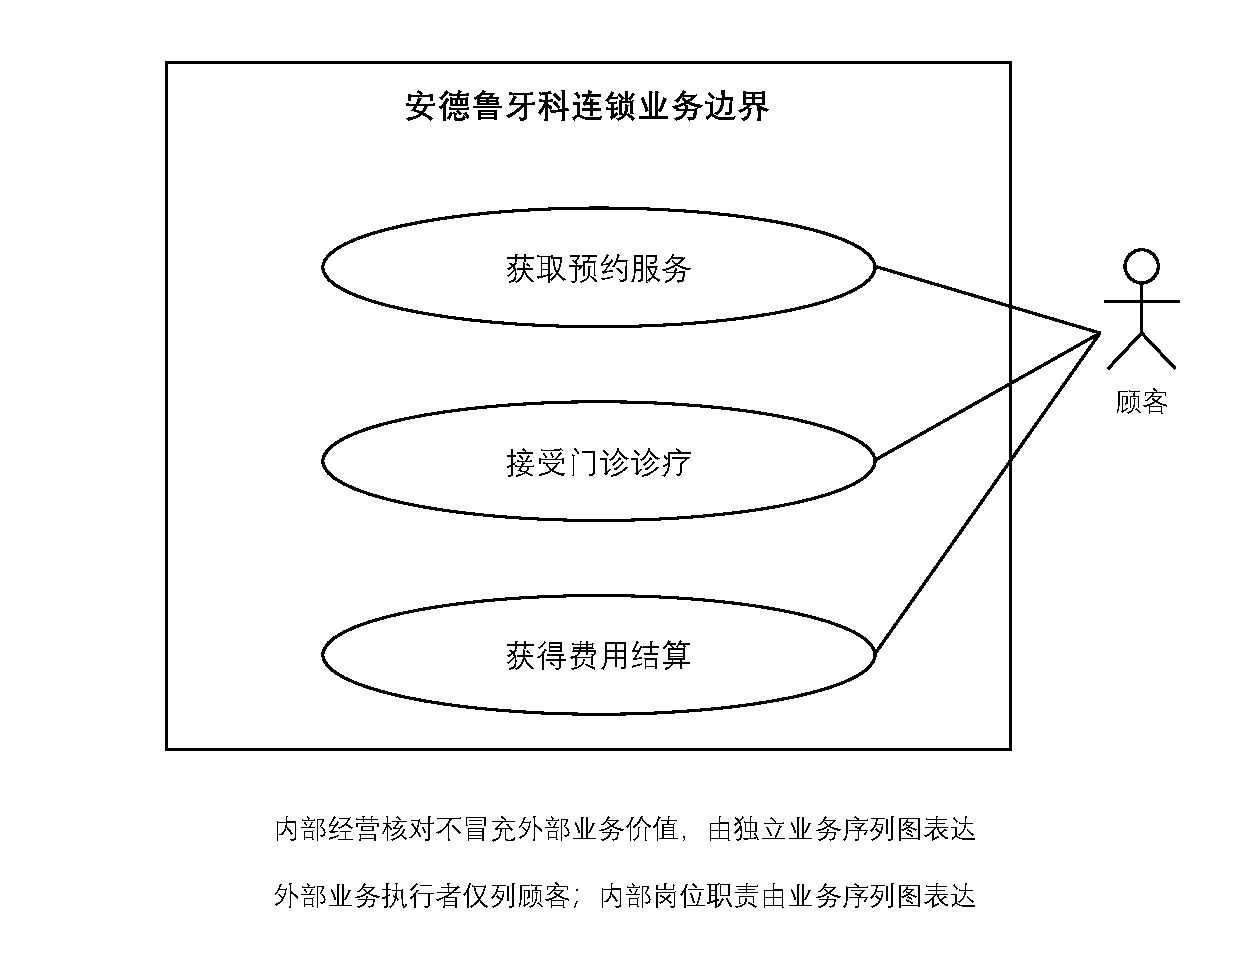
\includegraphics[width=\textwidth]{figures/business_usecases.pdf}
\caption{连锁门诊业务用例图}\label{business_usecases}\end{figure}
\subsection{现状业务流程}
以下现状序列依据案例描述重建，保留人工核对、治疗记录和经营汇总等责任。案例没有说明的具体载体、人员编制和退款制度不作为事实补造；图中的内部岗位名称采用当前项目已确认的四角色映射。序列按预约、就诊与季度管理的不同发生频率拆开。业务消息采用项目约定的虚线箭头，箭头接收者承担该请求的处理责任。\par
\begin{figure}[H]\centering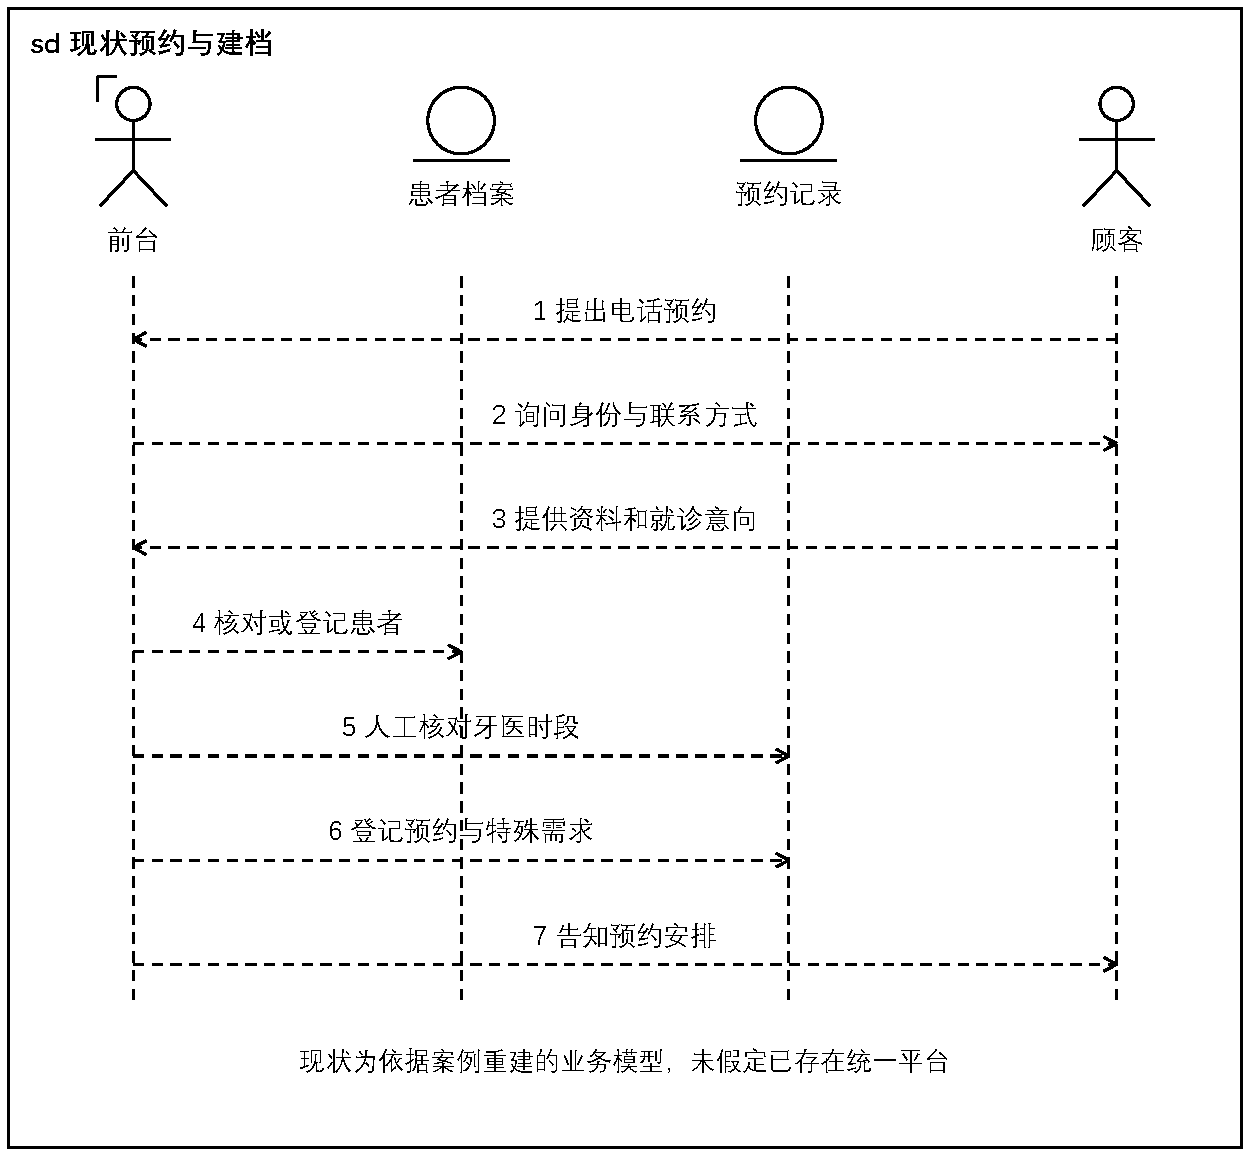
\includegraphics[width=\textwidth]{figures/current_booking.pdf}
\caption{现状预约与建档}\label{current_booking}\end{figure}
\begin{figure}[H]\centering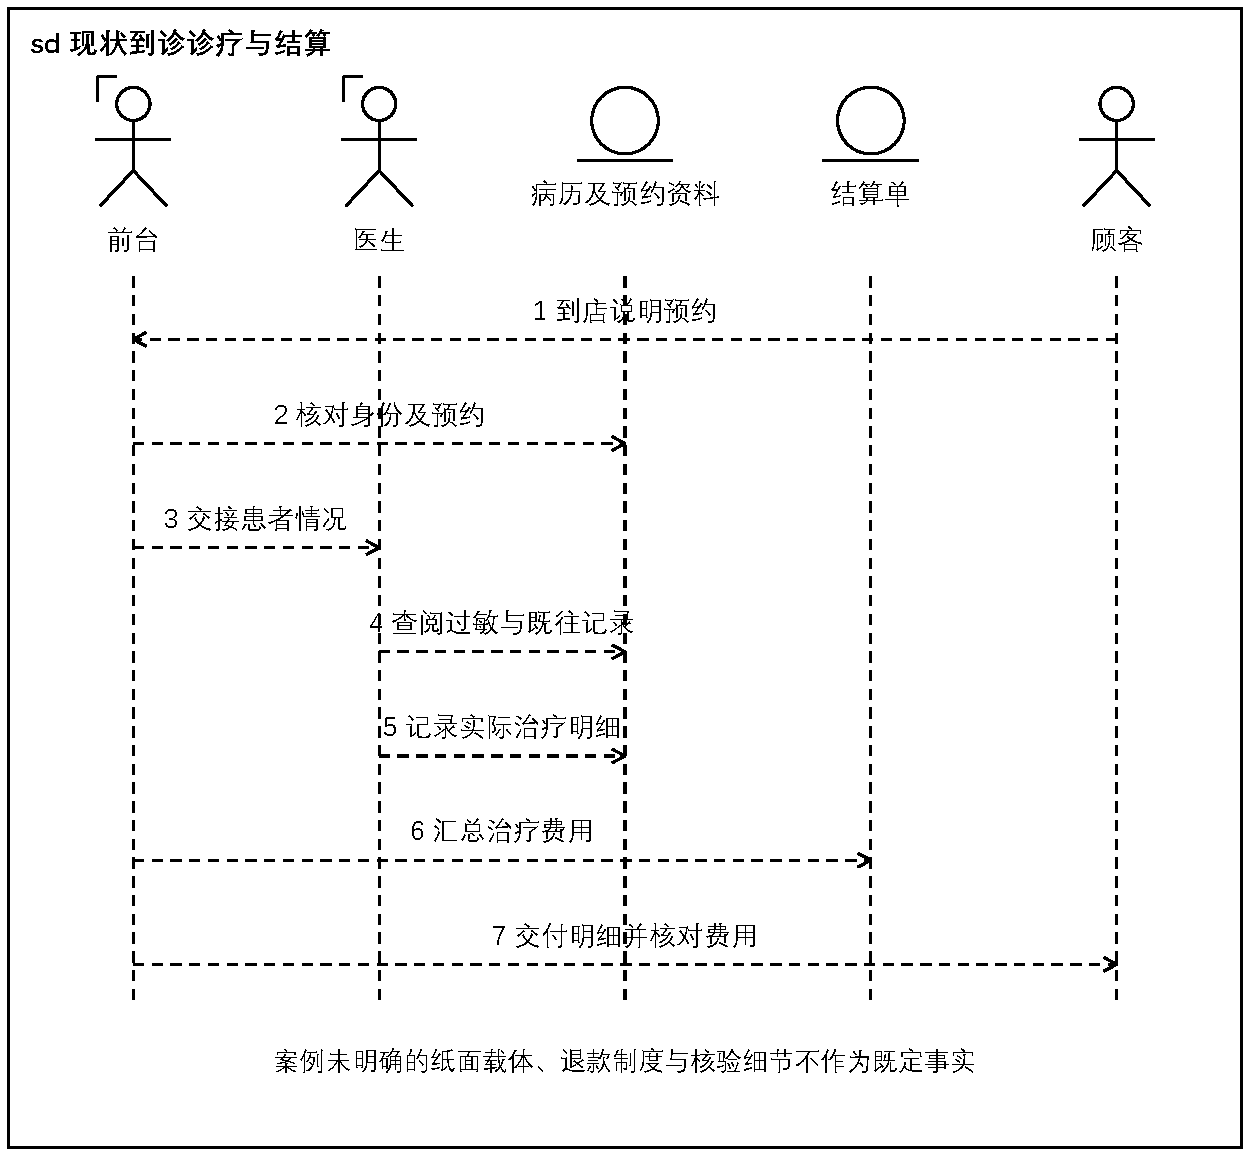
\includegraphics[width=\textwidth]{figures/current_clinical.pdf}
\caption{现状到诊诊疗与结算}\label{current_clinical}\end{figure}
\begin{figure}[H]\centering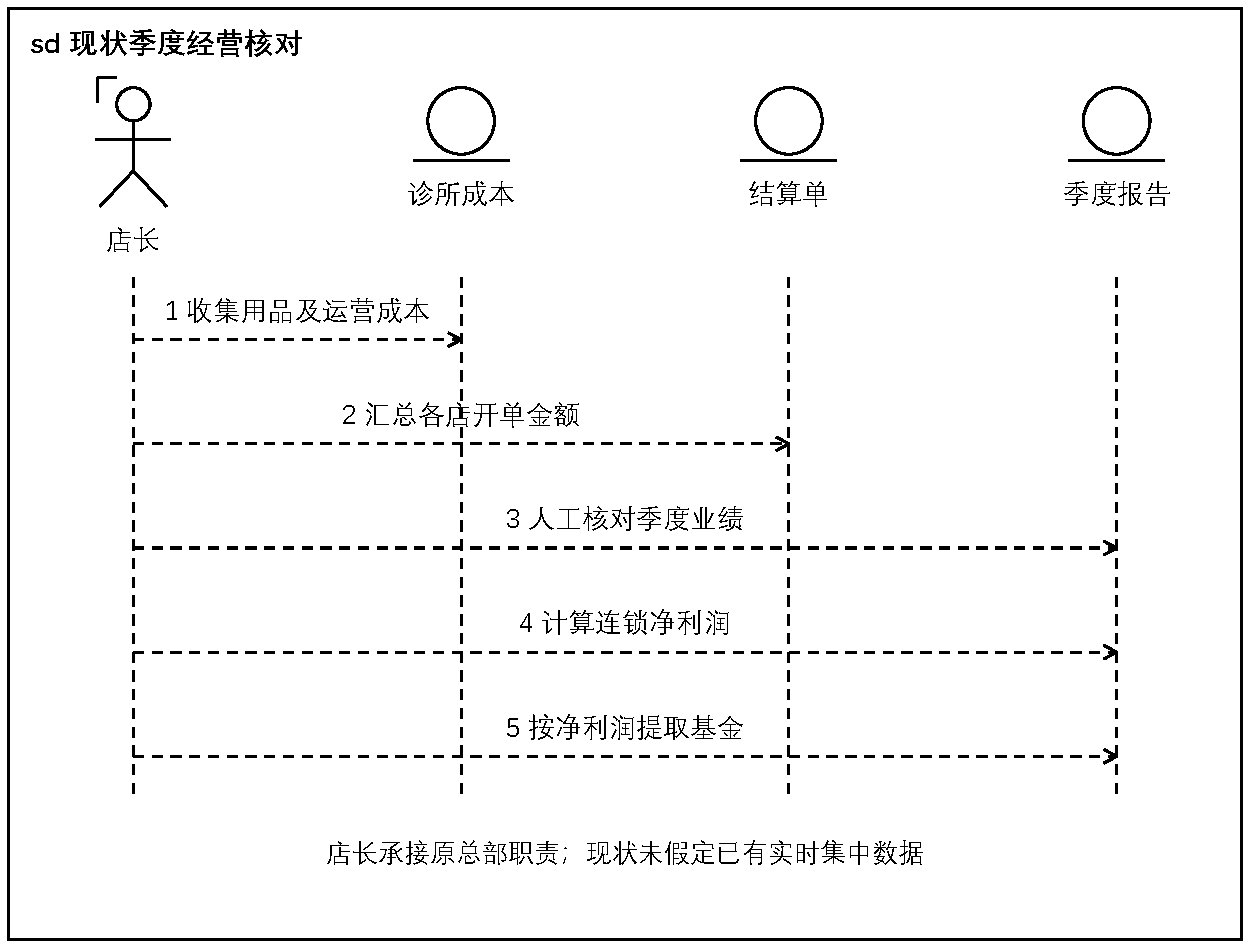
\includegraphics[width=\textwidth]{figures/current_management.pdf}
\caption{现状季度经营核对}\label{current_management}\end{figure}
\subsection{改进业务流程}
改进方案使统一患者编号、号源台账、诊疗明细和财务账簿在各岗位之间复用。身份核验、过敏情况核实和收退款凭据确认仍由有权限的人员负责。目标系统承担信息保存、冲突校验和可追溯记录，不替代医生判断，也不把患者自述自动标为机构核验。\par
\begin{figure}[H]\centering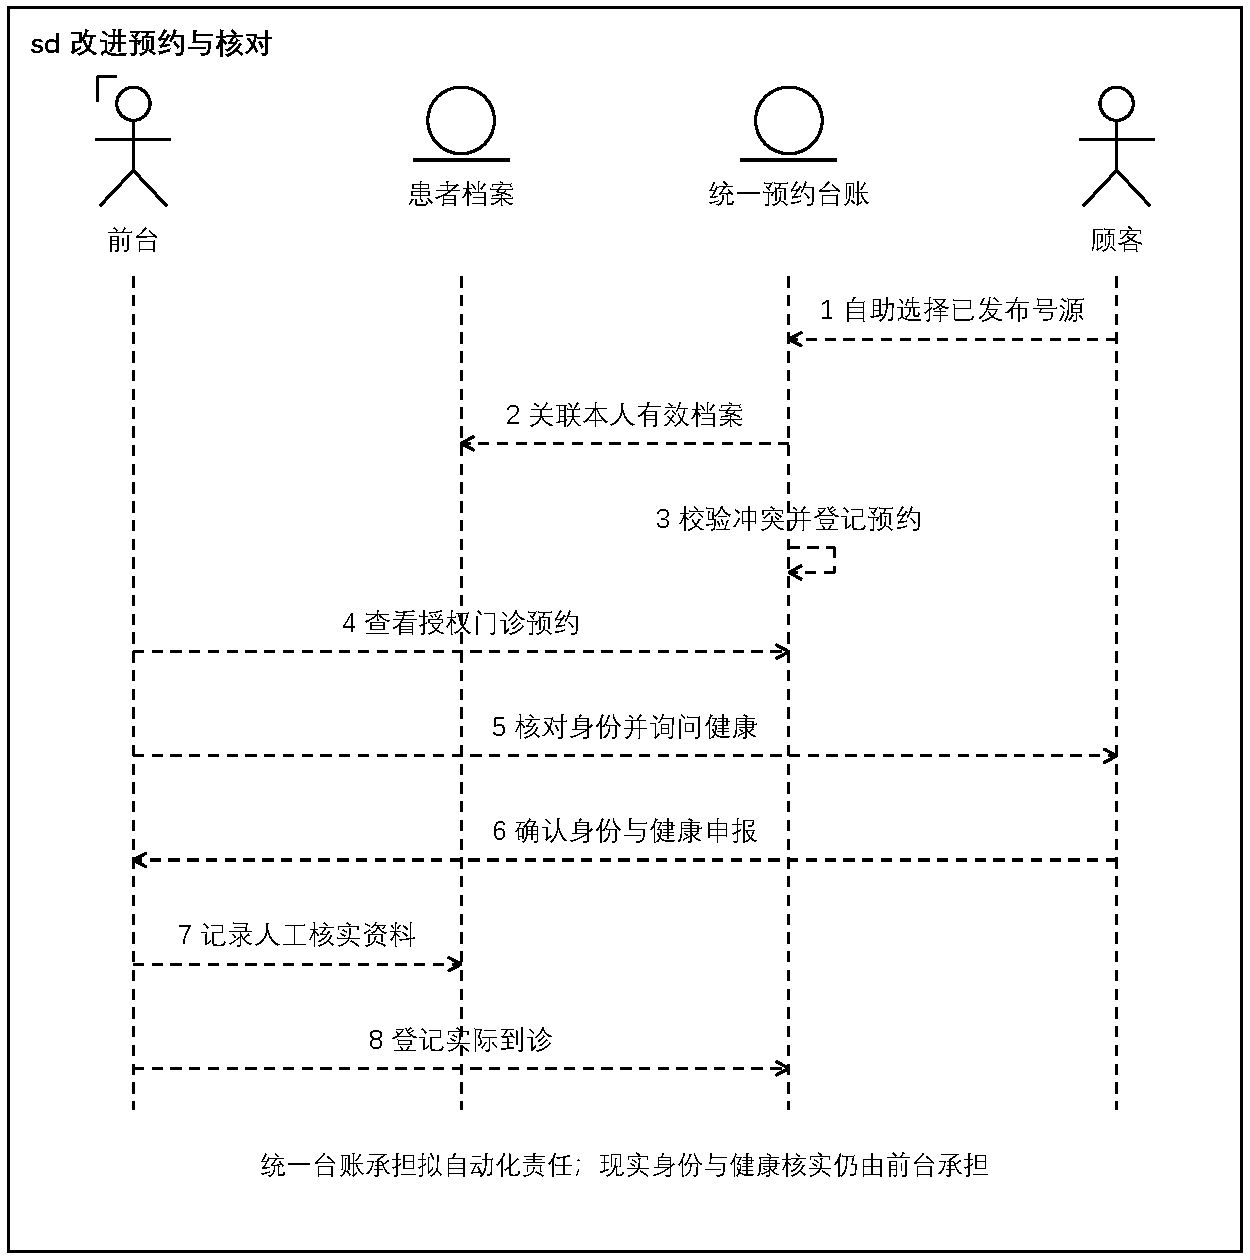
\includegraphics[width=\textwidth]{figures/improved_booking.pdf}
\caption{改进预约与核对}\label{improved_booking}\end{figure}
\begin{figure}[H]\centering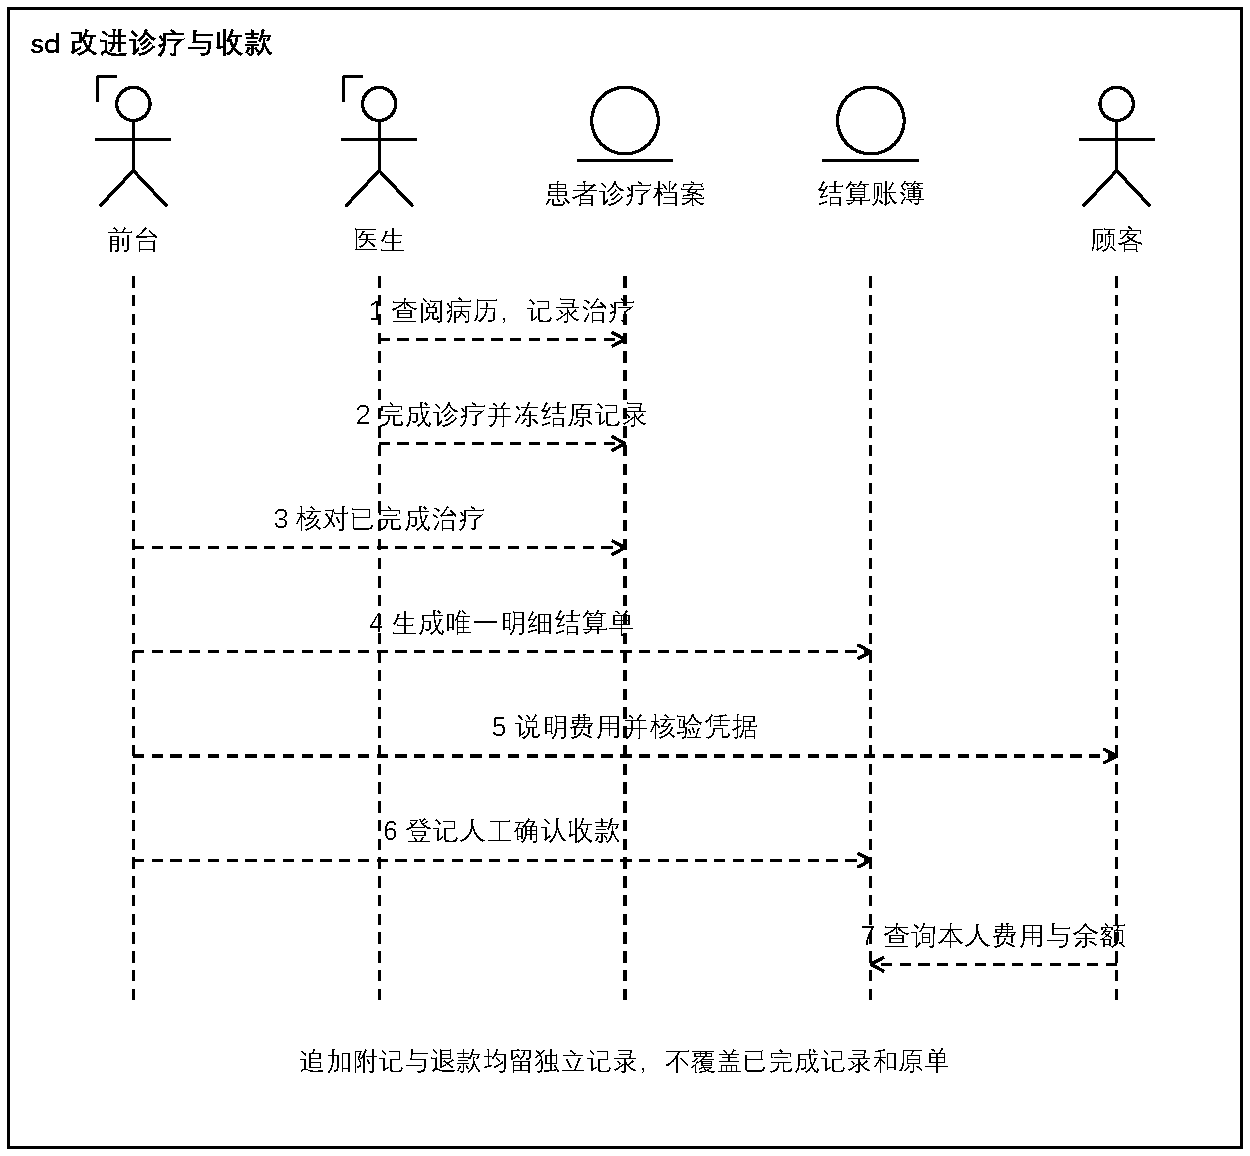
\includegraphics[width=\textwidth]{figures/improved_clinical.pdf}
\caption{改进诊疗与收款}\label{improved_clinical}\end{figure}
\begin{figure}[H]\centering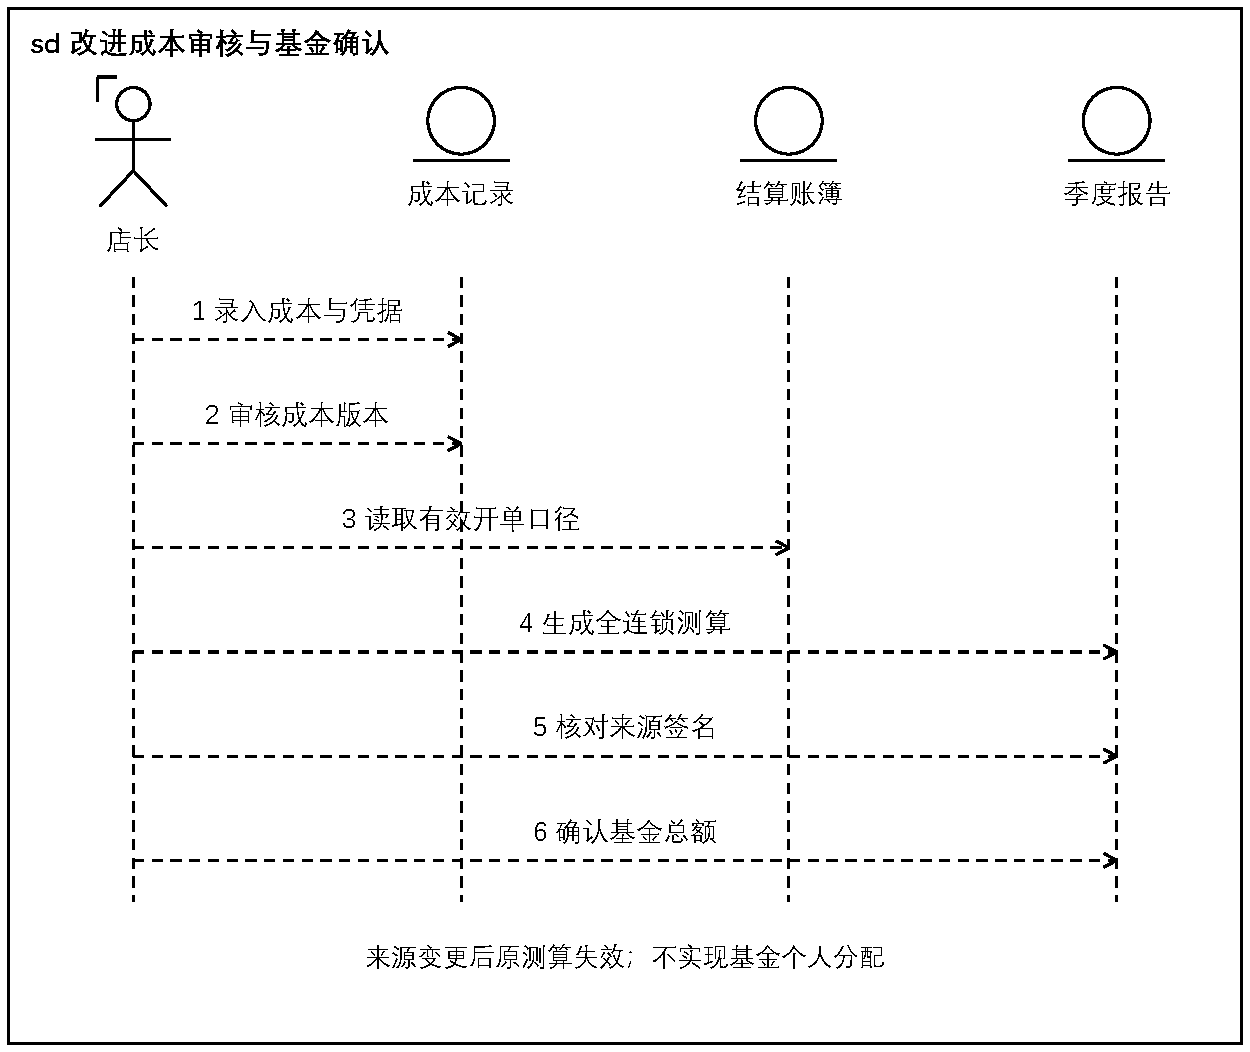
\includegraphics[width=\textwidth]{figures/improved_management.pdf}
\caption{改进成本审核与基金确认}\label{improved_management}\end{figure}
{\fontsize{10.5pt}{15pt}\selectfont\setlength{\tabcolsep}{0pt}\renewcommand{\arraystretch}{1.08}
\begin{longtable}{@{}p{2.840cm}@{\hspace{0.16cm}}p{3.240cm}@{\hspace{0.16cm}}p{5.440cm}@{\hspace{0.16cm}}p{3.440cm}@{}}
\caption{现状与改进的责任对照}\\
\toprule
\bfseries \Cell{现状问题} & \bfseries \Cell{改进责任} & \bfseries \Cell{系统能力} & \bfseries \Cell{仍需人工核实}\\\midrule
\endfirsthead
\toprule
\bfseries \Cell{现状问题} & \bfseries \Cell{改进责任} & \bfseries \Cell{系统能力} & \bfseries \Cell{仍需人工核实}\\\midrule
\endhead
\bottomrule\endlastfoot
\Cell{重复查找患者资料} & \Cell{共享主档案与历史} & \Cell{统一患者编号、过敏明细、跨店授权查询} & \Cell{身份同一性、健康申报}\\[3pt]
\Cell{电话协调易占用冲突时段} & \Cell{提交时统一校验} & \Cell{医生、患者和号源冲突检查及事务} & \Cell{特殊安排与到诊事实}\\[3pt]
\Cell{治疗、开单和收款混淆} & \Cell{按记录阶段分工} & \Cell{完成冻结、费用快照、收款退款分账} & \Cell{治疗确认及资金凭据}\\[3pt]
\Cell{季度汇总口径不一} & \Cell{集中核对来源版本} & \Cell{成本审核、来源签名、全连锁基金} & \Cell{成本归属及管理批准}\\[3pt]
\end{longtable}
}
\Needspace{9\baselineskip}
\section{系统需求与权限}
\subsection{双端边界与四个登录入口}
顾客端提供本人资料、预约、改期取消及本人诊疗费用查询。员工端按前台、医生和店长提供不同工作区。两端共享同一后端与数据库，不是四个分别部署的系统；四个登录地址表达岗位身份，服务端拒绝账号角色与入口不匹配的登录。只有顾客可以公开注册，已有患者电话档案不能被公开认领。\par
{\fontsize{10.5pt}{15pt}\selectfont\setlength{\tabcolsep}{0pt}\renewcommand{\arraystretch}{1.08}
\begin{longtable}{@{}p{1.640cm}@{\hspace{0.16cm}}p{4.140cm}@{\hspace{0.16cm}}p{4.640cm}@{\hspace{0.16cm}}p{4.540cm}@{}}
\caption{角色与门户}\\
\toprule
\bfseries \Cell{角色} & \bfseries \Cell{入口} & \bfseries \Cell{数据范围} & \bfseries \Cell{主要限制}\\\midrule
\endfirsthead
\toprule
\bfseries \Cell{角色} & \bfseries \Cell{入口} & \bfseries \Cell{数据范围} & \bfseries \Cell{主要限制}\\\midrule
\endhead
\bottomrule\endlastfoot
\Cell{顾客} & \Cell{/\allowbreak{}customer/\allowbreak{}login} & \Cell{本人绑定患者} & \Cell{不得访问他人资料或员工功能}\\[3pt]
\Cell{前台} & \Cell{/\allowbreak{}frontdesk/\allowbreak{}login} & \Cell{授权门诊及其合法患者} & \Cell{不能退款、归并、核验绑定或审核成本}\\[3pt]
\Cell{医生} & \Cell{/\allowbreak{}doctor/\allowbreak{}login} & \Cell{本人预约和接诊，授权患者跨店历史} & \Cell{可读历史不等于可改他人诊疗}\\[3pt]
\Cell{店长} & \Cell{/\allowbreak{}manager/\allowbreak{}login} & \Cell{全部门诊} & \Cell{保留版本、状态、核验及有效店长保护}\\[3pt]
\end{longtable}
}
\begin{figure}[H]\centering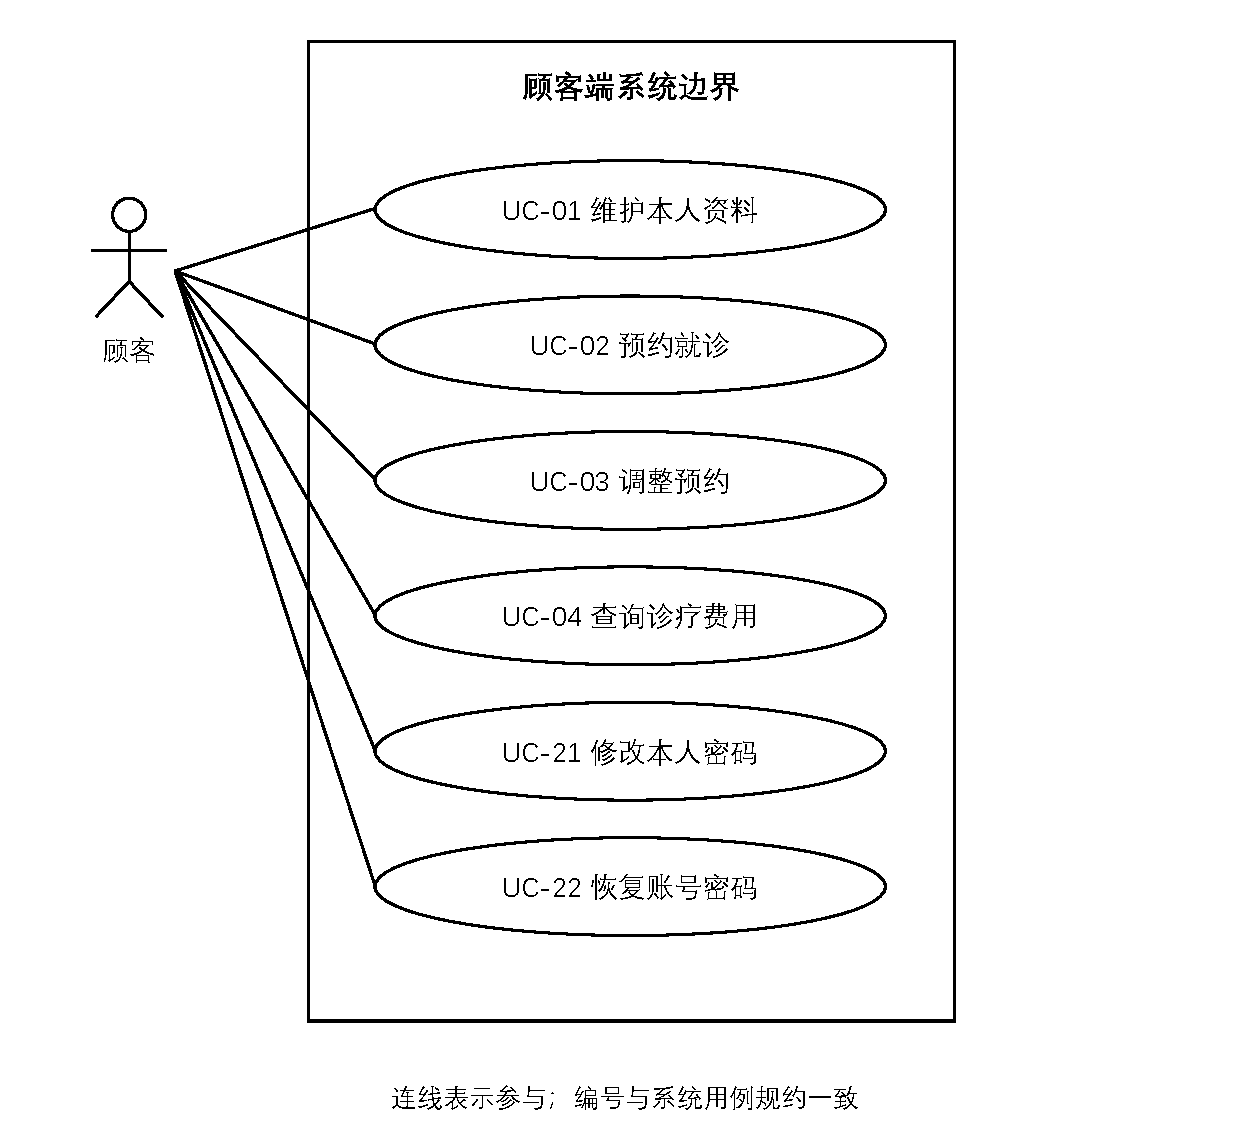
\includegraphics[width=\textwidth]{figures/customer_usecases.pdf}
\caption{顾客端系统边界}\label{customer_usecases}\end{figure}
\begin{figure}[H]\centering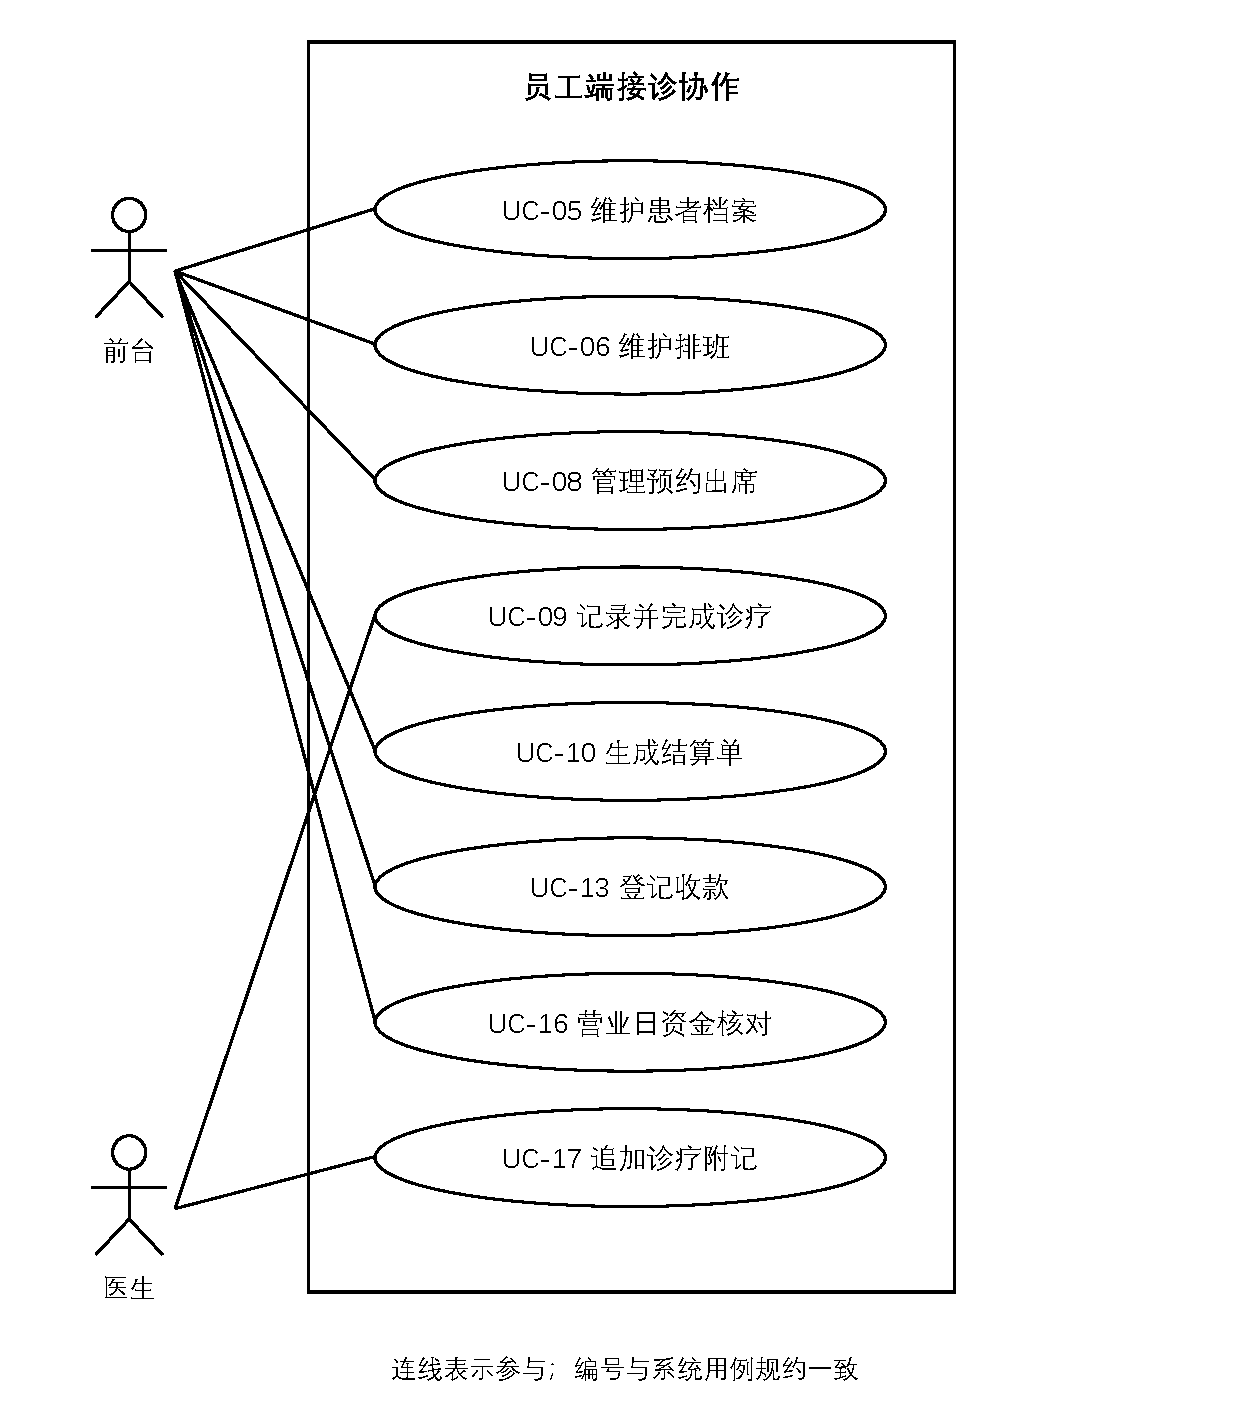
\includegraphics[width=\textwidth]{figures/front_doctor_usecases.pdf}
\caption{员工端接诊协作}\label{front_doctor_usecases}\end{figure}
\begin{figure}[H]\centering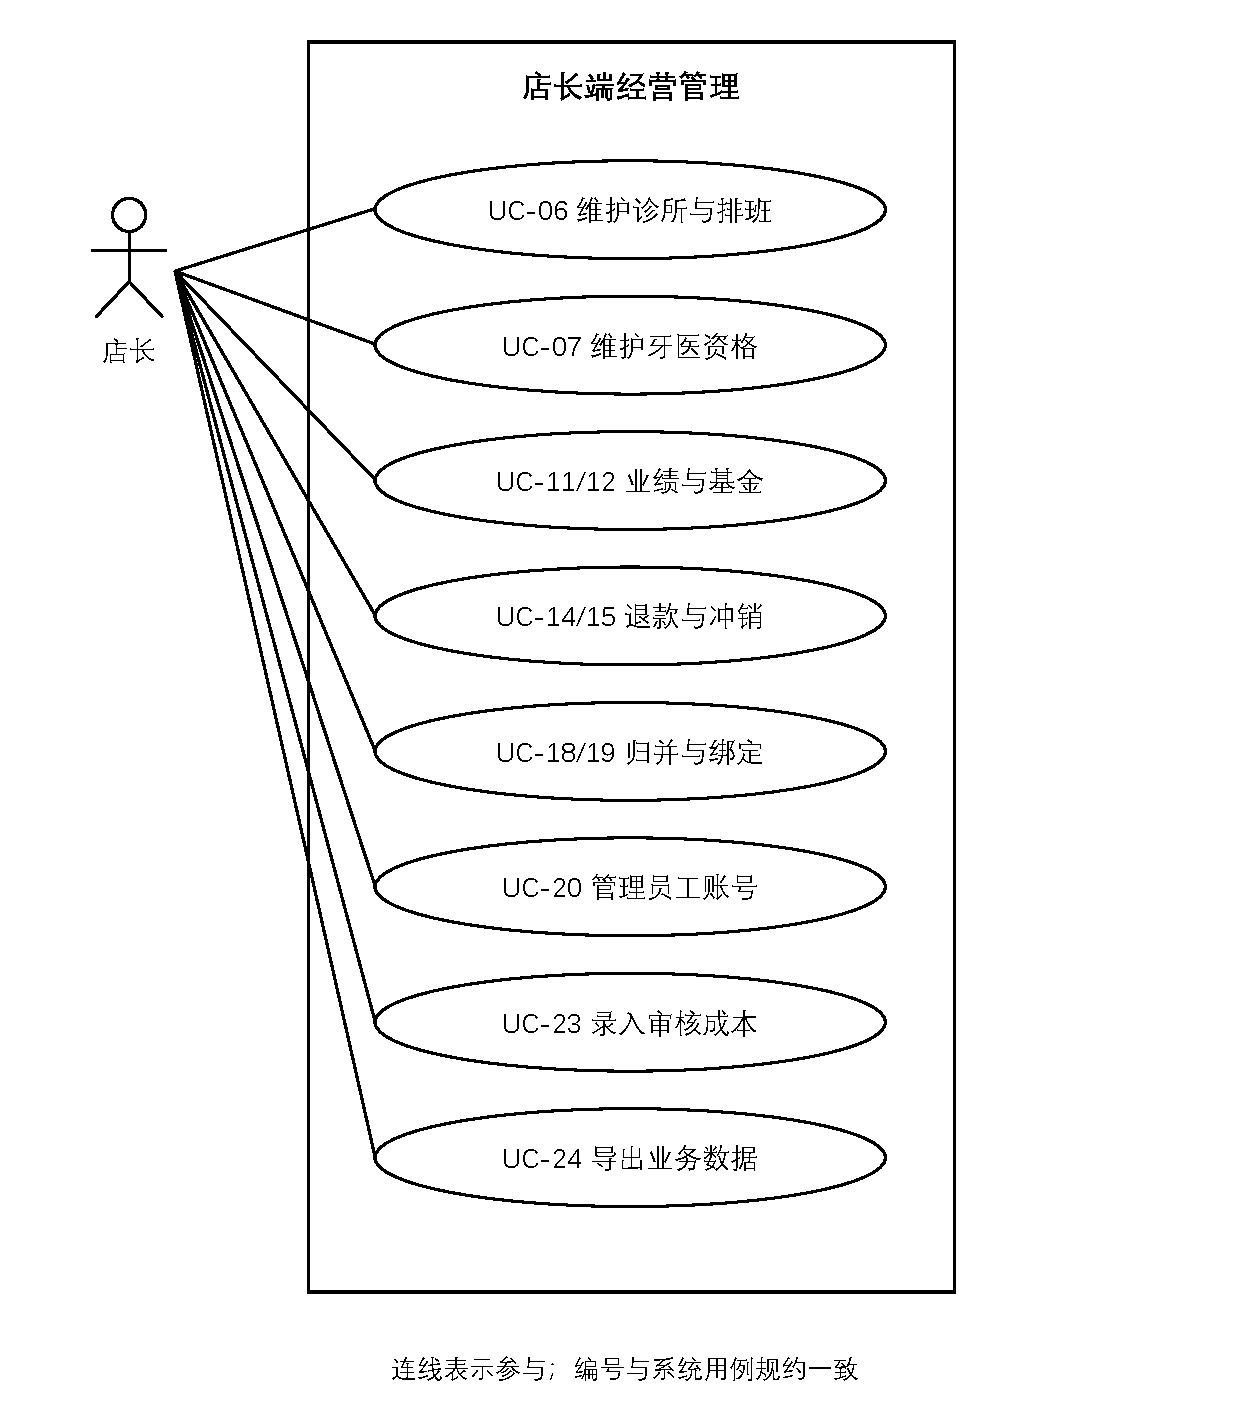
\includegraphics[width=\textwidth]{figures/manager_usecases.pdf}
\caption{店长端经营管理}\label{manager_usecases}\end{figure}
图中为避免拥挤，将员工共同参与的本人改密和恢复用例集中列于用例目录；店长也可执行接待及诊疗相关的授权命令，具体以权限矩阵为准。用例图不表示执行先后，不为增加图形复杂度而虚构include或extend关系。\par
\Needspace{7\baselineskip}
\subsection{系统用例目录}
{\fontsize{10.5pt}{15pt}\selectfont\setlength{\tabcolsep}{0pt}\renewcommand{\arraystretch}{1.08}
\begin{longtable}{@{}p{1.340cm}@{\hspace{0.16cm}}p{3.640cm}@{\hspace{0.16cm}}p{4.040cm}@{\hspace{0.16cm}}p{5.940cm}@{}}
\caption{完整系统用例目录}\\
\toprule
\bfseries \Cell{编号} & \bfseries \Cell{用例名称} & \bfseries \Cell{主执行者} & \bfseries \Cell{涉及业务对象}\\\midrule
\endfirsthead
\toprule
\bfseries \Cell{编号} & \bfseries \Cell{用例名称} & \bfseries \Cell{主执行者} & \bfseries \Cell{涉及业务对象}\\\midrule
\endhead
\bottomrule\endlastfoot
\Cell{UC-01} & \Cell{维护本人就诊资料} & \Cell{顾客（customer）} & \Cell{patients、patient\_\allowbreak{}allergies}\\[3pt]
\Cell{UC-02} & \Cell{预约就诊} & \Cell{顾客（customer）；前台、店长可代办} & \Cell{patients、schedules、appointments、dentist\_\allowbreak{}qualifications、qualifications}\\[3pt]
\Cell{UC-03} & \Cell{调整预约（改期／取消）} & \Cell{顾客（customer）；前台、店长可代办} & \Cell{appointments、schedules、settings、audit}\\[3pt]
\Cell{UC-04} & \Cell{查看本人诊疗与费用} & \Cell{顾客（customer）} & \Cell{visits、visit\_\allowbreak{}lines、visit\_\allowbreak{}addenda、settlements、settlement\_\allowbreak{}lines、payments、refunds、invoice\_\allowbreak{}adjustments}\\[3pt]
\Cell{UC-05} & \Cell{维护患者档案} & \Cell{前台（front）；店长可办理全部门诊} & \Cell{patients、patient\_\allowbreak{}allergies、patient\_\allowbreak{}clinic\_\allowbreak{}access、appointments}\\[3pt]
\Cell{UC-06} & \Cell{维护诊所与排班} & \Cell{店长（manager）；前台仅维护授权门诊排班} & \Cell{clinics、schedules、dentists、qualifications、appointments、quarterReports}\\[3pt]
\Cell{UC-07} & \Cell{维护牙医与资格} & \Cell{店长（manager）} & \Cell{dentists、qualifications、dentist\_\allowbreak{}qualifications、dentist\_\allowbreak{}qualification\_\allowbreak{}details}\\[3pt]
\Cell{UC-08} & \Cell{管理预约与出席} & \Cell{前台（front）；店长可管理全部门诊} & \Cell{appointments、visits、schedules}\\[3pt]
\Cell{UC-09} & \Cell{记录并完成诊疗} & \Cell{医生（clinical）；店长可维护全部就诊} & \Cell{visits、visit\_\allowbreak{}lines、treatments、patients、patient\_\allowbreak{}allergies}\\[3pt]
\Cell{UC-10} & \Cell{生成结算单} & \Cell{前台（front）；店长可办理全部门诊} & \Cell{settlements、settlement\_\allowbreak{}lines、visits、visit\_\allowbreak{}lines、quarterReports}\\[3pt]
\Cell{UC-11} & \Cell{核对季度业绩} & \Cell{店长（manager）} & \Cell{appointments、costs、quarterReports、quarter\_\allowbreak{}report\_\allowbreak{}rows}\\[3pt]
\Cell{UC-12} & \Cell{核算激励基金} & \Cell{店长（manager）} & \Cell{costs、settlements、invoice\_\allowbreak{}adjustments、schedules、quarterReports、quarter\_\allowbreak{}report\_\allowbreak{}rows、quarter\_\allowbreak{}report\_\allowbreak{}settlements、quarter\_\allowbreak{}report\_\allowbreak{}history}\\[3pt]
\Cell{UC-13} & \Cell{登记收款} & \Cell{前台（front）；店长可办理全部门诊} & \Cell{settlements、payments、refunds、invoice\_\allowbreak{}adjustments、idempotency\_\allowbreak{}requests}\\[3pt]
\Cell{UC-14} & \Cell{登记退款} & \Cell{店长（manager）} & \Cell{payments、refunds、settlements、idempotency\_\allowbreak{}requests}\\[3pt]
\Cell{UC-15} & \Cell{冲销结算单} & \Cell{店长（manager）} & \Cell{settlements、invoice\_\allowbreak{}adjustments、payments、refunds、quarterReports}\\[3pt]
\Cell{UC-16} & \Cell{营业日资金核对} & \Cell{前台（front）；店长可核对全部门诊} & \Cell{reconciliations、payments、refunds、settlements}\\[3pt]
\Cell{UC-17} & \Cell{追加诊疗附记} & \Cell{医生（clinical）；店长可为全部已完成就诊追加} & \Cell{visits、visit\_\allowbreak{}addenda、users}\\[3pt]
\Cell{UC-18} & \Cell{归并重复患者} & \Cell{店长（manager）} & \Cell{patients、patient\_\allowbreak{}allergies、patient\_\allowbreak{}clinic\_\allowbreak{}access、appointments、visits、settlements、patient\_\allowbreak{}aliases、users、sessions}\\[3pt]
\Cell{UC-19} & \Cell{核验绑定顾客账号} & \Cell{店长（manager）} & \Cell{patients、users、audit}\\[3pt]
\Cell{UC-20} & \Cell{管理员工账号} & \Cell{店长（manager）} & \Cell{users、clinics、dentists、sessions、password\_\allowbreak{}reset\_\allowbreak{}tokens}\\[3pt]
\Cell{UC-21} & \Cell{修改本人密码} & \Cell{顾客、前台、医生、店长} & \Cell{users、sessions、password\_\allowbreak{}reset\_\allowbreak{}tokens}\\[3pt]
\Cell{UC-22} & \Cell{恢复账号密码} & \Cell{申请人（四种角色）；店长负责核验签发} & \Cell{account\_\allowbreak{}recovery\_\allowbreak{}requests、password\_\allowbreak{}reset\_\allowbreak{}tokens、users、sessions、audit}\\[3pt]
\Cell{UC-23} & \Cell{录入与审核成本} & \Cell{店长（manager）} & \Cell{costs、cost\_\allowbreak{}review\_\allowbreak{}history、quarterReports、quarter\_\allowbreak{}report\_\allowbreak{}history}\\[3pt]
\Cell{UC-24} & \Cell{导出业务数据} & \Cell{店长（manager）} & \Cell{clinics、dentists、qualifications、dentist\_\allowbreak{}qualifications、dentist\_\allowbreak{}qualification\_\allowbreak{}details、treatments、patients、patient\_\allowbreak{}allergies、patient\_\allowbreak{}clinic\_\allowbreak{}access、schedules、appointments、visits、visit\_\allowbreak{}lines、settlements、settlement\_\allowbreak{}lines、costs、cost\_\allowbreak{}review\_\allowbreak{}history、quarterReports、quarter\_\allowbreak{}report\_\allowbreak{}clinics、quarter\_\allowbreak{}report\_\allowbreak{}rows、quarter\_\allowbreak{}report\_\allowbreak{}settlements、quarter\_\allowbreak{}report\_\allowbreak{}history、settings、payments、refunds、invoice\_\allowbreak{}adjustments、reconciliations、visit\_\allowbreak{}addenda、patient\_\allowbreak{}aliases、audit}\\[3pt]
\end{longtable}
}
\Needspace{7\baselineskip}
\subsection{功能权限矩阵}
{\fontsize{10.5pt}{15pt}\selectfont\setlength{\tabcolsep}{0pt}\renewcommand{\arraystretch}{1.08}
\begin{longtable}{@{}p{4.540cm}@{\hspace{0.16cm}}p{2.340cm}@{\hspace{0.16cm}}p{2.640cm}@{\hspace{0.16cm}}p{2.640cm}@{\hspace{0.16cm}}p{2.640cm}@{}}
\caption{服务端岗位权限概览}\\
\toprule
\bfseries \Cell{功能} & \bfseries \Cell{顾客} & \bfseries \Cell{前台} & \bfseries \Cell{医生} & \bfseries \Cell{店长}\\\midrule
\endfirsthead
\toprule
\bfseries \Cell{功能} & \bfseries \Cell{顾客} & \bfseries \Cell{前台} & \bfseries \Cell{医生} & \bfseries \Cell{店长}\\\midrule
\endhead
\bottomrule\endlastfoot
\Cell{本人资料与预约} & \Cell{本人} & \Cell{授权代办} & \Cell{读取本人预约} & \Cell{全门诊}\\[3pt]
\Cell{患者建档和核实} & \Cell{仅本人资料} & \Cell{授权门诊} & \Cell{读取授权患者} & \Cell{全门诊}\\[3pt]
\Cell{资源与排班} & \Cell{读取可预约项} & \Cell{排班} & \Cell{读取本人资源} & \Cell{全部维护}\\[3pt]
\Cell{完成诊疗} & \Cell{—} & \Cell{—} & \Cell{本人接诊} & \Cell{全部授权}\\[3pt]
\Cell{开单与收款} & \Cell{查本人} & \Cell{授权门诊} & \Cell{查相关记录} & \Cell{全部授权}\\[3pt]
\Cell{退款与冲销} & \Cell{—} & \Cell{—} & \Cell{—} & \Cell{是}\\[3pt]
\Cell{营业日资金核对} & \Cell{—} & \Cell{授权门诊} & \Cell{—} & \Cell{全门诊}\\[3pt]
\Cell{完成记录附记} & \Cell{查本人} & \Cell{读授权记录} & \Cell{本人接诊} & \Cell{是}\\[3pt]
\Cell{患者归并与核验绑定} & \Cell{—} & \Cell{—} & \Cell{—} & \Cell{是}\\[3pt]
\Cell{员工生命周期管理} & \Cell{—} & \Cell{—} & \Cell{—} & \Cell{是}\\[3pt]
\Cell{成本审核、季度基金} & \Cell{—} & \Cell{—} & \Cell{—} & \Cell{是}\\[3pt]
\Cell{本人改密、核验恢复} & \Cell{是} & \Cell{是} & \Cell{是} & \Cell{是}\\[3pt]
\end{longtable}
}
矩阵中的“是”仍受对象状态和业务守卫限制。店长不能绕过原款退款上限、机构核验、版本冲突或最后有效店长保护。数据范围在查询服务和业务服务中检查，隐藏页面或按钮仅用于交互引导，不构成授权机制。\par
\Needspace{7\baselineskip}
\subsection{质量需求与设计约束}
{\fontsize{10.5pt}{15pt}\selectfont\setlength{\tabcolsep}{0pt}\renewcommand{\arraystretch}{1.08}
\begin{longtable}{@{}p{1.440cm}@{\hspace{0.16cm}}p{8.140cm}@{\hspace{0.16cm}}p{5.540cm}@{}}
\caption{质量要求与验收范围}\\
\toprule
\bfseries \Cell{编号} & \bfseries \Cell{要求与验收方式} & \bfseries \Cell{当前证据边界}\\\midrule
\endfirsthead
\toprule
\bfseries \Cell{编号} & \bfseries \Cell{要求与验收方式} & \bfseries \Cell{当前证据边界}\\\midrule
\endhead
\bottomrule\endlastfoot
\Cell{QR-01} & \Cell{正确性：关键变更在同一事务内完成，失败无部分业务记录；以冲突、回滚和重放测试验收} & \Cell{有本地自动测试；不代表穷举全部真实场景}\\[3pt]
\Cell{QR-02} & \Cell{安全性：跨角色和跨对象访问由服务端拒绝；敏感凭证不进入审计和业务导出} & \Cell{本地权限、恢复、CSRF和幂等验证}\\[3pt]
\Cell{QR-03} & \Cell{可用性：四入口清楚、错误可理解；390px宽关键路径无横向溢出} & \Cell{有浏览器回归，仍需实际岗位试用}\\[3pt]
\Cell{QR-04} & \Cell{性能：列表分页默认25、上限100；以真实规模下p95和资源消耗另设上线门槛} & \Cell{仅100次、并发10的合成只读测量}\\[3pt]
\Cell{QR-05} & \Cell{可恢复性：一致快照、旧库保留、恢复前副本升级和会话撤销} & \Cell{维护回归通过；未做异地灾难演练}\\[3pt]
\Cell{QR-06} & \Cell{可维护性：模块边界、迁移校验和、可复现构建、源码发布清单} & \Cell{已有代码和本地构建；远端CI尚未执行}\\[3pt]
\end{longtable}
}
四角色、店长全门诊及仅顾客公开注册属于已确认的业务范围。选择原生浏览器模块、Node.\allowbreak{}js、SQLite单实例和CSS构建是本项目的实现方案，不冒充医院或课件强制指定的技术约束。没有现场需求依据的响应时间、可用率和恢复时限不填写为承诺。\par
\section{系统用例规约}
规约按照课件物理页154的完整模板编写，保留前后置条件、涉众利益、基本路径、步骤扩展、字段、业务规则、质量需求及约束。基本路径描述执行者输入与系统责任；具体按钮、弹窗和页面布局在表示层设计中说明。各条规则来自当前实现，局部测试引用表示已有覆盖依据。\par
\Needspace{7\baselineskip}
\subsection{UC-01 维护本人就诊资料}
{\fontsize{10.5pt}{15pt}\selectfont\setlength{\tabcolsep}{0pt}\renewcommand{\arraystretch}{1.08}
\begin{longtable}{@{}p{2.540cm}@{\hspace{0.16cm}}p{12.740cm}@{}}
\toprule
\bfseries \Cell{项目} & \bfseries \Cell{规约内容}\\\midrule
\endfirsthead
\toprule
\bfseries \Cell{项目} & \bfseries \Cell{规约内容}\\\midrule
\endhead
\bottomrule\endlastfoot
\Cell{目标及执行者} & \Cell{顾客在预约前补全本人身份、联系及过敏声明，使接诊人员获得可核对的资料。 主执行者：顾客（customer）}\\[3pt]
\Cell{触发与前置} & \Cell{顾客选择“本人资料”，或预约因资料不完整转入补全。 已通过顾客入口登录并绑定有效患者档案。}\\[3pt]
\Cell{涉众利益} & \Cell{顾客希望资料准确且仅由本人维护。；前台和医生需要联系信息、紧急联系人及过敏来源。}\\[3pt]
\Cell{成功保证} & \Cell{本人资料和过敏明细保存，版本递增，页面显示保存结果。}\\[3pt]
\Cell{最小保证} & \Cell{校验不通过时不覆盖原档案，也不将患者自述记作机构核验。}\\[3pt]
\end{longtable}
}
基本路径：\par
1）顾客打开本人资料页，系统显示已有资料及过敏声明状态。\par
2）顾客选择编辑，输入姓名、出生日期、电话、地址和紧急联系人。\par
3）顾客选择过敏状态；已知过敏时逐项输入过敏项、反应及备注。\par
4）顾客核对表单并提交，系统依据当前会话确定患者，不接受他人档案。\par
5）系统检查资料格式、过敏声明与明细的一致性及原版本。\par
6）系统保存档案和过敏明细，记录声明时间及“患者自述”来源。\par
7）系统显示更新后的资料；顾客继续预约或结束维护。\par
扩展3a：顾客不能确定过敏情况。顾客选择“待核实”并提交声明；系统保留未核验状态。 返回主流程第4步。\par
扩展5b：档案已被他人更新或已归并。系统拒绝覆盖并提示刷新；顾客重新读取主档案后核对。 返回主流程第1步，或结束。\par
字段列表：输入 id：本人档案编号，必填；输入 version：必填，当前整数版本；输入 name：必填，≤60字符；输入 dob：可空；非未来 YYYY-MM-DD；输入 phone：必填，有效电话；输入 email：可选，有效邮箱；输入 address：可选，≤300字符；输入 emergencyName/\allowbreak{}emergencyPhone：可选；预约前须补全；输入 allergyStatus：unknown/\allowbreak{}none/\allowbreak{}known；输入 allergies：数组≤30项；name必填，reaction/\allowbreak{}note可选；输出 result.\allowbreak{}id/\allowbreak{}version：档案编号与递增版本；输出 result.\allowbreak{}allergies：保存后的过敏明细；输出 result.\allowbreak{}allergySource：患者自述及未核验状态\par
业务规则：顾客只能修改绑定的本人档案，不能自行新增第二份档案。；过敏状态为 unknown、none、known；known 至少一项，其他状态不得带明细。；患者自述不设置工作人员核验者和核验时间；更新须提交原版本。\par
质量要求：系统应阻止越权与旧版本覆盖，保留声明来源。\par
约束与方案：系统按用户要求仅设顾客、前台、医生、店长，店长覆盖全部门诊。；系统当前以会话绑定患者，过敏声明和明细分表保存。\par
实现与验证依据：server/\allowbreak{}services/\allowbreak{}patients.\allowbreak{}js：patient.\allowbreak{}save；public/\allowbreak{}js/\allowbreak{}pages/\allowbreak{}patients.\allowbreak{}js；GET /\allowbreak{}api/\allowbreak{}workspace?page=profile。test/\allowbreak{}system.\allowbreak{}test.\allowbreak{}js：注册、多项过敏与旧版本保护；未知过敏声明预约。\par
\Needspace{7\baselineskip}
\subsection{UC-02 预约就诊}
{\fontsize{10.5pt}{15pt}\selectfont\setlength{\tabcolsep}{0pt}\renewcommand{\arraystretch}{1.08}
\begin{longtable}{@{}p{2.540cm}@{\hspace{0.16cm}}p{12.740cm}@{}}
\toprule
\bfseries \Cell{项目} & \bfseries \Cell{规约内容}\\\midrule
\endfirsthead
\toprule
\bfseries \Cell{项目} & \bfseries \Cell{规约内容}\\\midrule
\endhead
\bottomrule\endlastfoot
\Cell{目标及执行者} & \Cell{为本人或已授权患者选择可用牙医时段，形成可追踪且无时间冲突的有效预约。 主执行者：顾客（customer）；前台、店长可代办}\\[3pt]
\Cell{触发与前置} & \Cell{参与者进入预约页面并选择预约对象。 已登录；患者为有效主档案；姓名、出生日期、联系地址、紧急联系人和过敏声明满足预约要求。}\\[3pt]
\Cell{涉众利益} & \Cell{患者需要明确的诊所、牙医和就诊时间。；门诊和牙医需要避免时段重叠及重复占位。}\\[3pt]
\Cell{成功保证} & \Cell{建立有效预约并显示编号、诊所、牙医及时间。}\\[3pt]
\Cell{最小保证} & \Cell{任何检查失败均不占用时段；并发提交不会产生两个有效预约。}\\[3pt]
\end{longtable}
}
基本路径：\par
1）参与者打开预约页，系统显示授权患者和未来可预约时段。\par
2）参与者选择患者，并按门诊、牙医或日期筛选，系统显示可用名额。\par
3）参与者选择时段，输入就诊问题及可选的特殊需求。\par
4）系统显示预约摘要，参与者核对后提交预约。\par
5）系统检查患者资料、资源状态、有效资格及患者和牙医时间冲突。\par
6）系统在事务内核对剩余容量并建立 booked 状态预约。\par
7）系统显示预约成功信息，参与者可在预约列表继续查看。\par
扩展5a：资料不完整。系统说明缺项；顾客进入 UC-01，工作人员进入 UC-05 补充核对。 资料补齐后返回第1步。\par
扩展6b：时段已满或出现重叠。系统不建立预约，显示需重新选时段的信息。 返回主流程第2步。\par
字段列表：输入 patientId：本人或授权患者编号；输入 scheduleId：必填，可用未来时段编号；输入 problem：必填，≤1000字符；输入 specialNeeds：可选，≤1000字符；输出 result.\allowbreak{}id/\allowbreak{}status：预约编号；状态 booked；输出 result.\allowbreak{}clinicId/\allowbreak{}dentistId：门诊和牙医编号；输出 result.\allowbreak{}start/\allowbreak{}end：ISO起止时间；界面按北京时间显示；输出 result.\allowbreak{}version：初始版本1\par
业务规则：顾客只能预约本人；前台只能在分配门诊代办。；仅未来、启用门诊、启用牙医且存在有效资格的时段可约。；单牙医时段容量固定为1；患者与牙医的 booked、attended 预约均参与冲突判断。\par
质量要求：系统应以同一事务核对占位与建约，防止并发超订。\par
约束与方案：系统按用户要求仅设顾客、前台、医生、店长，店长覆盖全部门诊。；系统当前采用单牙医单名额时段，并由后端执行范围校验。\par
实现与验证依据：server/\allowbreak{}services/\allowbreak{}appointments.\allowbreak{}js：appointment.\allowbreak{}book；public/\allowbreak{}js/\allowbreak{}pages/\allowbreak{}appointments.\allowbreak{}js；public/\allowbreak{}js/\allowbreak{}pages/\allowbreak{}booking-picker.\allowbreak{}js。test/\allowbreak{}system.\allowbreak{}test.\allowbreak{}js：竞争预约原子性、未知过敏声明及跨门诊档案检索。\par
\Needspace{7\baselineskip}
\subsection{UC-03 调整预约（改期／取消）}
{\fontsize{10.5pt}{15pt}\selectfont\setlength{\tabcolsep}{0pt}\renewcommand{\arraystretch}{1.08}
\begin{longtable}{@{}p{2.540cm}@{\hspace{0.16cm}}p{12.740cm}@{}}
\toprule
\bfseries \Cell{项目} & \bfseries \Cell{规约内容}\\\midrule
\endfirsthead
\toprule
\bfseries \Cell{项目} & \bfseries \Cell{规约内容}\\\midrule
\endhead
\bottomrule\endlastfoot
\Cell{目标及执行者} & \Cell{按业务规则取消有效预约，或将同一就诊需求改到其他可用时段。 主执行者：顾客（customer）；前台、店长可代办}\\[3pt]
\Cell{触发与前置} & \Cell{参与者在预约列表选择一项有效预约的改期或取消操作。 已登录并有权操作该预约；预约状态为 booked。}\\[3pt]
\Cell{涉众利益} & \Cell{患者希望变更时间后能够确认新的安排。；前台需要保留取消原因和改约前后关系。}\\[3pt]
\Cell{成功保证} & \Cell{取消时保留原预约及原因；改期时建立关联的新预约，旧预约标记取消。}\\[3pt]
\Cell{最小保证} & \Cell{改期失败时原预约保持有效，不出现仅取消却未成功改约的中间结果。}\\[3pt]
\end{longtable}
}
基本路径：\par
1）系统显示预约列表，参与者选择待调整预约。\par
2）系统显示原门诊、牙医、时间和取消截止规则。\par
3）参与者选择取消或改期并输入原因；改期时继续选择新的可用时段。\par
4）系统显示变更摘要，参与者核对并提交。\par
5）系统核对对象权限、版本、有效状态及顾客自助截止时间。\par
6）系统以事务保存取消；改期还重新校验新时段并建立 previousId 关联。\par
7）系统显示取消结果或新预约详情，参与者核对安排后结束。\par
扩展5a：顾客已超过自助截止时间。系统拒绝自助变更并提示联系门诊，由授权前台另行处理。 本次自助流程结束。\par
扩展6b：新时段不可用。系统回滚整个改期事务，原预约仍有效。 返回主流程第3步重选。\par
字段列表：输入 id/\allowbreak{}version：必填，原预约及当前整数版本；输入 reason：必填，≤500字符；输入 scheduleId：改期必填；取消不传；输出 result.\allowbreak{}id/\allowbreak{}status：取消返回原记录；改期返回新预约；输出 result.\allowbreak{}previousId：改期返回原预约编号；输出 result.\allowbreak{}cancelReason：取消时返回原因；输出 result.\allowbreak{}version：操作后记录版本\par
业务规则：只有 booked 预约可取消或改期；已到诊和爽约不直接走此流程。；自助截止小时数取 settings.\allowbreak{}cancellationHours，允许店长设置0至168。；改期沿用原就诊问题、特殊需求，并保留旧记录及审计关联。\par
质量要求：系统应在改约失败时回滚取消，保留原占位。\par
约束与方案：系统按用户要求仅设顾客、前台、医生、店长，店长覆盖全部门诊。；系统当前以取消旧约、新建关联预约实现改期，自助期限由统一设置决定。\par
实现与验证依据：server/\allowbreak{}services/\allowbreak{}appointments.\allowbreak{}js：appointment.\allowbreak{}cancel、appointment.\allowbreak{}reschedule；public/\allowbreak{}js/\allowbreak{}pages/\allowbreak{}appointments.\allowbreak{}js。test/\allowbreak{}system.\allowbreak{}test.\allowbreak{}js：竞争预约及失败改期恢复原预约；test/\allowbreak{}calendar.\allowbreak{}test.\allowbreak{}js：取消记录不占位。\par
\Needspace{7\baselineskip}
\subsection{UC-04 查看本人诊疗与费用}
{\fontsize{10.5pt}{15pt}\selectfont\setlength{\tabcolsep}{0pt}\renewcommand{\arraystretch}{1.08}
\begin{longtable}{@{}p{2.540cm}@{\hspace{0.16cm}}p{12.740cm}@{}}
\toprule
\bfseries \Cell{项目} & \bfseries \Cell{规约内容}\\\midrule
\endfirsthead
\toprule
\bfseries \Cell{项目} & \bfseries \Cell{规约内容}\\\midrule
\endhead
\bottomrule\endlastfoot
\Cell{目标及执行者} & \Cell{顾客查询本人历史就诊、治疗明细、结算及收退款状态，核对费用并按需打印结算单。 主执行者：顾客（customer）}\\[3pt]
\Cell{触发与前置} & \Cell{顾客选择诊疗历史或费用页面。 已通过顾客入口登录；账号绑定本人患者档案。}\\[3pt]
\Cell{涉众利益} & \Cell{顾客需要理解治疗内容、原开单金额、实际收款和欠款。；门诊需要向顾客提供同一来源的就诊费用信息。}\\[3pt]
\Cell{成功保证} & \Cell{显示本人被授权读取的诊疗、附记和账单信息；可打开打印视图。}\\[3pt]
\Cell{最小保证} & \Cell{不因知道他人编号而暴露他人的诊疗与账务；查询不改写历史。}\\[3pt]
\end{longtable}
}
基本路径：\par
1）顾客进入历史或费用页，系统按本人范围显示分页列表。\par
2）顾客选择页码并提交查询，系统显示关联门诊、牙医和就诊时间。\par
3）顾客打开诊疗详情，系统显示治疗项目、数量、备注及已有附记。\par
4）顾客选择对应结算单，系统显示项目价格快照和开单总额。\par
5）系统同时显示应收、净实收、欠款及冲销状态，顾客逐项核对。\par
6）顾客选择打印时，系统展示结算单打印内容并交由浏览器打印。\par
7）顾客关闭详情或继续查询，系统保留当前页面查询条件。\par
扩展2a：没有符合条件的记录。系统显示空状态；顾客调整查询或结束。 返回第1步或结束。\par
扩展4b：就诊尚未开单。系统保留诊疗内容并提示尚无结算单。 返回第2步，不生成账单。\par
字段列表：输入 page：history或settlements；输入 limit/\allowbreak{}offset：可选；默认25/\allowbreak{}0，limit≤100；输入 clinicId/\allowbreak{}dentistId/\allowbreak{}date：费用查询可选筛选；日期 YYYY-MM-DD；输入 选中记录编号：限本次授权查询所得记录；输出 visits/\allowbreak{}visitAddenda：本人诊疗和附记；输出 settlements/\allowbreak{}financeSummaries：金额整数分，含应收、净实收、欠款；输出 pagination：总数及当前分页范围；输出 打印内容：所选单据展示内容\par
业务规则：服务端按 patientId 限定顾客的预约、诊疗与结算读取。；开单总额与收款分开显示；结算单不代替正式医疗收费票据。；历史治疗价格取已记录快照，不随目录调价追溯改变。\par
质量要求：系统应保护患者隐私并保持治疗、费用来源一致。\par
约束与方案：系统按用户要求仅设顾客、前台、医生、店长，店长覆盖全部门诊。；系统当前按页读取同一后端；打印由浏览器处理，不生成正式收费票据。\par
实现与验证依据：server/\allowbreak{}services/\allowbreak{}workspace.\allowbreak{}js：history、settlements；public/\allowbreak{}js/\allowbreak{}pages/\allowbreak{}clinical.\allowbreak{}js；public/\allowbreak{}js/\allowbreak{}pages/\allowbreak{}billing.\allowbreak{}js。test/\allowbreak{}system.\allowbreak{}test.\allowbreak{}js：本人范围保护、完整诊疗结算链及重启持久化；打印行为未单独覆盖。\par
\Needspace{7\baselineskip}
\subsection{UC-05 维护患者档案}
{\fontsize{10.5pt}{15pt}\selectfont\setlength{\tabcolsep}{0pt}\renewcommand{\arraystretch}{1.08}
\begin{longtable}{@{}p{2.540cm}@{\hspace{0.16cm}}p{12.740cm}@{}}
\toprule
\bfseries \Cell{项目} & \bfseries \Cell{规约内容}\\\midrule
\endfirsthead
\toprule
\bfseries \Cell{项目} & \bfseries \Cell{规约内容}\\\midrule
\endhead
\bottomrule\endlastfoot
\Cell{目标及执行者} & \Cell{工作人员检索、核对和维护授权患者资料，跨门诊就诊优先复用既有档案。 主执行者：前台（front）；店长可办理全部门诊}\\[3pt]
\Cell{触发与前置} & \Cell{前台为患者办理预约、资料更正或跨门诊接诊。 已登录工作人员入口；前台有分配门诊，店长管理全部门诊。}\\[3pt]
\Cell{涉众利益} & \Cell{患者希望跨门诊就诊时不重复建档。；医生需要有来源的过敏声明；店长需要可追踪的资料变更。}\\[3pt]
\Cell{成功保证} & \Cell{新增或更新档案；核对成功时为前台门诊授予既有档案访问范围。}\\[3pt]
\Cell{最小保证} & \Cell{未核对成功不擅自认领跨门诊档案；已有归并档案不再改写。}\\[3pt]
\end{longtable}
}
基本路径：\par
1）工作人员进入患者页，系统显示授权范围内的患者列表。\par
2）工作人员输入姓名、电话或编号检索，系统显示匹配结果。\par
3）跨门诊未找到时，工作人员输入联系电话和出生日期进行精确核对。\par
4）系统显示唯一匹配档案，或工作人员选择新增患者并录入基本信息。\par
5）工作人员核对身份、联系与过敏资料，输入更正内容并提交。\par
6）系统检查权限、版本和声明明细，在事务中保存档案及明细。\par
7）系统显示保存后的患者信息，工作人员继续预约或结束。\par
扩展3a：无匹配或存在多份匹配档案。系统不自动授予访问；无匹配可核实后建档，多份匹配转店长 UC-18。 返回第2步，或结束并转交。\par
扩展6b：版本已变化。系统拒绝覆盖，工作人员刷新并重新核对。 返回主流程第1步。\par
字段列表：输入 id/\allowbreak{}version：新增可不传；更新必填；输入 phone/\allowbreak{}dob：跨门诊检索必填，日期 YYYY-MM-DD；输入 name：保存必填，≤60字符；输入 clinicId：新增可选，限授权门诊；输入 email/\allowbreak{}address：可选，有效邮箱及≤300字符；输入 emergencyName/\allowbreak{}emergencyPhone：可选，预约前须补全；输入 allergyStatus/\allowbreak{}allergies：状态和明细须一致；输出 result.\allowbreak{}id/\allowbreak{}version：新建或更新的档案及版本；输出 result.\allowbreak{}accessClinicIds：跨门诊核对后授权范围；输出 result.\allowbreak{}allergyVerifiedBy/\allowbreak{}At：工作人员核对标记或空值\par
业务规则：跨门诊检索使用标准化电话和出生日期，必须唯一匹配。；前台访问限创建门诊、授权门诊或既有预约关系。；工作人员提交非 unknown 过敏状态时记录核验者、时间与来源；不宣称系统自动验证身份。\par
质量要求：系统应防止未核验跨门诊认领，并保留更正审计。\par
约束与方案：系统按用户要求仅设顾客、前台、医生、店长，店长覆盖全部门诊。；系统当前使用电话与生日唯一匹配授予访问，不采用公开档案认领。\par
实现与验证依据：server/\allowbreak{}services/\allowbreak{}patients.\allowbreak{}js：patient.\allowbreak{}lookup、patient.\allowbreak{}save；server/\allowbreak{}services/\allowbreak{}shared.\allowbreak{}js：scopeFor、ensurePatient。test/\allowbreak{}system.\allowbreak{}test.\allowbreak{}js：核验跨门诊检索、范围保护和旧版本保护。\par
\Needspace{7\baselineskip}
\subsection{UC-06 维护诊所与排班}
{\fontsize{10.5pt}{15pt}\selectfont\setlength{\tabcolsep}{0pt}\renewcommand{\arraystretch}{1.08}
\begin{longtable}{@{}p{2.540cm}@{\hspace{0.16cm}}p{12.740cm}@{}}
\toprule
\bfseries \Cell{项目} & \bfseries \Cell{规约内容}\\\midrule
\endfirsthead
\toprule
\bfseries \Cell{项目} & \bfseries \Cell{规约内容}\\\midrule
\endhead
\bottomrule\endlastfoot
\Cell{目标及执行者} & \Cell{维护门诊基本资料和牙医未来接诊时段，使预约资源与实际接诊安排保持一致。 主执行者：店长（manager）；前台仅维护授权门诊排班}\\[3pt]
\Cell{触发与前置} & \Cell{门诊启用、资料变化，或工作人员安排未来接诊时间。 店长已登录；维护排班的前台已获相应门诊授权；牙医和资格资料已建立。}\\[3pt]
\Cell{涉众利益} & \Cell{患者需要可预约的准确时段。；牙医需要跨门诊时间不重叠；门诊需要保留历史安排。}\\[3pt]
\Cell{成功保证} & \Cell{门诊或排班保存并显示新版本；资源范围变化使相关季度报告待重新核算。}\\[3pt]
\Cell{最小保证} & \Cell{已有预约或跨门诊时间冲突时不破坏原接诊安排。}\\[3pt]
\end{longtable}
}
基本路径：\par
1）参与者打开资源页，系统显示可维护的诊所或接诊排班。\par
2）店长选择新增或编辑诊所，输入名称、地址、主管、电话和面积。\par
3）维护排班时，参与者选择门诊、牙医并输入开始及结束时间。\par
4）系统显示容量和开放状态，参与者核对后提交保存。\par
5）系统检查门诊权限、资源启用状态、有效资格及未来时间范围。\par
6）系统核对牙医跨门诊时段和已有预约约束后保存资源。\par
7）系统显示最新资源列表，参与者确认后结束维护。\par
扩展5a：排班时间与同一牙医其他有效排班重叠。系统说明冲突并拒绝保存。 返回第3步调整时间。\par
扩展6b：时段已有非取消预约或门诊有未来有效预约。系统拒绝修改相关时段或停用门诊，要求先协调预约。 本次保存结束；处理 UC-03 后重新进入。\par
字段列表：输入 id/\allowbreak{}version：新增可不传；更新必填；输入 name/\allowbreak{}address/\allowbreak{}supervisor/\allowbreak{}phone：门诊保存必填；输入 email：门诊邮箱可选；输入 area：门诊面积，0＜area≤100000；输入 clinicId/\allowbreak{}dentistId：排班保存必填；输入 start/\allowbreak{}end：有效时间，未来且跨度≤12小时；输入 capacity：排班固定1；输入 active：启用状态布尔值；输出 result.\allowbreak{}id/\allowbreak{}version：资源编号及保存版本；输出 result.\allowbreak{}active：保存后的资源状态；输出 result.\allowbreak{}start/\allowbreak{}end：排班ISO起止时间\par
业务规则：只有店长可新增、编辑诊所，前台只维护分配门诊排班。；排班持续时间应大于0且不超过12小时；单牙医容量固定为1。；新建或调整排班必须在未来；已有非取消预约的时段不能直接改写。\par
质量要求：系统应拦截牙医跨门诊重叠，维护预约引用完整性。\par
约束与方案：系统按用户要求仅设顾客、前台、医生、店长，店长覆盖全部门诊。；系统当前将门诊与排班分离维护，前台只有授权门诊排班权限。\par
实现与验证依据：server/\allowbreak{}services/\allowbreak{}resources.\allowbreak{}js：clinic.\allowbreak{}save、schedule.\allowbreak{}save；public/\allowbreak{}js/\allowbreak{}pages/\allowbreak{}resources.\allowbreak{}js。test/\allowbreak{}system.\allowbreak{}test.\allowbreak{}js：跨门诊排班冲突、资格守卫与输入校验；诊所完整编辑界面未单独覆盖。\par
\Needspace{7\baselineskip}
\subsection{UC-07 维护牙医与资格}
{\fontsize{10.5pt}{15pt}\selectfont\setlength{\tabcolsep}{0pt}\renewcommand{\arraystretch}{1.08}
\begin{longtable}{@{}p{2.540cm}@{\hspace{0.16cm}}p{12.740cm}@{}}
\toprule
\bfseries \Cell{项目} & \bfseries \Cell{规约内容}\\\midrule
\endfirsthead
\toprule
\bfseries \Cell{项目} & \bfseries \Cell{规约内容}\\\midrule
\endhead
\bottomrule\endlastfoot
\Cell{目标及执行者} & \Cell{由店长建立牙医档案、维护有效资格及核验资料，形成可参与排班的人员基础。 主执行者：店长（manager）}\\[3pt]
\Cell{触发与前置} & \Cell{牙医入职、资格更新、核验资料补录或人员停用。 已通过店长入口登录；资格记录已存在或先行建立。}\\[3pt]
\Cell{涉众利益} & \Cell{牙医需要准确的员工编号、联系与资格资料。；门诊需要在失去有效资格前协调既有预约。}\\[3pt]
\Cell{成功保证} & \Cell{牙医、资格关联及核验资料保存，历史业务关联继续保留。}\\[3pt]
\Cell{最小保证} & \Cell{编号重复、资格不足或停用影响未来预约时拒绝保存，不删除历史。}\\[3pt]
\end{longtable}
}
基本路径：\par
1）店长打开资源页并选择牙医或资格，系统显示现有列表和状态。\par
2）店长选择新增或编辑资格，输入名称、颁发机构和说明。\par
3）系统保存资格后，店长选择牙医并输入员工编号、姓名及联系资料。\par
4）店长选择已持资格，输入证书编号、核验时间及核验备注。\par
5）系统显示待保存资料，店长核对在岗状态并提交。\par
6）系统检查编号唯一性、有效资格、核验时间和未来预约影响后保存。\par
7）系统显示更新后的牙医及资格；店长可转 UC-06 排班。\par
扩展6a：在岗牙医无有效资格或缺少出生日期。系统指出缺项，店长先补录资格或人员信息。 返回第3步。\par
扩展6b：停用牙医或资格将影响未来预约。系统拒绝停用，店长先协调改约；核验时间在未来也拒绝保存。 协调后重新执行第1步。\par
字段列表：输入 id/\allowbreak{}version：新增可不传；更新必填；输入 name/\allowbreak{}active：名称与启用状态，必填；输入 issuer/\allowbreak{}description：资格颁发机构必填；说明可选；输入 employeeNo：牙医编号必填，忽略大小写唯一；输入 dob/\allowbreak{}phone/\allowbreak{}email/\allowbreak{}address：牙医在岗须生日；电话地址必填，邮箱可选；输入 qualificationIds：资格编号数组≤30项；输入 qualificationDetails：可选；证书编号、非未来核验时间及备注；输出 result.\allowbreak{}id/\allowbreak{}version：牙医或资格编号及版本；输出 result.\allowbreak{}qualificationIds：牙医已关联资格；输出 result.\allowbreak{}qualificationDetails：核验资料及核验者\par
业务规则：员工编号忽略大小写唯一；在岗牙医至少具备一项有效资格。；资格核验资料仅保留所选资格，核验时间不能晚于当前时间。；人员档案和登录账号分离；建立牙医档案不自动创建医生账号。\par
质量要求：系统应保持资格核验可追溯，停用前检查未来预约。\par
约束与方案：系统按用户要求仅设顾客、前台、医生、店长，店长覆盖全部门诊。；系统当前将牙医资料、资格关联和员工账号分开建模。\par
实现与验证依据：server/\allowbreak{}services/\allowbreak{}resources.\allowbreak{}js：dentist.\allowbreak{}save、qualification.\allowbreak{}save；public/\allowbreak{}js/\allowbreak{}pages/\allowbreak{}resources.\allowbreak{}js。test/\allowbreak{}system.\allowbreak{}test.\allowbreak{}js：资格守卫及不合法明细检查；证书核验资料各字段未逐项单独覆盖。\par
\Needspace{7\baselineskip}
\subsection{UC-08 管理预约与出席}
{\fontsize{10.5pt}{15pt}\selectfont\setlength{\tabcolsep}{0pt}\renewcommand{\arraystretch}{1.08}
\begin{longtable}{@{}p{2.540cm}@{\hspace{0.16cm}}p{12.740cm}@{}}
\toprule
\bfseries \Cell{项目} & \bfseries \Cell{规约内容}\\\midrule
\endfirsthead
\toprule
\bfseries \Cell{项目} & \bfseries \Cell{规约内容}\\\midrule
\endhead
\bottomrule\endlastfoot
\Cell{目标及执行者} & \Cell{前台在授权门诊确认到诊或爽约，并在误记时按规则更正出席状态。 主执行者：前台（front）；店长可管理全部门诊}\\[3pt]
\Cell{触发与前置} & \Cell{预约到达接诊时间、时段结束，或工作人员发现爽约误记。 已登录且有权管理该预约门诊；预约存在并取得最新版本。}\\[3pt]
\Cell{涉众利益} & \Cell{患者需要准确的出席记录。；医生需要由到诊预约生成待诊记录；店长需要一致的履约指标。}\\[3pt]
\Cell{成功保证} & \Cell{保存出席状态；到诊时建立唯一的 open 就诊记录；更正保留原因。}\\[3pt]
\Cell{最小保证} & \Cell{未到时间或不支持的转换不改变预约，不重复产生就诊。}\\[3pt]
\end{longtable}
}
基本路径：\par
1）前台打开预约页，系统显示日历、列表及日期和状态筛选。\par
2）前台选择患者预约，系统显示时间、门诊、牙医和当前状态。\par
3）前台现场核对患者，选择“到诊”或时段结束后的“爽约”。\par
4）系统显示操作摘要；前台输入必要的状态说明并提交。\par
5）系统核对授权、版本及预约起止时间允许的状态转换。\par
6）系统保存预约状态；到诊操作同时创建与该预约一一对应的就诊。\par
7）系统显示更新状态，前台可通知医生在待诊列表继续处理。\par
扩展3a：发现已标爽约属于误记。前台选择恢复有效预约并输入更正原因；系统检查时段容量。 系统保存booked状态及更正原因，本次更正结束；如需登记到诊，返回第2步重新选择到诊并校验开始时间。\par
扩展5b：尚未开始却登记到诊，或尚未结束却登记爽约。系统拒绝并显示时间限制，原预约保持不变。 本次操作结束，待满足条件后重试。\par
字段列表：输入 id/\allowbreak{}version：必填，预约及当前整数版本；输入 status：attended/\allowbreak{}no\_\allowbreak{}show；更正可为booked；输入 reason：可选；爽约恢复必须填写，≤500字符；输入 date/\allowbreak{}status/\allowbreak{}clinicId/\allowbreak{}dentistId：列表筛选可选，日期 YYYY-MM-DD；输出 result.\allowbreak{}status/\allowbreak{}attended：预约状态和到诊标志；输出 result.\allowbreak{}version：递增版本；输出 visits：刷新后取得到诊新建就诊\par
业务规则：booked 只能转 attended 或 no\_\allowbreak{}show；no\_\allowbreak{}show 可带原因恢复 booked。；到诊不得早于开始时间，爽约不得早于结束时间。；到诊与创建就诊在同一事务；预约与就诊存在唯一关联。\par
质量要求：系统应使出席变更与建诊一致，防止重复诊疗入口。\par
约束与方案：系统按用户要求仅设顾客、前台、医生、店长，店长覆盖全部门诊。；系统当前通过到诊建诊，医生不另建无预约就诊记录。\par
实现与验证依据：server/\allowbreak{}services/\allowbreak{}appointments.\allowbreak{}js：appointment.\allowbreak{}status；public/\allowbreak{}js/\allowbreak{}pages/\allowbreak{}appointments.\allowbreak{}js。test/\allowbreak{}system.\allowbreak{}test.\allowbreak{}js：出席时间守卫及前台到诊—医生诊疗—开单完整链；爽约恢复未单独覆盖。\par
\Needspace{7\baselineskip}
\subsection{UC-09 记录并完成诊疗}
{\fontsize{10.5pt}{15pt}\selectfont\setlength{\tabcolsep}{0pt}\renewcommand{\arraystretch}{1.08}
\begin{longtable}{@{}p{2.540cm}@{\hspace{0.16cm}}p{12.740cm}@{}}
\toprule
\bfseries \Cell{项目} & \bfseries \Cell{规约内容}\\\midrule
\endfirsthead
\toprule
\bfseries \Cell{项目} & \bfseries \Cell{规约内容}\\\midrule
\endhead
\bottomrule\endlastfoot
\Cell{目标及执行者} & \Cell{接诊医生记录治疗项目和备注，核对后完成就诊，使后续开单具有稳定依据。 主执行者：医生（clinical）；店长可维护全部就诊}\\[3pt]
\Cell{触发与前置} & \Cell{患者到诊后，医生在待诊列表选择本人接诊记录。 已登录医生入口且绑定牙医；就诊为 open，未完成且未开单。}\\[3pt]
\Cell{涉众利益} & \Cell{患者需要准确、可追溯的诊疗记录。；前台需要已完成的治疗作为开单依据。}\\[3pt]
\Cell{成功保证} & \Cell{治疗明细和备注保存；完成后记录完成时间并锁定原诊疗。}\\[3pt]
\Cell{最小保证} & \Cell{未授权、版本冲突或治疗不合法时原记录不被覆盖；未录治疗不能完成。}\\[3pt]
\end{longtable}
}
基本路径：\par
1）医生进入就诊页，系统显示授权患者和待诊记录。\par
2）医生选择本次接诊，系统显示就诊问题、特殊需求与过敏来源。\par
3）医生选择有效治疗项目，输入整数数量并填写诊疗备注。\par
4）系统显示治疗名称、数量和价格快照；医生核对并提交保存。\par
5）系统核对接诊归属、版本和项目有效性，保存治疗明细。\par
6）医生再次核对已保存内容，选择完成诊疗并提交确认。\par
7）系统检查至少一项治疗，标记 completed 并显示锁定结果。\par
扩展3a：同一治疗项目重复选择。系统要求合并数量；医生调整明细后再保存。 返回第3步。\par
扩展6b：发现需要改写已完成记录。系统拒绝编辑原记录，医生采用 UC-17 追加说明。 本用例结束并转入附记流程。\par
字段列表：输入 id/\allowbreak{}version：必填，就诊及当前整数版本；输入 notes：保存时可选，≤5000字符；输入 lines：保存时数组≤50行；输入 lines[].\allowbreak{}treatmentId：有效治疗编号，同项目不重复；输入 lines[].\allowbreak{}quantity：1至1000整数；完成时不传明细；输出 result.\allowbreak{}lines：名称与单价快照；金额整数分；输出 result.\allowbreak{}status/\allowbreak{}completedAt：open或completed及完成时间；输出 result.\allowbreak{}version：递增版本\par
业务规则：医生只能维护本人接诊记录，但可读取已授权患者历史。；治疗数量为1至1000整数，最多50行，同项目不得重复。；原项目名称和单价沿用记录快照；已完成或已有结算单的记录禁止改写。\par
质量要求：系统应在完成后锁定原记录并保留价格快照。\par
约束与方案：系统按用户要求仅设顾客、前台、医生、店长，店长覆盖全部门诊。；系统当前以就诊及治疗子表存储，后续更正采用独立附记。\par
实现与验证依据：server/\allowbreak{}services/\allowbreak{}clinical.\allowbreak{}js：visit.\allowbreak{}save、visit.\allowbreak{}complete；public/\allowbreak{}js/\allowbreak{}pages/\allowbreak{}clinical.\allowbreak{}js。test/\allowbreak{}system.\allowbreak{}test.\allowbreak{}js：完整接诊链、目录调价不改历史、完成后锁定；test/\allowbreak{}business.\allowbreak{}test.\allowbreak{}js：附记边界。\par
\Needspace{7\baselineskip}
\subsection{UC-10 生成结算单}
{\fontsize{10.5pt}{15pt}\selectfont\setlength{\tabcolsep}{0pt}\renewcommand{\arraystretch}{1.08}
\begin{longtable}{@{}p{2.540cm}@{\hspace{0.16cm}}p{12.740cm}@{}}
\toprule
\bfseries \Cell{项目} & \bfseries \Cell{规约内容}\\\midrule
\endfirsthead
\toprule
\bfseries \Cell{项目} & \bfseries \Cell{规约内容}\\\midrule
\endhead
\bottomrule\endlastfoot
\Cell{目标及执行者} & \Cell{前台将已完成就诊的治疗快照生成唯一结算单，向患者提供可核对的费用明细。 主执行者：前台（front）；店长可办理全部门诊}\\[3pt]
\Cell{触发与前置} & \Cell{已完成的未开单就诊出现在费用结算待办列表。 已登录且有权操作该门诊；就诊已完成并至少有一项治疗。}\\[3pt]
\Cell{涉众利益} & \Cell{患者需要可解释的治疗数量、单价与合计。；财务需要区分开单、收款和退款；店长需要可靠的季度收入来源。}\\[3pt]
\Cell{成功保证} & \Cell{生成唯一结算单及项目快照；原有季度报告标记来源变化。}\\[3pt]
\Cell{最小保证} & \Cell{同一次就诊重复提交返回原单，不重复计收入，也不自动记录到账。}\\[3pt]
\end{longtable}
}
基本路径：\par
1）前台打开结算页，系统显示分页的待开单就诊和已有账单。\par
2）前台选择患者就诊，系统显示接诊牙医、治疗明细和预计金额。\par
3）前台与患者核对项目和数量，选择生成并提交确认。\par
4）系统检查门诊授权及就诊完成状态，查询是否已有结算单。\par
5）系统复制治疗名称、数量及单价快照，计算小计和总额。\par
6）系统保存单号、开单时间及关联对象，并使相关季度报告待重新核算。\par
7）系统显示结算单详情；前台可打印或转 UC-13 登记已核实收款。\par
扩展4a：同一就诊已存在结算单。系统返回原结算单号及明细，不另开一张。 汇入第7步。\par
扩展4b：就诊尚未完成或没有治疗。系统拒绝开单，前台联系医生完成 UC-09。 本次开单结束。\par
字段列表：输入 visitId：必填，已完成且有治疗的就诊编号；输出 result.\allowbreak{}id/\allowbreak{}number：结算编号与唯一单号；输出 result.\allowbreak{}lines：治疗数量、价格和小计快照；输出 result.\allowbreak{}total：安全整数分；输出 result.\allowbreak{}date/\allowbreak{}version：ISO开单时间与版本\par
业务规则：一个就诊最多一张结算单，数据库 visit\_\allowbreak{}id 唯一。；金额以整数分计算，小计等于数量乘单价，总额检查安全整数。；有效开单收入与实际收款分开；冲销按 UC-15 追加调整，原单保留。\par
质量要求：系统应保证每次就诊唯一开单，重复请求不增加收入。\par
约束与方案：系统按用户要求仅设顾客、前台、医生、店长，店长覆盖全部门诊。；系统当前保留结算快照，开单与收款分开记账。\par
实现与验证依据：server/\allowbreak{}services/\allowbreak{}clinical.\allowbreak{}js：settlement.\allowbreak{}create；public/\allowbreak{}js/\allowbreak{}pages/\allowbreak{}billing.\allowbreak{}js。test/\allowbreak{}system.\allowbreak{}test.\allowbreak{}js：完成诊疗后开单、重复返回原单、价格快照及顾客详情一致。\par
\Needspace{7\baselineskip}
\subsection{UC-11 核对季度业绩}
{\fontsize{10.5pt}{15pt}\selectfont\setlength{\tabcolsep}{0pt}\renewcommand{\arraystretch}{1.08}
\begin{longtable}{@{}p{2.540cm}@{\hspace{0.16cm}}p{12.740cm}@{}}
\toprule
\bfseries \Cell{项目} & \bfseries \Cell{规约内容}\\\midrule
\endfirsthead
\toprule
\bfseries \Cell{项目} & \bfseries \Cell{规约内容}\\\midrule
\endhead
\bottomrule\endlastfoot
\Cell{目标及执行者} & \Cell{店长按指定季度核对预约履约、成本与已有季度报告，识别需要进一步处理的差异。 主执行者：店长（manager）}\\[3pt]
\Cell{触发与前置} & \Cell{店长进入季度业绩页并选择核对季度。 已通过店长入口登录；目标季度格式为 YYYY-Q1 至 YYYY-Q4。}\\[3pt]
\Cell{涉众利益} & \Cell{店长需要全门诊一致的统计口径。；门诊和牙医需要能够解释的出席、取消与爽约指标。}\\[3pt]
\Cell{成功保证} & \Cell{显示选定季度的成本、报告及已到期预约统计，店长据此发起成本更正或核算。}\\[3pt]
\Cell{最小保证} & \Cell{查询不改变业务金额和审批状态，不把当前页样本当作总体。}\\[3pt]
\end{longtable}
}
基本路径：\par
1）店长进入业绩页，系统显示季度筛选、成本清单和现有报告。\par
2）店长输入目标季度并提交查询，系统按北京时间计算季度边界。\par
3）系统显示已到期预约总数、到诊、取消、爽约和仍未处理数量。\par
4）店长查看全门诊及分门诊指标，核对取消率和爽约率的分母说明。\par
5）店长选择成本或已有报告，系统显示归属、凭据、版本和来源失效提示。\par
6）店长根据差异选择修订成本或重新核算，分别转 UC-23 或 UC-12。\par
7）无须调整时，店长保留当前查询结果并结束核对。\par
扩展3a：季度没有已到期预约。系统将数量显示为零、比例显示为横线，店长结合无记录情况判断。 继续第5步。\par
扩展5b：报告显示来源已变化。店长不使用旧报告批准结果，先处理来源，再转 UC-12 重新核算。 结束当前核对并转相应用例。\par
字段列表：输入 quarter：必填，YYYY-Q1至YYYY-Q4；输入 limit/\allowbreak{}offset：可选，成本列表分页；limit≤100；输出 metrics：已到期次数、取消、爽约、到诊及分门诊汇总；输出 costs/\allowbreak{}quarterReports：成本及报告快照；金额整数分；输出 metrics.\allowbreak{}denominator/\allowbreak{}window：分母和统计窗口说明\par
业务规则：统计范围为预约开始时间落在季度且结束时间已到的记录。；分母含取消及改约旧预约，不含未来预约；取消率、爽约率按已到期预约次数计算。；指标由 SQL 聚合得到；本用例不执行个人奖金分配。\par
质量要求：系统应按完整授权数据聚合，并明确无分母时的展示。\par
约束与方案：系统按用户要求仅设顾客、前台、医生、店长，店长覆盖全部门诊。；系统当前按北京时间季度边界及已到期预约统计，不按患者人数计率。\par
实现与验证依据：server/\allowbreak{}services/\allowbreak{}workspace.\allowbreak{}js：metrics、performance；public/\allowbreak{}js/\allowbreak{}pages/\allowbreak{}reports.\allowbreak{}js；public/\allowbreak{}js/\allowbreak{}pages/\allowbreak{}home.\allowbreak{}js。test/\allowbreak{}operations.\allowbreak{}test.\allowbreak{}js：季度指标窗口与分页；test/\allowbreak{}system.\allowbreak{}test.\allowbreak{}js：成本和报告一致性，完整业绩页浏览器操作未单独覆盖。\par
\Needspace{7\baselineskip}
\subsection{UC-12 核算激励基金}
{\fontsize{10.5pt}{15pt}\selectfont\setlength{\tabcolsep}{0pt}\renewcommand{\arraystretch}{1.08}
\begin{longtable}{@{}p{2.540cm}@{\hspace{0.16cm}}p{12.740cm}@{}}
\toprule
\bfseries \Cell{项目} & \bfseries \Cell{规约内容}\\\midrule
\endfirsthead
\toprule
\bfseries \Cell{项目} & \bfseries \Cell{规约内容}\\\midrule
\endhead
\bottomrule\endlastfoot
\Cell{目标及执行者} & \Cell{店长在成本完整且已审核的基础上生成全连锁季度报告，并确认净利润与激励基金。 主执行者：店长（manager）}\\[3pt]
\Cell{触发与前置} & \Cell{店长在季度业绩页选择“核算季度报告”。 目标不是未来季度；有相关接诊资源或开单数据；各门诊和牙医组合成本均已审核。}\\[3pt]
\Cell{涉众利益} & \Cell{店长需要可复算的季度收入、成本和来源版本。；牙医和门诊需要明确基金测算不等于个人奖金发放。}\\[3pt]
\Cell{成功保证} & \Cell{保存包含来源签名和明细快照的全连锁报告；再次核对后可确认。}\\[3pt]
\Cell{最小保证} & \Cell{成本缺失、未审核或来源变化时不按零成本批准报告，不执行资金发放。}\\[3pt]
\end{longtable}
}
基本路径：\par
1）店长输入季度并提交查询，系统显示成本和已有报告。\par
2）店长选择核算，系统显示有效开单收入和成本完整性说明。\par
3）店长确认提交，系统识别该季度相关门诊与牙医组合。\par
4）系统核对每组已审核成本，汇总有效开单收入、用品和运营费用。\par
5）系统计算净利润及基金，保存报告、明细、来源签名并显示草稿。\par
6）店长逐项核对报告和成本依据，选择批准并提交当前版本。\par
7）系统复核全连锁范围及来源签名，保存确认人、时间和历史。\par
扩展4a：某组成本缺失或未审核。系统说明缺失组合，不生成可批准的报告；店长转 UC-23。 资料齐备后返回第2步。\par
扩展7b：结算、冲销、成本或资源范围发生变化。系统拒绝确认旧来源，店长重新核算。 返回主流程第2步。\par
字段列表：输入 quarter：核算必填，非未来 YYYY-Qn；输入 id/\allowbreak{}version：批准必填，报告及当前整数版本；输出 result.\allowbreak{}rows：分门诊、牙医收入与成本快照；输出 result.\allowbreak{}netProfit/\allowbreak{}fund：净利润、基金，整数分；输出 result.\allowbreak{}sourceSignature：来源签名；输出 result.\allowbreak{}status/\allowbreak{}approvedAt：草稿或确认状态与确认时间\par
业务规则：收入取季度有效开单金额减冲销调整，非实际收款。；净利润为收入减用品成本和运营费用；基金为 max(0,\allowbreak{}净利润)×10\%，取整数分。；本版固定全连锁范围，不进行个人分配；来源修订会使旧报告失效。\par
质量要求：系统应拒绝缺成本与过时来源，保留核算及批准历史。\par
约束与方案：系统按用户要求仅设顾客、前台、医生、店长，店长覆盖全部门诊。；系统当前采用全连锁开单净利润10\%测算，负利润计零，不分个人奖金。\par
实现与验证依据：server/\allowbreak{}services/\allowbreak{}reports.\allowbreak{}js：quarter.\allowbreak{}compute、quarter.\allowbreak{}approve；server/\allowbreak{}services/\allowbreak{}shared.\allowbreak{}js：sourceSignature、invalidateReports。test/\allowbreak{}system.\allowbreak{}test.\allowbreak{}js：成本完整、基金批准、修订使来源失效；test/\allowbreak{}business.\allowbreak{}test.\allowbreak{}js：冲销影响季度收入。\par
\Needspace{7\baselineskip}
\subsection{UC-13 登记收款}
{\fontsize{10.5pt}{15pt}\selectfont\setlength{\tabcolsep}{0pt}\renewcommand{\arraystretch}{1.08}
\begin{longtable}{@{}p{2.540cm}@{\hspace{0.16cm}}p{12.740cm}@{}}
\toprule
\bfseries \Cell{项目} & \bfseries \Cell{规约内容}\\\midrule
\endfirsthead
\toprule
\bfseries \Cell{项目} & \bfseries \Cell{规约内容}\\\midrule
\endhead
\bottomrule\endlastfoot
\Cell{目标及执行者} & \Cell{前台在人工确认资金到账后登记结算单收款，更新净实收与欠款。 主执行者：前台（front）；店长可办理全部门诊}\\[3pt]
\Cell{触发与前置} & \Cell{患者通过现金、银行或 POS 支付，工作人员已完成线下核对。 已登录且有权操作账单门诊；账单未冲销并仍有欠款；实际资金由机构另行核实。}\\[3pt]
\Cell{涉众利益} & \Cell{患者需要清楚的缴费余额。；门诊需要保留已核对凭证、渠道和经办人。}\\[3pt]
\Cell{成功保证} & \Cell{追加一条收款流水，更新账单余额与当日渠道净额。}\\[3pt]
\Cell{最小保证} & \Cell{超额、重复请求或失败不会重复入账；不声称系统已调用支付渠道。}\\[3pt]
\end{longtable}
}
基本路径：\par
1）前台打开财务或费用页，系统显示账单应收、净实收和欠款。\par
2）前台选择登记收款，系统显示当前可收上限及到账核对提示。\par
3）前台输入金额，选择现金、银行或 POS，并输入核对凭证及备注。\par
4）前台勾选已确认真实到账，核对摘要后提交。\par
5）系统重新核对门诊权限、有效账单、余额和操作唯一标识。\par
6）系统以事务追加收款及经办时间，不改写原结算单。\par
7）系统显示收款流水、最新欠款和部分收款或已付清状态。\par
扩展5a：金额超过最新欠款或账单已冲销。系统拒绝入账，前台刷新账单后重新核对。 返回第1步。\par
扩展6b：提交后结果不明。前台核查账单，必要时以同一原请求标识重试；系统返回原结果。 确认成功后汇入第7步。\par
字段列表：输入 settlementId：必填，有欠款的有效账单；输入 amount：必填，正整数分且≤欠款；输入 method：cash/\allowbreak{}bank/\allowbreak{}pos；输入 reference：必填，≤200字符；输入 reason：可选，≤1000字符；输入 idempotencyKey：同一逻辑操作唯一标识，必填；输出 result.\allowbreak{}id/\allowbreak{}recordedAt：收款流水编号与ISO登记时间；输出 result.\allowbreak{}amount/\allowbreak{}method：整数分及核对渠道；输出 financeSummaries：刷新后的净实收、欠款及状态\par
业务规则：金额为大于零的整数分，不得超过当前欠款。；收款渠道仅 cash、bank、pos；凭证必填，流水只追加。；相同用户和相同操作标识重放同内容不重复入账，改变内容会冲突。\par
质量要求：系统应防止超收和重放重复入账，保留经办人。\par
约束与方案：系统按用户要求仅设顾客、前台、医生、店长，店长覆盖全部门诊。；系统当前只登记机构核实的人工款项，不接入在线支付。\par
实现与验证依据：server/\allowbreak{}services/\allowbreak{}finance.\allowbreak{}js：payment.\allowbreak{}record、financeSummary；public/\allowbreak{}js/\allowbreak{}pages/\allowbreak{}finance.\allowbreak{}js。test/\allowbreak{}business.\allowbreak{}test.\allowbreak{}js：金额、授权、幂等和余额；test/\allowbreak{}http-engineering.\allowbreak{}test.\allowbreak{}js：HTTP重放；test/\allowbreak{}browser/\allowbreak{}workspaces.\allowbreak{}spec.\allowbreak{}js：账务链。\par
\Needspace{7\baselineskip}
\subsection{UC-14 登记退款}
{\fontsize{10.5pt}{15pt}\selectfont\setlength{\tabcolsep}{0pt}\renewcommand{\arraystretch}{1.08}
\begin{longtable}{@{}p{2.540cm}@{\hspace{0.16cm}}p{12.740cm}@{}}
\toprule
\bfseries \Cell{项目} & \bfseries \Cell{规约内容}\\\midrule
\endfirsthead
\toprule
\bfseries \Cell{项目} & \bfseries \Cell{规约内容}\\\midrule
\endhead
\bottomrule\endlastfoot
\Cell{目标及执行者} & \Cell{店长在线下执行并核对实际退款后，针对原收款追加退款流水。 主执行者：店长（manager）}\\[3pt]
\Cell{触发与前置} & \Cell{需退款的款项已由机构实际处理并核对。 已登录店长入口；原收款存在且尚有可退余额。}\\[3pt]
\Cell{涉众利益} & \Cell{患者需要退款金额与原缴款可对应。；机构需要限制累计退款并保留凭证、原因及经办人。}\\[3pt]
\Cell{成功保证} & \Cell{追加关联原收款的退款，更新净实收、欠款及营业日渠道净额。}\\[3pt]
\Cell{最小保证} & \Cell{退款请求不超出原款剩余可退金额，不覆盖或删除原收款。}\\[3pt]
\end{longtable}
}
基本路径：\par
1）店长打开账单的收退款详情，系统显示每笔原收款和累计退款。\par
2）店长选择原收款，系统显示剩余可退金额和线下核对提示。\par
3）店长输入本次退款金额、已核对凭证和退款原因。\par
4）店长核对原款及本次退款后提交，系统检查店长权限。\par
5）系统重新计算原收款减累计退款，核对金额和操作唯一标识。\par
6）系统追加退款并保留原款渠道、经办人和记录时间。\par
7）系统显示更新后的退款清单和账单余额，店长完成核对。\par
扩展5a：累计退款将超过原收款。系统拒绝保存，店长核对此前退款记录。 返回第1步。\par
扩展6b：网络结果不明或重复提交。店长使用原请求标识核查重放；系统返回既有结果。 汇入第7步，不重复退款登记。\par
字段列表：输入 paymentId：必填，原收款编号；输入 amount：必填，正整数分且≤剩余可退额；输入 reference：必填，≤200字符；输入 reason：必填，≤1000字符；输入 idempotencyKey：同一逻辑退款唯一标识，必填；输出 result.\allowbreak{}id/\allowbreak{}paymentId：退款编号和原款关联；输出 result.\allowbreak{}amount/\allowbreak{}recordedAt：整数分及ISO登记时间；输出 financeSummaries：刷新后的累计退款和净实收\par
业务规则：只有店长可登记退款；金额须为大于零的整数分。；退款必须关联原收款且填写凭证和原因；实际转账不在系统中执行。；退款影响净实收但不直接减少有效开单收入；需撤销应收时另用 UC-15。\par
质量要求：系统应检查累计退款上限并保留不可覆盖流水。\par
约束与方案：系统按用户要求仅设顾客、前台、医生、店长，店长覆盖全部门诊。；系统当前由店长登记已执行退款，退款渠道随原收款确定。\par
实现与验证依据：server/\allowbreak{}services/\allowbreak{}finance.\allowbreak{}js：payment.\allowbreak{}refund；public/\allowbreak{}js/\allowbreak{}pages/\allowbreak{}finance.\allowbreak{}js：showRefund。test/\allowbreak{}business.\allowbreak{}test.\allowbreak{}js：退款上限与退款后冲销；test/\allowbreak{}browser/\allowbreak{}workspaces.\allowbreak{}spec.\allowbreak{}js：原款退款界面。\par
\Needspace{7\baselineskip}
\subsection{UC-15 冲销结算单}
{\fontsize{10.5pt}{15pt}\selectfont\setlength{\tabcolsep}{0pt}\renewcommand{\arraystretch}{1.08}
\begin{longtable}{@{}p{2.540cm}@{\hspace{0.16cm}}p{12.740cm}@{}}
\toprule
\bfseries \Cell{项目} & \bfseries \Cell{规约内容}\\\midrule
\endfirsthead
\toprule
\bfseries \Cell{项目} & \bfseries \Cell{规约内容}\\\midrule
\endhead
\bottomrule\endlastfoot
\Cell{目标及执行者} & \Cell{店长在款项已完整退回后，通过独立调整记录冲销错误结算单并保留原单。 主执行者：店长（manager）}\\[3pt]
\Cell{触发与前置} & \Cell{店长确认某张非零结算单需要整体冲销。 已登录店长入口；账单未冲销；净实收已为零；取得账单当前版本。}\\[3pt]
\Cell{涉众利益} & \Cell{患者需要原账单与更正原因可以追溯。；店长需要开单收入和季度报告同步反映冲销。}\\[3pt]
\Cell{成功保证} & \Cell{追加全额冲销记录，应收归零，相关季度报告标记需重新核算。}\\[3pt]
\Cell{最小保证} & \Cell{已收款未退清时不能冲销；原单、原明细及原流水均保留。}\\[3pt]
\end{longtable}
}
基本路径：\par
1）店长进入财务页，系统显示账单、净实收和欠款状态。\par
2）店长选择目标账单并打开收退款明细，系统显示既有流水。\par
3）店长确认款项已全部退回，选择冲销账单。\par
4）系统显示原单号、总额和保留原单说明；店长输入原因并提交。\par
5）系统核对版本、未冲销状态及净实收为零。\par
6）系统追加等于原总额的冲销调整，并使对应季度报告来源失效。\par
7）系统显示冲销状态、应收归零及调整记录，店长完成核对。\par
扩展5a：仍有净实收款项。系统拒绝冲销，店长先执行 UC-14 登记经核对的退款。 退款完成后返回第1步。\par
扩展5b：已冲销或原账单金额为零。系统拒绝重复冲销或提示无需冲销。 流程结束。\par
字段列表：输入 id/\allowbreak{}version：必填，账单及当前整数版本；输入 reason：必填，≤1000字符；输出 result.\allowbreak{}id/\allowbreak{}type：调整编号；类型void；输出 result.\allowbreak{}amount：等于原单总额，整数分；输出 result.\allowbreak{}recordedAt/\allowbreak{}recordedBy：ISO时间与经办人；输出 financeSummaries：刷新后应收归零，状态void\par
业务规则：本版仅支持整单冲销，不提供修改原单或部分改单。；冲销金额等于原总额且只能一次；调整记录不可更新和删除。；冲销减少有效开单收入，并纳入季度来源签名。\par
质量要求：系统应保留原单，阻止未退清款项和重复冲销。\par
约束与方案：系统按用户要求仅设顾客、前台、医生、店长，店长覆盖全部门诊。；系统当前仅允许整单追加冲销，季度报告随来源变化失效。\par
实现与验证依据：server/\allowbreak{}services/\allowbreak{}finance.\allowbreak{}js：settlement.\allowbreak{}void；public/\allowbreak{}js/\allowbreak{}pages/\allowbreak{}finance.\allowbreak{}js：showVoid。test/\allowbreak{}business.\allowbreak{}test.\allowbreak{}js：先完整退款再冲销、原单不变及季度调整；test/\allowbreak{}browser/\allowbreak{}workspaces.\allowbreak{}spec.\allowbreak{}js：账务链。\par
\Needspace{7\baselineskip}
\subsection{UC-16 营业日资金核对}
{\fontsize{10.5pt}{15pt}\selectfont\setlength{\tabcolsep}{0pt}\renewcommand{\arraystretch}{1.08}
\begin{longtable}{@{}p{2.540cm}@{\hspace{0.16cm}}p{12.740cm}@{}}
\toprule
\bfseries \Cell{项目} & \bfseries \Cell{规约内容}\\\midrule
\endfirsthead
\toprule
\bfseries \Cell{项目} & \bfseries \Cell{规约内容}\\\midrule
\endhead
\bottomrule\endlastfoot
\Cell{目标及执行者} & \Cell{前台或店长按门诊和北京时间营业日核对渠道净额，并保留差额和修订原因。 主执行者：前台（front）；店长可核对全部门诊}\\[3pt]
\Cell{触发与前置} & \Cell{工作人员选择门诊和营业日期进行资金核对或修订。 已登录且有权操作门诊；营业日不晚于北京时间当日；机构已准备实核依据。}\\[3pt]
\Cell{涉众利益} & \Cell{门诊需要将登记流水与实际核对结果比较。；店长需要识别日结后补记收退款造成的来源变化。}\\[3pt]
\Cell{成功保证} & \Cell{保存带渠道期望额、实核额、来源签名和修订序号的核对记录。}\\[3pt]
\Cell{最小保证} & \Cell{差额或修订无原因时不保存；不覆盖既有核对记录，也不把账面数认作真实到账。}\\[3pt]
\end{longtable}
}
基本路径：\par
1）工作人员进入财务页，系统显示已有营业日核对记录和来源状态。\par
2）工作人员选择门诊与营业日期并提交预览。\par
3）系统按北京时间自然日显示现金、银行和 POS 净额及流水笔数。\par
4）工作人员输入各渠道实际核对金额、核对依据及差额或修订原因。\par
5）系统显示差额，工作人员检查后提交核对。\par
6）系统重新读取当日收退款，追加新修订号及来源签名。\par
7）系统显示核对结果；以后来源变更时显示“待重新核对”。\par
扩展4a：存在差额或对既有日结进行修订却未写原因。系统提示补充原因，不保存记录。 返回第4步。\par
扩展7b：之后补记收款或退款。系统比较来源签名并标记失效，工作人员重新预览核对。 返回第2步建立新修订。\par
字段列表：输入 clinicId：必填，授权门诊；输入 businessDate：必填，非未来 YYYY-MM-DD；输入 observedCash/\allowbreak{}Bank/\allowbreak{}Pos：保存必填，有符号整数分；输入 reference：保存必填，≤500字符；输入 reason：可选；差额或修订必填，≤1000字符；输出 expectedCash/\allowbreak{}Bank/\allowbreak{}Pos：账面渠道净额，整数分；输出 result.\allowbreak{}revision/\allowbreak{}difference：修订序号和总差额；输出 result.\allowbreak{}sourceSignature/\allowbreak{}stale：来源签名与刷新后的失效标志\par
业务规则：渠道净额等于当日收款减当日退款，退款沿用原款渠道。；实核金额允许有符号整数分，容纳仅发生退款的营业日。；每次修订均追加记录；未来营业日不可核对。\par
质量要求：系统应保留每次修订，来源改变须可辨识。\par
约束与方案：系统按用户要求仅设顾客、前台、医生、店长，店长覆盖全部门诊。；系统当前按北京时间登记日核对，允许退款造成负净额。\par
实现与验证依据：server/\allowbreak{}services/\allowbreak{}finance.\allowbreak{}js：reconciliation.\allowbreak{}preview、reconciliation.\allowbreak{}record；public/\allowbreak{}js/\allowbreak{}pages/\allowbreak{}finance.\allowbreak{}js。test/\allowbreak{}business.\allowbreak{}test.\allowbreak{}js：北京时间日结、差额、不可覆盖修订和来源失效；完整日结界面未单独覆盖。\par
\Needspace{7\baselineskip}
\subsection{UC-17 追加诊疗附记}
{\fontsize{10.5pt}{15pt}\selectfont\setlength{\tabcolsep}{0pt}\renewcommand{\arraystretch}{1.08}
\begin{longtable}{@{}p{2.540cm}@{\hspace{0.16cm}}p{12.740cm}@{}}
\toprule
\bfseries \Cell{项目} & \bfseries \Cell{规约内容}\\\midrule
\endfirsthead
\toprule
\bfseries \Cell{项目} & \bfseries \Cell{规约内容}\\\midrule
\endhead
\bottomrule\endlastfoot
\Cell{目标及执行者} & \Cell{接诊医生对已完成记录补充更正说明，保留原文、作者、时间和所依据版本。 主执行者：医生（clinical）；店长可为全部已完成就诊追加}\\[3pt]
\Cell{触发与前置} & \Cell{医生发现已完成诊疗需要补充或更正说明。 已登录；就诊状态 completed；医生为该次接诊牙医，或参与者为店长。}\\[3pt]
\Cell{涉众利益} & \Cell{患者需要更正内容与原记录并存。；接诊医生和店长需要明确附记责任及原记录版本。}\\[3pt]
\Cell{成功保证} & \Cell{追加独立附记并显示原因、内容、作者、时间及原版本。}\\[3pt]
\Cell{最小保证} & \Cell{原诊疗记录、治疗和费用不被改写；无权或未完成记录不能追加。}\\[3pt]
\end{longtable}
}
基本路径：\par
1）医生打开历史就诊，系统显示原诊疗及既有附记。\par
2）医生选择追加附记，系统显示该就诊已完成和原版本信息。\par
3）医生输入附记原因和完整补充内容，核对所指原记录。\par
4）医生提交，系统检查接诊归属、完成状态和当前版本。\par
5）系统建立独立附记，关联就诊及原版本，记录作者姓名和账号。\par
6）系统显示原记录与新附记，医生核对内容和时间后结束。\par
扩展4a：就诊尚未完成。系统要求直接通过 UC-09 编辑原记录，不创建附记。 本流程结束并转原记录维护。\par
扩展4b：不是本人接诊或版本发生变化。系统拒绝保存；医生核对授权或刷新记录后再处理。 有权时返回第1步，否则结束。\par
字段列表：输入 id/\allowbreak{}version：必填，已完成就诊及当前版本；输入 reason：必填，≤1000字符；输入 content：必填，≤5000字符；输出 result.\allowbreak{}id/\allowbreak{}visitId：附记编号和关联就诊；输出 result.\allowbreak{}originalVersion：所依据原版本；输出 result.\allowbreak{}authorName/\allowbreak{}recordedAt：作者与ISO记录时间；输出 result.\allowbreak{}reason/\allowbreak{}content：完整原因及附记\par
业务规则：原因和内容均必填，内容最长5000字。；附记保存 originalVersion、recordedBy、authorName 和 recordedAt。；数据库触发器禁止更新或删除附记；本用例不修改账单。\par
质量要求：系统应使原文与附记并存，防止非接诊医生改写。\par
约束与方案：系统按用户要求仅设顾客、前台、医生、店长，店长覆盖全部门诊。；系统当前采用只追加附记表，并以数据库触发器禁止覆盖删除。\par
实现与验证依据：server/\allowbreak{}services/\allowbreak{}clinical-addenda.\allowbreak{}js：visit.\allowbreak{}addendum；public/\allowbreak{}js/\allowbreak{}pages/\allowbreak{}clinical.\allowbreak{}js。test/\allowbreak{}business.\allowbreak{}test.\allowbreak{}js：接诊医生及店长权限、不可覆盖附记；test/\allowbreak{}browser/\allowbreak{}workspaces.\allowbreak{}spec.\allowbreak{}js：追加并读取附记。\par
\Needspace{7\baselineskip}
\subsection{UC-18 归并重复患者}
{\fontsize{10.5pt}{15pt}\selectfont\setlength{\tabcolsep}{0pt}\renewcommand{\arraystretch}{1.08}
\begin{longtable}{@{}p{2.540cm}@{\hspace{0.16cm}}p{12.740cm}@{}}
\toprule
\bfseries \Cell{项目} & \bfseries \Cell{规约内容}\\\midrule
\endfirsthead
\toprule
\bfseries \Cell{项目} & \bfseries \Cell{规约内容}\\\midrule
\endhead
\bottomrule\endlastfoot
\Cell{目标及执行者} & \Cell{店长完成身份核验后归并两份同一患者档案，保留来源别名并迁移业务关联。 主执行者：店长（manager）}\\[3pt]
\Cell{触发与前置} & \Cell{检索发现同一患者有重复档案，机构已核对其身份。 已登录店长入口；源和目标为不同有效主档案；取得双方当前版本。}\\[3pt]
\Cell{涉众利益} & \Cell{患者需要完整连续的就诊历史。；前台和医生需要明确保留主档案，过敏差异须重新核对。}\\[3pt]
\Cell{成功保证} & \Cell{业务和相关顾客绑定迁到主档案；源档案停用保留别名及归并依据。}\\[3pt]
\Cell{最小保证} & \Cell{身份、有效账号或未来预约存在冲突时不归并，所有关联保持原状。}\\[3pt]
\end{longtable}
}
基本路径：\par
1）店长搜索并选择源档案，系统显示可核对的身份及业务信息。\par
2）店长选择保留的主档案，系统显示双方姓名、出生日期和电话。\par
3）店长核对机构证据，输入身份核验依据和归并原因。\par
4）店长确认提交，系统检查双方版本及身份字段一致性。\par
5）系统检查有效顾客账号和未来预约冲突，合并过敏声明及门诊访问范围。\par
6）系统迁移预约、就诊、结算和源顾客绑定，撤销被迁账号会话。\par
7）系统停用源档案并追加别名记录，显示主档案和迁移数量。\par
扩展4a：姓名、出生日期或标准化电话不一致。系统拒绝归并；店长须先机构核验并规范更正资料。 处理后返回第1步。\par
扩展5b：两份有效顾客账号或未来预约重叠。系统要求先停用重复账号或协调预约，不自动舍弃记录。 问题处理后重新执行。\par
字段列表：输入 sourceId/\allowbreak{}targetId：必填，不同有效主档案；输入 sourceVersion/\allowbreak{}targetVersion：必填，双方当前整数版本；输入 reason/\allowbreak{}identityEvidence：均必填，各≤1000字符；输出 result.\allowbreak{}id/\allowbreak{}sourceId/\allowbreak{}targetId：归并编号与双方档案；输出 result.\allowbreak{}transferred：预约、就诊及结算迁移数量；输出 result.\allowbreak{}targetVersion：主档案新版本；输出 result.\allowbreak{}recordedAt/\allowbreak{}recordedBy：ISO时间与办理人\par
业务规则：仅店长办理；双份档案均须有效且未被归并。；双方过敏项保守合并，清除核验标志，提示临床重新核对。；归并别名仅追加，不提供一键撤回或删除历史。\par
质量要求：系统应原子迁移引用，冲突时保留双方原状。\par
约束与方案：系统按用户要求仅设顾客、前台、医生、店长，店长覆盖全部门诊。；系统当前保留停用源档案和别名，合并过敏项后重新核验。\par
实现与验证依据：server/\allowbreak{}services/\allowbreak{}patient-merge.\allowbreak{}js：patient.\allowbreak{}merge；public/\allowbreak{}js/\allowbreak{}pages/\allowbreak{}identity.\allowbreak{}js。test/\allowbreak{}business.\allowbreak{}test.\allowbreak{}js：迁移引用、保留别名、撤销会话、身份冲突及双有效账号拒绝。\par
\Needspace{7\baselineskip}
\subsection{UC-19 核验绑定顾客账号}
{\fontsize{10.5pt}{15pt}\selectfont\setlength{\tabcolsep}{0pt}\renewcommand{\arraystretch}{1.08}
\begin{longtable}{@{}p{2.540cm}@{\hspace{0.16cm}}p{12.740cm}@{}}
\toprule
\bfseries \Cell{项目} & \bfseries \Cell{规约内容}\\\midrule
\endfirsthead
\toprule
\bfseries \Cell{项目} & \bfseries \Cell{规约内容}\\\midrule
\endhead
\bottomrule\endlastfoot
\Cell{目标及执行者} & \Cell{店长为已有患者档案建立顾客登录账号，避免自助注册重复建档或公开认领。 主执行者：店长（manager）}\\[3pt]
\Cell{触发与前置} & \Cell{已有档案的患者申请使用顾客门户，机构已完成线下核验。 已登录店长入口；患者为有效主档案；该患者尚无任何顾客账号；取得档案当前版本。}\\[3pt]
\Cell{涉众利益} & \Cell{患者需要使用已有就诊档案进入顾客门户。；门诊需要有据可查地完成身份核验和账号绑定。}\\[3pt]
\Cell{成功保证} & \Cell{创建唯一用户名的顾客账号并绑定患者，保存核验依据和原因。}\\[3pt]
\Cell{最小保证} & \Cell{不通过电话公开认领档案，不为已有账号重复建号；失败不生成半成品账号。}\\[3pt]
\end{longtable}
}
基本路径：\par
1）店长在患者页搜索并选择既有档案，系统显示身份与联系资料。\par
2）店长选择绑定顾客账号，系统显示所绑定患者和核验要求。\par
3）店长线下核对身份，输入核验依据、绑定原因、用户名和初始密码。\par
4）店长核对后提交，系统重新检查档案版本及有效状态。\par
5）系统检查既有顾客账号、用户名唯一性及密码强度。\par
6）系统保存顾客账号、患者关联、核验时间和办理人。\par
7）系统显示绑定结果；机构交付账号后，患者从顾客入口登录。\par
扩展5a：患者已有账号，包括停用账号。系统拒绝重复绑定；店长改用状态处理或 UC-22 恢复原账号。 本用例结束。\par
扩展5b：用户名被占用或密码不满足规则。系统提示更换输入，患者档案不变。 返回第3步。\par
字段列表：输入 patientId/\allowbreak{}version：必填，有效患者及当前版本；输入 username：必填，字母开头3至30位；输入 password：必填，10至128位且含字母数字；输入 identityEvidence/\allowbreak{}reason：均必填，各≤1000字符；输出 result.\allowbreak{}id/\allowbreak{}username：顾客账号编号和用户名；输出 result.\allowbreak{}patientId/\allowbreak{}role：绑定档案；角色customer；输出 result.\allowbreak{}identityVerifiedAt：ISO核验时间\par
业务规则：只有店长拥有 account.\allowbreak{}bindCustomer 权限，前台没有此权限。；账号与档案一一绑定；归并或停用档案不可绑定。；密码10至128位且含字母数字，保存 scrypt 哈希，不向审计写明文密码。\par
质量要求：系统应阻止重复绑定，密码不得出现在审计中。\par
约束与方案：系统按用户要求仅设顾客、前台、医生、店长，店长覆盖全部门诊。；系统当前只允许店长机构核验绑定，不提供公开认领档案。\par
实现与验证依据：server/\allowbreak{}services/\allowbreak{}accounts.\allowbreak{}js：account.\allowbreak{}bindCustomer；public/\allowbreak{}js/\allowbreak{}pages/\allowbreak{}identity.\allowbreak{}js；public/\allowbreak{}js/\allowbreak{}pages/\allowbreak{}accounts.\allowbreak{}js。test/\allowbreak{}business.\allowbreak{}test.\allowbreak{}js：机构核验绑定与防重复认领；test/\allowbreak{}http-engineering.\allowbreak{}test.\allowbreak{}js：已有电话注册不重复建档。\par
\Needspace{7\baselineskip}
\subsection{UC-20 管理员工账号}
{\fontsize{10.5pt}{15pt}\selectfont\setlength{\tabcolsep}{0pt}\renewcommand{\arraystretch}{1.08}
\begin{longtable}{@{}p{2.540cm}@{\hspace{0.16cm}}p{12.740cm}@{}}
\toprule
\bfseries \Cell{项目} & \bfseries \Cell{规约内容}\\\midrule
\endfirsthead
\toprule
\bfseries \Cell{项目} & \bfseries \Cell{规约内容}\\\midrule
\endhead
\bottomrule\endlastfoot
\Cell{目标及执行者} & \Cell{店长创建员工账号、调整岗位归属并办理停用或离职，使访问范围随人员状态变化。 主执行者：店长（manager）}\\[3pt]
\Cell{触发与前置} & \Cell{员工入职、归属调整、账号停用、启用或离职。 已通过店长入口登录；前台归属门诊或医生档案已建立且有效。}\\[3pt]
\Cell{涉众利益} & \Cell{员工需要与岗位相符的登录入口和工作范围。；机构需要离职即撤销访问，并始终保留有效管理账号。}\\[3pt]
\Cell{成功保证} & \Cell{建立或更新员工账号；归属或状态变化时撤销旧会话并记录版本和原因。}\\[3pt]
\Cell{最小保证} & \Cell{不自行停用当前账号，不停用最后一个有效店长，也不复活离职账号。}\\[3pt]
\end{longtable}
}
基本路径：\par
1）店长打开账号页，系统显示账号、岗位、范围和当前状态。\par
2）店长选择建立员工账号，输入姓名、用户名、密码并选择前台、医生或店长。\par
3）店长为前台选择有效门诊，为医生选择未被其他有效账号占用的牙医。\par
4）店长核对并提交，系统检查唯一性、归属及密码规则后建立账号。\par
5）后续调整时，店长搜索账号并选择调整归属或状态操作。\par
6）店长输入新归属或目标状态及原因，提交当前版本。\par
7）系统执行保护检查，保存变更并撤销旧会话，显示更新结果。\par
扩展3a：医生已有有效账号或门诊停用。系统拒绝该归属，店长重新核对人员和门诊。 返回第3步。\par
扩展7b：自停、最后店长停用或离职后重新启用。系统拒绝并保留原账号状态，店长按人员管理规则重新安排。 本次变更结束。\par
字段列表：输入 username/\allowbreak{}name/\allowbreak{}password：创建必填；密码10至128位含字母数字；输入 role：创建为front/\allowbreak{}clinical/\allowbreak{}manager；输入 clinicIds/\allowbreak{}dentistId：前台至少一门诊；医生绑定牙医；输入 id/\allowbreak{}version：调整必填，账号与当前整数版本；输入 status：状态调整为active/\allowbreak{}disabled/\allowbreak{}departed；输入 reason：归属或状态调整必填，≤1000字符；输出 result.\allowbreak{}id/\allowbreak{}role：账号编号与岗位；输出 result.\allowbreak{}clinicIds/\allowbreak{}dentistId：岗位归属；输出 result.\allowbreak{}status/\allowbreak{}version：生效状态及递增版本\par
业务规则：员工不开放自助注册；医生账号绑定牙医，前台至少分配一个有效门诊。；店长管理全部门诊；现有账号不直接改岗位角色。；停用、离职还使未用恢复码失效；离职账号不可重新启用。\par
质量要求：系统应在停用和调岗后撤销会话，保护最后店长。\par
约束与方案：系统按用户要求仅设顾客、前台、医生、店长，店长覆盖全部门诊。；系统当前由店长配发员工账号，人员档案与账号分离。\par
实现与验证依据：server/\allowbreak{}services/\allowbreak{}accounts.\allowbreak{}js：account.\allowbreak{}create、account.\allowbreak{}assign、account.\allowbreak{}status；public/\allowbreak{}js/\allowbreak{}pages/\allowbreak{}accounts.\allowbreak{}js。test/\allowbreak{}business.\allowbreak{}test.\allowbreak{}js：范围、版本、撤销及自停保护；test/\allowbreak{}http-engineering.\allowbreak{}test.\allowbreak{}js：停用后Cookie和登录立即失效。\par
\Needspace{7\baselineskip}
\subsection{UC-21 修改本人密码}
{\fontsize{10.5pt}{15pt}\selectfont\setlength{\tabcolsep}{0pt}\renewcommand{\arraystretch}{1.08}
\begin{longtable}{@{}p{2.540cm}@{\hspace{0.16cm}}p{12.740cm}@{}}
\toprule
\bfseries \Cell{项目} & \bfseries \Cell{规约内容}\\\midrule
\endfirsthead
\toprule
\bfseries \Cell{项目} & \bfseries \Cell{规约内容}\\\midrule
\endhead
\bottomrule\endlastfoot
\Cell{目标及执行者} & \Cell{已登录用户验证原密码后更换本人密码，并强制以新密码重新登录。 主执行者：顾客、前台、医生、店长}\\[3pt]
\Cell{触发与前置} & \Cell{用户在工作区选择修改本人密码。 已在本人岗位入口登录，账号仍有效；记得当前密码。}\\[3pt]
\Cell{涉众利益} & \Cell{用户需要控制本人凭证。；机构需要使旧会话和未用恢复码在改密后失效。}\\[3pt]
\Cell{成功保证} & \Cell{新密码哈希保存、账号版本递增；全部旧会话和恢复凭证失效。}\\[3pt]
\Cell{最小保证} & \Cell{原密码错误或新密码不合规时不改变凭证，其他业务资料不受影响。}\\[3pt]
\end{longtable}
}
基本路径：\par
1）用户打开本人账号操作，系统显示修改密码表单。\par
2）用户输入当前密码、新密码并在界面核对新密码。\par
3）用户选择提交，系统按会话锁定本人账号并验证当前密码。\par
4）系统检查新密码强度以及不得与当前密码相同。\par
5）系统以事务保存新哈希，撤销全部会话及未用恢复码。\par
6）系统显示需要重新登录并回到相应岗位登录入口。\par
7）用户输入新密码登录，系统重新建立岗位一致的会话。\par
扩展3a：原密码不正确。系统拒绝修改，用户重新输入；遗忘原密码时转 UC-22。 返回第2步或结束并转恢复。\par
扩展4b：新密码过弱或与原密码相同。系统说明规则并要求更换。 返回主流程第2步。\par
字段列表：输入 currentPassword：必填，原密码，≤128字符；输入 newPassword：必填，10至128位含字母数字；输入 confirmPassword：界面核对项，须同新密码，不提交后端；输出 result.\allowbreak{}id：本人账号编号；输出 result.\allowbreak{}sessionsRevoked：成功为true；输出 result.\allowbreak{}loginRequired：成功为true，需重新登录\par
业务规则：四种角色均可改本人密码，不能通过此命令替他人改密。；新密码10至128位，包含字母和数字；使用 scrypt 哈希。；改密后不继续复用旧会话；密码及恢复码不进入业务审计。\par
质量要求：系统应校验原密码并使所有旧会话及时失效。\par
约束与方案：系统按用户要求仅设顾客、前台、医生、店长，店长覆盖全部门诊。；系统当前使用scrypt保存密码，只允许改本人凭证。\par
实现与验证依据：server/\allowbreak{}services/\allowbreak{}accounts.\allowbreak{}js：password.\allowbreak{}change；server/\allowbreak{}index.\allowbreak{}js：清除会话Cookie；public/\allowbreak{}js/\allowbreak{}pages/\allowbreak{}accounts.\allowbreak{}js。test/\allowbreak{}business.\allowbreak{}test.\allowbreak{}js：原密码验证、改密撤销和审计脱敏；改密完整浏览器流程未单独覆盖。\par
\Needspace{7\baselineskip}
\subsection{UC-22 恢复账号密码}
{\fontsize{10.5pt}{15pt}\selectfont\setlength{\tabcolsep}{0pt}\renewcommand{\arraystretch}{1.08}
\begin{longtable}{@{}p{2.540cm}@{\hspace{0.16cm}}p{12.740cm}@{}}
\toprule
\bfseries \Cell{项目} & \bfseries \Cell{规约内容}\\\midrule
\endfirsthead
\toprule
\bfseries \Cell{项目} & \bfseries \Cell{规约内容}\\\midrule
\endhead
\bottomrule\endlastfoot
\Cell{目标及执行者} & \Cell{忘记密码的用户经机构核验获得一次性恢复码，设置新密码后重新登录。 主执行者：申请人（四种角色）；店长负责核验签发}\\[3pt]
\Cell{触发与前置} & \Cell{用户在对应岗位登录入口选择忘记密码。 申请人有相应岗位账号；可联系机构核验；签发店长具有有效会话。}\\[3pt]
\Cell{涉众利益} & \Cell{申请人需要恢复本人访问。；机构需要防账号枚举、保留核验责任并使恢复码只用一次。}\\[3pt]
\Cell{成功保证} & \Cell{凭证消费一次，新密码保存，旧会话撤销；恢复申请标记解决。}\\[3pt]
\Cell{最小保证} & \Cell{无效、过期、已消费或停用账号不能恢复；公开响应不泄露账号是否存在。}\\[3pt]
\end{longtable}
}
基本路径：\par
1）用户选择忘记密码，系统显示账号恢复申请表。\par
2）用户输入用户名并提交，系统给出统一的机构核验说明。\par
3）店长在账号页查看申请，线下核验后选择目标账号。\par
4）店长输入核验依据和原因并提交，系统仅当次显示十分钟恢复码。\par
5）机构当面交付恢复码，用户在恢复页输入恢复码及新密码。\par
6）用户提交，系统检查有效期、单次性、账号状态和密码规则。\par
7）系统消费恢复码、保存新哈希并撤销旧会话，显示重新登录入口。\par
扩展4a：恢复码丢失或签发响应无法确认。店长重新核验签发新码；新签发使旧未用码失效，不重放明文旧码。 继续第5步。\par
扩展6b：恢复码无效、已使用或过期。系统拒绝重置，用户联系机构重新核验。 返回第3步。\par
字段列表：输入 username/\allowbreak{}portal：申请必填，岗位为四角色之一；输入 id/\allowbreak{}version：签发必填，目标账号及当前版本；输入 identityEvidence/\allowbreak{}reason：签发必填，各≤1000字符；输入 token：消费必填，64位十六进制恢复码；输入 newPassword：消费必填，10至128位含字母数字；输出 request.\allowbreak{}ok/\allowbreak{}message：统一响应，不枚举账号；输出 issue.\allowbreak{}token/\allowbreak{}expiresAt：仅本次明文码与十分钟到期时间；输出 consume.\allowbreak{}ok/\allowbreak{}loginRequired：成功及重新登录要求\par
业务规则：系统不发送短信或邮件，交付在机构线下完成。；恢复码随机生成，数据库仅存哈希；有效期十分钟，停用和离职账号不可恢复。；恢复成功不自动登录；签发响应不进入幂等结果缓存。\par
质量要求：系统应限制尝试、隐藏账号存在性并防止恢复码复用。\par
约束与方案：系统按用户要求仅设顾客、前台、医生、店长，店长覆盖全部门诊。；系统当前由机构当面交付恢复码，仅存码哈希，不发短信邮件。\par
实现与验证依据：server/\allowbreak{}services/\allowbreak{}accounts.\allowbreak{}js：requestPasswordRecovery、account.\allowbreak{}issueRecovery、consumePasswordRecovery；public/\allowbreak{}js/\allowbreak{}pages/\allowbreak{}recovery.\allowbreak{}js。test/\allowbreak{}business.\allowbreak{}test.\allowbreak{}js：单次恢复和会话撤销；test/\allowbreak{}http-engineering.\allowbreak{}test.\allowbreak{}js：统一响应、秘密不缓存及不可重复消费。\par
\Needspace{7\baselineskip}
\subsection{UC-23 录入与审核成本}
{\fontsize{10.5pt}{15pt}\selectfont\setlength{\tabcolsep}{0pt}\renewcommand{\arraystretch}{1.08}
\begin{longtable}{@{}p{2.540cm}@{\hspace{0.16cm}}p{12.740cm}@{}}
\toprule
\bfseries \Cell{项目} & \bfseries \Cell{规约内容}\\\midrule
\endfirsthead
\toprule
\bfseries \Cell{项目} & \bfseries \Cell{规约内容}\\\midrule
\endhead
\bottomrule\endlastfoot
\Cell{目标及执行者} & \Cell{店长按季度、门诊和牙医记录有依据的用品及运营成本，审核后供基金核算引用。 主执行者：店长（manager）}\\[3pt]
\Cell{触发与前置} & \Cell{季度核对、补录成本，或已审核成本需要修正。 已登录店长入口；门诊和牙医存在；季度不在未来。}\\[3pt]
\Cell{涉众利益} & \Cell{店长需要有凭据的成本而不是缺失按零。；门诊和牙医需要固定归属、可追溯修订和审核状态。}\\[3pt]
\Cell{成功保证} & \Cell{成本保存为草稿，经核对可审核；修改后重新审核，关联报告失效。}\\[3pt]
\Cell{最小保证} & \Cell{重复归属、非法金额或旧版本不覆盖记录；未审核成本不能参与确认核算。}\\[3pt]
\end{longtable}
}
基本路径：\par
1）店长进入季度业绩页，系统显示所选季度成本和凭据。\par
2）店长选择新增或编辑，输入季度、门诊、牙医和两类成本。\par
3）店长输入凭据编号、分摊归属依据和备注，核对后提交。\par
4）系统检查唯一归属、金额及版本，保存草稿和修订历史。\par
5）系统显示待审核成本；店长打开审核确认，核对金额及依据。\par
6）店长提交审核，系统保存审核人、时间和新版本。\par
7）系统显示已审核状态，并提示原季度报告需按新来源重新核算。\par
扩展4a：同季度、门诊、牙医已有记录。系统拒绝重复新增，店长定位原记录修订。 返回第1步。\par
扩展2b：要改变既有成本归属。系统不允许改归属；店长须修正原归属金额并另建正确记录。 核实后返回第1步。\par
字段列表：输入 id/\allowbreak{}version：新增不传；修订和审核必填；输入 quarter：非未来 YYYY-Q1至YYYY-Q4；输入 clinicId/\allowbreak{}dentistId：新增必填，归属不可改写；输入 supplies/\allowbreak{}operations：保存必填，非负整数分；输入 evidence：必填，≤2000字符；输入 note：可选，≤1000字符；输出 result.\allowbreak{}id/\allowbreak{}version：成本编号与递增版本；输出 result.\allowbreak{}status：draft或reviewed；输出 result.\allowbreak{}reviewedBy/\allowbreak{}At：审核人及ISO时间；输出 result.\allowbreak{}reviewHistory：修订及审核历史\par
业务规则：用品和运营费用为非负整数分；明确为零也须填写，凭据依据必填。；同季度、门诊、牙医唯一，已存记录归属不能改写。；编辑使状态回到 draft 并保留审核历史；当前由店长录入和审核，未实现双人复核。\par
质量要求：系统应保留来源依据，修订后使审核和旧报告失效。\par
约束与方案：系统按用户要求仅设顾客、前台、医生、店长，店长覆盖全部门诊。；系统当前允许同一店长录入审核，尚未实施双人复核。\par
实现与验证依据：server/\allowbreak{}services/\allowbreak{}reports.\allowbreak{}js：cost.\allowbreak{}save、cost.\allowbreak{}review；public/\allowbreak{}js/\allowbreak{}pages/\allowbreak{}reports.\allowbreak{}js。test/\allowbreak{}system.\allowbreak{}test.\allowbreak{}js：成本修订重置审核并使旧报告失效、缺成本拒绝核算；成本独立浏览器操作未单独覆盖。\par
\Needspace{7\baselineskip}
\subsection{UC-24 导出业务数据}
{\fontsize{10.5pt}{15pt}\selectfont\setlength{\tabcolsep}{0pt}\renewcommand{\arraystretch}{1.08}
\begin{longtable}{@{}p{2.540cm}@{\hspace{0.16cm}}p{12.740cm}@{}}
\toprule
\bfseries \Cell{项目} & \bfseries \Cell{规约内容}\\\midrule
\endfirsthead
\toprule
\bfseries \Cell{项目} & \bfseries \Cell{规约内容}\\\midrule
\endhead
\bottomrule\endlastfoot
\Cell{目标及执行者} & \Cell{店长导出全门诊业务 JSON 留存，用于人工检查和数据交接。 主执行者：店长（manager）}\\[3pt]
\Cell{触发与前置} & \Cell{店长在系统设置页选择导出业务数据。 已登录店长入口；数据库服务可用。}\\[3pt]
\Cell{涉众利益} & \Cell{店长需要包含业务账簿与追溯记录的数据副本。；机构需要区分业务导出和可恢复的数据库快照。}\\[3pt]
\Cell{成功保证} & \Cell{下载带格式版本与导出时间的业务 JSON，同时记录导出审计。}\\[3pt]
\Cell{最小保证} & \Cell{非店长不能导出；不在导出中暴露密码哈希、会话或恢复凭证。}\\[3pt]
\end{longtable}
}
基本路径：\par
1）店长打开设置页，系统显示业务导出入口和用途说明。\par
2）店长选择导出，浏览器向服务端提交带会话的读取请求。\par
3）系统再次验证店长身份，读取全门诊业务实体及明细。\par
4）系统汇入收款、退款、冲销、营业日核对、附记和归并别名。\par
5）系统加入业务审计、格式标识及导出时间，排除账号凭证数据。\par
6）系统记录本次导出操作，返回 JSON 附件供浏览器保存。\par
7）店长核对下载文件；需要灾难恢复时另按运维流程制作 SQLite 快照。\par
扩展3a：会话过期或不是店长。系统拒绝下载；有效店长重新登录后重试。 返回第1步或结束。\par
扩展6b：下载未完成。店长重新发起导出并检查文件完整性，不把不完整文件作为恢复依据。 返回主流程第2步。\par
字段列表：输入 会话Cookie：必填，有效店长会话；输入 导出范围：固定全部门诊，不接收可扩权参数；输出 format：固定andrew-domain-export-v3；输出 exportedAt：ISO导出时间；输出 data：业务实体、账簿和审计JSON；输出 Content-Disposition：按导出日期命名的附件\par
业务规则：接口格式为 andrew-domain-export-v3；数据范围为全门诊。；业务导出不含账号口令、会话和恢复凭证，不能用于完整恢复。；完整恢复另用 tools/\allowbreak{}database.\allowbreak{}mjs 的 SQLite 快照流程，不由此页面执行。\par
质量要求：系统应校验导出权限、排除凭证并记录导出审计。\par
约束与方案：系统按用户要求仅设顾客、前台、医生、店长，店长覆盖全部门诊。；系统当前将业务JSON留存与SQLite完整快照分开处理。\par
实现与验证依据：server/\allowbreak{}index.\allowbreak{}js：GET /\allowbreak{}api/\allowbreak{}backup；public/\allowbreak{}js/\allowbreak{}pages/\allowbreak{}settings.\allowbreak{}js；tools/\allowbreak{}database.\allowbreak{}mjs（独立快照维护）。test/\allowbreak{}system.\allowbreak{}test.\allowbreak{}js：前台导出被拒、店长导出成功及凭证排除；浏览器附件保存未单独覆盖。\par
\Needspace{9\baselineskip}
\section{面向对象分析}
\subsection{核心概念与责任提取}
从预约、诊疗、结算和管理用例提取核心概念。患者维持跨门诊身份，排班表达牙医在门诊的可用时段，预约记录服务意向及出席状态，就诊记录实际治疗，结算单冻结费用明细。收款和退款是发生过的资金记录，不能通过覆盖结算金额代替。账号、会话、限流和幂等属于身份或技术支撑，不将38张物理表机械转换为38个核心分析类。\par
边界类负责输入输出，控制类协调用例，实体类承担与自身状态和关系相关的规则。（见图\ref{analysis_classes}。）\par
\begin{figure}[H]\centering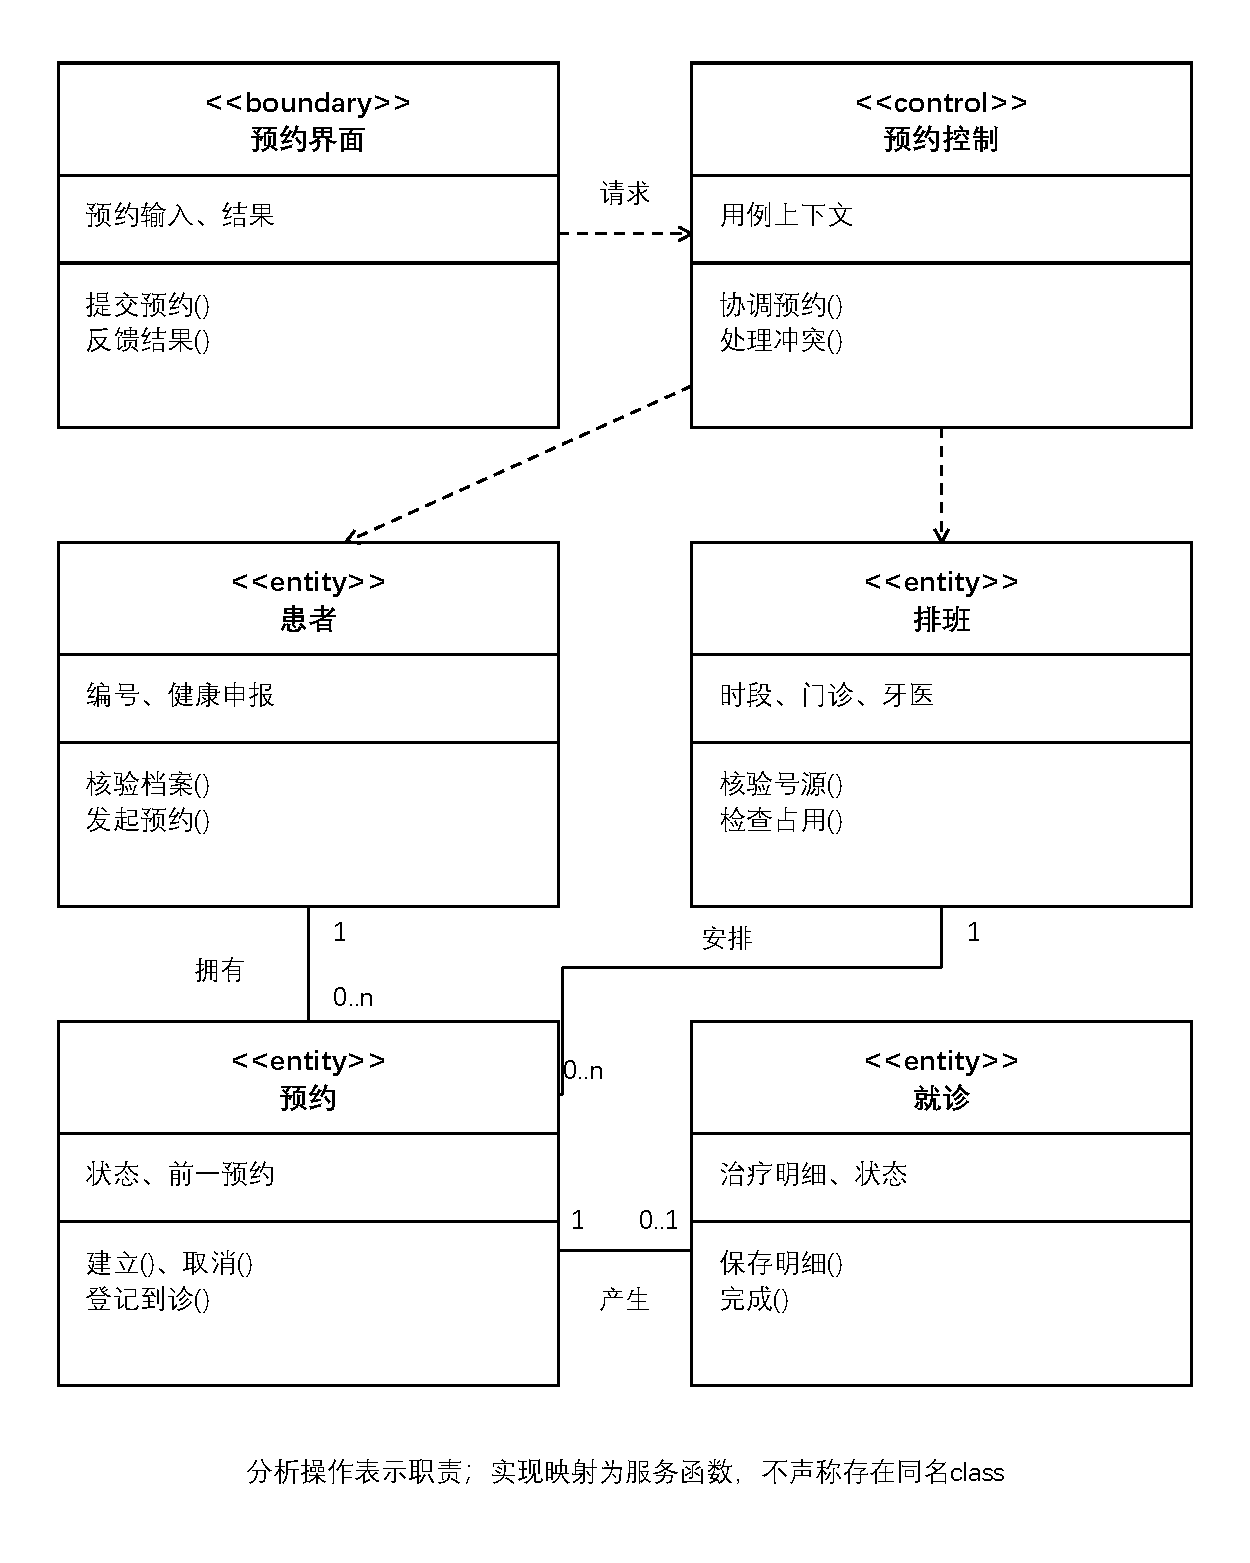
\includegraphics[width=\textwidth]{figures/analysis_classes.pdf}
\caption{预约与诊疗分析类图}\label{analysis_classes}\end{figure}
{\fontsize{10.5pt}{15pt}\selectfont\setlength{\tabcolsep}{0pt}\renewcommand{\arraystretch}{1.08}
\begin{longtable}{@{}p{2.840cm}@{\hspace{0.16cm}}p{6.140cm}@{\hspace{0.16cm}}p{6.140cm}@{}}
\caption{分析责任到实现模块}\\
\toprule
\bfseries \Cell{分析概念} & \bfseries \Cell{主要责任} & \bfseries \Cell{实现映射}\\\midrule
\endfirsthead
\toprule
\bfseries \Cell{分析概念} & \bfseries \Cell{主要责任} & \bfseries \Cell{实现映射}\\\midrule
\endhead
\bottomrule\endlastfoot
\Cell{患者} & \Cell{声明资料、保持身份、维护健康信息与核验来源} & \Cell{patients、patient\_\allowbreak{}allergies；patients.\allowbreak{}js}\\[3pt]
\Cell{排班及预约} & \Cell{校验有效资源、时间冲突、预约状态转换} & \Cell{schedules、appointments；appointments.\allowbreak{}js}\\[3pt]
\Cell{就诊与治疗明细} & \Cell{维护治疗数量及价格快照，完成后冻结} & \Cell{visits、visit\_\allowbreak{}lines；clinical.\allowbreak{}js}\\[3pt]
\Cell{结算与账簿} & \Cell{形成唯一开单，核对原款与应收，追加流水} & \Cell{settlements、payments、refunds；finance.\allowbreak{}js}\\[3pt]
\Cell{归并控制} & \Cell{校验身份冲突并迁移引用、撤销会话} & \Cell{patient-merge.\allowbreak{}js、patient\_\allowbreak{}aliases}\\[3pt]
\Cell{账号控制} & \Cell{在职状态、归属、有效管理者和恢复规则} & \Cell{accounts.\allowbreak{}js、users、password\_\allowbreak{}reset\_\allowbreak{}tokens}\\[3pt]
\end{longtable}
}
分析模型使用对象和操作表达责任，当前JavaScript源码采用函数式业务服务与Repository实现这些责任，没有把图上的分析类名称虚称为源码中实际存在的class。课程物理页313—320强调通过消息完成责任分配，因此图中每个请求都有明确接收对象，不能把箭头只解释为数据流。\par
\subsection{关键分析与设计交互}
\begin{figure}[H]\centering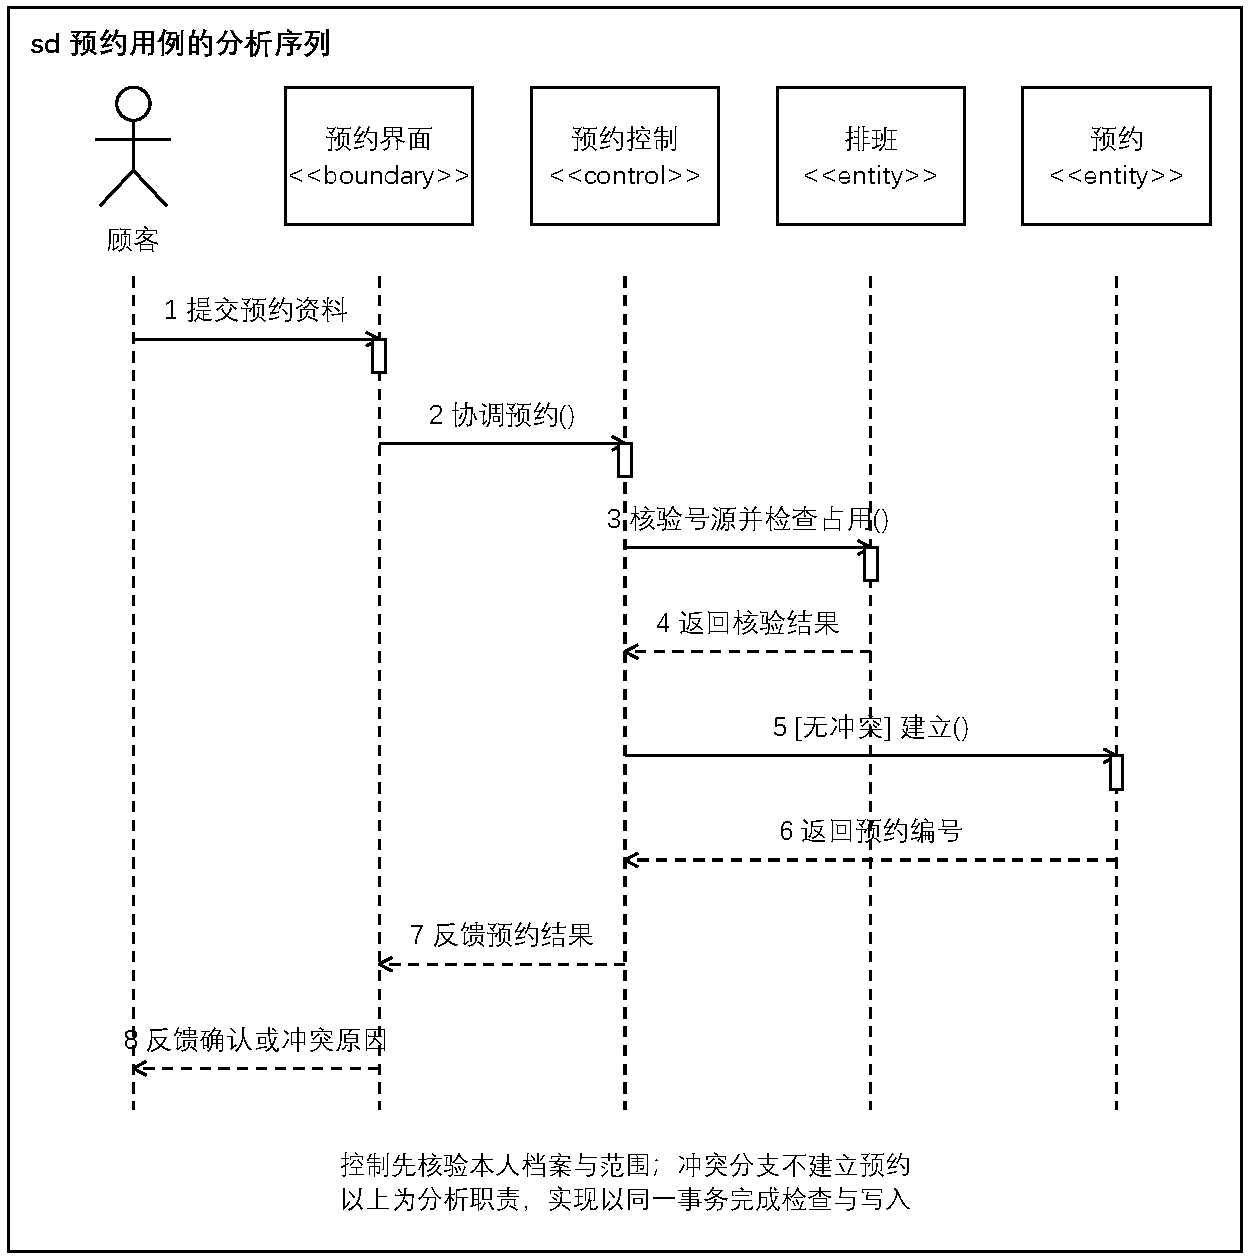
\includegraphics[width=\textwidth]{figures/analysis_booking.pdf}
\caption{预约用例的分析序列}\label{analysis_booking}\end{figure}
预约控制根据当前会话确定患者范围，要求排班提供有效时段和容量信息，并由预约集合判断医生及患者的重叠占用。成功后才建立预约；若检查或保存失败，同一事务回滚。界面只接收确认或冲突结果，不自行以本页数组推断全库可用性。\par
\begin{figure}[H]\centering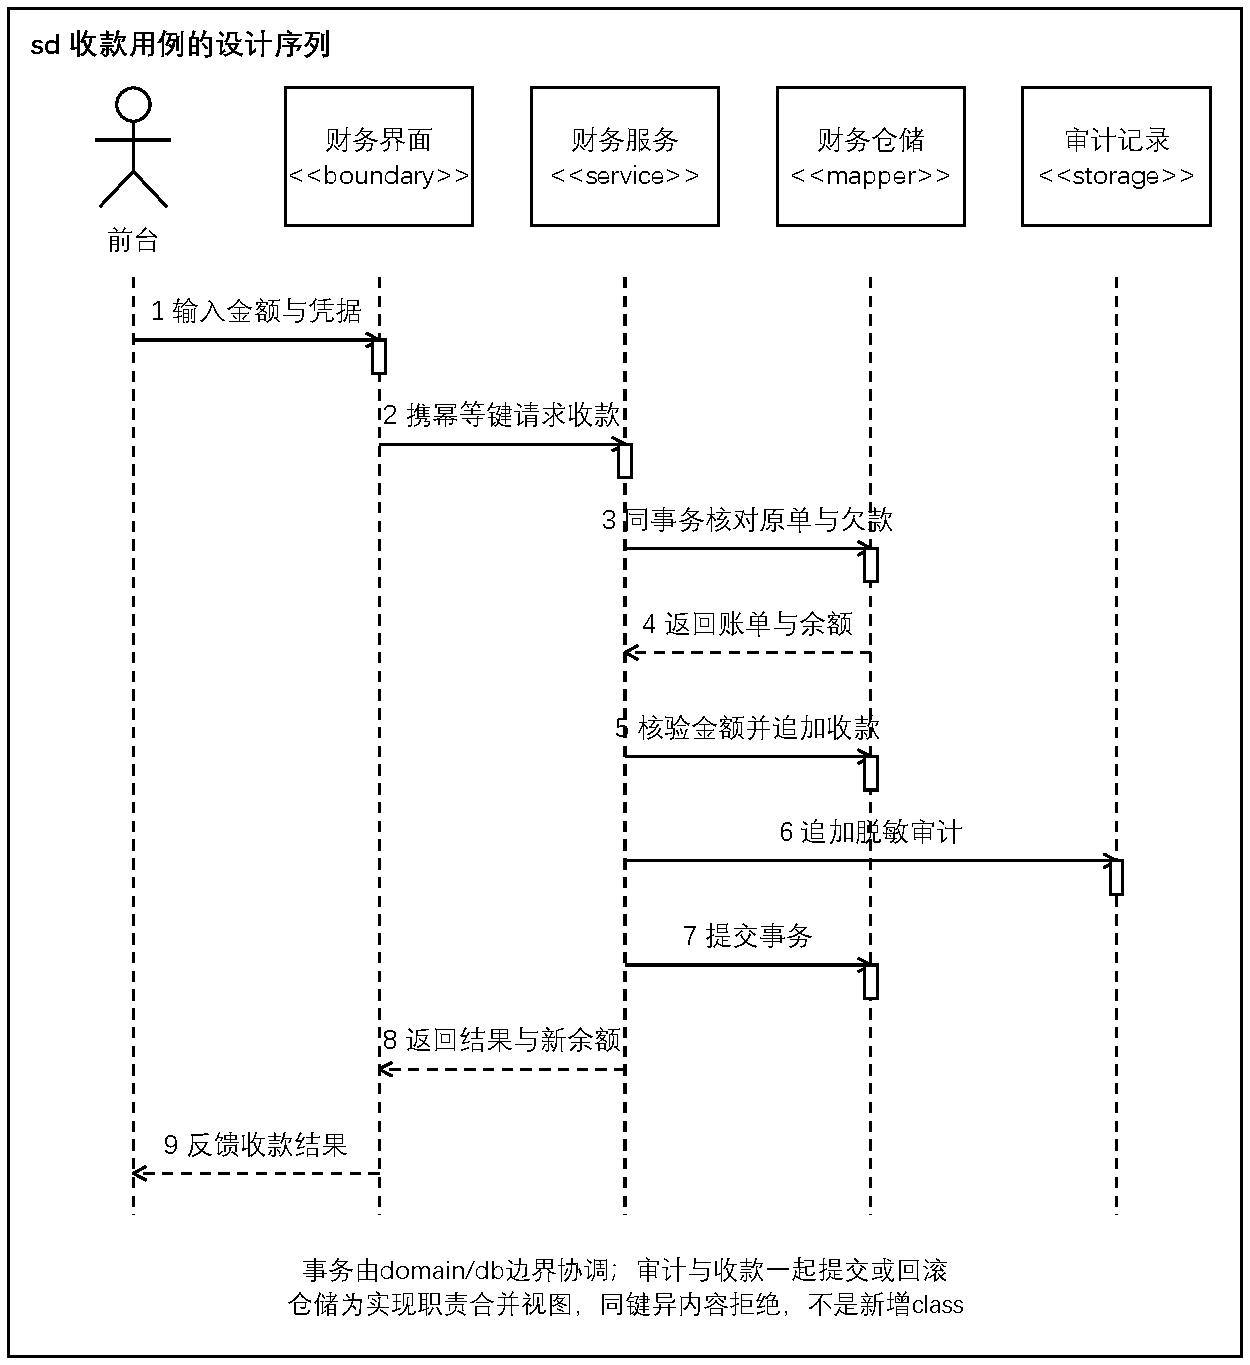
\includegraphics[width=\textwidth]{figures/analysis_finance.pdf}
\caption{收款用例的设计序列}\label{analysis_finance}\end{figure}
财务设计序列进一步加入事务仓储与审计责任。原单的应收、已收和已退共同决定本次可收金额；幂等结果与新流水在同一事务内保存，避免网络重试生成第二笔款项。审计由独立机制留痕，日志中不保存口令或恢复原始凭证。\par
\subsection{对象状态与不变式}
\begin{figure}[H]\centering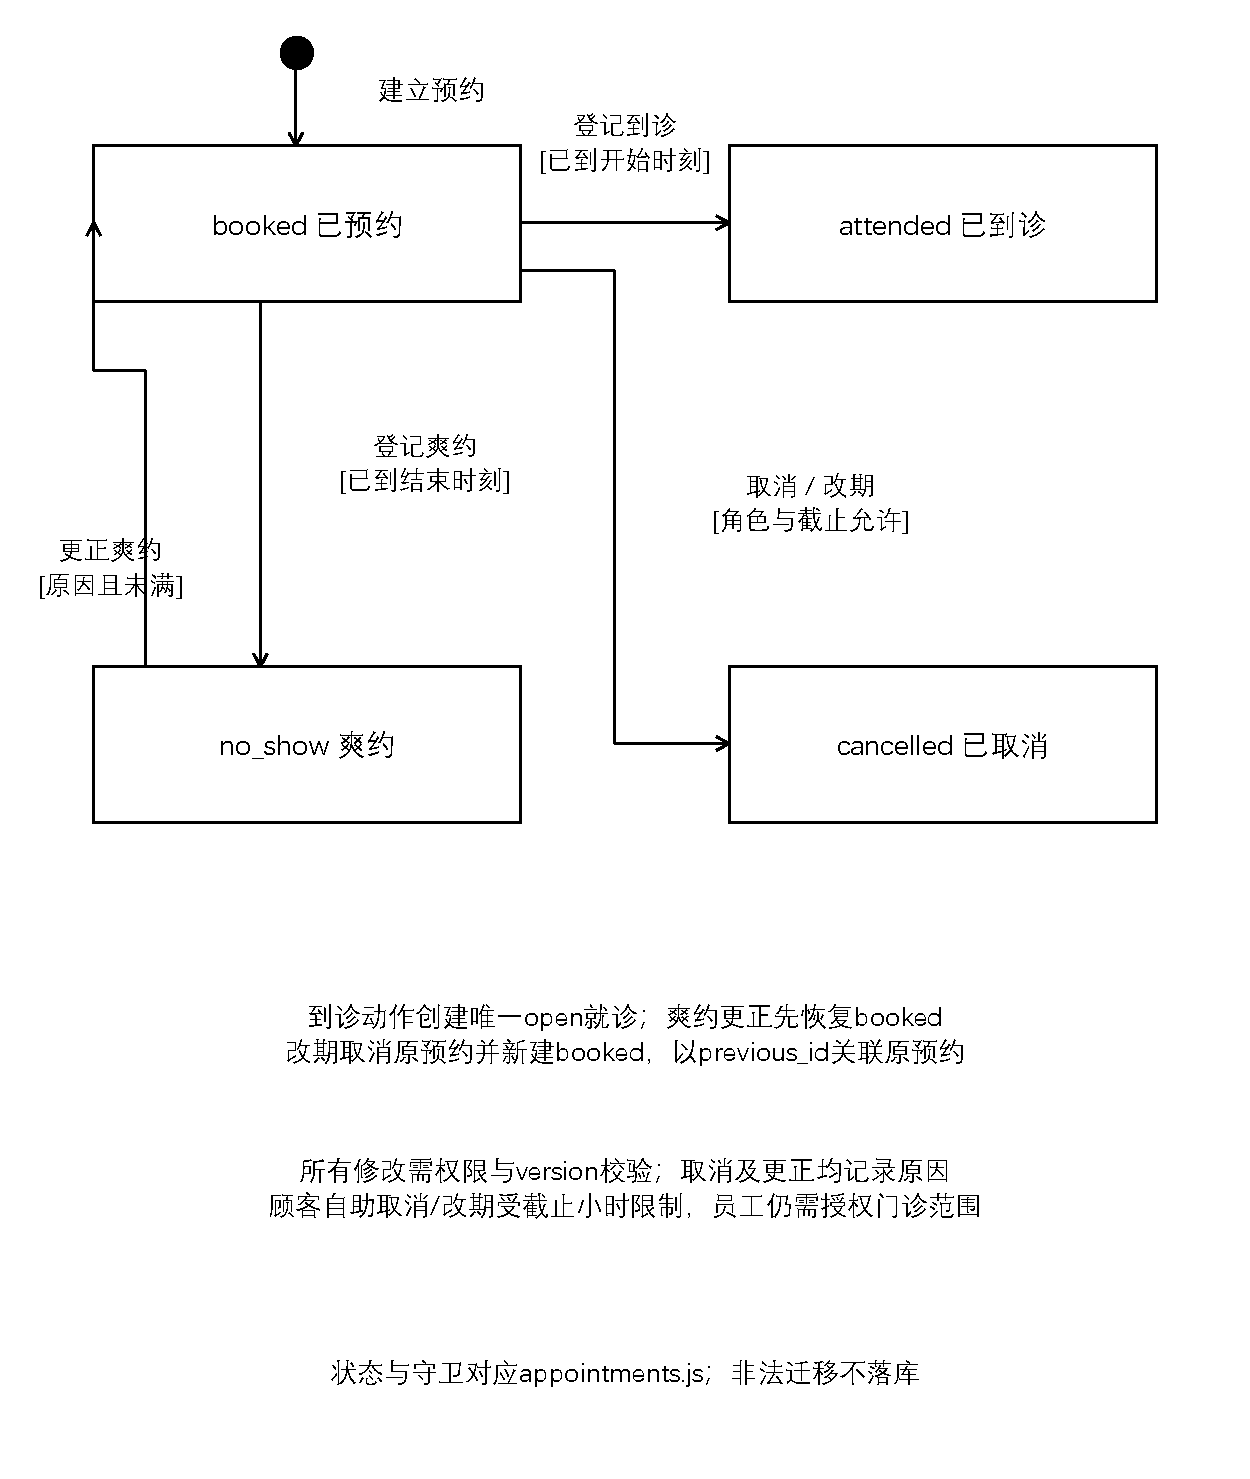
\includegraphics[width=\textwidth]{figures/appointment_states.pdf}
\caption{预约状态机}\label{appointment_states}\end{figure}
\begin{figure}[H]\centering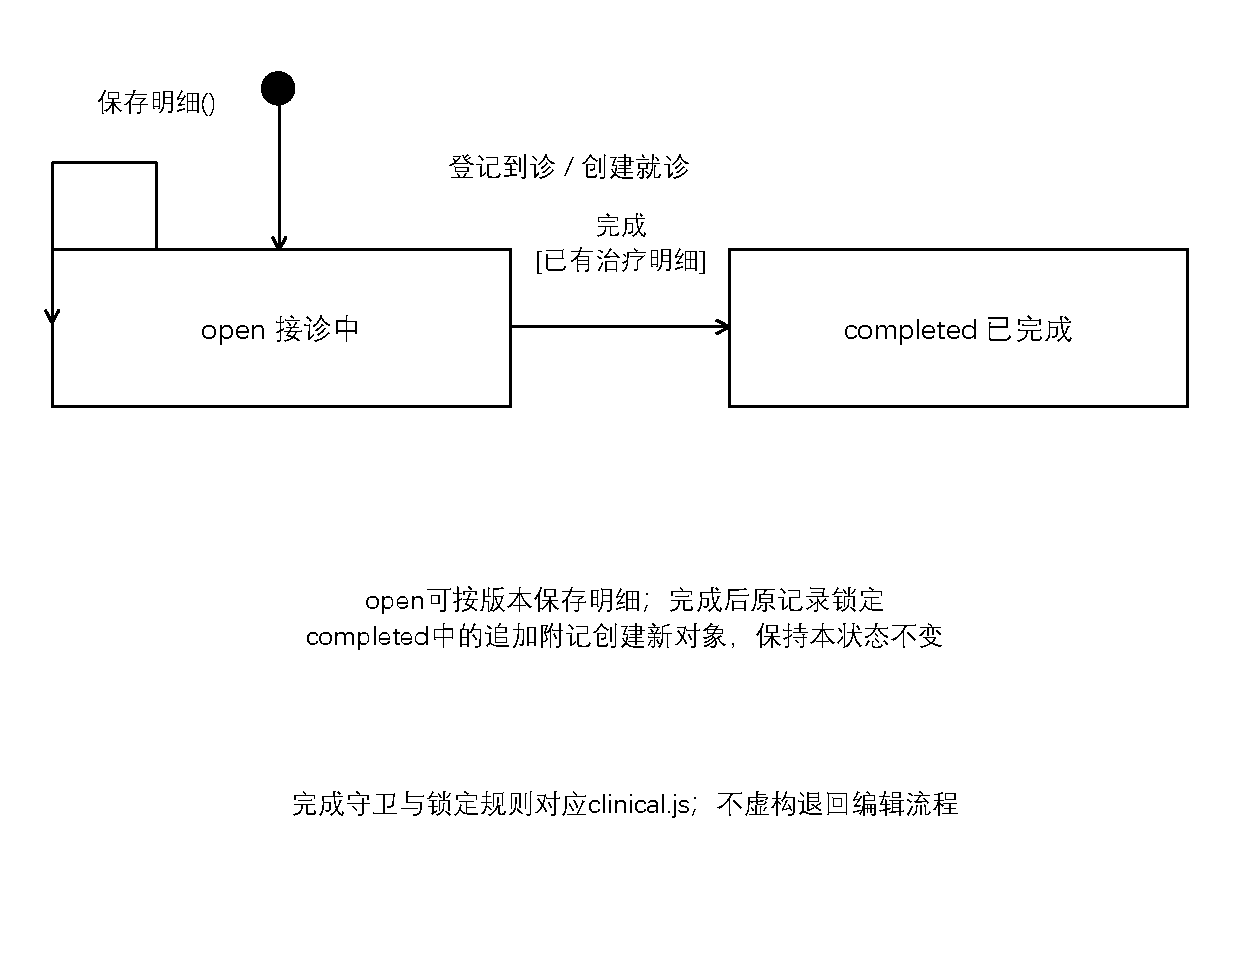
\includegraphics[width=\textwidth]{figures/clinical_states.pdf}
\caption{诊疗记录状态机}\label{clinical_states}\end{figure}
\begin{figure}[H]\centering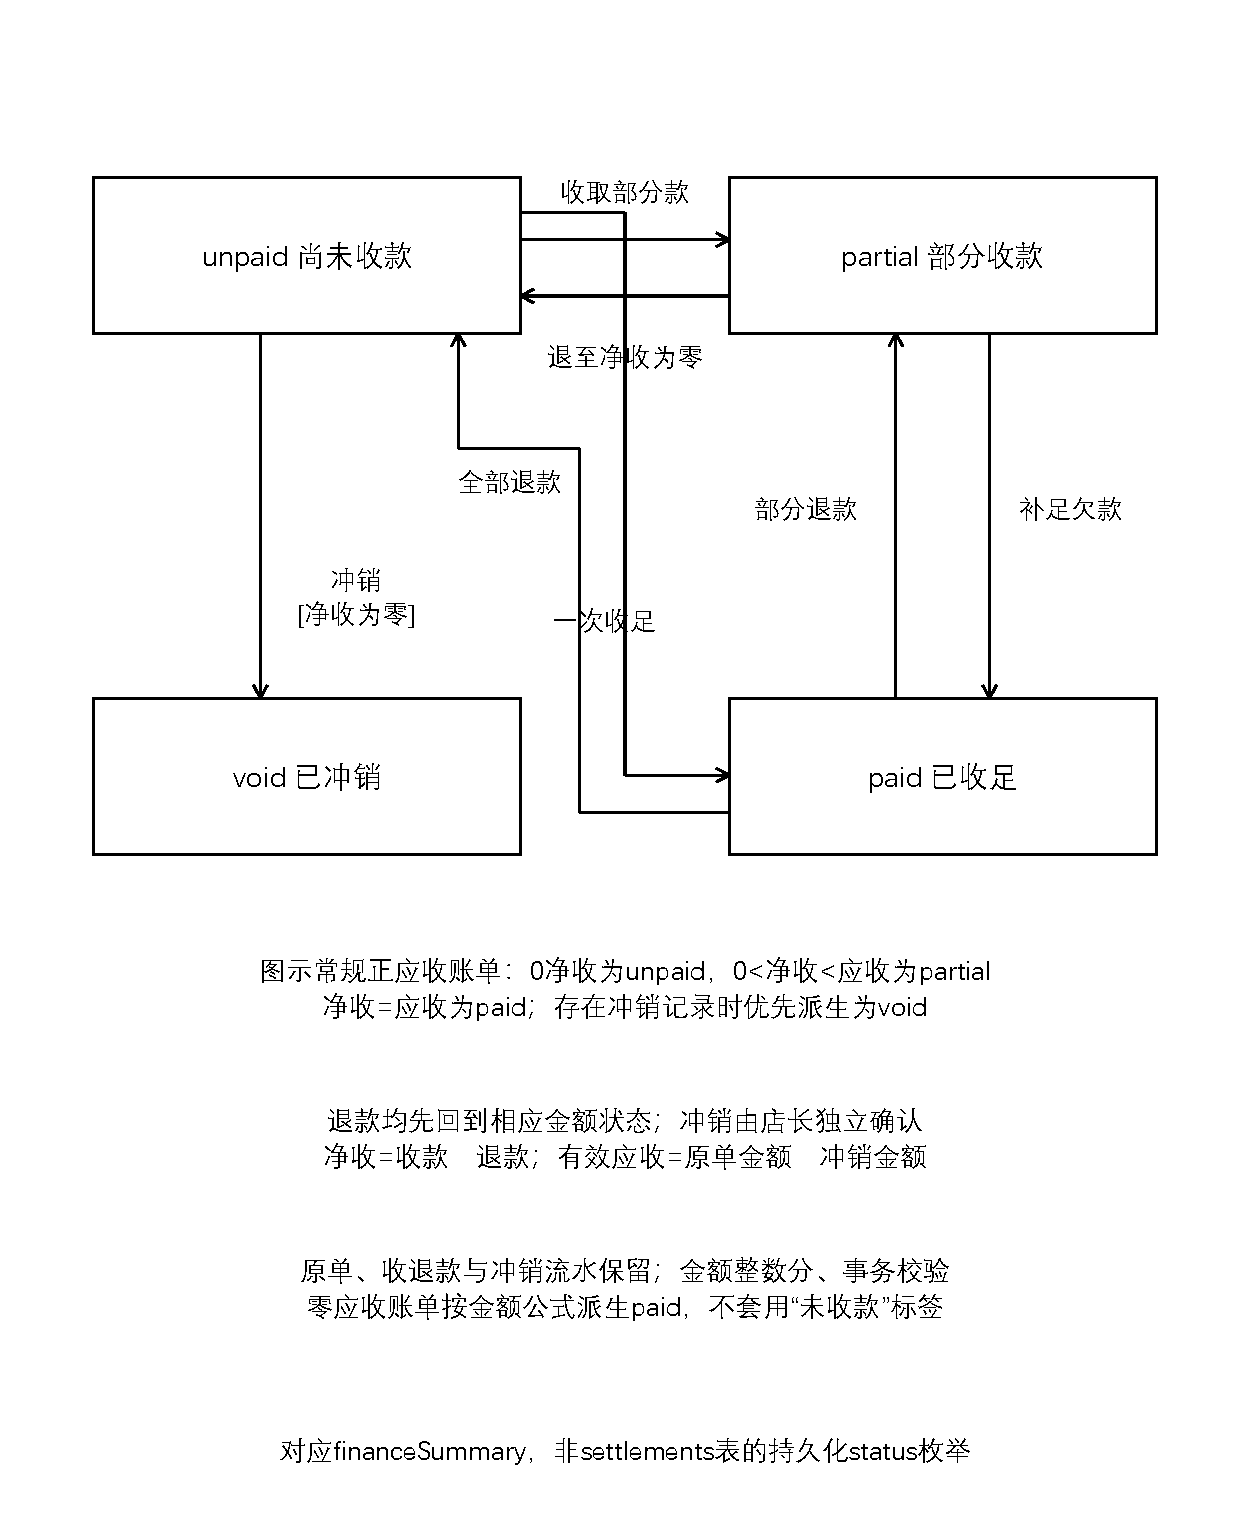
\includegraphics[width=\textwidth]{figures/financial_states.pdf}
\caption{结算金额派生状态与冲销}\label{financial_states}\end{figure}
\begin{figure}[H]\centering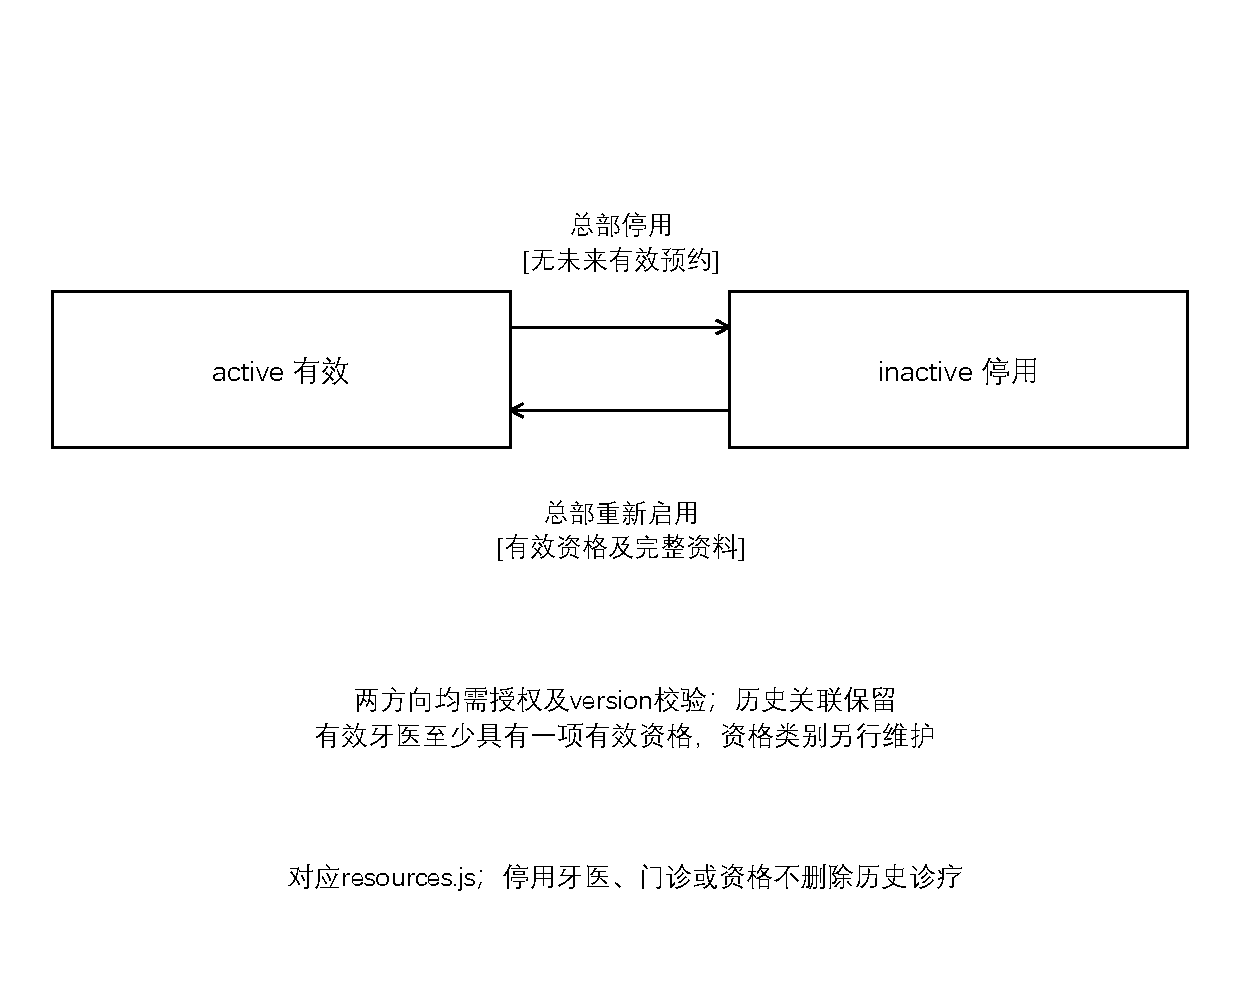
\includegraphics[width=\textwidth]{figures/dentist_states.pdf}
\caption{牙医资源对象状态机}\label{dentist_states}\end{figure}
预约状态是持久化枚举；诊疗仅有open和completed，附记为完成后追加的独立对象。结算的unpaid、partial、paid和void是金额聚合得到的视图状态，settlements没有持久化status字段，不能把派生状态当作物理列。牙医有效性是资源状态，停用不删除历史关联。状态迁移均需符合事件、警戒条件、动作和目标状态，拒绝以页面操作绕开服务端守卫。\par
\subsection{四架构型分析}
\begin{figure}[H]\centering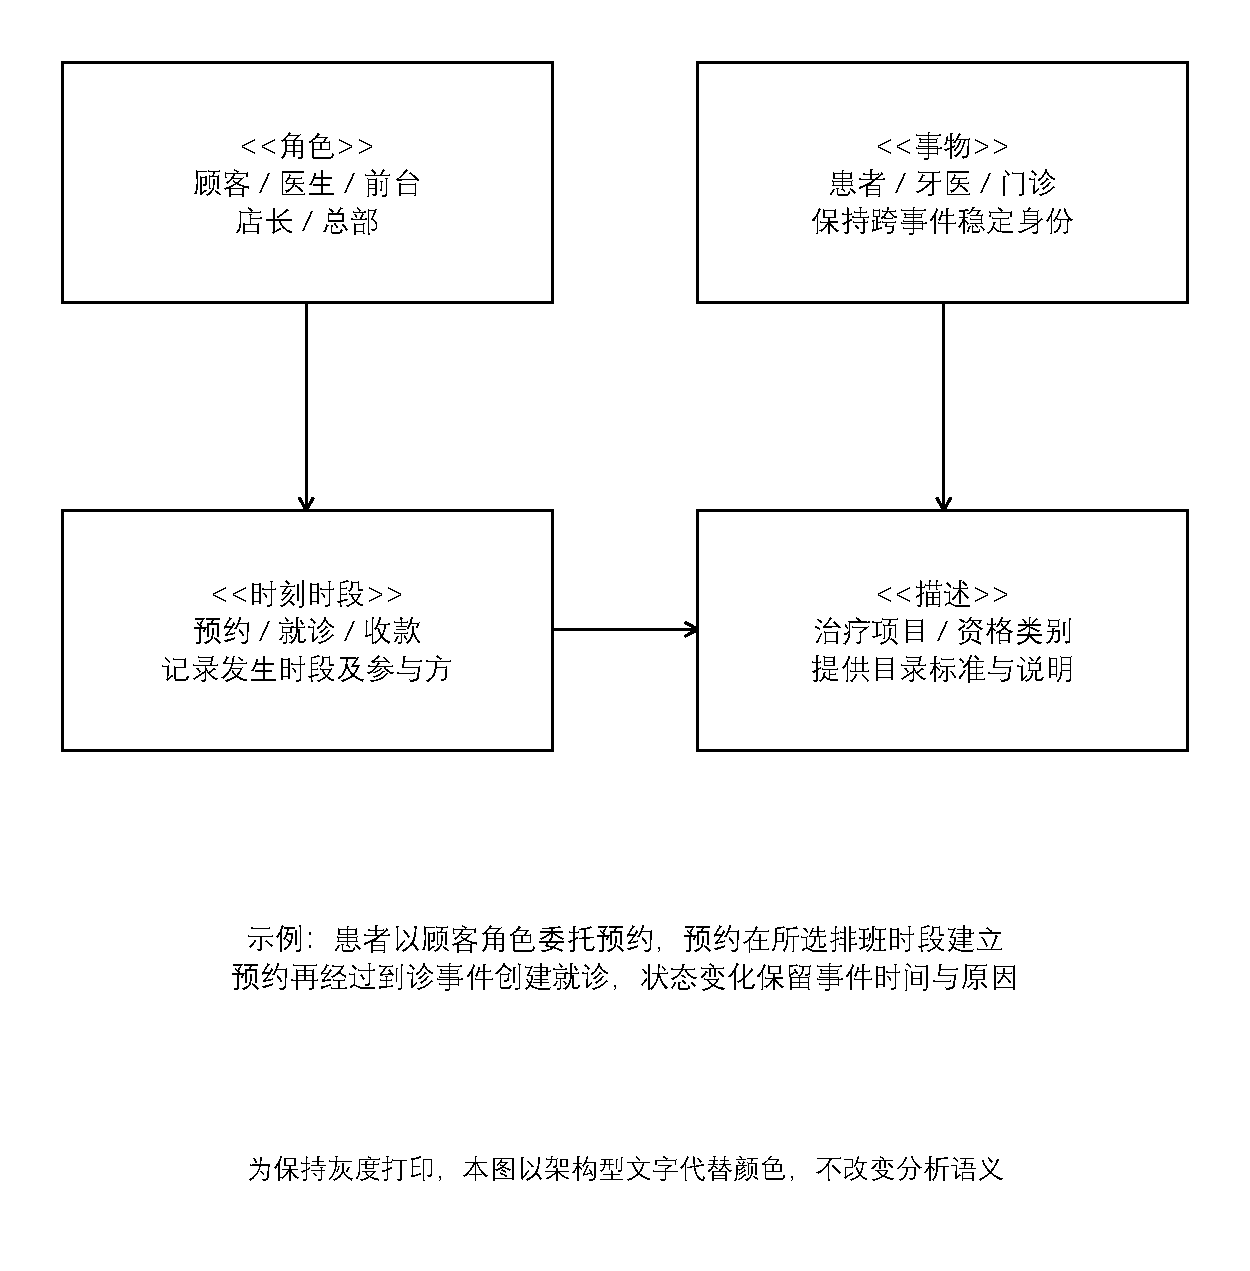
\includegraphics[width=\textwidth]{figures/colored_model.pdf}
\caption{四架构型的职责映射}\label{colored_model}\end{figure}
\begin{figure}[H]\centering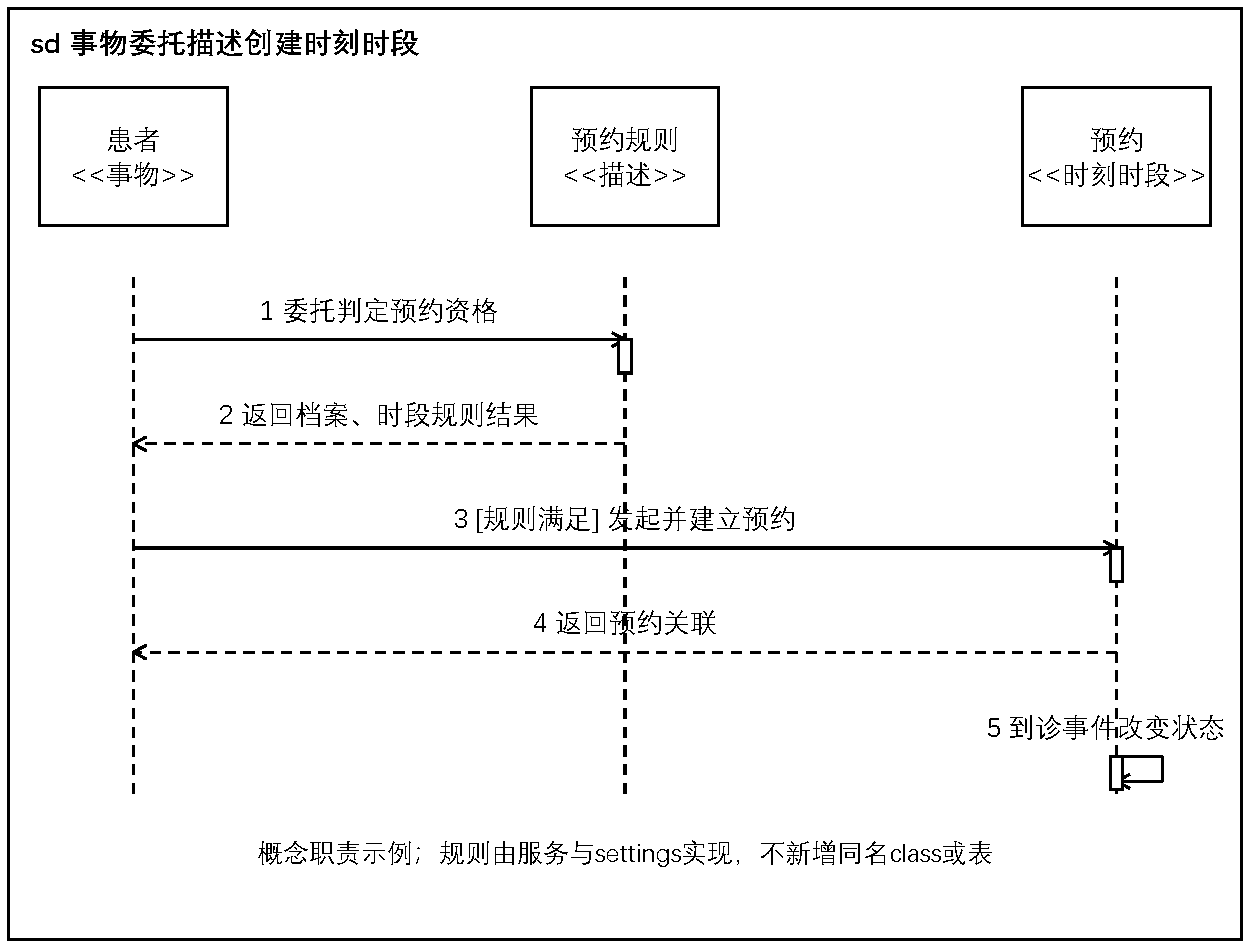
\includegraphics[width=\textwidth]{figures/archetype_sequence.pdf}
\caption{事物委托描述创建时刻时段}\label{archetype_sequence}\end{figure}
按课件物理页385—387的练习，患者、门诊和牙医属于保持身份的事物；顾客、接诊医生等表示参与责任；治疗项目及资格类别提供相对稳定的描述；预约、就诊和收款记录发生的时刻或时段。架构型用于检查职责，不要求为每个标签另建表。患者委托预约规则判断可用时段，规则满足后创建预约，到诊事件再触发状态变化；实现中该规则分配在业务服务与设置中。\par
\Needspace{9\baselineskip}
\section{总体架构与表示层设计}
\subsection{分层架构与源码组织}
\begin{figure}[H]\centering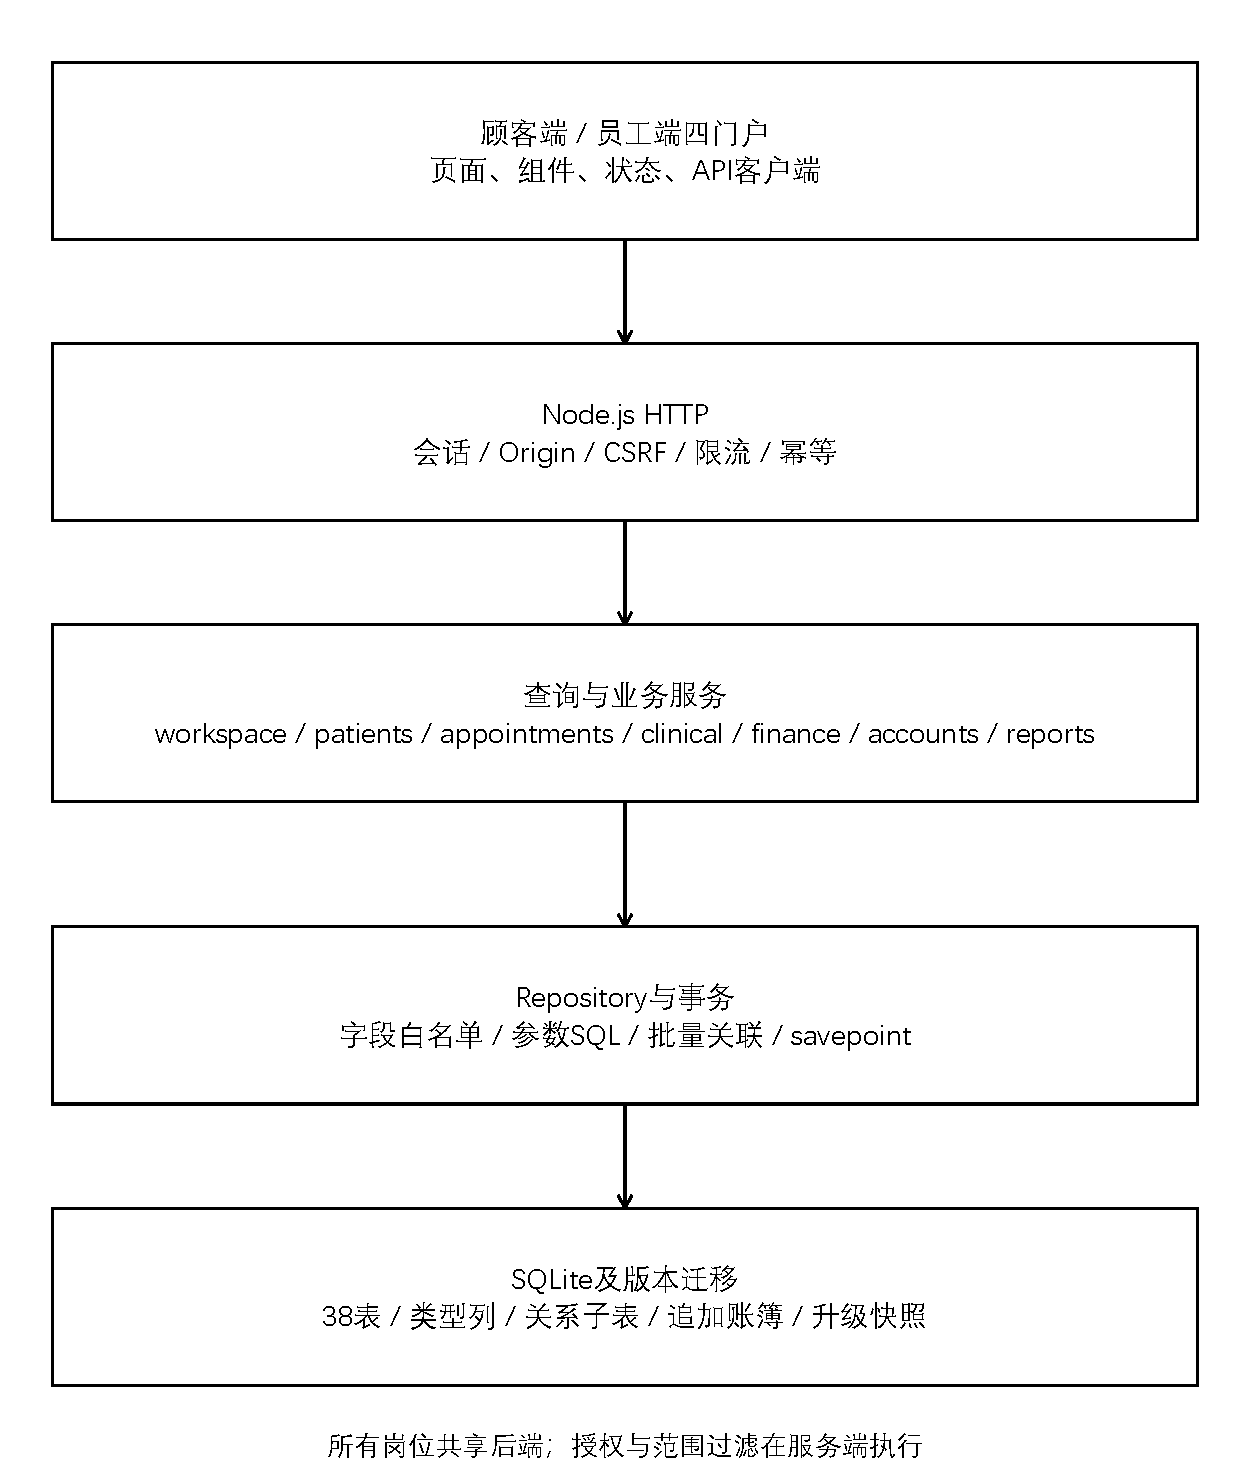
\includegraphics[width=\textwidth]{figures/architecture.pdf}
\caption{应用分层与模块依赖}\label{architecture}\end{figure}
{\fontsize{10.5pt}{15pt}\selectfont\setlength{\tabcolsep}{0pt}\renewcommand{\arraystretch}{1.08}
\begin{longtable}{@{}p{3.940cm}@{\hspace{0.16cm}}p{6.540cm}@{\hspace{0.16cm}}p{4.640cm}@{}}
\caption{源码模块与依赖边界}\\
\toprule
\bfseries \Cell{路径} & \bfseries \Cell{职责} & \bfseries \Cell{依赖限制}\\\midrule
\endfirsthead
\toprule
\bfseries \Cell{路径} & \bfseries \Cell{职责} & \bfseries \Cell{依赖限制}\\\midrule
\endhead
\bottomrule\endlastfoot
\Cell{public/\allowbreak{}app.\allowbreak{}js、js/\allowbreak{}core} & \Cell{入口、路由、会话、API与状态} & \Cell{不在页面内硬编码服务端权限}\\[3pt]
\Cell{public/\allowbreak{}js/\allowbreak{}components、pages} & \Cell{外壳、弹窗、分页与业务页面} & \Cell{通过统一API读写，不直接拼接数据库结构}\\[3pt]
\Cell{public/\allowbreak{}css} & \Cell{布局、组件、岗位主题、响应式及无障碍} & \Cell{通过构建生成styles.\allowbreak{}css，不连续追加主题覆盖}\\[3pt]
\Cell{server/\allowbreak{}index.\allowbreak{}js、http} & \Cell{请求路由、Cookie、CSRF、限流、幂等与配置校验} & \Cell{业务规则交给服务层}\\[3pt]
\Cell{server/\allowbreak{}services、policies} & \Cell{分域命令、授权、对象范围和工作区查询} & \Cell{通过明确映射访问数据}\\[3pt]
\Cell{server/\allowbreak{}repositories、db.\allowbreak{}js} & \Cell{参数SQL、类型映射、批量关联和事务} & \Cell{不接受客户端自由表名或列名}\\[3pt]
\Cell{server/\allowbreak{}migrations} & \Cell{版本校验、旧结构转换与升级快照} & \Cell{禁止直接修改已应用迁移绕过校验}\\[3pt]
\end{longtable}
}
前端由25个ES模块承担核心、组件和页面职责，入口只安装路由与事件。后端保留一个HTTP应用，命令经权限、对象范围和事务控制后进入分域服务；读取由workspace执行条件查询、分页和批量关联。该分层减少原大型app.\allowbreak{}js和domain.\allowbreak{}js的职责混杂，但不引入没有业务收益的跨进程调用。\par
\subsection{按页面查询与局部更新}
日常页面调用GET /\allowbreak{}api/\allowbreak{}workspace而不是反复读取整包/\allowbreak{}api/\allowbreak{}state。服务器同时限制角色可见页面与对象范围，默认每页25条、最大100条。患者和账号使用关键词查询，预约按门诊、牙医、状态及日期窗口筛选；首页统计由SQL聚合，不从当前页样本推算总量。\par
列表更新保留导航和用户菜单，只替换业务主区。日历按所选日或周分批读取整个日期窗口，不能将第一页25条误认为该周全部预约。待开单诊疗、营业日日结和时段选择器使用独立分页偏移，避免一个列表翻页影响另一个业务对象。\par
\Needspace{7\baselineskip}
\subsection{岗位交互与异常反馈}
{\fontsize{10.5pt}{15pt}\selectfont\setlength{\tabcolsep}{0pt}\renewcommand{\arraystretch}{1.08}
\begin{longtable}{@{}p{2.540cm}@{\hspace{0.16cm}}p{7.440cm}@{\hspace{0.16cm}}p{5.140cm}@{}}
\caption{主要岗位交互}\\
\toprule
\bfseries \Cell{场景} & \bfseries \Cell{主要交互} & \bfseries \Cell{失败反馈}\\\midrule
\endfirsthead
\toprule
\bfseries \Cell{场景} & \bfseries \Cell{主要交互} & \bfseries \Cell{失败反馈}\\\midrule
\endhead
\bottomrule\endlastfoot
\Cell{顾客预约} & \Cell{核对本人资料→选择时段→提交问题与特殊需求→查看预约编号} & \Cell{资料不全回到补全；号源冲突刷新；结果不明保留原请求标识}\\[3pt]
\Cell{前台接待} & \Cell{查询授权患者→核对身份健康申报→登记到诊→核对完成记录→开单收款} & \Cell{未到时段拒绝到诊；超额收款拒绝；跨门诊访问拒绝}\\[3pt]
\Cell{医生接诊} & \Cell{读取本人接诊及相关历史→记录治疗→完成→必要时追加附记} & \Cell{他人写入拒绝；版本冲突刷新；完成记录不重新开放}\\[3pt]
\Cell{店长管理} & \Cell{维护资源与账号→核验患者操作→审核成本→核对来源→确认报告} & \Cell{身份冲突或最后有效店长保护拒绝；来源变化要求重算}\\[3pt]
\end{longtable}
}
页面展示加载、成功和可解释错误状态。每次逻辑写入保留唯一标识；请求超时或网络中断后，不凭按钮再次生成新标识重发，用户核对后可沿原标识重试。恢复码仅在签发成功时展示一次，不能依靠重放读取原始凭证。登录、表单及弹窗保持键盘可操作；响应式布局和减少动态偏好由相应CSS层处理。\par
\Needspace{7\baselineskip}
\subsection{接口契约与错误设计}
{\fontsize{10.5pt}{15pt}\selectfont\setlength{\tabcolsep}{0pt}\renewcommand{\arraystretch}{1.08}
\begin{longtable}{@{}p{4.340cm}@{\hspace{0.16cm}}p{6.140cm}@{\hspace{0.16cm}}p{4.640cm}@{}}
\caption{主要HTTP契约}\\
\toprule
\bfseries \Cell{接口} & \bfseries \Cell{请求与返回} & \bfseries \Cell{关键约束}\\\midrule
\endfirsthead
\toprule
\bfseries \Cell{接口} & \bfseries \Cell{请求与返回} & \bfseries \Cell{关键约束}\\\midrule
\endhead
\bottomrule\endlastfoot
\Cell{POST /\allowbreak{}api/\allowbreak{}login} & \Cell{username、password、portal；返回身份与CSRF，签发会话Cookie} & \Cell{入口与角色一致，持久限流}\\[3pt]
\Cell{POST /\allowbreak{}api/\allowbreak{}register} & \Cell{仅customer注册} & \Cell{规范化电话已有档案则转机构核验绑定}\\[3pt]
\Cell{GET /\allowbreak{}api/\allowbreak{}workspace} & \Cell{page及筛选、分页；返回授权数据与pagination} & \Cell{数据范围在服务端执行}\\[3pt]
\Cell{POST /\allowbreak{}api/\allowbreak{}command} & \Cell{type、payload、版本和幂等键} & \Cell{CSRF、角色、范围、状态及事务}\\[3pt]
\Cell{POST /\allowbreak{}api/\allowbreak{}password-recovery/\allowbreak{}request} & \Cell{username与portal；统一回应} & \Cell{不能以回应判断账号存在}\\[3pt]
\Cell{POST /\allowbreak{}api/\allowbreak{}password-recovery/\allowbreak{}consume} & \Cell{token与newPassword} & \Cell{过期或重复消费拒绝，撤销旧会话}\\[3pt]
\Cell{GET /\allowbreak{}api/\allowbreak{}backup} & \Cell{店长业务JSON导出} & \Cell{包含业务流水，不含凭证，不能用于SQLite完整恢复}\\[3pt]
\Cell{GET /\allowbreak{}api/\allowbreak{}health} & \Cell{服务版本及数据库连接状态} & \Cell{不是全部业务健康的替代验收}\\[3pt]
\end{longtable}
}
POST采用application/\allowbreak{}json，已登录修改携带X-CSRF-Token；普通业务命令携带Idempotency-Key。客户端对象使用camelCase，数据层映射到关系型字段。400表示格式或条件不满足，401表示未登录，403表示越权，409表示版本、状态、冲突或重放内容不一致，429表示限流；服务器错误仅给请求标识，不向浏览器回传SQL、路径或堆栈。\par
\Needspace{9\baselineskip}
\section{数据库设计}
\subsection{概念结构与关系基数}
\begin{figure}[H]\centering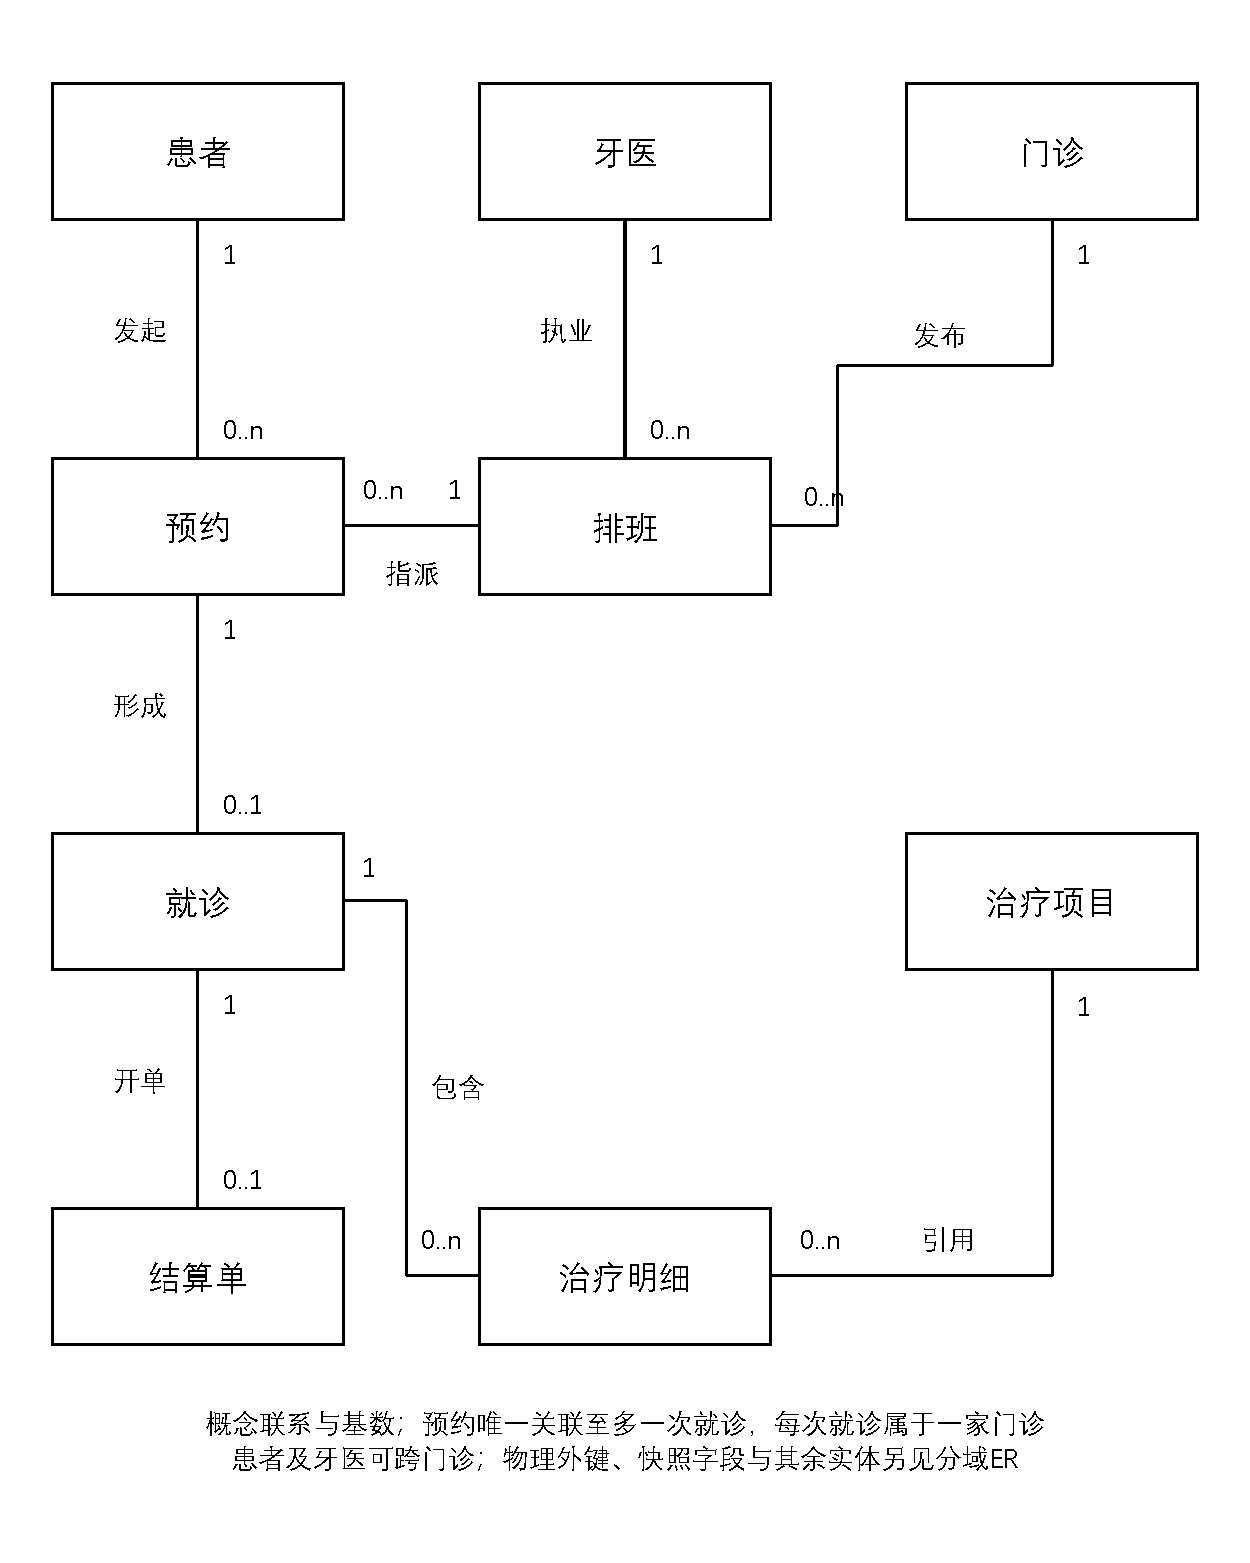
\includegraphics[width=\textwidth]{figures/conceptual_er.pdf}
\caption{核心业务概念ER图}\label{conceptual_er}\end{figure}
患者与预约为一对多，预约与就诊为一对零或一，就诊与结算单为一对零或一。一次就诊包含多条治疗明细，每条关联治疗目录并保存当次名称、数量和单价。医生跨门诊服务通过排班和实际预约、就诊表达；患者的门诊访问授权另设关联，不把创建门诊等同于唯一就诊门诊。\par
六幅物理分域ER图覆盖38张表；框内展示主键、主要外键及核心属性，字段全集见附录A。实线表示SQL已声明的外键，虚线表示服务层逻辑引用；跨域外键在节点及数据字典注明，以避免图上交叉线压过文字。多重性按约束解释，含唯一外键时区别一对零或一。\par
\begin{figure}[H]\centering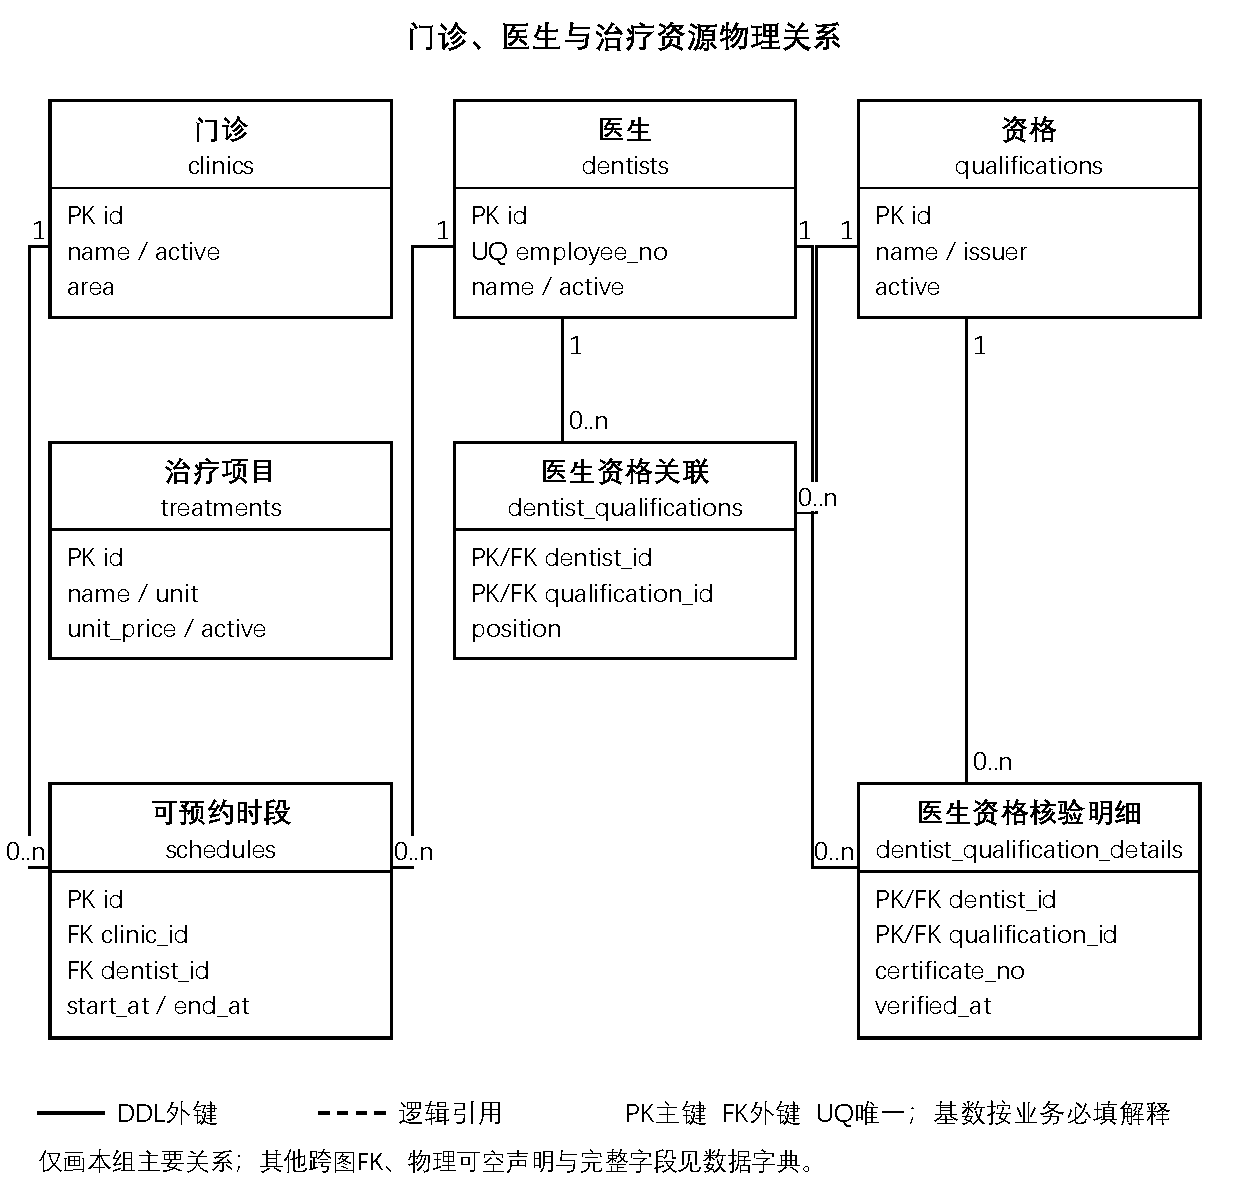
\includegraphics[width=\textwidth]{figures/er01.pdf}
\caption{门诊、医生与治疗资源物理关系}\label{er01}\end{figure}
\begin{figure}[H]\centering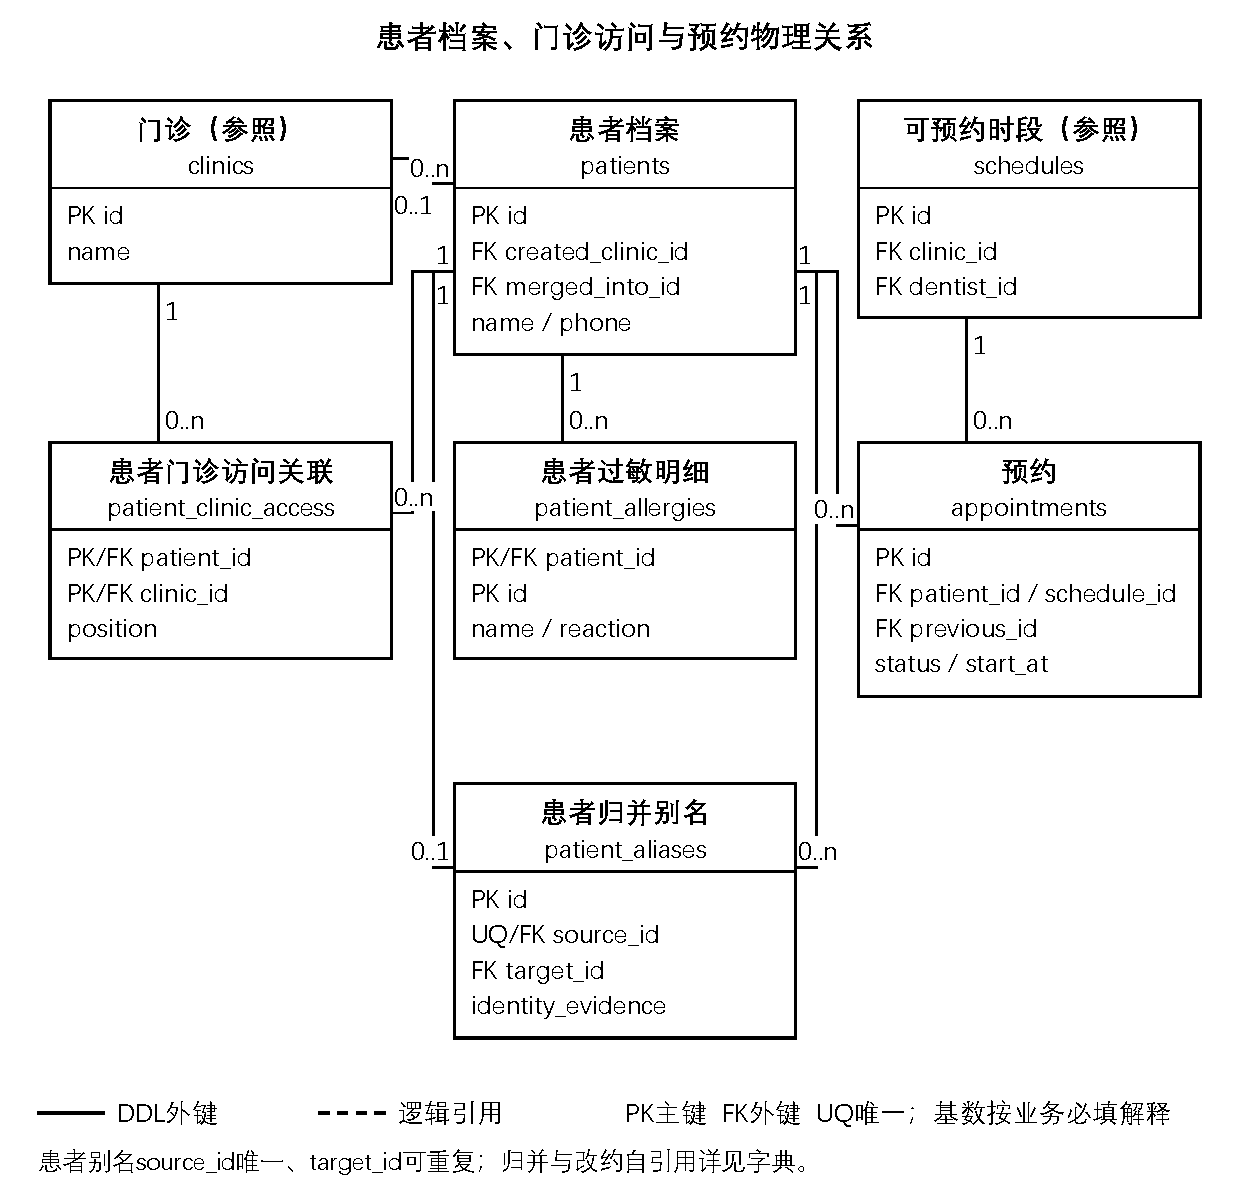
\includegraphics[width=\textwidth]{figures/er02.pdf}
\caption{患者档案、门诊访问与预约物理关系}\label{er02}\end{figure}
\begin{figure}[H]\centering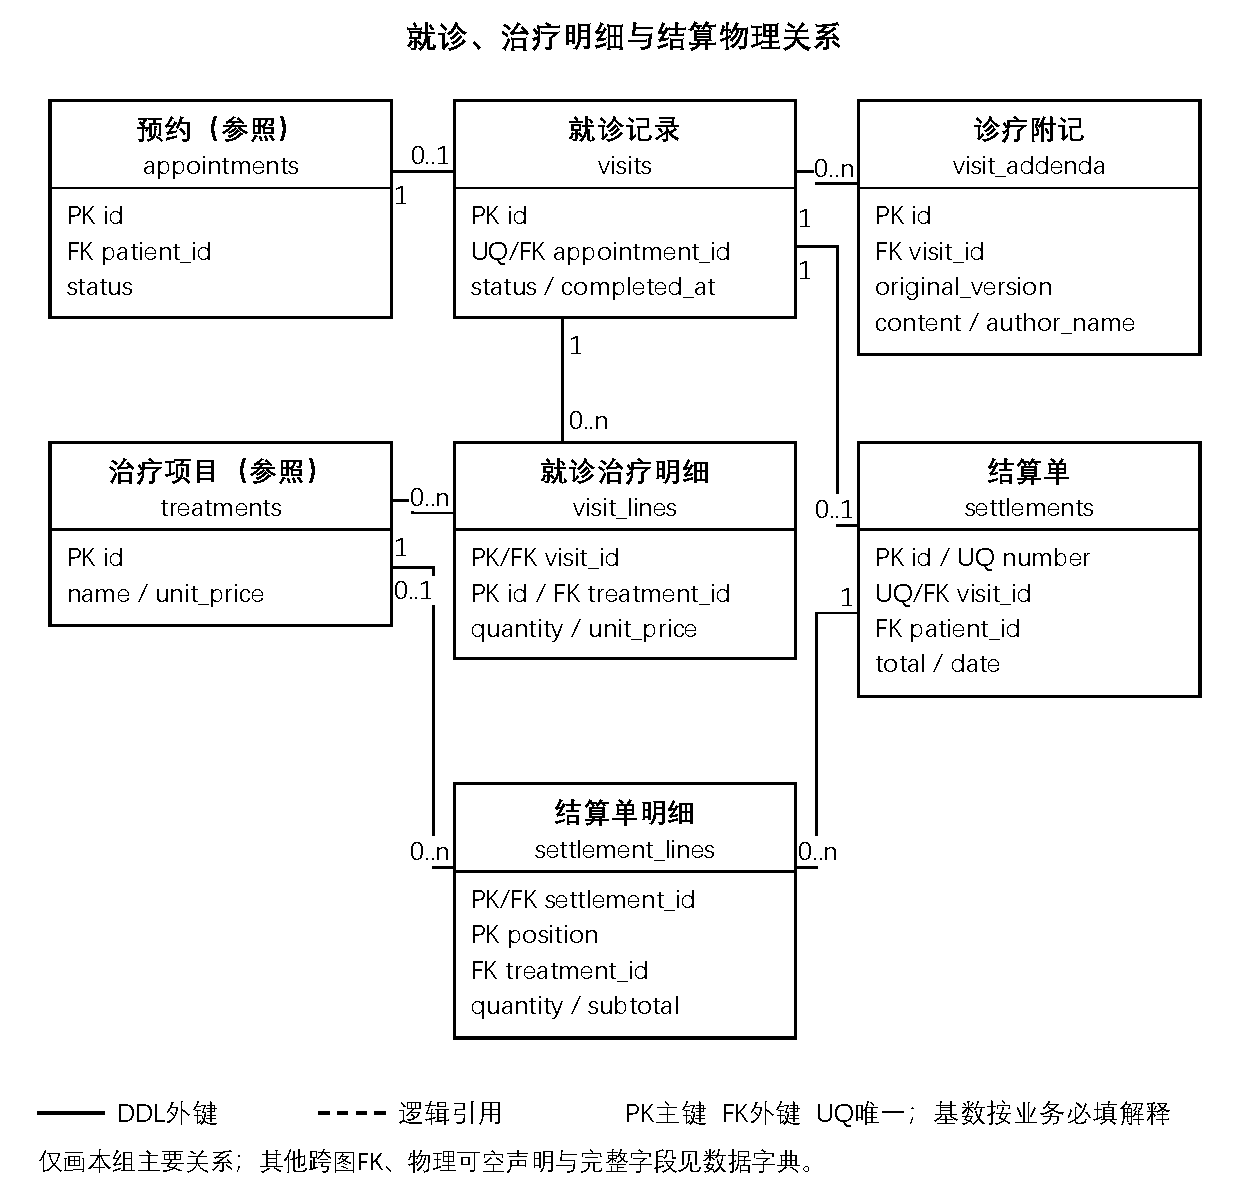
\includegraphics[width=\textwidth]{figures/er03.pdf}
\caption{就诊、治疗明细与结算物理关系}\label{er03}\end{figure}
\begin{figure}[H]\centering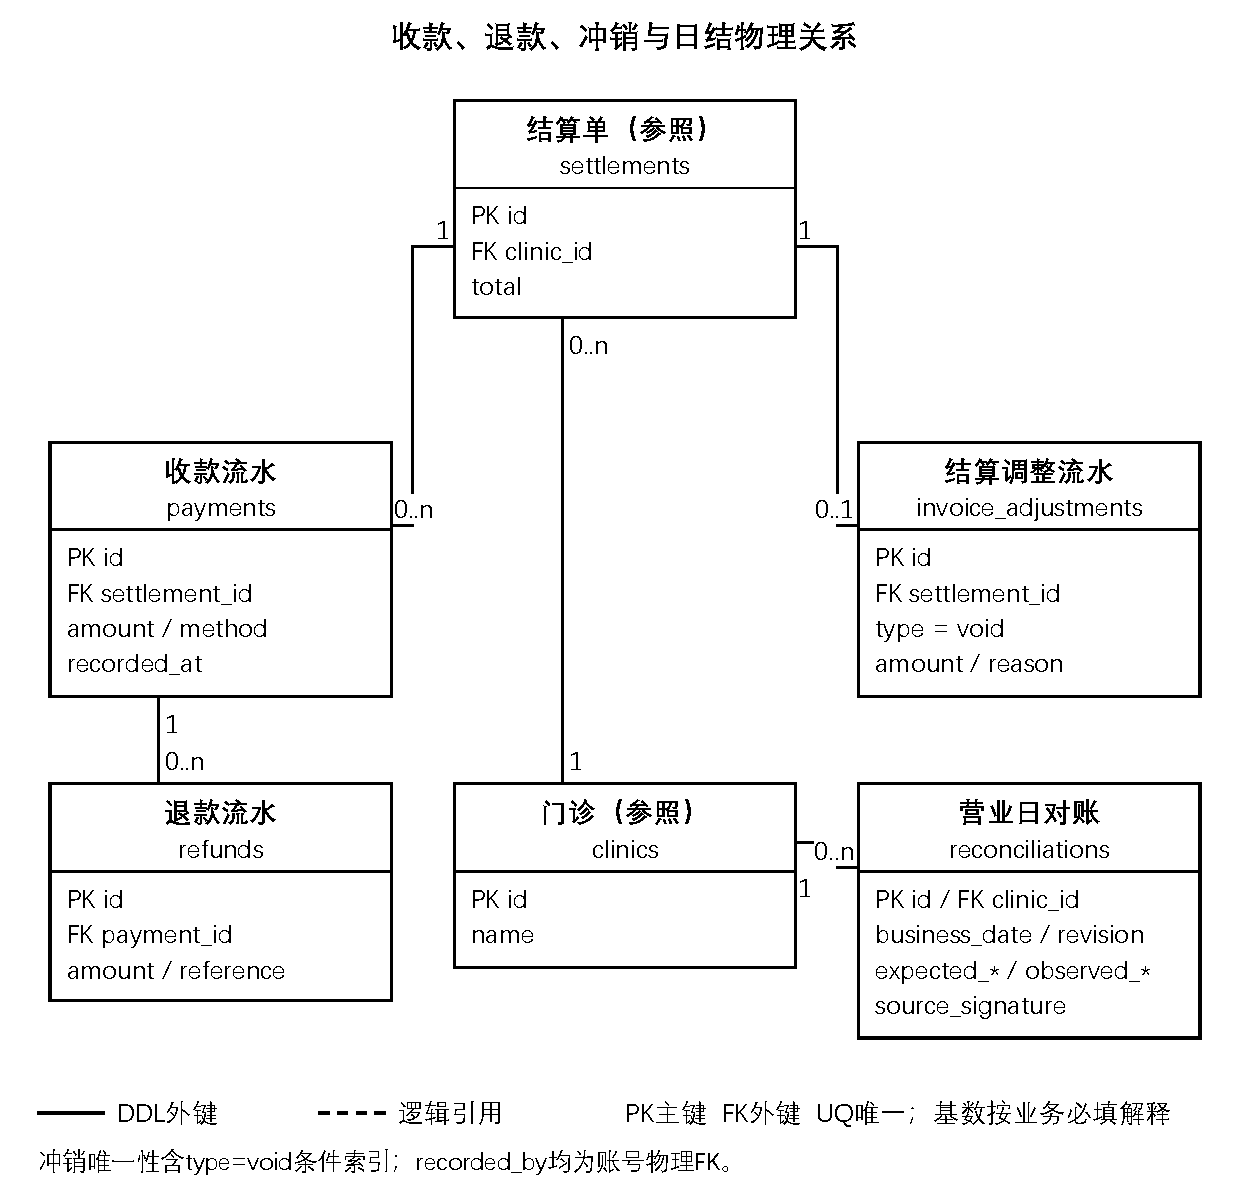
\includegraphics[width=\textwidth]{figures/er04.pdf}
\caption{收款、退款、冲销与日结物理关系}\label{er04}\end{figure}
\begin{figure}[H]\centering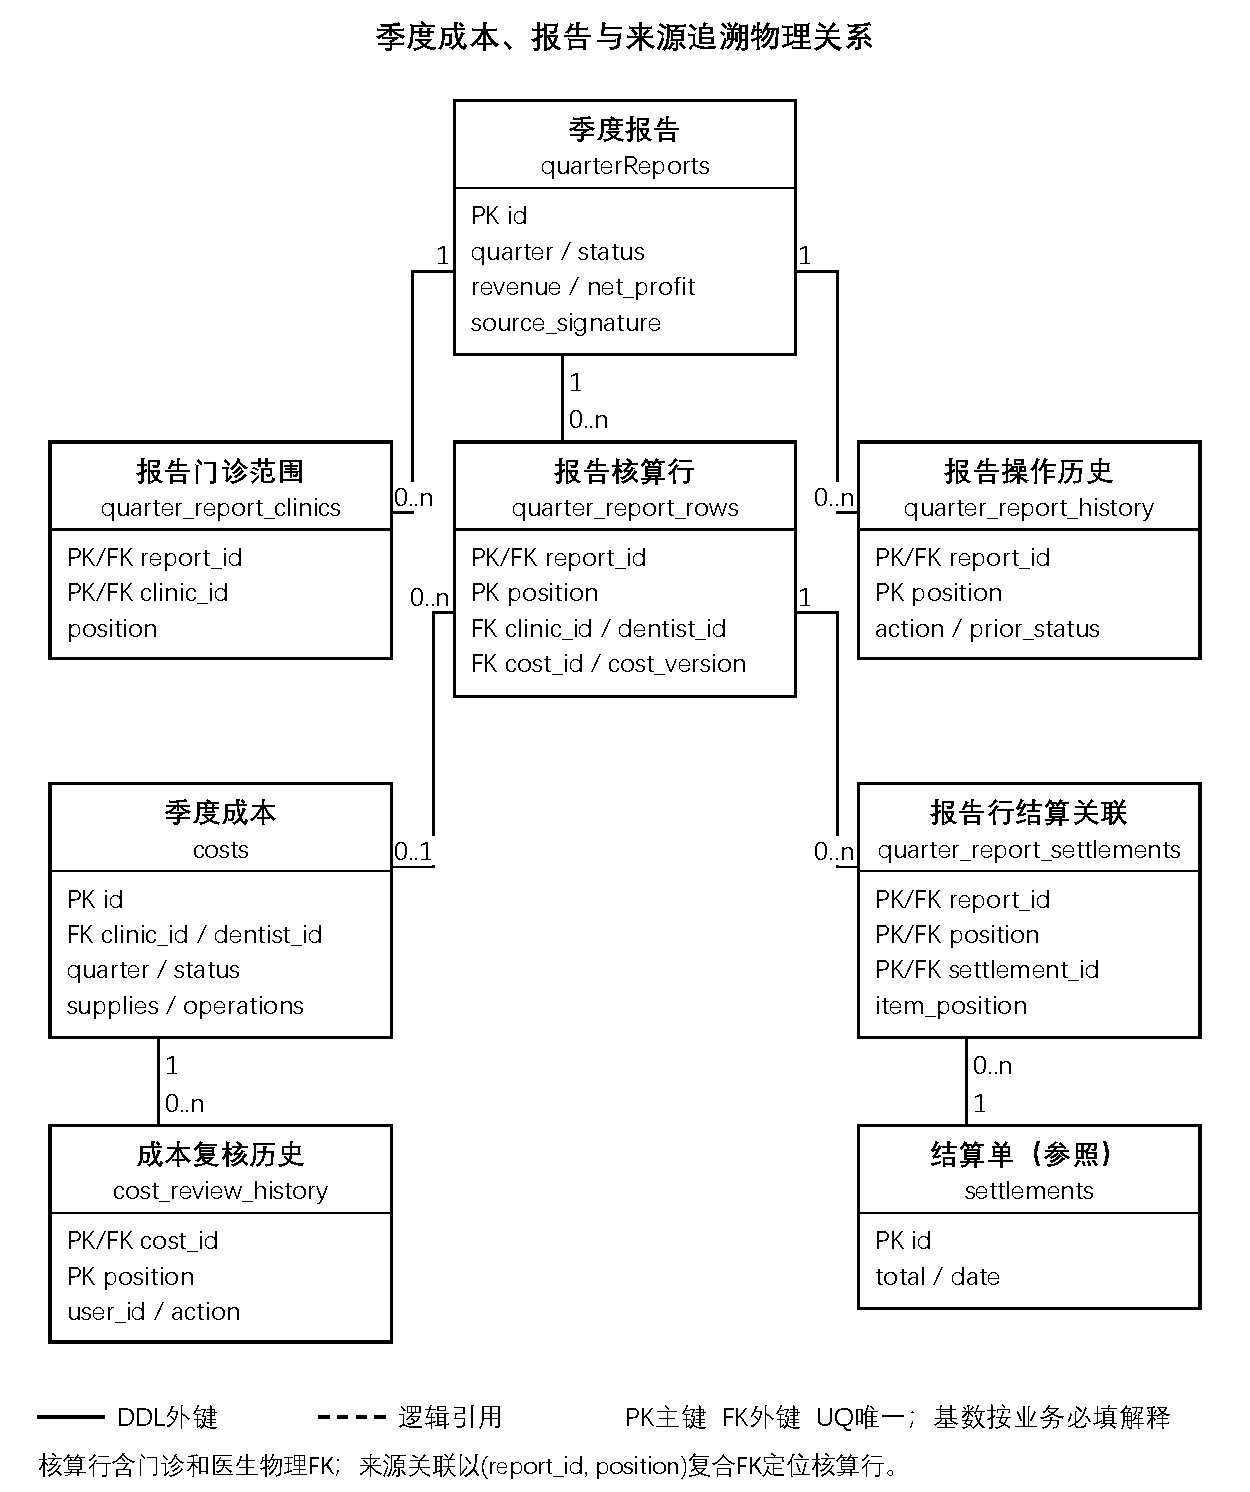
\includegraphics[width=\textwidth]{figures/er05.pdf}
\caption{季度成本、报告与来源追溯物理关系}\label{er05}\end{figure}
\begin{figure}[H]\centering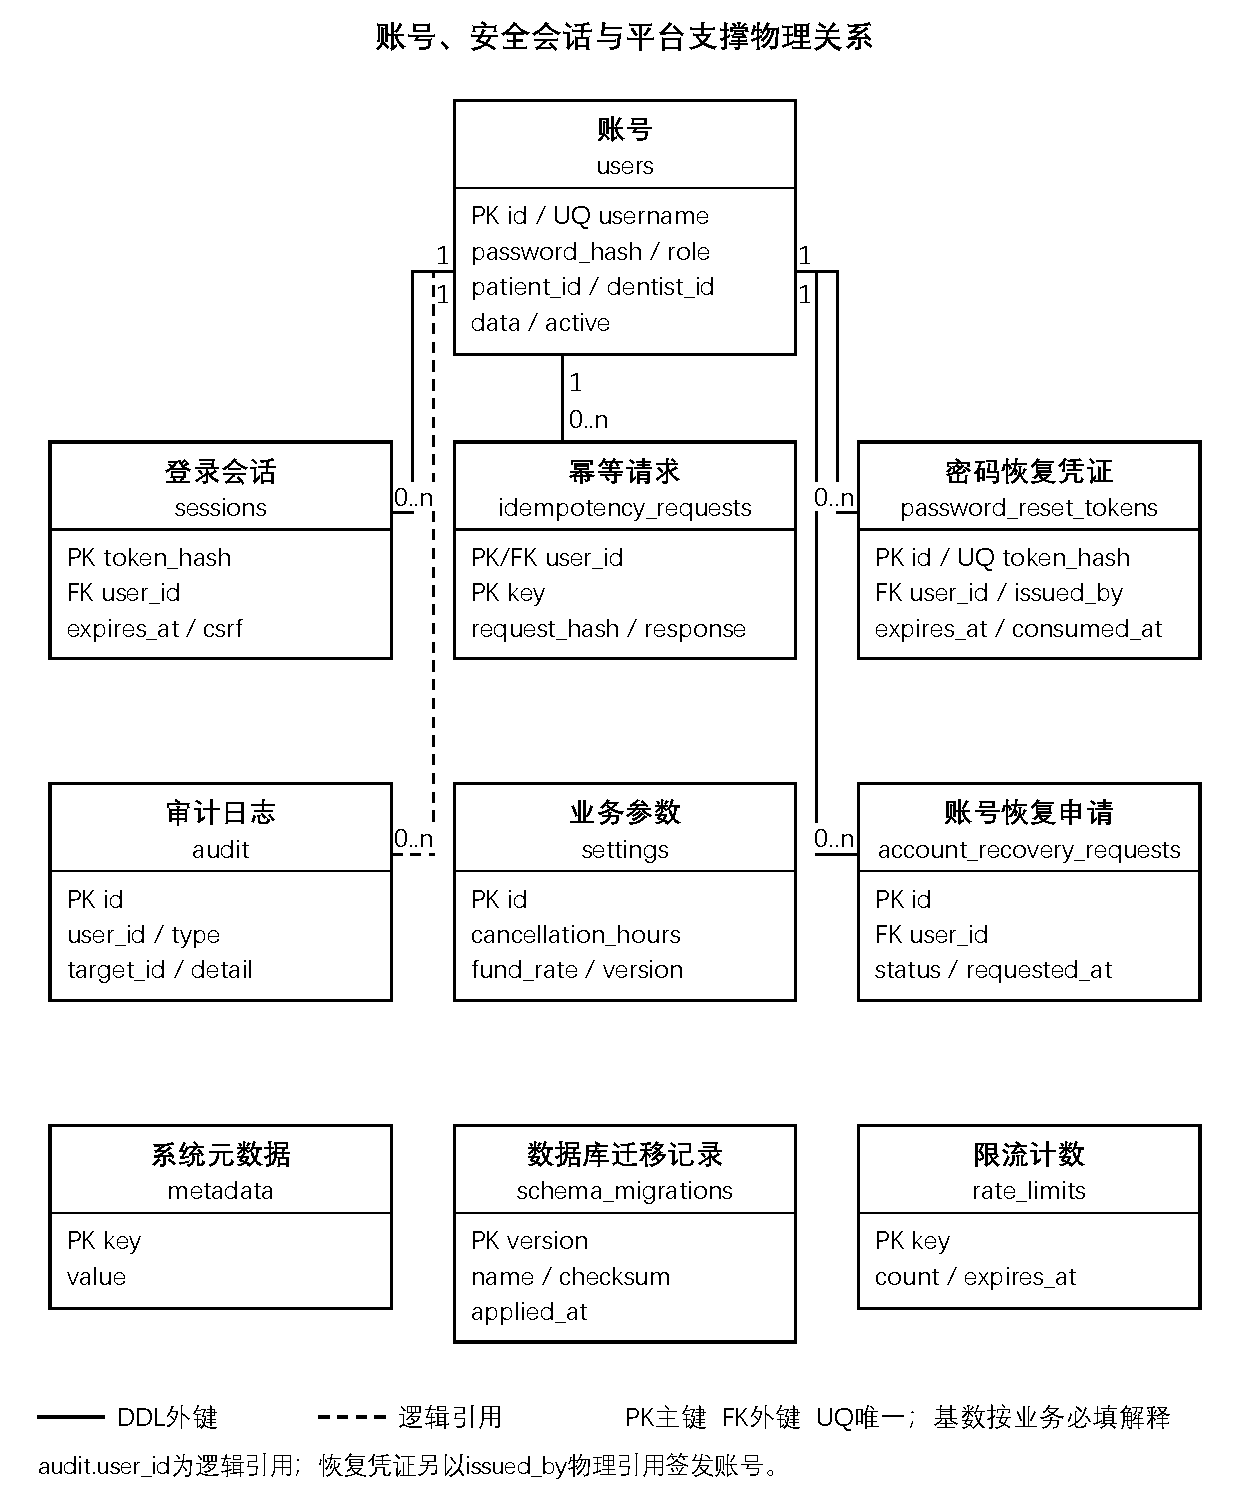
\includegraphics[width=\textwidth]{figures/er06.pdf}
\caption{账号、安全会话与平台支撑物理关系}\label{er06}\end{figure}
\Needspace{7\baselineskip}
\subsection{关系模式与规范化}
{\fontsize{10.5pt}{15pt}\selectfont\setlength{\tabcolsep}{0pt}\renewcommand{\arraystretch}{1.08}
\begin{longtable}{@{}p{2.840cm}@{\hspace{0.16cm}}p{6.040cm}@{\hspace{0.16cm}}p{6.240cm}@{}}
\caption{对象到关系的映射取舍}\\
\toprule
\bfseries \Cell{结构} & \bfseries \Cell{规范化处理} & \bfseries \Cell{保留的快照或兼容选择}\\\midrule
\endfirsthead
\toprule
\bfseries \Cell{结构} & \bfseries \Cell{规范化处理} & \bfseries \Cell{保留的快照或兼容选择}\\\midrule
\endhead
\bottomrule\endlastfoot
\Cell{患者过敏} & \Cell{patient\_\allowbreak{}allergies逐项存储，以患者编号关联} & \Cell{核验时间与来源保留在患者档案}\\[3pt]
\Cell{医生资格} & \Cell{dentist\_\allowbreak{}qualifications表达多对多，details保存核验证书信息} & \Cell{兼容双表共同描述资格，不宣称details已完全消除冗余}\\[3pt]
\Cell{就诊与结算行} & \Cell{聚合根与明细分表，避免一列混装多项治疗} & \Cell{历史名称及单价是有意保留的交易快照}\\[3pt]
\Cell{季度报告} & \Cell{报告头、门诊范围、核算行、来源结算与历史分离} & \Cell{收入及成本合计用于可追溯报告，不随目录变化重写}\\[3pt]
\Cell{账号身份} & \Cell{同步role、name、patient\_\allowbreak{}id等查询列} & \Cell{users.\allowbreak{}data仍保留兼容身份JSON}\\[3pt]
\Cell{审计与幂等} & \Cell{主记录有明确键与时间} & \Cell{detail和响应为事件/\allowbreak{}结果JSON快照，不作核心明细检索列}\\[3pt]
\end{longtable}
}
第一范式通过关系子表表达多项过敏、资格和治疗；复合主键的非键属性描述完整关联，不只依赖复合键的一部分。第三范式的主要目标是让治疗目录、门诊和牙医属性各自维护，业务记录以外键关联。历史交易快照和兼容身份JSON属于明确取舍，因此不声称整个数据库在所有冗余字段上严格满足第三范式。\par
\subsection{主键外键与空值规则}
主键以文本业务ID和复合键为主，schema\_\allowbreak{}migrations.\allowbreak{}version为整数主键。58组物理外键从实际DDL及内存PRAGMA提取，复合外键按一组计数。users.\allowbreak{}patient\_\allowbreak{}id、users.\allowbreak{}dentist\_\allowbreak{}id和部分操作者ID是逻辑引用，应用服务负责校验，图中不得伪装为数据库外键。\par
SQLite普通rowid表中的TEXT PRIMARY KEY若没有显式NOT NULL，存在DDL可空的历史兼容行为。附录以PK*标记这种情形：业务模型必填，服务会生成或校验ID，但当前DDL未完全物理强制。不能将“主键设计上必填”写成“数据库对每个主键均声明NOT NULL”。后续可通过新增迁移重建相关表强化约束，不能直接改已发布迁移。\par
手机号规范化索引用于检索和去重提醒，不是全局唯一约束；同一联系电话可能对应不同患者。是否可归并要结合出生日期和机构核验证据，并处理双账号冲突。ON DELETE CASCADE仅适用于声明的明细关系，不能概括为所有关联都级联删除。业务历史主要采取停用、归并别名和追加冲销，避免直接删除。\par
\Needspace{7\baselineskip}
\subsection{索引与查询路径}
{\fontsize{10.5pt}{15pt}\selectfont\setlength{\tabcolsep}{0pt}\renewcommand{\arraystretch}{1.08}
\begin{longtable}{@{}p{2.840cm}@{\hspace{0.16cm}}p{4.240cm}@{\hspace{0.16cm}}p{6.640cm}@{\hspace{0.16cm}}p{1.240cm}@{}}
\caption{显式查询索引}\\
\toprule
\bfseries \Cell{表} & \bfseries \Cell{索引} & \bfseries \Cell{索引列} & \bfseries \Cell{类型}\\\midrule
\endfirsthead
\toprule
\bfseries \Cell{表} & \bfseries \Cell{索引} & \bfseries \Cell{索引列} & \bfseries \Cell{类型}\\\midrule
\endhead
\bottomrule\endlastfoot
\Cell{patients} & \Cell{patients\_\allowbreak{}clinic} & \Cell{created\_\allowbreak{}clinic\_\allowbreak{}id} & \Cell{普通}\\[3pt]
\Cell{patients} & \Cell{patients\_\allowbreak{}identity} & \Cell{phone\_\allowbreak{}normalized,\allowbreak{} dob} & \Cell{普通}\\[3pt]
\Cell{schedules} & \Cell{schedules\_\allowbreak{}clinic\_\allowbreak{}time} & \Cell{clinic\_\allowbreak{}id,\allowbreak{} start\_\allowbreak{}at,\allowbreak{} end\_\allowbreak{}at} & \Cell{普通}\\[3pt]
\Cell{schedules} & \Cell{schedules\_\allowbreak{}dentist\_\allowbreak{}time} & \Cell{dentist\_\allowbreak{}id,\allowbreak{} start\_\allowbreak{}at,\allowbreak{} end\_\allowbreak{}at} & \Cell{普通}\\[3pt]
\Cell{appointments} & \Cell{appointments\_\allowbreak{}clinic\_\allowbreak{}time} & \Cell{clinic\_\allowbreak{}id,\allowbreak{} start\_\allowbreak{}at,\allowbreak{} end\_\allowbreak{}at} & \Cell{普通}\\[3pt]
\Cell{appointments} & \Cell{appointments\_\allowbreak{}dentist\_\allowbreak{}time} & \Cell{dentist\_\allowbreak{}id,\allowbreak{} start\_\allowbreak{}at,\allowbreak{} end\_\allowbreak{}at,\allowbreak{} status} & \Cell{普通}\\[3pt]
\Cell{appointments} & \Cell{appointments\_\allowbreak{}patient} & \Cell{patient\_\allowbreak{}id,\allowbreak{} start\_\allowbreak{}at,\allowbreak{} end\_\allowbreak{}at} & \Cell{普通}\\[3pt]
\Cell{appointments} & \Cell{appointments\_\allowbreak{}slot\_\allowbreak{}status} & \Cell{schedule\_\allowbreak{}id,\allowbreak{} status} & \Cell{普通}\\[3pt]
\Cell{visits} & \Cell{visits\_\allowbreak{}clinic} & \Cell{clinic\_\allowbreak{}id,\allowbreak{} dentist\_\allowbreak{}id,\allowbreak{} status} & \Cell{普通}\\[3pt]
\Cell{visits} & \Cell{visits\_\allowbreak{}patient} & \Cell{patient\_\allowbreak{}id} & \Cell{普通}\\[3pt]
\Cell{settlements} & \Cell{settlements\_\allowbreak{}clinic\_\allowbreak{}date} & \Cell{clinic\_\allowbreak{}id,\allowbreak{} date,\allowbreak{} dentist\_\allowbreak{}id} & \Cell{普通}\\[3pt]
\Cell{settlements} & \Cell{settlements\_\allowbreak{}patient} & \Cell{patient\_\allowbreak{}id,\allowbreak{} date} & \Cell{普通}\\[3pt]
\Cell{costs} & \Cell{costs\_\allowbreak{}quarter} & \Cell{quarter,\allowbreak{} status} & \Cell{普通}\\[3pt]
\Cell{quarterReports} & \Cell{quarter\_\allowbreak{}reports\_\allowbreak{}quarter} & \Cell{quarter,\allowbreak{} status} & \Cell{普通}\\[3pt]
\Cell{users} & \Cell{users\_\allowbreak{}role\_\allowbreak{}active} & \Cell{role,\allowbreak{} active} & \Cell{普通}\\[3pt]
\Cell{users} & \Cell{users\_\allowbreak{}patient} & \Cell{patient\_\allowbreak{}id} & \Cell{普通}\\[3pt]
\Cell{sessions} & \Cell{sessions\_\allowbreak{}expiry} & \Cell{expires\_\allowbreak{}at} & \Cell{普通}\\[3pt]
\Cell{audit} & \Cell{audit\_\allowbreak{}time} & \Cell{at} & \Cell{普通}\\[3pt]
\Cell{payments} & \Cell{payments\_\allowbreak{}time} & \Cell{recorded\_\allowbreak{}at} & \Cell{普通}\\[3pt]
\Cell{payments} & \Cell{payments\_\allowbreak{}settlement\_\allowbreak{}time} & \Cell{settlement\_\allowbreak{}id,\allowbreak{} recorded\_\allowbreak{}at} & \Cell{普通}\\[3pt]
\Cell{refunds} & \Cell{refunds\_\allowbreak{}time} & \Cell{recorded\_\allowbreak{}at} & \Cell{普通}\\[3pt]
\Cell{refunds} & \Cell{refunds\_\allowbreak{}payment\_\allowbreak{}time} & \Cell{payment\_\allowbreak{}id,\allowbreak{} recorded\_\allowbreak{}at} & \Cell{普通}\\[3pt]
\Cell{invoice\_\allowbreak{}adjustments} & \Cell{invoice\_\allowbreak{}single\_\allowbreak{}void} & \Cell{settlement\_\allowbreak{}id} & \Cell{唯一}\\[3pt]
\Cell{reconciliations} & \Cell{reconciliations\_\allowbreak{}clinic\_\allowbreak{}day} & \Cell{clinic\_\allowbreak{}id,\allowbreak{} business\_\allowbreak{}date,\allowbreak{} revision} & \Cell{普通}\\[3pt]
\Cell{visit\_\allowbreak{}addenda} & \Cell{visit\_\allowbreak{}addenda\_\allowbreak{}visit\_\allowbreak{}time} & \Cell{visit\_\allowbreak{}id,\allowbreak{} recorded\_\allowbreak{}at} & \Cell{普通}\\[3pt]
\Cell{password\_\allowbreak{}reset\_\allowbreak{}tokens} & \Cell{password\_\allowbreak{}reset\_\allowbreak{}user\_\allowbreak{}expiry} & \Cell{user\_\allowbreak{}id,\allowbreak{} expires\_\allowbreak{}at} & \Cell{普通}\\[3pt]
\Cell{account\_\allowbreak{}recovery\_\allowbreak{}requests} & \Cell{one\_\allowbreak{}pending\_\allowbreak{}recovery} & \Cell{user\_\allowbreak{}id} & \Cell{唯一}\\[3pt]
\end{longtable}
}
预约冲突使用医生或患者加时间范围，排班读取使用门诊/\allowbreak{}牙医加时段，结算及资金核对使用患者或门诊加时间，季度成本使用季度和审核状态。Repository将条件绑定为SQL参数，子表批量水合，避免按每条对象再次查关联。索引存在不等于所有筛选都高效；上线前应以真实查询计划和数据分布检查新增筛选，前缀模糊搜索及多字段排序不能凭索引名称推断优化效果。\par
\subsection{事务并发与数据一致性}
业务命令在同步事务内完成，嵌套事务使用savepoint。version提供乐观并发检查；单实例同步事务把读状态、校验和写入放在同一原子边界。预约唯一占位并非仅靠某一个索引完成，医生跨店、患者重叠和容量由服务在事务中共同检查。不能从单实例通过推导多主机并行写入保证。\par
{\fontsize{10.5pt}{15pt}\selectfont\setlength{\tabcolsep}{0pt}\renewcommand{\arraystretch}{1.08}
\begin{longtable}{@{}p{2.840cm}@{\hspace{0.16cm}}p{8.140cm}@{\hspace{0.16cm}}p{4.140cm}@{}}
\caption{关键事务设计}\\
\toprule
\bfseries \Cell{业务原子边界} & \bfseries \Cell{事务内检查和写入} & \bfseries \Cell{失败保证}\\\midrule
\endfirsthead
\toprule
\bfseries \Cell{业务原子边界} & \bfseries \Cell{事务内检查和写入} & \bfseries \Cell{失败保证}\\\midrule
\endhead
\bottomrule\endlastfoot
\Cell{改期} & \Cell{旧预约取消、新号源校验、新预约与previous\_\allowbreak{}id关联、审计} & \Cell{新号源不可用则旧预约仍有效}\\[3pt]
\Cell{创建结算单} & \Cell{已完成状态、治疗明细及价格快照、每就诊唯一结算与审计} & \Cell{失败不生成重复原单}\\[3pt]
\Cell{收款退款} & \Cell{原单及原款额度、不可变流水、幂等结果、审计} & \Cell{失败不留下半笔记录}\\[3pt]
\Cell{患者归并} & \Cell{双方版本、身份账号冲突、引用迁移、别名和会话撤销} & \Cell{冲突时不迁移一半引用}\\[3pt]
\Cell{密码恢复} & \Cell{凭证哈希、期限、未使用状态、新口令、凭证消费与会话撤销} & \Cell{同一凭证不产生第二次成功}\\[3pt]
\end{longtable}
}
\subsection{升级与恢复设计}
迁移器维护版本、名称、SHA-256校验和及应用时间。版本1将旧核心业务JSON转换为类型列和子表，版本2加入财务账簿、附记、归并及恢复记录。文件库升级前执行一致快照，在同一事务内转换并检查外键，失败回滚；运行中的旧服务PID锁阻止直接升级。\par
恢复工具先验证必要结构，在临时副本上完成旧16表快照到当前38表的迁移和外键检查，成功后保留原库再替换。恢复后清空会话、恢复凭证、限流与幂等记录，避免旧认证状态被恢复为有效。网页JSON导出是业务资料导出，不是包含全部结构、口令及迁移状态的灾备文件。\par
\Needspace{9\baselineskip}
\section{关键业务详细设计}
\Needspace{7\baselineskip}
\subsection{全局业务规则}
{\fontsize{10.5pt}{15pt}\selectfont\setlength{\tabcolsep}{0pt}\renewcommand{\arraystretch}{1.08}
\begin{longtable}{@{}p{1.440cm}@{\hspace{0.16cm}}p{9.240cm}@{\hspace{0.16cm}}p{4.440cm}@{}}
\caption{统一业务规则目录}\\
\toprule
\bfseries \Cell{编号} & \bfseries \Cell{业务规则} & \bfseries \Cell{来源依据}\\\midrule
\endfirsthead
\toprule
\bfseries \Cell{编号} & \bfseries \Cell{业务规则} & \bfseries \Cell{来源依据}\\\midrule
\endhead
\bottomrule\endlastfoot
\Cell{BR-01} & \Cell{系统仅设顾客、前台、医生、店长四角色，店长管理全部门诊。} & \Cell{用户明确要求；server/\allowbreak{}policies/\allowbreak{}permissions.\allowbreak{}js}\\[3pt]
\Cell{BR-02} & \Cell{系统依据会话和对象关系授权；顾客限本人、前台限分配门诊、医生限接诊归属写入。} & \Cell{server/\allowbreak{}services/\allowbreak{}shared.\allowbreak{}js；server/\allowbreak{}services/\allowbreak{}workspace.\allowbreak{}js}\\[3pt]
\Cell{BR-03} & \Cell{系统更新已有业务对象时验证当前整数版本，拒绝旧版本覆盖。} & \Cell{server/\allowbreak{}services/\allowbreak{}shared.\allowbreak{}js：version}\\[3pt]
\Cell{BR-04} & \Cell{系统要求过敏状态与明细一致，患者自述不替代工作人员核验。} & \Cell{server/\allowbreak{}services/\allowbreak{}patients.\allowbreak{}js}\\[3pt]
\Cell{BR-05} & \Cell{系统以标准化电话和出生日期唯一匹配后授予跨门诊档案访问。} & \Cell{server/\allowbreak{}services/\allowbreak{}patients.\allowbreak{}js：patient.\allowbreak{}lookup}\\[3pt]
\Cell{BR-06} & \Cell{系统预约前检查有效患者、资料完整和可用未来资源，单牙医时段容量为1。} & \Cell{server/\allowbreak{}services/\allowbreak{}appointments.\allowbreak{}js；server/\allowbreak{}services/\allowbreak{}resources.\allowbreak{}js}\\[3pt]
\Cell{BR-07} & \Cell{系统阻止患者、牙医有效预约重叠以及牙医跨门诊排班重叠。} & \Cell{server/\allowbreak{}services/\allowbreak{}appointments.\allowbreak{}js；server/\allowbreak{}services/\allowbreak{}resources.\allowbreak{}js}\\[3pt]
\Cell{BR-08} & \Cell{系统按统一截止小时限制顾客自助改约取消，改约失败回滚原取消。} & \Cell{server/\allowbreak{}services/\allowbreak{}appointments.\allowbreak{}js；settings}\\[3pt]
\Cell{BR-09} & \Cell{系统只在预约开始后登记到诊、结束后登记爽约，到诊原子创建唯一就诊。} & \Cell{server/\allowbreak{}services/\allowbreak{}appointments.\allowbreak{}js}\\[3pt]
\Cell{BR-10} & \Cell{系统要求在岗牙医至少一项有效资格，停用资源先检查未来预约。} & \Cell{server/\allowbreak{}services/\allowbreak{}resources.\allowbreak{}js}\\[3pt]
\Cell{BR-11} & \Cell{系统保留治疗名称和单价快照，完成或开单后的原就诊禁止改写。} & \Cell{server/\allowbreak{}services/\allowbreak{}clinical.\allowbreak{}js}\\[3pt]
\Cell{BR-12} & \Cell{系统每次就诊最多生成一张结算单，开单与收款分开。} & \Cell{server/\allowbreak{}services/\allowbreak{}clinical.\allowbreak{}js；schema.\allowbreak{}sql}\\[3pt]
\Cell{BR-13} & \Cell{系统以整数分保存金额；收款为正且不超欠款，退款不超原款剩余可退额。} & \Cell{server/\allowbreak{}services/\allowbreak{}shared.\allowbreak{}js；server/\allowbreak{}services/\allowbreak{}finance.\allowbreak{}js}\\[3pt]
\Cell{BR-14} & \Cell{系统仅登记经机构核实的现金、银行和POS款项，不执行线上资金转移。} & \Cell{server/\allowbreak{}services/\allowbreak{}finance.\allowbreak{}js；public/\allowbreak{}js/\allowbreak{}pages/\allowbreak{}finance.\allowbreak{}js}\\[3pt]
\Cell{BR-15} & \Cell{系统只在净实收为零时整单冲销，并保留原单及不可覆盖财务流水。} & \Cell{server/\allowbreak{}services/\allowbreak{}finance.\allowbreak{}js；migrations/\allowbreak{}extensions.\allowbreak{}sql}\\[3pt]
\Cell{BR-16} & \Cell{系统按北京时间营业日计算渠道净额，差额或修订须有原因并保留来源签名。} & \Cell{server/\allowbreak{}services/\allowbreak{}finance.\allowbreak{}js}\\[3pt]
\Cell{BR-17} & \Cell{系统仅允许接诊医生或店长为已完成诊疗追加带作者和原版本的附记。} & \Cell{server/\allowbreak{}services/\allowbreak{}clinical-addenda.\allowbreak{}js；migrations/\allowbreak{}extensions.\allowbreak{}sql}\\[3pt]
\Cell{BR-18} & \Cell{系统归并须匹配姓名、出生日期和标准化电话，拒绝双有效账号及未来预约冲突。} & \Cell{server/\allowbreak{}services/\allowbreak{}patient-merge.\allowbreak{}js}\\[3pt]
\Cell{BR-19} & \Cell{系统保留归并源别名，迁移引用并清除过敏核验标记、撤销迁移账号会话。} & \Cell{server/\allowbreak{}services/\allowbreak{}patient-merge.\allowbreak{}js}\\[3pt]
\Cell{BR-20} & \Cell{系统仅允许店长机构核验绑定已有档案；已有电话自助注册不能重复建档。} & \Cell{server/\allowbreak{}services/\allowbreak{}accounts.\allowbreak{}js；server/\allowbreak{}index.\allowbreak{}js}\\[3pt]
\Cell{BR-21} & \Cell{系统由店长配发员工账号，限制归属；不自停、不移除最后店长、不重新启用离职账号。} & \Cell{server/\allowbreak{}services/\allowbreak{}accounts.\allowbreak{}js}\\[3pt]
\Cell{BR-22} & \Cell{系统密码为10至128位且含字母数字，使用scrypt哈希；改密、停用或调岗撤销相关会话。} & \Cell{server/\allowbreak{}services/\allowbreak{}accounts.\allowbreak{}js；server/\allowbreak{}db.\allowbreak{}js}\\[3pt]
\Cell{BR-23} & \Cell{系统恢复申请统一响应；恢复码机构核验签发、十分钟单次使用且仅存哈希。} & \Cell{server/\allowbreak{}services/\allowbreak{}accounts.\allowbreak{}js}\\[3pt]
\Cell{BR-24} & \Cell{系统不向审计或重放缓存泄露密码和明文恢复码。} & \Cell{server/\allowbreak{}domain.\allowbreak{}js：redact；server/\allowbreak{}http/\allowbreak{}idempotency.\allowbreak{}js}\\[3pt]
\Cell{BR-25} & \Cell{系统同季度、门诊、牙医成本唯一，归属不改，修订回草稿且成本必须审核。} & \Cell{server/\allowbreak{}services/\allowbreak{}reports.\allowbreak{}js}\\[3pt]
\Cell{BR-26} & \Cell{系统以有效开单减冲销统计收入，完整审核成本后核算全连锁净利润10\%基金，负值计零。} & \Cell{server/\allowbreak{}services/\allowbreak{}reports.\allowbreak{}js}\\[3pt]
\Cell{BR-27} & \Cell{系统以来源签名验证季度报告，结算、冲销、成本和接诊资源变化使旧报告失效。} & \Cell{server/\allowbreak{}services/\allowbreak{}shared.\allowbreak{}js；server/\allowbreak{}services/\allowbreak{}reports.\allowbreak{}js}\\[3pt]
\Cell{BR-28} & \Cell{系统履约指标按所选季度已到期预约次数聚合，含取消改约旧记录，不含未来预约。} & \Cell{server/\allowbreak{}services/\allowbreak{}workspace.\allowbreak{}js：metrics}\\[3pt]
\Cell{BR-29} & \Cell{系统按页查询并单独返回总数；一般分页上限100，不放宽对象授权。} & \Cell{server/\allowbreak{}services/\allowbreak{}workspace.\allowbreak{}js}\\[3pt]
\Cell{BR-30} & \Cell{系统同用户同唯一标识和同内容重放原结果，变更内容则冲突；财务另有命名空间。} & \Cell{server/\allowbreak{}http/\allowbreak{}idempotency.\allowbreak{}js；server/\allowbreak{}services/\allowbreak{}finance.\allowbreak{}js}\\[3pt]
\Cell{BR-31} & \Cell{系统仅店长可导出全门诊业务JSON，排除凭证且不能替代完整SQLite快照。} & \Cell{server/\allowbreak{}index.\allowbreak{}js：GET /\allowbreak{}api/\allowbreak{}backup；tools/\allowbreak{}database.\allowbreak{}mjs}\\[3pt]
\end{longtable}
}
\subsection{预约冲突与到诊算法}
把时间段视为左闭右开区间[start,\allowbreak{}end)。两个区间重叠当且仅当已有start小于新end且已有end大于新start，因此相邻时段可以衔接。只把booked和attended作为有效占用状态；医生跨门诊重叠、患者重叠和所选号源容量都必须检查。牙医、门诊、排班均需有效，牙医至少有一项有效资格，患者档案有效且资料声明满足要求。\par
顾客取消与改期还检查距离开始时间的小时阈值，过期转机构处理；员工权限不代表能改写已到诊或已取消预约。到诊不能早于开始时间，爽约不能早于结束时间；爽约更正须提供原因并验证号源未被其他有效预约占满。恢复为booked后，才按正常路径登记到诊。\par
\subsection{诊疗冻结与附记}
医生仅修改本人接诊且尚未完成的记录；每条治疗引用当前有效项目，并保存名称、整数数量及当次单价。完成时至少有有效明细，原记录转completed并保存完成时间，后续不能直接覆盖。附记另存作者、时间、原版本、内容和原因，患者详情合并展示原文及附记，而不重新开放原病历。\par
\subsection{应收收退款与冲销}
有效应收＝原结算总额－冲销金额；净收款＝累计收款－累计退款；欠款余额＝有效应收－净收款。每笔收款必须为正整数分且不超过欠款；退款必须指向原收款且不超过该原款尚可退款额。冲销要求净收款为零并记录原因，追加金额调整而不删除原单。\par
例如原单10000分，登记6000分后余额4000分；退款2000分后净收款4000分、余额6000分。要全单冲销，先退还剩余净收款，再追加10000分冲销，最终应收和净收款均为零。此例是算法说明，不是对日常数据库执行的业务。现金、银行和POS均为机构核验凭据后的人工记账，不发起外部资金转移。\par
\subsection{营业日核对与季度基金口径}
营业日按Asia/\allowbreak{}Shanghai自然日取UTC时间边界，按cash、bank、pos汇总当日收款减退款。观察金额与系统期望金额存在差额时，必须填写原因；修订追加新版本，来源签名变化使旧核对显示失效。跨日退款归于退款实际记录日，不反写原收款日。\par
季度经营收入采用有效开单金额，而不是实际收款额。某门诊与牙医组合的净利润＝有效开单收入－用品成本－运营费用；任何应计组合缺失成本或未审核，不能默认按零确认。全连锁基金＝四舍五入后的max(0,\allowbreak{}净利润)×10\%，负利润时为零。系统只测算并确认基金总额，没有实现个人分配或实际奖金发放。\par
季度履约指标以选定季度、已到期的预约次数为分母，取消和改约原记录仍在口径内，未来预约不计入。指标不是独立患者人数，也不从列表当前页样本计算。成本修订、审核版本或有效开单来源发生变化会使旧季度来源签名失效，确认前必须重算。\par
\subsection{患者归并与身份核验}
患者主档案不与账号混为一体。自助注册遇到规范化电话已有档案时转机构核验，避免仅凭知道电话公开认领。店长核验绑定须提供证据和原因。归并检查来源和目标版本、身份一致性及活跃顾客账号冲突，成功后迁移预约、诊疗、结算和账号关联，保留来源档案停用状态与历史别名，并撤销相关会话。\par
机构核验是有责任人员的业务行为，系统保存其证据描述、操作者和时间，不能由字符串存在推断真实证件核验已完成。没有引入身份证平台或人脸核验接口，文档不将其写成已实现自动实名认证。\par
\subsection{账号生命周期与恢复}
员工由店长建立并分配前台门诊范围或医生资源关联。停用、离职及归属调整撤销旧会话；离职账号不重新启用，自停及最后有效店长操作受保护。本人改密检查当前口令并撤销全部旧会话。口令使用scrypt哈希，服务不保存可还原口令。\par
恢复申请对已存在和不存在账号给统一回应。机构核验后签发10分钟有效、仅展示一次的随机凭证，库内保存哈希；成功消费后凭证不可重用，并撤销旧会话。重放同一签发幂等键返回409且不提供原始码；该409本身不撤销原码，重新签发成功才撤销旧凭证。恢复交付没有接入短信。\par
\Needspace{9\baselineskip}
\section{安全运维与部署设计}
\subsection{认证授权与输入保护}
会话采用HttpOnly Cookie，生产配置要求Secure；CSRF令牌保护已登录修改，Origin和Host限制来源。登录、注册和恢复使用SQLite持久限流，代理转发IP只有在确切可信代理列表内才被采用。客户端输入采用字段白名单、类型与长度校验；SQL参数绑定避免将用户值拼接为SQL。\par
业务审计记录事件类型、目标、操作者和时间，并递归脱敏password、token、csrf及secret等字段；审计、账簿及附记用追加保护限制覆盖和删除。日志使用请求标识定位错误，不把临床详情或凭证作为调试输出。数据库与备份文件必须由部署机构限制访问，应用层脱敏不能替代操作系统和存储访问控制。\par
\subsection{单实例部署与配置}
\begin{figure}[H]\centering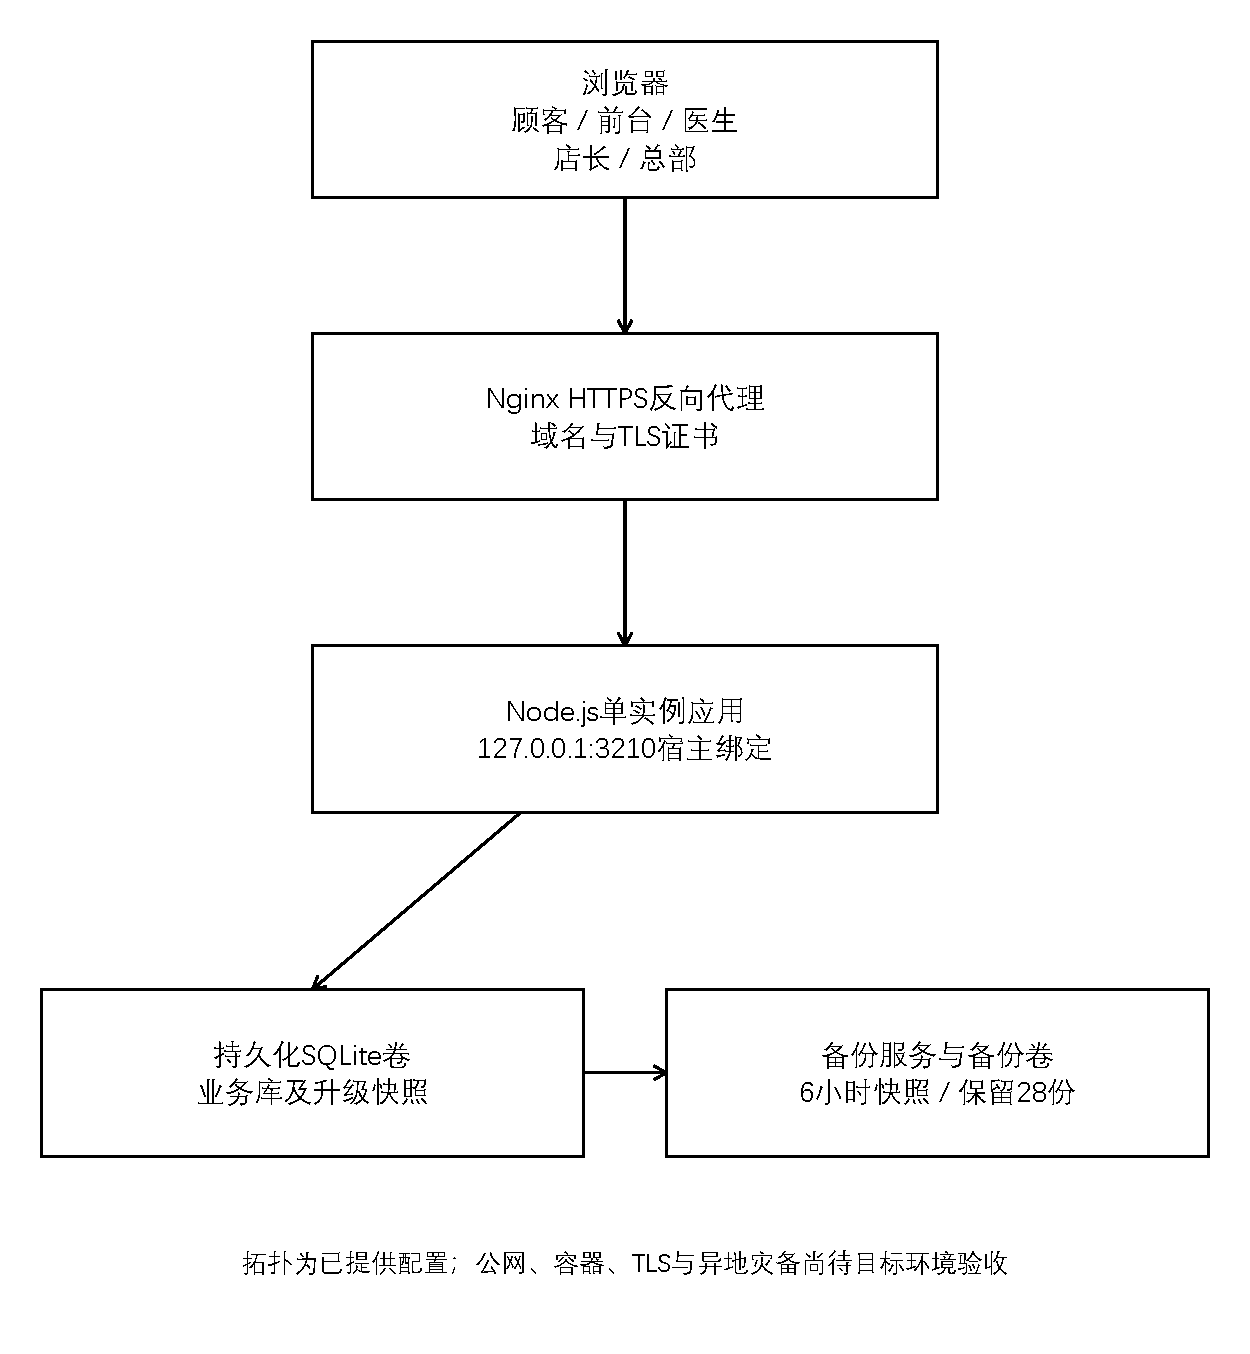
\includegraphics[width=\textwidth]{figures/deployment.pdf}
\caption{单实例部署与备份拓扑}\label{deployment}\end{figure}
独立应用根目录为andrew-system，不依赖课程目录中的旧Clearbrook项目。Dockerfile固定Node.\allowbreak{}js 24.\allowbreak{}15.\allowbreak{}0并以非root用户运行；Compose提供应用与备份服务、持久卷、健康检查、日志轮转及优雅停止。宿主反向代理终止HTTPS，容器应用端口仅绑定宿主回环地址。\par
{\fontsize{10.5pt}{15pt}\selectfont\setlength{\tabcolsep}{0pt}\renewcommand{\arraystretch}{1.08}
\begin{longtable}{@{}p{5.040cm}@{\hspace{0.16cm}}p{10.240cm}@{}}
\caption{部署配置要点}\\
\toprule
\bfseries \Cell{配置} & \bfseries \Cell{正式环境要求}\\\midrule
\endfirsthead
\toprule
\bfseries \Cell{配置} & \bfseries \Cell{正式环境要求}\\\midrule
\endhead
\bottomrule\endlastfoot
\Cell{NODE\_\allowbreak{}ENV} & \Cell{production；启动前检查来源、Cookie及演示设置}\\[3pt]
\Cell{PUBLIC\_\allowbreak{}ORIGIN} & \Cell{准确HTTPS origin，不带路径；多值用逗号分隔}\\[3pt]
\Cell{DENTAL\_\allowbreak{}DB\_\allowbreak{}PATH} & \Cell{持久、可写的SQLite文件位置}\\[3pt]
\Cell{COOKIE\_\allowbreak{}SECURE} & \Cell{1}\\[3pt]
\Cell{DENTAL\_\allowbreak{}SEED\_\allowbreak{}DEMO} & \Cell{0；关闭首次示例填充，不会删除旧演示资料}\\[3pt]
\Cell{DENTAL\_\allowbreak{}PUBLIC\_\allowbreak{}DEMO} & \Cell{仅合成公开演示时显式设置；真实实例不得混入示例账号}\\[3pt]
\Cell{DENTAL\_\allowbreak{}TRUSTED\_\allowbreak{}PROXIES} & \Cell{仅列实际可信代理地址；默认不信任任意转发头}\\[3pt]
\end{longtable}
}
首次正式实例使用独立空库并关闭示例填充，通过accounts.\allowbreak{}mjs初始化店长后录入门诊、医生、治疗与排班，再分配员工。CLI密码通过临时环境变量传入，完成后移除，不进入命令行历史、源码或报告示例。环境文件不由源码自动加载，需进程管理器或显式env-file参数注入。\par
\subsection{备份发布与运行维护}
备份服务默认每6小时使用VACUUM INTO生成一致快照，仅在成功后按规则保留最新28份匹配快照，不删除手工命名备份。数据卷与备份卷分开，但同机卷仍不是异地灾备，需机构另配异地存储和定期恢复演练。升级前另存代码版本和完整快照，停旧服务后迁移，失败回滚并保留证据。\par
GitHub Actions配置包含依赖安装、构建、语法导入检查、自动测试、维护回归、Chromium浏览器回归、合成只读负载和发布清单。发布只包含独立应用源码、构建资源及文档，不上传数据库、快照、环境秘密、依赖目录或测试产物。当前尚未推送GitHub及运行远端Actions，本机也没有Docker引擎，不能把配置文件存在写成容器和公网已验收。\par
\Needspace{9\baselineskip}
\section{测试验证与需求追溯}
\Needspace{7\baselineskip}
\subsection{已有本地验证记录}
{\fontsize{10.5pt}{15pt}\selectfont\setlength{\tabcolsep}{0pt}\renewcommand{\arraystretch}{1.08}
\begin{longtable}{@{}p{2.840cm}@{\hspace{0.16cm}}p{6.340cm}@{\hspace{0.16cm}}p{5.940cm}@{}}
\caption{已记录测试结果及边界}\\
\toprule
\bfseries \Cell{检查} & \bfseries \Cell{2026年10月15日记录} & \bfseries \Cell{能证明与不能证明}\\\midrule
\endfirsthead
\toprule
\bfseries \Cell{检查} & \bfseries \Cell{2026年10月15日记录} & \bfseries \Cell{能证明与不能证明}\\\midrule
\endhead
\bottomrule\endlastfoot
\Cell{自动测试} & \Cell{npm test，48项计数通过、0失败（含父测试计数）} & \Cell{覆盖业务、HTTP、迁移和运维；不穷举临床场景}\\[3pt]
\Cell{浏览器回归} & \Cell{Edge 9项通过} & \Cell{四门户、错身份、局部更新、移动宽度、收款退款冲销和附记；不代表全站可用性试点}\\[3pt]
\Cell{维护检查} & \Cell{16组通过，38表检查} & \Cell{备份、恢复、旧库升级等本地路径；不代表异地灾难恢复}\\[3pt]
\Cell{合成只读负载} & \Cell{1000患者、1000预约，100请求，并发10；总188ms，p50 17ms，p95 29ms} & \Cell{仅该机器和合成读取；不是生产并发承诺}\\[3pt]
\Cell{默认实例升级} & \Cell{完整备份后升级；主要业务数量一致；quick\_\allowbreak{}check=ok，外键错误0} & \Cell{证明该快照升级路径；不代表任意旧库都无需数据清理}\\[3pt]
\end{longtable}
}
本次2026年10月18日文档编制重新核对了源码、DDL及内存PRAGMA，确认38张表、296个字段和58组物理外键；上表沿用10月15日验收记录，日期保留，不将旧结果称为本轮重新执行的性能或浏览器测试。设计文档和ER图不接触真实患者数据。\par
\subsection{需求到实现及测试追溯}
追溯从愿景中的跨店核对开始，经业务责任连接到用例，再落实规则、实体、命令和测试。查询用例对应工作区接口，写入用例对应命令。现有测试未单独覆盖的真实岗位或外部接口场景保留为缺口，避免用一个总通过数替代逐项判断。\par
{\fontsize{10.5pt}{15pt}\selectfont\setlength{\tabcolsep}{0pt}\renewcommand{\arraystretch}{1.08}
\begin{longtable}{@{}p{2.440cm}@{\hspace{0.16cm}}p{12.840cm}@{}}
\toprule
\bfseries \Cell{追溯项} & \bfseries \Cell{内容}\\\midrule
\endfirsthead
\toprule
\bfseries \Cell{追溯项} & \bfseries \Cell{内容}\\\midrule
\endhead
\bottomrule\endlastfoot
\Cell{用例} & \Cell{UC-01 顾客在预约前补全本人身份、联系及过敏声明，使接诊人员获得可核对的资料。}\\[3pt]
\Cell{命令或查询} & \Cell{patient.\allowbreak{}save}\\[3pt]
\Cell{实体与规则} & \Cell{patients；patient\_\allowbreak{}allergies；BR-01；BR-02；BR-03；BR-04}\\[3pt]
\Cell{已有覆盖} & \Cell{test/\allowbreak{}system.\allowbreak{}test.\allowbreak{}js：注册、多项过敏与旧版本保护。}\\[3pt]
\Cell{剩余缺口} & \Cell{本人资料完整浏览器编辑未单独覆盖。}\\[3pt]
\end{longtable}
}
{\fontsize{10.5pt}{15pt}\selectfont\setlength{\tabcolsep}{0pt}\renewcommand{\arraystretch}{1.08}
\begin{longtable}{@{}p{2.440cm}@{\hspace{0.16cm}}p{12.840cm}@{}}
\toprule
\bfseries \Cell{追溯项} & \bfseries \Cell{内容}\\\midrule
\endfirsthead
\toprule
\bfseries \Cell{追溯项} & \bfseries \Cell{内容}\\\midrule
\endhead
\bottomrule\endlastfoot
\Cell{用例} & \Cell{UC-02 为本人或已授权患者选择可用牙医时段，形成可追踪且无时间冲突的有效预约。}\\[3pt]
\Cell{命令或查询} & \Cell{appointment.\allowbreak{}book}\\[3pt]
\Cell{实体与规则} & \Cell{patients；schedules；appointments；dentist\_\allowbreak{}qualifications；qualifications；BR-01；BR-02；BR-04；BR-06；BR-07；BR-30}\\[3pt]
\Cell{已有覆盖} & \Cell{test/\allowbreak{}system.\allowbreak{}test.\allowbreak{}js：竞争预约原子性、未知过敏声明及跨门诊档案检索。}\\[3pt]
\Cell{剩余缺口} & \Cell{所有筛选组合和并发压力下预约未单独覆盖。}\\[3pt]
\end{longtable}
}
{\fontsize{10.5pt}{15pt}\selectfont\setlength{\tabcolsep}{0pt}\renewcommand{\arraystretch}{1.08}
\begin{longtable}{@{}p{2.440cm}@{\hspace{0.16cm}}p{12.840cm}@{}}
\toprule
\bfseries \Cell{追溯项} & \bfseries \Cell{内容}\\\midrule
\endfirsthead
\toprule
\bfseries \Cell{追溯项} & \bfseries \Cell{内容}\\\midrule
\endhead
\bottomrule\endlastfoot
\Cell{用例} & \Cell{UC-03 按业务规则取消有效预约，或将同一就诊需求改到其他可用时段。}\\[3pt]
\Cell{命令或查询} & \Cell{appointment.\allowbreak{}cancel；appointment.\allowbreak{}reschedule}\\[3pt]
\Cell{实体与规则} & \Cell{appointments；schedules；settings；audit；BR-01；BR-02；BR-03；BR-06；BR-07；BR-08；BR-30}\\[3pt]
\Cell{已有覆盖} & \Cell{test/\allowbreak{}system.\allowbreak{}test.\allowbreak{}js：竞争预约及失败改期恢复原预约。；test/\allowbreak{}calendar.\allowbreak{}test.\allowbreak{}js：取消记录不占位。}\\[3pt]
\Cell{剩余缺口} & \Cell{自助截止小时数各边界的浏览器流程未单独覆盖。}\\[3pt]
\end{longtable}
}
{\fontsize{10.5pt}{15pt}\selectfont\setlength{\tabcolsep}{0pt}\renewcommand{\arraystretch}{1.08}
\begin{longtable}{@{}p{2.440cm}@{\hspace{0.16cm}}p{12.840cm}@{}}
\toprule
\bfseries \Cell{追溯项} & \bfseries \Cell{内容}\\\midrule
\endfirsthead
\toprule
\bfseries \Cell{追溯项} & \bfseries \Cell{内容}\\\midrule
\endhead
\bottomrule\endlastfoot
\Cell{用例} & \Cell{UC-04 顾客查询本人历史就诊、治疗明细、结算及收退款状态，核对费用并按需打印结算单。}\\[3pt]
\Cell{命令或查询} & \Cell{GET /\allowbreak{}api/\allowbreak{}workspace?page=history；GET /\allowbreak{}api/\allowbreak{}workspace?page=settlements}\\[3pt]
\Cell{实体与规则} & \Cell{visits；visit\_\allowbreak{}lines；visit\_\allowbreak{}addenda；settlements；settlement\_\allowbreak{}lines；payments；refunds；invoice\_\allowbreak{}adjustments；BR-01；BR-02；BR-11；BR-12；BR-13；BR-29}\\[3pt]
\Cell{已有覆盖} & \Cell{test/\allowbreak{}system.\allowbreak{}test.\allowbreak{}js：本人范围保护、完整诊疗结算链及重启持久化。}\\[3pt]
\Cell{剩余缺口} & \Cell{结算单浏览器打印及多页历史完整交互未单独覆盖。}\\[3pt]
\end{longtable}
}
{\fontsize{10.5pt}{15pt}\selectfont\setlength{\tabcolsep}{0pt}\renewcommand{\arraystretch}{1.08}
\begin{longtable}{@{}p{2.440cm}@{\hspace{0.16cm}}p{12.840cm}@{}}
\toprule
\bfseries \Cell{追溯项} & \bfseries \Cell{内容}\\\midrule
\endfirsthead
\toprule
\bfseries \Cell{追溯项} & \bfseries \Cell{内容}\\\midrule
\endhead
\bottomrule\endlastfoot
\Cell{用例} & \Cell{UC-05 工作人员检索、核对和维护授权患者资料，跨门诊就诊优先复用既有档案。}\\[3pt]
\Cell{命令或查询} & \Cell{patient.\allowbreak{}lookup；patient.\allowbreak{}save}\\[3pt]
\Cell{实体与规则} & \Cell{patients；patient\_\allowbreak{}allergies；patient\_\allowbreak{}clinic\_\allowbreak{}access；appointments；BR-01；BR-02；BR-03；BR-04；BR-05}\\[3pt]
\Cell{已有覆盖} & \Cell{test/\allowbreak{}system.\allowbreak{}test.\allowbreak{}js：核验跨门诊检索、范围保护和旧版本保护。}\\[3pt]
\Cell{剩余缺口} & \Cell{新增患者完整浏览器编辑未单独覆盖。}\\[3pt]
\end{longtable}
}
{\fontsize{10.5pt}{15pt}\selectfont\setlength{\tabcolsep}{0pt}\renewcommand{\arraystretch}{1.08}
\begin{longtable}{@{}p{2.440cm}@{\hspace{0.16cm}}p{12.840cm}@{}}
\toprule
\bfseries \Cell{追溯项} & \bfseries \Cell{内容}\\\midrule
\endfirsthead
\toprule
\bfseries \Cell{追溯项} & \bfseries \Cell{内容}\\\midrule
\endhead
\bottomrule\endlastfoot
\Cell{用例} & \Cell{UC-06 维护门诊基本资料和牙医未来接诊时段，使预约资源与实际接诊安排保持一致。}\\[3pt]
\Cell{命令或查询} & \Cell{clinic.\allowbreak{}save；schedule.\allowbreak{}save}\\[3pt]
\Cell{实体与规则} & \Cell{clinics；schedules；dentists；qualifications；appointments；quarterReports；BR-01；BR-02；BR-03；BR-06；BR-07；BR-10；BR-27}\\[3pt]
\Cell{已有覆盖} & \Cell{test/\allowbreak{}system.\allowbreak{}test.\allowbreak{}js：跨门诊排班冲突、资格守卫与输入校验。}\\[3pt]
\Cell{剩余缺口} & \Cell{诊所完整编辑和停用界面未单独覆盖。}\\[3pt]
\end{longtable}
}
{\fontsize{10.5pt}{15pt}\selectfont\setlength{\tabcolsep}{0pt}\renewcommand{\arraystretch}{1.08}
\begin{longtable}{@{}p{2.440cm}@{\hspace{0.16cm}}p{12.840cm}@{}}
\toprule
\bfseries \Cell{追溯项} & \bfseries \Cell{内容}\\\midrule
\endfirsthead
\toprule
\bfseries \Cell{追溯项} & \bfseries \Cell{内容}\\\midrule
\endhead
\bottomrule\endlastfoot
\Cell{用例} & \Cell{UC-07 由店长建立牙医档案、维护有效资格及核验资料，形成可参与排班的人员基础。}\\[3pt]
\Cell{命令或查询} & \Cell{dentist.\allowbreak{}save；qualification.\allowbreak{}save}\\[3pt]
\Cell{实体与规则} & \Cell{dentists；qualifications；dentist\_\allowbreak{}qualifications；dentist\_\allowbreak{}qualification\_\allowbreak{}details；BR-01；BR-03；BR-10}\\[3pt]
\Cell{已有覆盖} & \Cell{test/\allowbreak{}system.\allowbreak{}test.\allowbreak{}js：资格守卫及不合法明细检查。}\\[3pt]
\Cell{剩余缺口} & \Cell{资格证书核验字段未逐项测试，完整资源维护界面未单独覆盖。}\\[3pt]
\end{longtable}
}
{\fontsize{10.5pt}{15pt}\selectfont\setlength{\tabcolsep}{0pt}\renewcommand{\arraystretch}{1.08}
\begin{longtable}{@{}p{2.440cm}@{\hspace{0.16cm}}p{12.840cm}@{}}
\toprule
\bfseries \Cell{追溯项} & \bfseries \Cell{内容}\\\midrule
\endfirsthead
\toprule
\bfseries \Cell{追溯项} & \bfseries \Cell{内容}\\\midrule
\endhead
\bottomrule\endlastfoot
\Cell{用例} & \Cell{UC-08 前台在授权门诊确认到诊或爽约，并在误记时按规则更正出席状态。}\\[3pt]
\Cell{命令或查询} & \Cell{appointment.\allowbreak{}status}\\[3pt]
\Cell{实体与规则} & \Cell{appointments；visits；schedules；BR-01；BR-02；BR-03；BR-09}\\[3pt]
\Cell{已有覆盖} & \Cell{test/\allowbreak{}system.\allowbreak{}test.\allowbreak{}js：出席时间守卫及前台到诊—医生诊疗—开单完整链。}\\[3pt]
\Cell{剩余缺口} & \Cell{爽约恢复及重复到诊完整交互未单独覆盖。}\\[3pt]
\end{longtable}
}
{\fontsize{10.5pt}{15pt}\selectfont\setlength{\tabcolsep}{0pt}\renewcommand{\arraystretch}{1.08}
\begin{longtable}{@{}p{2.440cm}@{\hspace{0.16cm}}p{12.840cm}@{}}
\toprule
\bfseries \Cell{追溯项} & \bfseries \Cell{内容}\\\midrule
\endfirsthead
\toprule
\bfseries \Cell{追溯项} & \bfseries \Cell{内容}\\\midrule
\endhead
\bottomrule\endlastfoot
\Cell{用例} & \Cell{UC-09 接诊医生记录治疗项目和备注，核对后完成就诊，使后续开单具有稳定依据。}\\[3pt]
\Cell{命令或查询} & \Cell{visit.\allowbreak{}save；visit.\allowbreak{}complete}\\[3pt]
\Cell{实体与规则} & \Cell{visits；visit\_\allowbreak{}lines；treatments；patients；patient\_\allowbreak{}allergies；BR-01；BR-02；BR-03；BR-11}\\[3pt]
\Cell{已有覆盖} & \Cell{test/\allowbreak{}system.\allowbreak{}test.\allowbreak{}js：完整接诊链、目录调价不改历史、完成后锁定。；test/\allowbreak{}business.\allowbreak{}test.\allowbreak{}js：附记边界。}\\[3pt]
\Cell{剩余缺口} & \Cell{治疗表单各数量边界的浏览器流程未单独覆盖。}\\[3pt]
\end{longtable}
}
{\fontsize{10.5pt}{15pt}\selectfont\setlength{\tabcolsep}{0pt}\renewcommand{\arraystretch}{1.08}
\begin{longtable}{@{}p{2.440cm}@{\hspace{0.16cm}}p{12.840cm}@{}}
\toprule
\bfseries \Cell{追溯项} & \bfseries \Cell{内容}\\\midrule
\endfirsthead
\toprule
\bfseries \Cell{追溯项} & \bfseries \Cell{内容}\\\midrule
\endhead
\bottomrule\endlastfoot
\Cell{用例} & \Cell{UC-10 前台将已完成就诊的治疗快照生成唯一结算单，向患者提供可核对的费用明细。}\\[3pt]
\Cell{命令或查询} & \Cell{settlement.\allowbreak{}create}\\[3pt]
\Cell{实体与规则} & \Cell{settlements；settlement\_\allowbreak{}lines；visits；visit\_\allowbreak{}lines；quarterReports；BR-01；BR-02；BR-11；BR-12；BR-27}\\[3pt]
\Cell{已有覆盖} & \Cell{test/\allowbreak{}system.\allowbreak{}test.\allowbreak{}js：完成诊疗后开单、重复返回原单、价格快照及顾客详情一致。}\\[3pt]
\Cell{剩余缺口} & \Cell{浏览器打印及异常单据金额边界未逐项单独覆盖。}\\[3pt]
\end{longtable}
}
{\fontsize{10.5pt}{15pt}\selectfont\setlength{\tabcolsep}{0pt}\renewcommand{\arraystretch}{1.08}
\begin{longtable}{@{}p{2.440cm}@{\hspace{0.16cm}}p{12.840cm}@{}}
\toprule
\bfseries \Cell{追溯项} & \bfseries \Cell{内容}\\\midrule
\endfirsthead
\toprule
\bfseries \Cell{追溯项} & \bfseries \Cell{内容}\\\midrule
\endhead
\bottomrule\endlastfoot
\Cell{用例} & \Cell{UC-11 店长按指定季度核对预约履约、成本与已有季度报告，识别需要进一步处理的差异。}\\[3pt]
\Cell{命令或查询} & \Cell{GET /\allowbreak{}api/\allowbreak{}workspace?page=performance\&quarter=YYYY-Qn}\\[3pt]
\Cell{实体与规则} & \Cell{appointments；costs；quarterReports；quarter\_\allowbreak{}report\_\allowbreak{}rows；BR-01；BR-25；BR-28；BR-29}\\[3pt]
\Cell{已有覆盖} & \Cell{test/\allowbreak{}operations.\allowbreak{}test.\allowbreak{}js：季度指标窗口与分页。；test/\allowbreak{}system.\allowbreak{}test.\allowbreak{}js：成本和报告一致性。}\\[3pt]
\Cell{剩余缺口} & \Cell{季度业绩完整浏览器核对未单独覆盖。}\\[3pt]
\end{longtable}
}
{\fontsize{10.5pt}{15pt}\selectfont\setlength{\tabcolsep}{0pt}\renewcommand{\arraystretch}{1.08}
\begin{longtable}{@{}p{2.440cm}@{\hspace{0.16cm}}p{12.840cm}@{}}
\toprule
\bfseries \Cell{追溯项} & \bfseries \Cell{内容}\\\midrule
\endfirsthead
\toprule
\bfseries \Cell{追溯项} & \bfseries \Cell{内容}\\\midrule
\endhead
\bottomrule\endlastfoot
\Cell{用例} & \Cell{UC-12 店长在成本完整且已审核的基础上生成全连锁季度报告，并确认净利润与激励基金。}\\[3pt]
\Cell{命令或查询} & \Cell{quarter.\allowbreak{}compute；quarter.\allowbreak{}approve}\\[3pt]
\Cell{实体与规则} & \Cell{costs；settlements；invoice\_\allowbreak{}adjustments；schedules；quarterReports；quarter\_\allowbreak{}report\_\allowbreak{}rows；quarter\_\allowbreak{}report\_\allowbreak{}settlements；quarter\_\allowbreak{}report\_\allowbreak{}history；BR-01；BR-03；BR-25；BR-26；BR-27}\\[3pt]
\Cell{已有覆盖} & \Cell{test/\allowbreak{}system.\allowbreak{}test.\allowbreak{}js：成本完整、基金批准、修订使来源失效。；test/\allowbreak{}business.\allowbreak{}test.\allowbreak{}js：冲销影响季度收入。}\\[3pt]
\Cell{剩余缺口} & \Cell{负利润等所有边界组合及完整报告批准界面未逐项覆盖。}\\[3pt]
\end{longtable}
}
{\fontsize{10.5pt}{15pt}\selectfont\setlength{\tabcolsep}{0pt}\renewcommand{\arraystretch}{1.08}
\begin{longtable}{@{}p{2.440cm}@{\hspace{0.16cm}}p{12.840cm}@{}}
\toprule
\bfseries \Cell{追溯项} & \bfseries \Cell{内容}\\\midrule
\endfirsthead
\toprule
\bfseries \Cell{追溯项} & \bfseries \Cell{内容}\\\midrule
\endhead
\bottomrule\endlastfoot
\Cell{用例} & \Cell{UC-13 前台在人工确认资金到账后登记结算单收款，更新净实收与欠款。}\\[3pt]
\Cell{命令或查询} & \Cell{payment.\allowbreak{}record}\\[3pt]
\Cell{实体与规则} & \Cell{settlements；payments；refunds；invoice\_\allowbreak{}adjustments；idempotency\_\allowbreak{}requests；BR-01；BR-02；BR-13；BR-14；BR-30}\\[3pt]
\Cell{已有覆盖} & \Cell{test/\allowbreak{}business.\allowbreak{}test.\allowbreak{}js：金额、授权、幂等和余额。；test/\allowbreak{}http-engineering.\allowbreak{}test.\allowbreak{}js：HTTP重放。；test/\allowbreak{}browser/\allowbreak{}workspaces.\allowbreak{}spec.\allowbreak{}js：账务链。}\\[3pt]
\Cell{剩余缺口} & \Cell{真实收款渠道到账未接入，测试不证明实际资金到账。}\\[3pt]
\end{longtable}
}
{\fontsize{10.5pt}{15pt}\selectfont\setlength{\tabcolsep}{0pt}\renewcommand{\arraystretch}{1.08}
\begin{longtable}{@{}p{2.440cm}@{\hspace{0.16cm}}p{12.840cm}@{}}
\toprule
\bfseries \Cell{追溯项} & \bfseries \Cell{内容}\\\midrule
\endfirsthead
\toprule
\bfseries \Cell{追溯项} & \bfseries \Cell{内容}\\\midrule
\endhead
\bottomrule\endlastfoot
\Cell{用例} & \Cell{UC-14 店长在线下执行并核对实际退款后，针对原收款追加退款流水。}\\[3pt]
\Cell{命令或查询} & \Cell{payment.\allowbreak{}refund}\\[3pt]
\Cell{实体与规则} & \Cell{payments；refunds；settlements；idempotency\_\allowbreak{}requests；BR-01；BR-13；BR-14；BR-30}\\[3pt]
\Cell{已有覆盖} & \Cell{test/\allowbreak{}business.\allowbreak{}test.\allowbreak{}js：退款上限与退款后冲销。；test/\allowbreak{}browser/\allowbreak{}workspaces.\allowbreak{}spec.\allowbreak{}js：原款退款界面。}\\[3pt]
\Cell{剩余缺口} & \Cell{真实退款渠道未接入，测试不证明实际资金退回。}\\[3pt]
\end{longtable}
}
{\fontsize{10.5pt}{15pt}\selectfont\setlength{\tabcolsep}{0pt}\renewcommand{\arraystretch}{1.08}
\begin{longtable}{@{}p{2.440cm}@{\hspace{0.16cm}}p{12.840cm}@{}}
\toprule
\bfseries \Cell{追溯项} & \bfseries \Cell{内容}\\\midrule
\endfirsthead
\toprule
\bfseries \Cell{追溯项} & \bfseries \Cell{内容}\\\midrule
\endhead
\bottomrule\endlastfoot
\Cell{用例} & \Cell{UC-15 店长在款项已完整退回后，通过独立调整记录冲销错误结算单并保留原单。}\\[3pt]
\Cell{命令或查询} & \Cell{settlement.\allowbreak{}void}\\[3pt]
\Cell{实体与规则} & \Cell{settlements；invoice\_\allowbreak{}adjustments；payments；refunds；quarterReports；BR-01；BR-03；BR-15；BR-27}\\[3pt]
\Cell{已有覆盖} & \Cell{test/\allowbreak{}business.\allowbreak{}test.\allowbreak{}js：先完整退款再冲销、原单不变及季度调整。；test/\allowbreak{}browser/\allowbreak{}workspaces.\allowbreak{}spec.\allowbreak{}js：账务链。}\\[3pt]
\Cell{剩余缺口} & \Cell{零金额冲销和重复冲销的独立界面流程未单独覆盖。}\\[3pt]
\end{longtable}
}
{\fontsize{10.5pt}{15pt}\selectfont\setlength{\tabcolsep}{0pt}\renewcommand{\arraystretch}{1.08}
\begin{longtable}{@{}p{2.440cm}@{\hspace{0.16cm}}p{12.840cm}@{}}
\toprule
\bfseries \Cell{追溯项} & \bfseries \Cell{内容}\\\midrule
\endfirsthead
\toprule
\bfseries \Cell{追溯项} & \bfseries \Cell{内容}\\\midrule
\endhead
\bottomrule\endlastfoot
\Cell{用例} & \Cell{UC-16 前台或店长按门诊和北京时间营业日核对渠道净额，并保留差额和修订原因。}\\[3pt]
\Cell{命令或查询} & \Cell{reconciliation.\allowbreak{}preview；reconciliation.\allowbreak{}record}\\[3pt]
\Cell{实体与规则} & \Cell{reconciliations；payments；refunds；settlements；BR-01；BR-02；BR-13；BR-14；BR-16}\\[3pt]
\Cell{已有覆盖} & \Cell{test/\allowbreak{}business.\allowbreak{}test.\allowbreak{}js：北京时间日结、差额、不可覆盖修订和来源失效。}\\[3pt]
\Cell{剩余缺口} & \Cell{完整日结界面流程及所有渠道差额组合未单独覆盖。}\\[3pt]
\end{longtable}
}
{\fontsize{10.5pt}{15pt}\selectfont\setlength{\tabcolsep}{0pt}\renewcommand{\arraystretch}{1.08}
\begin{longtable}{@{}p{2.440cm}@{\hspace{0.16cm}}p{12.840cm}@{}}
\toprule
\bfseries \Cell{追溯项} & \bfseries \Cell{内容}\\\midrule
\endfirsthead
\toprule
\bfseries \Cell{追溯项} & \bfseries \Cell{内容}\\\midrule
\endhead
\bottomrule\endlastfoot
\Cell{用例} & \Cell{UC-17 接诊医生对已完成记录补充更正说明，保留原文、作者、时间和所依据版本。}\\[3pt]
\Cell{命令或查询} & \Cell{visit.\allowbreak{}addendum}\\[3pt]
\Cell{实体与规则} & \Cell{visits；visit\_\allowbreak{}addenda；users；BR-01；BR-02；BR-03；BR-17}\\[3pt]
\Cell{已有覆盖} & \Cell{test/\allowbreak{}business.\allowbreak{}test.\allowbreak{}js：接诊医生及店长权限、不可覆盖附记。；test/\allowbreak{}browser/\allowbreak{}workspaces.\allowbreak{}spec.\allowbreak{}js：追加并读取附记。}\\[3pt]
\Cell{剩余缺口} & \Cell{附记最大长度等全部边界未逐项单独覆盖。}\\[3pt]
\end{longtable}
}
{\fontsize{10.5pt}{15pt}\selectfont\setlength{\tabcolsep}{0pt}\renewcommand{\arraystretch}{1.08}
\begin{longtable}{@{}p{2.440cm}@{\hspace{0.16cm}}p{12.840cm}@{}}
\toprule
\bfseries \Cell{追溯项} & \bfseries \Cell{内容}\\\midrule
\endfirsthead
\toprule
\bfseries \Cell{追溯项} & \bfseries \Cell{内容}\\\midrule
\endhead
\bottomrule\endlastfoot
\Cell{用例} & \Cell{UC-18 店长完成身份核验后归并两份同一患者档案，保留来源别名并迁移业务关联。}\\[3pt]
\Cell{命令或查询} & \Cell{patient.\allowbreak{}merge}\\[3pt]
\Cell{实体与规则} & \Cell{patients；patient\_\allowbreak{}allergies；patient\_\allowbreak{}clinic\_\allowbreak{}access；appointments；visits；settlements；patient\_\allowbreak{}aliases；users；sessions；BR-01；BR-03；BR-18；BR-19}\\[3pt]
\Cell{已有覆盖} & \Cell{test/\allowbreak{}business.\allowbreak{}test.\allowbreak{}js：迁移引用、保留别名、撤销会话、身份冲突及双有效账号拒绝。}\\[3pt]
\Cell{剩余缺口} & \Cell{多来源连续归并及完整归并界面未单独覆盖。}\\[3pt]
\end{longtable}
}
{\fontsize{10.5pt}{15pt}\selectfont\setlength{\tabcolsep}{0pt}\renewcommand{\arraystretch}{1.08}
\begin{longtable}{@{}p{2.440cm}@{\hspace{0.16cm}}p{12.840cm}@{}}
\toprule
\bfseries \Cell{追溯项} & \bfseries \Cell{内容}\\\midrule
\endfirsthead
\toprule
\bfseries \Cell{追溯项} & \bfseries \Cell{内容}\\\midrule
\endhead
\bottomrule\endlastfoot
\Cell{用例} & \Cell{UC-19 店长为已有患者档案建立顾客登录账号，避免自助注册重复建档或公开认领。}\\[3pt]
\Cell{命令或查询} & \Cell{account.\allowbreak{}bindCustomer}\\[3pt]
\Cell{实体与规则} & \Cell{patients；users；audit；BR-01；BR-03；BR-20；BR-22；BR-24}\\[3pt]
\Cell{已有覆盖} & \Cell{test/\allowbreak{}business.\allowbreak{}test.\allowbreak{}js：机构核验绑定与防重复认领。；test/\allowbreak{}http-engineering.\allowbreak{}test.\allowbreak{}js：已有电话注册不重复建档。}\\[3pt]
\Cell{剩余缺口} & \Cell{机构线下身份核验不属于自动测试覆盖；完整绑定界面未单独覆盖。}\\[3pt]
\end{longtable}
}
{\fontsize{10.5pt}{15pt}\selectfont\setlength{\tabcolsep}{0pt}\renewcommand{\arraystretch}{1.08}
\begin{longtable}{@{}p{2.440cm}@{\hspace{0.16cm}}p{12.840cm}@{}}
\toprule
\bfseries \Cell{追溯项} & \bfseries \Cell{内容}\\\midrule
\endfirsthead
\toprule
\bfseries \Cell{追溯项} & \bfseries \Cell{内容}\\\midrule
\endhead
\bottomrule\endlastfoot
\Cell{用例} & \Cell{UC-20 店长创建员工账号、调整岗位归属并办理停用或离职，使访问范围随人员状态变化。}\\[3pt]
\Cell{命令或查询} & \Cell{account.\allowbreak{}create；account.\allowbreak{}assign；account.\allowbreak{}status}\\[3pt]
\Cell{实体与规则} & \Cell{users；clinics；dentists；sessions；password\_\allowbreak{}reset\_\allowbreak{}tokens；BR-01；BR-03；BR-21；BR-22；BR-24}\\[3pt]
\Cell{已有覆盖} & \Cell{test/\allowbreak{}business.\allowbreak{}test.\allowbreak{}js：范围、版本、撤销及自停保护。；test/\allowbreak{}http-engineering.\allowbreak{}test.\allowbreak{}js：停用后Cookie和登录立即失效。}\\[3pt]
\Cell{剩余缺口} & \Cell{离职后的全部状态转换和完整人员管理界面未逐项覆盖。}\\[3pt]
\end{longtable}
}
{\fontsize{10.5pt}{15pt}\selectfont\setlength{\tabcolsep}{0pt}\renewcommand{\arraystretch}{1.08}
\begin{longtable}{@{}p{2.440cm}@{\hspace{0.16cm}}p{12.840cm}@{}}
\toprule
\bfseries \Cell{追溯项} & \bfseries \Cell{内容}\\\midrule
\endfirsthead
\toprule
\bfseries \Cell{追溯项} & \bfseries \Cell{内容}\\\midrule
\endhead
\bottomrule\endlastfoot
\Cell{用例} & \Cell{UC-21 已登录用户验证原密码后更换本人密码，并强制以新密码重新登录。}\\[3pt]
\Cell{命令或查询} & \Cell{password.\allowbreak{}change}\\[3pt]
\Cell{实体与规则} & \Cell{users；sessions；password\_\allowbreak{}reset\_\allowbreak{}tokens；BR-01；BR-22；BR-24}\\[3pt]
\Cell{已有覆盖} & \Cell{test/\allowbreak{}business.\allowbreak{}test.\allowbreak{}js：原密码验证、改密撤销和审计脱敏。}\\[3pt]
\Cell{剩余缺口} & \Cell{改密完整浏览器流程未单独覆盖。}\\[3pt]
\end{longtable}
}
{\fontsize{10.5pt}{15pt}\selectfont\setlength{\tabcolsep}{0pt}\renewcommand{\arraystretch}{1.08}
\begin{longtable}{@{}p{2.440cm}@{\hspace{0.16cm}}p{12.840cm}@{}}
\toprule
\bfseries \Cell{追溯项} & \bfseries \Cell{内容}\\\midrule
\endfirsthead
\toprule
\bfseries \Cell{追溯项} & \bfseries \Cell{内容}\\\midrule
\endhead
\bottomrule\endlastfoot
\Cell{用例} & \Cell{UC-22 忘记密码的用户经机构核验获得一次性恢复码，设置新密码后重新登录。}\\[3pt]
\Cell{命令或查询} & \Cell{POST /\allowbreak{}api/\allowbreak{}password-recovery/\allowbreak{}request；account.\allowbreak{}issueRecovery；POST /\allowbreak{}api/\allowbreak{}password-recovery/\allowbreak{}consume}\\[3pt]
\Cell{实体与规则} & \Cell{account\_\allowbreak{}recovery\_\allowbreak{}requests；password\_\allowbreak{}reset\_\allowbreak{}tokens；users；sessions；audit；BR-01；BR-22；BR-23；BR-24}\\[3pt]
\Cell{已有覆盖} & \Cell{test/\allowbreak{}business.\allowbreak{}test.\allowbreak{}js：单次恢复和会话撤销。；test/\allowbreak{}http-engineering.\allowbreak{}test.\allowbreak{}js：统一响应、秘密不缓存及不可重复消费。}\\[3pt]
\Cell{剩余缺口} & \Cell{机构当面交付与线下身份核验不属于自动测试覆盖。}\\[3pt]
\end{longtable}
}
{\fontsize{10.5pt}{15pt}\selectfont\setlength{\tabcolsep}{0pt}\renewcommand{\arraystretch}{1.08}
\begin{longtable}{@{}p{2.440cm}@{\hspace{0.16cm}}p{12.840cm}@{}}
\toprule
\bfseries \Cell{追溯项} & \bfseries \Cell{内容}\\\midrule
\endfirsthead
\toprule
\bfseries \Cell{追溯项} & \bfseries \Cell{内容}\\\midrule
\endhead
\bottomrule\endlastfoot
\Cell{用例} & \Cell{UC-23 店长按季度、门诊和牙医记录有依据的用品及运营成本，审核后供基金核算引用。}\\[3pt]
\Cell{命令或查询} & \Cell{cost.\allowbreak{}save；cost.\allowbreak{}review}\\[3pt]
\Cell{实体与规则} & \Cell{costs；cost\_\allowbreak{}review\_\allowbreak{}history；quarterReports；quarter\_\allowbreak{}report\_\allowbreak{}history；BR-01；BR-03；BR-25；BR-27}\\[3pt]
\Cell{已有覆盖} & \Cell{test/\allowbreak{}system.\allowbreak{}test.\allowbreak{}js：成本修订重置审核并使旧报告失效、缺成本拒绝核算。}\\[3pt]
\Cell{剩余缺口} & \Cell{成本独立浏览器操作和双人复核未覆盖；当前未实现双人复核。}\\[3pt]
\end{longtable}
}
{\fontsize{10.5pt}{15pt}\selectfont\setlength{\tabcolsep}{0pt}\renewcommand{\arraystretch}{1.08}
\begin{longtable}{@{}p{2.440cm}@{\hspace{0.16cm}}p{12.840cm}@{}}
\toprule
\bfseries \Cell{追溯项} & \bfseries \Cell{内容}\\\midrule
\endfirsthead
\toprule
\bfseries \Cell{追溯项} & \bfseries \Cell{内容}\\\midrule
\endhead
\bottomrule\endlastfoot
\Cell{用例} & \Cell{UC-24 店长导出全门诊业务 JSON 留存，用于人工检查和数据交接。}\\[3pt]
\Cell{命令或查询} & \Cell{GET /\allowbreak{}api/\allowbreak{}backup}\\[3pt]
\Cell{实体与规则} & \Cell{clinics；dentists；qualifications；dentist\_\allowbreak{}qualifications；dentist\_\allowbreak{}qualification\_\allowbreak{}details；treatments；patients；patient\_\allowbreak{}allergies；patient\_\allowbreak{}clinic\_\allowbreak{}access；schedules；appointments；visits；visit\_\allowbreak{}lines；settlements；settlement\_\allowbreak{}lines；costs；cost\_\allowbreak{}review\_\allowbreak{}history；quarterReports；quarter\_\allowbreak{}report\_\allowbreak{}clinics；quarter\_\allowbreak{}report\_\allowbreak{}rows；quarter\_\allowbreak{}report\_\allowbreak{}settlements；quarter\_\allowbreak{}report\_\allowbreak{}history；settings；payments；refunds；invoice\_\allowbreak{}adjustments；reconciliations；visit\_\allowbreak{}addenda；patient\_\allowbreak{}aliases；audit；BR-01；BR-31}\\[3pt]
\Cell{已有覆盖} & \Cell{test/\allowbreak{}system.\allowbreak{}test.\allowbreak{}js：前台导出被拒、店长导出成功及凭证排除。}\\[3pt]
\Cell{剩余缺口} & \Cell{浏览器附件保存与导出后下游交接未单独覆盖。}\\[3pt]
\end{longtable}
}
\Needspace{7\baselineskip}
\subsection{课程工件覆盖与待验收事项}
{\fontsize{10.5pt}{15pt}\selectfont\setlength{\tabcolsep}{0pt}\renewcommand{\arraystretch}{1.08}
\begin{longtable}{@{}p{3.240cm}@{\hspace{0.16cm}}p{3.240cm}@{\hspace{0.16cm}}p{8.640cm}@{}}
\caption{课程工件对应表}\\
\toprule
\bfseries \Cell{课程工件} & \bfseries \Cell{课件物理页} & \bfseries \Cell{本报告对应内容}\\\midrule
\endfirsthead
\toprule
\bfseries \Cell{课程工件} & \bfseries \Cell{课件物理页} & \bfseries \Cell{本报告对应内容}\\\midrule
\endhead
\bottomrule\endlastfoot
\Cell{愿景} & \Cell{32、59—81} & \Cell{愿景指标、度量办法及未采集的基线}\\[3pt]
\Cell{业务模型} & \Cell{85—127} & \Cell{业务用例、三类现状及三类改进业务序列}\\[3pt]
\Cell{系统需求} & \Cell{138—205} & \Cell{四角色系统用例、24份完整规约、质量与规则}\\[3pt]
\Cell{面向对象分析} & \Cell{285—357} & \Cell{分析类图、预约分析序列、对象状态与不变式}\\[3pt]
\Cell{四架构型练习} & \Cell{385—387} & \Cell{架构型映射、牙医资源状态机及创建时段交互示例}\\[3pt]
\Cell{数据库映射} & \Cell{397—403} & \Cell{概念及物理ER、范式、38表字典、键和索引}\\[3pt]
\Cell{设计实现} & \Cell{388—441} & \Cell{分层、服务职责、表示层、事务与部署}\\[3pt]
\end{longtable}
}
正式试点前还需完成：真实门诊身份和健康核验制度、岗位任务可用性测试、真实数据清理与迁移抽查、目标主机容量、容器及HTTPS联调、异地备份恢复演练，以及完整临床记录和外部支付/\allowbreak{}票据接口的范围确认。没有实际上线记录时，不承诺可用率、临床安全性或资金实时结算能力。\par
\section{结论}
本设计将跨门诊统一患者档案作为协作主线，明确四角色边界，使用独立预约、就诊、结算和资金记录保持业务语义。课程所要求的业务、需求、分析与设计工件可以通过编号、关系和责任映射相互核对，数据库ER和字段字典也与当前实现保持一致。\par
当前系统完成了本地可运行的就诊与运营协作，实现了关键一致性和维护机制。后续工作的重点是机构试点、完整临床范围及目标环境验收，再依据真实负载演进基础设施，而不是将课程原型直接描述为成熟医院生产系统。\par
\section*{参考文献}
\phantomsection\addcontentsline{toc}{section}{参考文献}
\noindent [1] 系统分析与设计 精简2026-9[Z]. 用户提供课程课件，2026.9更新，共441页；方法引用物理页19—23、85—127、154、285—357、385—403、408—441。\par
\noindent [2] 安德鲁牙科连锁店 数据建模 Andrew’s Dental Chain[Z]. 课程案例，3页；沿用既有案例提取及业务建模资料。\par
\noindent [3] 中南大学湘雅口腔医院. 就诊须知[EB/OL]. \url{https://xykqyy.csu.edu.cn/ylfw/jzxz.htm}，访问2026-10-18。\par
\noindent [4] 中南大学湘雅口腔医院. 就诊流程[EB/OL]. \url{https://xykqyy.csu.edu.cn/ylfw/jzlc.htm}，海报整理2026-10-08，页面复核2026-10-18。\par
\noindent [5] 中南大学湘雅口腔医院. 2026年10月门诊排班公示[EB/OL]. 2026-09-30. \url{https://xykqyy.csu.edu.cn/info/1153/12089.htm}，访问2026-10-18。\par
\noindent [6] 中南大学湘雅口腔医院. 牙周科卓越护理报道[EB/OL]. 2024-08-23. \url{https://xykqyy.csu.edu.cn/info/1105/10351.htm}，访问2026-10-18；口腔修复科、种植中心报道，2024-08-27，\url{https://xykqyy.csu.edu.cn/info/1105/10355.htm}，历史整理2026-10-08。\par
\noindent [7] 中南大学湘雅口腔医院. 关于执行湖南省医疗服务价格项目目录2024年版的公告[EB/OL]. 2024-04-30. \url{https://xykqyy.csu.edu.cn/info/1153/10104.htm}，访问2026-10-18。\par
\noindent [8] 中南大学湘雅口腔医院. 信息化建设项目采购意向公告[EB/OL]. 2021-06-11. \url{https://xykqyy.csu.edu.cn/info/1259/11431.htm}，访问2026-10-18。\par
\noindent [9] 中南大学湘雅口腔医院. 医疗收费电子票据管理系统项目中标公示[EB/OL]. 2024-04-30. \url{https://xykqyy.csu.edu.cn/info/1259/11321.htm}，访问2026-10-18。\par
\noindent [10] Node.js. SQLite API[EB/OL]. \url{https://nodejs.org/api/sqlite.html}；SQLite. Foreign Key Support[EB/OL]. \url{https://www.sqlite.org/foreignkeys.html}，访问2026-10-18。\par
\noindent [11] 安德鲁牙科就诊与运营系统3.0源码及本地验收记录[CP/OL]. andrew-system/server/schema.sql、server/migrations/extensions.sql、server/services、API-CONTRACT.md、REFACTOR-ACCEPTANCE.md；源码核对2026-10-18，测试记录2026-10-15。\par
\appendix
\section{完整数据库字段字典}
本附录由当前两份DDL在临时内存SQLite中执行后提取，覆盖38表和296字段。N表示显式或整数主键隐含不可空，Y表示当前DDL允许空；PK*表示业务主键必填但普通TEXT主键未显式NOT NULL。联合主键及外键顺序按DDL保留。默认“—”表示没有声明默认值，不等于默认空字符串。\par
\subsection{metadata 系统元数据}
记录初始化版本等键值元数据。 来源：server/\allowbreak{}schema.\allowbreak{}sql。\par
{\fontsize{10.5pt}{15pt}\selectfont\setlength{\tabcolsep}{0pt}\renewcommand{\arraystretch}{1.08}
\begin{longtable}{@{}p{4.040cm}@{\hspace{0.16cm}}p{1.440cm}@{\hspace{0.16cm}}p{1.940cm}@{\hspace{0.16cm}}p{2.140cm}@{\hspace{0.16cm}}p{5.240cm}@{}}
\toprule
\bfseries \Cell{字段} & \bfseries \Cell{类型} & \bfseries \Cell{键/\allowbreak{}可空} & \bfseries \Cell{默认} & \bfseries \Cell{含义}\\\midrule
\endfirsthead
\toprule
\bfseries \Cell{字段} & \bfseries \Cell{类型} & \bfseries \Cell{键/\allowbreak{}可空} & \bfseries \Cell{默认} & \bfseries \Cell{含义}\\\midrule
\endhead
\bottomrule\endlastfoot
\Cell{key} & \Cell{TEXT} & \Cell{PK*/\allowbreak{}Y} & \Cell{—} & \Cell{元数据键}\\[3pt]
\Cell{value} & \Cell{TEXT} & \Cell{—/\allowbreak{}N} & \Cell{—} & \Cell{元数据值}\\[3pt]
\end{longtable}
}
主键：key。\par
\subsection{schema\_migrations 数据库迁移记录}
保存迁移版本、名称、校验和与执行时间。 来源：server/\allowbreak{}schema.\allowbreak{}sql。\par
{\fontsize{10.5pt}{15pt}\selectfont\setlength{\tabcolsep}{0pt}\renewcommand{\arraystretch}{1.08}
\begin{longtable}{@{}p{4.040cm}@{\hspace{0.16cm}}p{1.440cm}@{\hspace{0.16cm}}p{1.940cm}@{\hspace{0.16cm}}p{2.140cm}@{\hspace{0.16cm}}p{5.240cm}@{}}
\toprule
\bfseries \Cell{字段} & \bfseries \Cell{类型} & \bfseries \Cell{键/\allowbreak{}可空} & \bfseries \Cell{默认} & \bfseries \Cell{含义}\\\midrule
\endfirsthead
\toprule
\bfseries \Cell{字段} & \bfseries \Cell{类型} & \bfseries \Cell{键/\allowbreak{}可空} & \bfseries \Cell{默认} & \bfseries \Cell{含义}\\\midrule
\endhead
\bottomrule\endlastfoot
\Cell{version} & \Cell{INTEGER} & \Cell{PK/\allowbreak{}N} & \Cell{—} & \Cell{迁移版本号}\\[3pt]
\Cell{name} & \Cell{TEXT} & \Cell{—/\allowbreak{}N} & \Cell{—} & \Cell{迁移名称}\\[3pt]
\Cell{checksum} & \Cell{TEXT} & \Cell{—/\allowbreak{}N} & \Cell{—} & \Cell{迁移源码SHA-256校验和}\\[3pt]
\Cell{applied\_\allowbreak{}at} & \Cell{TEXT} & \Cell{—/\allowbreak{}N} & \Cell{—} & \Cell{迁移执行时间}\\[3pt]
\end{longtable}
}
主键：version。\par
\subsection{clinics 门诊}
保存门诊名称、地址、主管、联系方式、面积及启用状态。 来源：server/\allowbreak{}schema.\allowbreak{}sql。\par
{\fontsize{10.5pt}{15pt}\selectfont\setlength{\tabcolsep}{0pt}\renewcommand{\arraystretch}{1.08}
\begin{longtable}{@{}p{4.040cm}@{\hspace{0.16cm}}p{1.440cm}@{\hspace{0.16cm}}p{1.940cm}@{\hspace{0.16cm}}p{2.140cm}@{\hspace{0.16cm}}p{5.240cm}@{}}
\toprule
\bfseries \Cell{字段} & \bfseries \Cell{类型} & \bfseries \Cell{键/\allowbreak{}可空} & \bfseries \Cell{默认} & \bfseries \Cell{含义}\\\midrule
\endfirsthead
\toprule
\bfseries \Cell{字段} & \bfseries \Cell{类型} & \bfseries \Cell{键/\allowbreak{}可空} & \bfseries \Cell{默认} & \bfseries \Cell{含义}\\\midrule
\endhead
\bottomrule\endlastfoot
\Cell{id} & \Cell{TEXT} & \Cell{PK*/\allowbreak{}Y} & \Cell{—} & \Cell{记录编号}\\[3pt]
\Cell{name} & \Cell{TEXT} & \Cell{—/\allowbreak{}N} & \Cell{—} & \Cell{名称}\\[3pt]
\Cell{address} & \Cell{TEXT} & \Cell{—/\allowbreak{}N} & \Cell{—} & \Cell{地址}\\[3pt]
\Cell{supervisor} & \Cell{TEXT} & \Cell{—/\allowbreak{}N} & \Cell{—} & \Cell{门诊主管}\\[3pt]
\Cell{phone} & \Cell{TEXT} & \Cell{—/\allowbreak{}N} & \Cell{—} & \Cell{联系电话}\\[3pt]
\Cell{email} & \Cell{TEXT} & \Cell{—/\allowbreak{}Y} & \Cell{—} & \Cell{电子邮箱}\\[3pt]
\Cell{area} & \Cell{REAL} & \Cell{—/\allowbreak{}N} & \Cell{—} & \Cell{门诊面积（平方米）}\\[3pt]
\Cell{active} & \Cell{INTEGER} & \Cell{—/\allowbreak{}N} & \Cell{—} & \Cell{是否启用（0或1）}\\[3pt]
\Cell{version} & \Cell{INTEGER} & \Cell{—/\allowbreak{}N} & \Cell{—} & \Cell{乐观并发版本号}\\[3pt]
\end{longtable}
}
主键：id。 检查约束：area>0；active IN(0,\allowbreak{}1)；version>0。\par
\subsection{dentists 医生}
保存医生工号、身份资料和联系方式；医生可跨门诊排班。 来源：server/\allowbreak{}schema.\allowbreak{}sql。\par
{\fontsize{10.5pt}{15pt}\selectfont\setlength{\tabcolsep}{0pt}\renewcommand{\arraystretch}{1.08}
\begin{longtable}{@{}p{4.040cm}@{\hspace{0.16cm}}p{1.440cm}@{\hspace{0.16cm}}p{1.940cm}@{\hspace{0.16cm}}p{2.140cm}@{\hspace{0.16cm}}p{5.240cm}@{}}
\toprule
\bfseries \Cell{字段} & \bfseries \Cell{类型} & \bfseries \Cell{键/\allowbreak{}可空} & \bfseries \Cell{默认} & \bfseries \Cell{含义}\\\midrule
\endfirsthead
\toprule
\bfseries \Cell{字段} & \bfseries \Cell{类型} & \bfseries \Cell{键/\allowbreak{}可空} & \bfseries \Cell{默认} & \bfseries \Cell{含义}\\\midrule
\endhead
\bottomrule\endlastfoot
\Cell{id} & \Cell{TEXT} & \Cell{PK*/\allowbreak{}Y} & \Cell{—} & \Cell{记录编号}\\[3pt]
\Cell{employee\_\allowbreak{}no} & \Cell{TEXT} & \Cell{—/\allowbreak{}N} & \Cell{—} & \Cell{医生工号（不区分大小写唯一）}\\[3pt]
\Cell{name} & \Cell{TEXT} & \Cell{—/\allowbreak{}N} & \Cell{—} & \Cell{名称}\\[3pt]
\Cell{dob} & \Cell{TEXT} & \Cell{—/\allowbreak{}Y} & \Cell{—} & \Cell{出生日期（YYYY-MM-DD）}\\[3pt]
\Cell{phone} & \Cell{TEXT} & \Cell{—/\allowbreak{}N} & \Cell{—} & \Cell{联系电话}\\[3pt]
\Cell{email} & \Cell{TEXT} & \Cell{—/\allowbreak{}Y} & \Cell{—} & \Cell{电子邮箱}\\[3pt]
\Cell{address} & \Cell{TEXT} & \Cell{—/\allowbreak{}N} & \Cell{—} & \Cell{地址}\\[3pt]
\Cell{active} & \Cell{INTEGER} & \Cell{—/\allowbreak{}N} & \Cell{—} & \Cell{是否启用（0或1）}\\[3pt]
\Cell{version} & \Cell{INTEGER} & \Cell{—/\allowbreak{}N} & \Cell{—} & \Cell{乐观并发版本号}\\[3pt]
\end{longtable}
}
主键：id。 检查约束：active IN(0,\allowbreak{}1)；version>0。\par
\subsection{qualifications 资格}
定义牙科执业及专业资格目录。 来源：server/\allowbreak{}schema.\allowbreak{}sql。\par
{\fontsize{10.5pt}{15pt}\selectfont\setlength{\tabcolsep}{0pt}\renewcommand{\arraystretch}{1.08}
\begin{longtable}{@{}p{4.040cm}@{\hspace{0.16cm}}p{1.440cm}@{\hspace{0.16cm}}p{1.940cm}@{\hspace{0.16cm}}p{2.140cm}@{\hspace{0.16cm}}p{5.240cm}@{}}
\toprule
\bfseries \Cell{字段} & \bfseries \Cell{类型} & \bfseries \Cell{键/\allowbreak{}可空} & \bfseries \Cell{默认} & \bfseries \Cell{含义}\\\midrule
\endfirsthead
\toprule
\bfseries \Cell{字段} & \bfseries \Cell{类型} & \bfseries \Cell{键/\allowbreak{}可空} & \bfseries \Cell{默认} & \bfseries \Cell{含义}\\\midrule
\endhead
\bottomrule\endlastfoot
\Cell{id} & \Cell{TEXT} & \Cell{PK*/\allowbreak{}Y} & \Cell{—} & \Cell{记录编号}\\[3pt]
\Cell{name} & \Cell{TEXT} & \Cell{—/\allowbreak{}N} & \Cell{—} & \Cell{名称}\\[3pt]
\Cell{issuer} & \Cell{TEXT} & \Cell{—/\allowbreak{}N} & \Cell{—} & \Cell{资格颁发机构}\\[3pt]
\Cell{description} & \Cell{TEXT} & \Cell{—/\allowbreak{}Y} & \Cell{—} & \Cell{说明}\\[3pt]
\Cell{active} & \Cell{INTEGER} & \Cell{—/\allowbreak{}N} & \Cell{—} & \Cell{是否启用（0或1）}\\[3pt]
\Cell{version} & \Cell{INTEGER} & \Cell{—/\allowbreak{}N} & \Cell{—} & \Cell{乐观并发版本号}\\[3pt]
\end{longtable}
}
主键：id。 检查约束：active IN(0,\allowbreak{}1)；version>0。\par
\subsection{dentist\_qualifications 医生资格关联}
将医生与资格组成多对多关联。 来源：server/\allowbreak{}schema.\allowbreak{}sql。\par
{\fontsize{10.5pt}{15pt}\selectfont\setlength{\tabcolsep}{0pt}\renewcommand{\arraystretch}{1.08}
\begin{longtable}{@{}p{4.040cm}@{\hspace{0.16cm}}p{1.440cm}@{\hspace{0.16cm}}p{1.940cm}@{\hspace{0.16cm}}p{2.140cm}@{\hspace{0.16cm}}p{5.240cm}@{}}
\toprule
\bfseries \Cell{字段} & \bfseries \Cell{类型} & \bfseries \Cell{键/\allowbreak{}可空} & \bfseries \Cell{默认} & \bfseries \Cell{含义}\\\midrule
\endfirsthead
\toprule
\bfseries \Cell{字段} & \bfseries \Cell{类型} & \bfseries \Cell{键/\allowbreak{}可空} & \bfseries \Cell{默认} & \bfseries \Cell{含义}\\\midrule
\endhead
\bottomrule\endlastfoot
\Cell{dentist\_\allowbreak{}id} & \Cell{TEXT} & \Cell{PK/\allowbreak{}FK/\allowbreak{}N} & \Cell{—} & \Cell{医生编号}\\[3pt]
\Cell{qualification\_\allowbreak{}id} & \Cell{TEXT} & \Cell{PK/\allowbreak{}FK/\allowbreak{}N} & \Cell{—} & \Cell{资格编号}\\[3pt]
\Cell{position} & \Cell{INTEGER} & \Cell{—/\allowbreak{}N} & \Cell{—} & \Cell{明细排列序号（从0起）}\\[3pt]
\end{longtable}
}
主键：dentist\_\allowbreak{}id,\allowbreak{} qualification\_\allowbreak{}id。\par
物理外键：qualification\_\allowbreak{}id → qualifications (id)；ON DELETE NO ACTION；dentist\_\allowbreak{}id → dentists (id)；ON DELETE CASCADE。\par
\subsection{dentist\_qualification\_details 医生资格核验明细}
按医生和资格保存证书编号、核验资料及展示顺序。 来源：server/\allowbreak{}schema.\allowbreak{}sql。\par
{\fontsize{10.5pt}{15pt}\selectfont\setlength{\tabcolsep}{0pt}\renewcommand{\arraystretch}{1.08}
\begin{longtable}{@{}p{4.040cm}@{\hspace{0.16cm}}p{1.440cm}@{\hspace{0.16cm}}p{1.940cm}@{\hspace{0.16cm}}p{2.140cm}@{\hspace{0.16cm}}p{5.240cm}@{}}
\toprule
\bfseries \Cell{字段} & \bfseries \Cell{类型} & \bfseries \Cell{键/\allowbreak{}可空} & \bfseries \Cell{默认} & \bfseries \Cell{含义}\\\midrule
\endfirsthead
\toprule
\bfseries \Cell{字段} & \bfseries \Cell{类型} & \bfseries \Cell{键/\allowbreak{}可空} & \bfseries \Cell{默认} & \bfseries \Cell{含义}\\\midrule
\endhead
\bottomrule\endlastfoot
\Cell{dentist\_\allowbreak{}id} & \Cell{TEXT} & \Cell{PK/\allowbreak{}FK/\allowbreak{}N} & \Cell{—} & \Cell{医生编号}\\[3pt]
\Cell{qualification\_\allowbreak{}id} & \Cell{TEXT} & \Cell{PK/\allowbreak{}FK/\allowbreak{}N} & \Cell{—} & \Cell{资格编号}\\[3pt]
\Cell{certificate\_\allowbreak{}no} & \Cell{TEXT} & \Cell{—/\allowbreak{}Y} & \Cell{—} & \Cell{资格证书编号}\\[3pt]
\Cell{verified\_\allowbreak{}at} & \Cell{TEXT} & \Cell{—/\allowbreak{}Y} & \Cell{—} & \Cell{核验时间（ISO时间文本）}\\[3pt]
\Cell{verified\_\allowbreak{}by} & \Cell{TEXT} & \Cell{—/\allowbreak{}Y} & \Cell{—} & \Cell{核验账号编号（逻辑引用）}\\[3pt]
\Cell{note} & \Cell{TEXT} & \Cell{—/\allowbreak{}Y} & \Cell{—} & \Cell{补充说明}\\[3pt]
\Cell{position} & \Cell{INTEGER} & \Cell{—/\allowbreak{}N} & \Cell{—} & \Cell{明细排列序号（从0起）}\\[3pt]
\end{longtable}
}
主键：dentist\_\allowbreak{}id,\allowbreak{} qualification\_\allowbreak{}id。\par
物理外键：qualification\_\allowbreak{}id → qualifications (id)；ON DELETE NO ACTION；dentist\_\allowbreak{}id → dentists (id)；ON DELETE CASCADE。\par
逻辑引用：verified\_\allowbreak{}by → users (id)；业务记录操作者逻辑引用，DDL未声明外键；dentist\_\allowbreak{}id,\allowbreak{} qualification\_\allowbreak{}id → dentist\_\allowbreak{}qualifications (dentist\_\allowbreak{}id,\allowbreak{} qualification\_\allowbreak{}id)；当前DDL只分别引用医生与资格，未建立到关联表的复合FK；服务写入保持集合一致。\par
\subsection{treatments 治疗项目}
定义治疗项目、计量单位、参考单价及启用状态。 来源：server/\allowbreak{}schema.\allowbreak{}sql。\par
{\fontsize{10.5pt}{15pt}\selectfont\setlength{\tabcolsep}{0pt}\renewcommand{\arraystretch}{1.08}
\begin{longtable}{@{}p{4.040cm}@{\hspace{0.16cm}}p{1.440cm}@{\hspace{0.16cm}}p{1.940cm}@{\hspace{0.16cm}}p{2.140cm}@{\hspace{0.16cm}}p{5.240cm}@{}}
\toprule
\bfseries \Cell{字段} & \bfseries \Cell{类型} & \bfseries \Cell{键/\allowbreak{}可空} & \bfseries \Cell{默认} & \bfseries \Cell{含义}\\\midrule
\endfirsthead
\toprule
\bfseries \Cell{字段} & \bfseries \Cell{类型} & \bfseries \Cell{键/\allowbreak{}可空} & \bfseries \Cell{默认} & \bfseries \Cell{含义}\\\midrule
\endhead
\bottomrule\endlastfoot
\Cell{id} & \Cell{TEXT} & \Cell{PK*/\allowbreak{}Y} & \Cell{—} & \Cell{记录编号}\\[3pt]
\Cell{name} & \Cell{TEXT} & \Cell{—/\allowbreak{}N} & \Cell{—} & \Cell{名称}\\[3pt]
\Cell{unit} & \Cell{TEXT} & \Cell{—/\allowbreak{}N} & \Cell{—} & \Cell{计量单位}\\[3pt]
\Cell{unit\_\allowbreak{}price} & \Cell{INTEGER} & \Cell{—/\allowbreak{}N} & \Cell{—} & \Cell{单价（整数分）}\\[3pt]
\Cell{active} & \Cell{INTEGER} & \Cell{—/\allowbreak{}N} & \Cell{—} & \Cell{是否启用（0或1）}\\[3pt]
\Cell{version} & \Cell{INTEGER} & \Cell{—/\allowbreak{}N} & \Cell{—} & \Cell{乐观并发版本号}\\[3pt]
\end{longtable}
}
主键：id。 检查约束：unit\_\allowbreak{}price>=0；active IN(0,\allowbreak{}1)；version>0。\par
\subsection{patients 患者档案}
保存身份、联系方式、紧急联系人、过敏声明及归并指向。 来源：server/\allowbreak{}schema.\allowbreak{}sql。\par
{\fontsize{10.5pt}{15pt}\selectfont\setlength{\tabcolsep}{0pt}\renewcommand{\arraystretch}{1.08}
\begin{longtable}{@{}p{4.040cm}@{\hspace{0.16cm}}p{1.440cm}@{\hspace{0.16cm}}p{1.940cm}@{\hspace{0.16cm}}p{2.140cm}@{\hspace{0.16cm}}p{5.240cm}@{}}
\toprule
\bfseries \Cell{字段} & \bfseries \Cell{类型} & \bfseries \Cell{键/\allowbreak{}可空} & \bfseries \Cell{默认} & \bfseries \Cell{含义}\\\midrule
\endfirsthead
\toprule
\bfseries \Cell{字段} & \bfseries \Cell{类型} & \bfseries \Cell{键/\allowbreak{}可空} & \bfseries \Cell{默认} & \bfseries \Cell{含义}\\\midrule
\endhead
\bottomrule\endlastfoot
\Cell{id} & \Cell{TEXT} & \Cell{PK*/\allowbreak{}Y} & \Cell{—} & \Cell{记录编号}\\[3pt]
\Cell{name} & \Cell{TEXT} & \Cell{—/\allowbreak{}N} & \Cell{—} & \Cell{名称}\\[3pt]
\Cell{dob} & \Cell{TEXT} & \Cell{—/\allowbreak{}Y} & \Cell{—} & \Cell{出生日期（YYYY-MM-DD）}\\[3pt]
\Cell{phone} & \Cell{TEXT} & \Cell{—/\allowbreak{}N} & \Cell{—} & \Cell{联系电话}\\[3pt]
\Cell{phone\_\allowbreak{}normalized} & \Cell{TEXT} & \Cell{—/\allowbreak{}Y} & \Cell{—} & \Cell{去空格与连字符的电话生成列；生成列}\\[3pt]
\Cell{email} & \Cell{TEXT} & \Cell{—/\allowbreak{}Y} & \Cell{—} & \Cell{电子邮箱}\\[3pt]
\Cell{address} & \Cell{TEXT} & \Cell{—/\allowbreak{}Y} & \Cell{—} & \Cell{地址}\\[3pt]
\Cell{emergency\_\allowbreak{}name} & \Cell{TEXT} & \Cell{—/\allowbreak{}Y} & \Cell{—} & \Cell{紧急联系人姓名}\\[3pt]
\Cell{emergency\_\allowbreak{}phone} & \Cell{TEXT} & \Cell{—/\allowbreak{}Y} & \Cell{—} & \Cell{紧急联系人电话}\\[3pt]
\Cell{allergy\_\allowbreak{}status} & \Cell{TEXT} & \Cell{—/\allowbreak{}N} & \Cell{—} & \Cell{过敏声明状态（unknown/\allowbreak{}none/\allowbreak{}known）}\\[3pt]
\Cell{allergy\_\allowbreak{}declared\_\allowbreak{}at} & \Cell{TEXT} & \Cell{—/\allowbreak{}Y} & \Cell{—} & \Cell{患者过敏声明时间}\\[3pt]
\Cell{allergy\_\allowbreak{}verified\_\allowbreak{}by} & \Cell{TEXT} & \Cell{—/\allowbreak{}Y} & \Cell{—} & \Cell{临床核验账号编号（逻辑引用）}\\[3pt]
\Cell{allergy\_\allowbreak{}verified\_\allowbreak{}at} & \Cell{TEXT} & \Cell{—/\allowbreak{}Y} & \Cell{—} & \Cell{临床核验时间}\\[3pt]
\Cell{allergy\_\allowbreak{}source} & \Cell{TEXT} & \Cell{—/\allowbreak{}Y} & \Cell{—} & \Cell{过敏声明来源说明}\\[3pt]
\Cell{created\_\allowbreak{}clinic\_\allowbreak{}id} & \Cell{TEXT} & \Cell{FK/\allowbreak{}Y} & \Cell{—} & \Cell{首次建档门诊编号}\\[3pt]
\Cell{created\_\allowbreak{}at} & \Cell{TEXT} & \Cell{—/\allowbreak{}Y} & \Cell{—} & \Cell{创建时间}\\[3pt]
\Cell{active} & \Cell{INTEGER} & \Cell{—/\allowbreak{}Y} & \Cell{—} & \Cell{是否有效；历史空值按有效处理}\\[3pt]
\Cell{merged\_\allowbreak{}into\_\allowbreak{}id} & \Cell{TEXT} & \Cell{FK/\allowbreak{}Y} & \Cell{—} & \Cell{归并后主档案编号}\\[3pt]
\Cell{version} & \Cell{INTEGER} & \Cell{—/\allowbreak{}N} & \Cell{—} & \Cell{乐观并发版本号}\\[3pt]
\end{longtable}
}
主键：id。 检查约束：allergy\_\allowbreak{}status IN('unknown',\allowbreak{}'none',\allowbreak{}'known')；active IN(0,\allowbreak{}1)；version>0。\par
物理外键：merged\_\allowbreak{}into\_\allowbreak{}id → patients (id)；ON DELETE NO ACTION；created\_\allowbreak{}clinic\_\allowbreak{}id → clinics (id)；ON DELETE NO ACTION。\par
逻辑引用：allergy\_\allowbreak{}verified\_\allowbreak{}by → users (id)；业务记录操作者逻辑引用，DDL未声明外键。\par
\subsection{patient\_allergies 患者过敏明细}
保存每项过敏物、反应及补充说明。 来源：server/\allowbreak{}schema.\allowbreak{}sql。\par
{\fontsize{10.5pt}{15pt}\selectfont\setlength{\tabcolsep}{0pt}\renewcommand{\arraystretch}{1.08}
\begin{longtable}{@{}p{4.040cm}@{\hspace{0.16cm}}p{1.440cm}@{\hspace{0.16cm}}p{1.940cm}@{\hspace{0.16cm}}p{2.140cm}@{\hspace{0.16cm}}p{5.240cm}@{}}
\toprule
\bfseries \Cell{字段} & \bfseries \Cell{类型} & \bfseries \Cell{键/\allowbreak{}可空} & \bfseries \Cell{默认} & \bfseries \Cell{含义}\\\midrule
\endfirsthead
\toprule
\bfseries \Cell{字段} & \bfseries \Cell{类型} & \bfseries \Cell{键/\allowbreak{}可空} & \bfseries \Cell{默认} & \bfseries \Cell{含义}\\\midrule
\endhead
\bottomrule\endlastfoot
\Cell{patient\_\allowbreak{}id} & \Cell{TEXT} & \Cell{PK/\allowbreak{}FK/\allowbreak{}N} & \Cell{—} & \Cell{患者编号}\\[3pt]
\Cell{id} & \Cell{TEXT} & \Cell{PK/\allowbreak{}N} & \Cell{—} & \Cell{记录编号}\\[3pt]
\Cell{name} & \Cell{TEXT} & \Cell{—/\allowbreak{}N} & \Cell{—} & \Cell{名称}\\[3pt]
\Cell{reaction} & \Cell{TEXT} & \Cell{—/\allowbreak{}Y} & \Cell{—} & \Cell{过敏反应}\\[3pt]
\Cell{note} & \Cell{TEXT} & \Cell{—/\allowbreak{}Y} & \Cell{—} & \Cell{补充说明}\\[3pt]
\Cell{position} & \Cell{INTEGER} & \Cell{—/\allowbreak{}N} & \Cell{—} & \Cell{明细排列序号（从0起）}\\[3pt]
\end{longtable}
}
主键：patient\_\allowbreak{}id,\allowbreak{} id。\par
物理外键：patient\_\allowbreak{}id → patients (id)；ON DELETE CASCADE。\par
\subsection{patient\_clinic\_access 患者门诊访问关联}
保存机构核验后允许接触患者档案的门诊。 来源：server/\allowbreak{}schema.\allowbreak{}sql。\par
{\fontsize{10.5pt}{15pt}\selectfont\setlength{\tabcolsep}{0pt}\renewcommand{\arraystretch}{1.08}
\begin{longtable}{@{}p{4.040cm}@{\hspace{0.16cm}}p{1.440cm}@{\hspace{0.16cm}}p{1.940cm}@{\hspace{0.16cm}}p{2.140cm}@{\hspace{0.16cm}}p{5.240cm}@{}}
\toprule
\bfseries \Cell{字段} & \bfseries \Cell{类型} & \bfseries \Cell{键/\allowbreak{}可空} & \bfseries \Cell{默认} & \bfseries \Cell{含义}\\\midrule
\endfirsthead
\toprule
\bfseries \Cell{字段} & \bfseries \Cell{类型} & \bfseries \Cell{键/\allowbreak{}可空} & \bfseries \Cell{默认} & \bfseries \Cell{含义}\\\midrule
\endhead
\bottomrule\endlastfoot
\Cell{patient\_\allowbreak{}id} & \Cell{TEXT} & \Cell{PK/\allowbreak{}FK/\allowbreak{}N} & \Cell{—} & \Cell{患者编号}\\[3pt]
\Cell{clinic\_\allowbreak{}id} & \Cell{TEXT} & \Cell{PK/\allowbreak{}FK/\allowbreak{}N} & \Cell{—} & \Cell{门诊编号}\\[3pt]
\Cell{position} & \Cell{INTEGER} & \Cell{—/\allowbreak{}N} & \Cell{—} & \Cell{明细排列序号（从0起）}\\[3pt]
\end{longtable}
}
主键：patient\_\allowbreak{}id,\allowbreak{} clinic\_\allowbreak{}id。\par
物理外键：clinic\_\allowbreak{}id → clinics (id)；ON DELETE NO ACTION；patient\_\allowbreak{}id → patients (id)；ON DELETE CASCADE。\par
\subsection{schedules 可预约时段}
把医生、门诊和起止时间组成容量为1的排班时段。 来源：server/\allowbreak{}schema.\allowbreak{}sql。\par
{\fontsize{10.5pt}{15pt}\selectfont\setlength{\tabcolsep}{0pt}\renewcommand{\arraystretch}{1.08}
\begin{longtable}{@{}p{4.040cm}@{\hspace{0.16cm}}p{1.440cm}@{\hspace{0.16cm}}p{1.940cm}@{\hspace{0.16cm}}p{2.140cm}@{\hspace{0.16cm}}p{5.240cm}@{}}
\toprule
\bfseries \Cell{字段} & \bfseries \Cell{类型} & \bfseries \Cell{键/\allowbreak{}可空} & \bfseries \Cell{默认} & \bfseries \Cell{含义}\\\midrule
\endfirsthead
\toprule
\bfseries \Cell{字段} & \bfseries \Cell{类型} & \bfseries \Cell{键/\allowbreak{}可空} & \bfseries \Cell{默认} & \bfseries \Cell{含义}\\\midrule
\endhead
\bottomrule\endlastfoot
\Cell{id} & \Cell{TEXT} & \Cell{PK*/\allowbreak{}Y} & \Cell{—} & \Cell{记录编号}\\[3pt]
\Cell{clinic\_\allowbreak{}id} & \Cell{TEXT} & \Cell{FK/\allowbreak{}N} & \Cell{—} & \Cell{门诊编号}\\[3pt]
\Cell{dentist\_\allowbreak{}id} & \Cell{TEXT} & \Cell{FK/\allowbreak{}N} & \Cell{—} & \Cell{医生编号}\\[3pt]
\Cell{start\_\allowbreak{}at} & \Cell{TEXT} & \Cell{—/\allowbreak{}N} & \Cell{—} & \Cell{开始时间（UTC ISO）}\\[3pt]
\Cell{end\_\allowbreak{}at} & \Cell{TEXT} & \Cell{—/\allowbreak{}N} & \Cell{—} & \Cell{结束时间（UTC ISO）}\\[3pt]
\Cell{capacity} & \Cell{INTEGER} & \Cell{—/\allowbreak{}N} & \Cell{—} & \Cell{时段容量（当前固定为1）}\\[3pt]
\Cell{active} & \Cell{INTEGER} & \Cell{—/\allowbreak{}N} & \Cell{—} & \Cell{是否启用（0或1）}\\[3pt]
\Cell{version} & \Cell{INTEGER} & \Cell{—/\allowbreak{}N} & \Cell{—} & \Cell{乐观并发版本号}\\[3pt]
\end{longtable}
}
主键：id。 检查约束：end\_\allowbreak{}at>start\_\allowbreak{}at；capacity=1；active IN(0,\allowbreak{}1)；version>0。\par
物理外键：dentist\_\allowbreak{}id → dentists (id)；ON DELETE NO ACTION；clinic\_\allowbreak{}id → clinics (id)；ON DELETE NO ACTION。\par
\subsection{appointments 预约}
记录患者预约、到诊、爽约、取消及改约链。 来源：server/\allowbreak{}schema.\allowbreak{}sql。\par
{\fontsize{10.5pt}{15pt}\selectfont\setlength{\tabcolsep}{0pt}\renewcommand{\arraystretch}{1.08}
\begin{longtable}{@{}p{4.040cm}@{\hspace{0.16cm}}p{1.440cm}@{\hspace{0.16cm}}p{1.940cm}@{\hspace{0.16cm}}p{2.140cm}@{\hspace{0.16cm}}p{5.240cm}@{}}
\toprule
\bfseries \Cell{字段} & \bfseries \Cell{类型} & \bfseries \Cell{键/\allowbreak{}可空} & \bfseries \Cell{默认} & \bfseries \Cell{含义}\\\midrule
\endfirsthead
\toprule
\bfseries \Cell{字段} & \bfseries \Cell{类型} & \bfseries \Cell{键/\allowbreak{}可空} & \bfseries \Cell{默认} & \bfseries \Cell{含义}\\\midrule
\endhead
\bottomrule\endlastfoot
\Cell{id} & \Cell{TEXT} & \Cell{PK*/\allowbreak{}Y} & \Cell{—} & \Cell{记录编号}\\[3pt]
\Cell{patient\_\allowbreak{}id} & \Cell{TEXT} & \Cell{FK/\allowbreak{}N} & \Cell{—} & \Cell{患者编号}\\[3pt]
\Cell{clinic\_\allowbreak{}id} & \Cell{TEXT} & \Cell{FK/\allowbreak{}N} & \Cell{—} & \Cell{门诊编号}\\[3pt]
\Cell{dentist\_\allowbreak{}id} & \Cell{TEXT} & \Cell{FK/\allowbreak{}N} & \Cell{—} & \Cell{医生编号}\\[3pt]
\Cell{schedule\_\allowbreak{}id} & \Cell{TEXT} & \Cell{FK/\allowbreak{}N} & \Cell{—} & \Cell{排班时段编号}\\[3pt]
\Cell{start\_\allowbreak{}at} & \Cell{TEXT} & \Cell{—/\allowbreak{}N} & \Cell{—} & \Cell{开始时间（UTC ISO）}\\[3pt]
\Cell{end\_\allowbreak{}at} & \Cell{TEXT} & \Cell{—/\allowbreak{}N} & \Cell{—} & \Cell{结束时间（UTC ISO）}\\[3pt]
\Cell{problem} & \Cell{TEXT} & \Cell{—/\allowbreak{}N} & \Cell{—} & \Cell{主诉/\allowbreak{}预约问题}\\[3pt]
\Cell{special\_\allowbreak{}needs} & \Cell{TEXT} & \Cell{—/\allowbreak{}Y} & \Cell{—} & \Cell{特殊需求}\\[3pt]
\Cell{status} & \Cell{TEXT} & \Cell{—/\allowbreak{}N} & \Cell{—} & \Cell{预约状态（booked/\allowbreak{}attended/\allowbreak{}no\_\allowbreak{}show/\allowbreak{}cancelled）}\\[3pt]
\Cell{attended} & \Cell{INTEGER} & \Cell{—/\allowbreak{}N} & \Cell{—} & \Cell{是否到诊（0或1）}\\[3pt]
\Cell{previous\_\allowbreak{}id} & \Cell{TEXT} & \Cell{FK/\allowbreak{}Y} & \Cell{—} & \Cell{改约前原预约编号}\\[3pt]
\Cell{created\_\allowbreak{}at} & \Cell{TEXT} & \Cell{—/\allowbreak{}Y} & \Cell{—} & \Cell{创建时间}\\[3pt]
\Cell{cancel\_\allowbreak{}reason} & \Cell{TEXT} & \Cell{—/\allowbreak{}Y} & \Cell{—} & \Cell{取消原因}\\[3pt]
\Cell{cancelled\_\allowbreak{}at} & \Cell{TEXT} & \Cell{—/\allowbreak{}Y} & \Cell{—} & \Cell{取消时间}\\[3pt]
\Cell{status\_\allowbreak{}reason} & \Cell{TEXT} & \Cell{—/\allowbreak{}Y} & \Cell{—} & \Cell{状态变更或更正原因}\\[3pt]
\Cell{status\_\allowbreak{}changed\_\allowbreak{}at} & \Cell{TEXT} & \Cell{—/\allowbreak{}Y} & \Cell{—} & \Cell{状态变更时间}\\[3pt]
\Cell{version} & \Cell{INTEGER} & \Cell{—/\allowbreak{}N} & \Cell{—} & \Cell{乐观并发版本号}\\[3pt]
\end{longtable}
}
主键：id。 检查约束：end\_\allowbreak{}at>start\_\allowbreak{}at；status IN('booked',\allowbreak{}'attended',\allowbreak{}'no\_\allowbreak{}show',\allowbreak{}'cancelled')；attended IN(0,\allowbreak{}1)；version>0。\par
物理外键：previous\_\allowbreak{}id → appointments (id)；ON DELETE NO ACTION；schedule\_\allowbreak{}id → schedules (id)；ON DELETE NO ACTION；dentist\_\allowbreak{}id → dentists (id)；ON DELETE NO ACTION；clinic\_\allowbreak{}id → clinics (id)；ON DELETE NO ACTION；patient\_\allowbreak{}id → patients (id)；ON DELETE NO ACTION。\par
\subsection{visits 就诊记录}
到诊后形成就诊记录；完成后冻结正文并允许附记。 来源：server/\allowbreak{}schema.\allowbreak{}sql。\par
{\fontsize{10.5pt}{15pt}\selectfont\setlength{\tabcolsep}{0pt}\renewcommand{\arraystretch}{1.08}
\begin{longtable}{@{}p{4.040cm}@{\hspace{0.16cm}}p{1.440cm}@{\hspace{0.16cm}}p{1.940cm}@{\hspace{0.16cm}}p{2.140cm}@{\hspace{0.16cm}}p{5.240cm}@{}}
\toprule
\bfseries \Cell{字段} & \bfseries \Cell{类型} & \bfseries \Cell{键/\allowbreak{}可空} & \bfseries \Cell{默认} & \bfseries \Cell{含义}\\\midrule
\endfirsthead
\toprule
\bfseries \Cell{字段} & \bfseries \Cell{类型} & \bfseries \Cell{键/\allowbreak{}可空} & \bfseries \Cell{默认} & \bfseries \Cell{含义}\\\midrule
\endhead
\bottomrule\endlastfoot
\Cell{id} & \Cell{TEXT} & \Cell{PK*/\allowbreak{}Y} & \Cell{—} & \Cell{记录编号}\\[3pt]
\Cell{appointment\_\allowbreak{}id} & \Cell{TEXT} & \Cell{FK/\allowbreak{}N} & \Cell{—} & \Cell{预约编号}\\[3pt]
\Cell{patient\_\allowbreak{}id} & \Cell{TEXT} & \Cell{FK/\allowbreak{}N} & \Cell{—} & \Cell{患者编号}\\[3pt]
\Cell{clinic\_\allowbreak{}id} & \Cell{TEXT} & \Cell{FK/\allowbreak{}N} & \Cell{—} & \Cell{门诊编号}\\[3pt]
\Cell{dentist\_\allowbreak{}id} & \Cell{TEXT} & \Cell{FK/\allowbreak{}N} & \Cell{—} & \Cell{医生编号}\\[3pt]
\Cell{problem} & \Cell{TEXT} & \Cell{—/\allowbreak{}Y} & \Cell{—} & \Cell{主诉/\allowbreak{}预约问题}\\[3pt]
\Cell{special\_\allowbreak{}needs} & \Cell{TEXT} & \Cell{—/\allowbreak{}Y} & \Cell{—} & \Cell{特殊需求}\\[3pt]
\Cell{notes} & \Cell{TEXT} & \Cell{—/\allowbreak{}Y} & \Cell{—} & \Cell{就诊正文}\\[3pt]
\Cell{status} & \Cell{TEXT} & \Cell{—/\allowbreak{}N} & \Cell{—} & \Cell{就诊状态（open/\allowbreak{}completed）}\\[3pt]
\Cell{completed\_\allowbreak{}at} & \Cell{TEXT} & \Cell{—/\allowbreak{}Y} & \Cell{—} & \Cell{完成时间}\\[3pt]
\Cell{version} & \Cell{INTEGER} & \Cell{—/\allowbreak{}N} & \Cell{—} & \Cell{乐观并发版本号}\\[3pt]
\end{longtable}
}
主键：id。 检查约束：status IN('open',\allowbreak{}'completed')；version>0。\par
物理外键：dentist\_\allowbreak{}id → dentists (id)；ON DELETE NO ACTION；clinic\_\allowbreak{}id → clinics (id)；ON DELETE NO ACTION；patient\_\allowbreak{}id → patients (id)；ON DELETE NO ACTION；appointment\_\allowbreak{}id → appointments (id)；ON DELETE NO ACTION。\par
\subsection{visit\_lines 就诊治疗明细}
保存一次就诊的多个治疗项目、数量及价格快照。 来源：server/\allowbreak{}schema.\allowbreak{}sql。\par
{\fontsize{10.5pt}{15pt}\selectfont\setlength{\tabcolsep}{0pt}\renewcommand{\arraystretch}{1.08}
\begin{longtable}{@{}p{4.040cm}@{\hspace{0.16cm}}p{1.440cm}@{\hspace{0.16cm}}p{1.940cm}@{\hspace{0.16cm}}p{2.140cm}@{\hspace{0.16cm}}p{5.240cm}@{}}
\toprule
\bfseries \Cell{字段} & \bfseries \Cell{类型} & \bfseries \Cell{键/\allowbreak{}可空} & \bfseries \Cell{默认} & \bfseries \Cell{含义}\\\midrule
\endfirsthead
\toprule
\bfseries \Cell{字段} & \bfseries \Cell{类型} & \bfseries \Cell{键/\allowbreak{}可空} & \bfseries \Cell{默认} & \bfseries \Cell{含义}\\\midrule
\endhead
\bottomrule\endlastfoot
\Cell{visit\_\allowbreak{}id} & \Cell{TEXT} & \Cell{PK/\allowbreak{}FK/\allowbreak{}N} & \Cell{—} & \Cell{就诊编号}\\[3pt]
\Cell{id} & \Cell{TEXT} & \Cell{PK/\allowbreak{}N} & \Cell{—} & \Cell{记录编号}\\[3pt]
\Cell{treatment\_\allowbreak{}id} & \Cell{TEXT} & \Cell{FK/\allowbreak{}N} & \Cell{—} & \Cell{治疗项目编号}\\[3pt]
\Cell{name} & \Cell{TEXT} & \Cell{—/\allowbreak{}N} & \Cell{—} & \Cell{名称}\\[3pt]
\Cell{quantity} & \Cell{INTEGER} & \Cell{—/\allowbreak{}N} & \Cell{—} & \Cell{项目数量}\\[3pt]
\Cell{unit\_\allowbreak{}price} & \Cell{INTEGER} & \Cell{—/\allowbreak{}N} & \Cell{—} & \Cell{单价（整数分）}\\[3pt]
\Cell{position} & \Cell{INTEGER} & \Cell{—/\allowbreak{}N} & \Cell{—} & \Cell{明细排列序号（从0起）}\\[3pt]
\end{longtable}
}
主键：visit\_\allowbreak{}id,\allowbreak{} id。 检查约束：quantity BETWEEN 1 AND 1000；unit\_\allowbreak{}price>=0。\par
物理外键：treatment\_\allowbreak{}id → treatments (id)；ON DELETE NO ACTION；visit\_\allowbreak{}id → visits (id)；ON DELETE CASCADE。\par
\subsection{settlements 结算单}
依据完成就诊生成唯一结算单及开单时金额。 来源：server/\allowbreak{}schema.\allowbreak{}sql。\par
{\fontsize{10.5pt}{15pt}\selectfont\setlength{\tabcolsep}{0pt}\renewcommand{\arraystretch}{1.08}
\begin{longtable}{@{}p{4.040cm}@{\hspace{0.16cm}}p{1.440cm}@{\hspace{0.16cm}}p{1.940cm}@{\hspace{0.16cm}}p{2.140cm}@{\hspace{0.16cm}}p{5.240cm}@{}}
\toprule
\bfseries \Cell{字段} & \bfseries \Cell{类型} & \bfseries \Cell{键/\allowbreak{}可空} & \bfseries \Cell{默认} & \bfseries \Cell{含义}\\\midrule
\endfirsthead
\toprule
\bfseries \Cell{字段} & \bfseries \Cell{类型} & \bfseries \Cell{键/\allowbreak{}可空} & \bfseries \Cell{默认} & \bfseries \Cell{含义}\\\midrule
\endhead
\bottomrule\endlastfoot
\Cell{id} & \Cell{TEXT} & \Cell{PK*/\allowbreak{}Y} & \Cell{—} & \Cell{记录编号}\\[3pt]
\Cell{number} & \Cell{TEXT} & \Cell{—/\allowbreak{}N} & \Cell{—} & \Cell{结算单号}\\[3pt]
\Cell{visit\_\allowbreak{}id} & \Cell{TEXT} & \Cell{FK/\allowbreak{}N} & \Cell{—} & \Cell{就诊编号}\\[3pt]
\Cell{patient\_\allowbreak{}id} & \Cell{TEXT} & \Cell{FK/\allowbreak{}N} & \Cell{—} & \Cell{患者编号}\\[3pt]
\Cell{clinic\_\allowbreak{}id} & \Cell{TEXT} & \Cell{FK/\allowbreak{}N} & \Cell{—} & \Cell{门诊编号}\\[3pt]
\Cell{dentist\_\allowbreak{}id} & \Cell{TEXT} & \Cell{FK/\allowbreak{}N} & \Cell{—} & \Cell{医生编号}\\[3pt]
\Cell{date} & \Cell{TEXT} & \Cell{—/\allowbreak{}N} & \Cell{—} & \Cell{开单时间（UTC ISO）}\\[3pt]
\Cell{total} & \Cell{INTEGER} & \Cell{—/\allowbreak{}N} & \Cell{—} & \Cell{原结算总额（整数分）}\\[3pt]
\Cell{version} & \Cell{INTEGER} & \Cell{—/\allowbreak{}N} & \Cell{—} & \Cell{乐观并发版本号}\\[3pt]
\end{longtable}
}
主键：id。 检查约束：total>=0；version>0。\par
物理外键：dentist\_\allowbreak{}id → dentists (id)；ON DELETE NO ACTION；clinic\_\allowbreak{}id → clinics (id)；ON DELETE NO ACTION；patient\_\allowbreak{}id → patients (id)；ON DELETE NO ACTION；visit\_\allowbreak{}id → visits (id)；ON DELETE NO ACTION。\par
\subsection{settlement\_lines 结算单明细}
保存治疗项目名称、单价、数量及小计的开单快照。 来源：server/\allowbreak{}schema.\allowbreak{}sql。\par
{\fontsize{10.5pt}{15pt}\selectfont\setlength{\tabcolsep}{0pt}\renewcommand{\arraystretch}{1.08}
\begin{longtable}{@{}p{4.040cm}@{\hspace{0.16cm}}p{1.440cm}@{\hspace{0.16cm}}p{1.940cm}@{\hspace{0.16cm}}p{2.140cm}@{\hspace{0.16cm}}p{5.240cm}@{}}
\toprule
\bfseries \Cell{字段} & \bfseries \Cell{类型} & \bfseries \Cell{键/\allowbreak{}可空} & \bfseries \Cell{默认} & \bfseries \Cell{含义}\\\midrule
\endfirsthead
\toprule
\bfseries \Cell{字段} & \bfseries \Cell{类型} & \bfseries \Cell{键/\allowbreak{}可空} & \bfseries \Cell{默认} & \bfseries \Cell{含义}\\\midrule
\endhead
\bottomrule\endlastfoot
\Cell{settlement\_\allowbreak{}id} & \Cell{TEXT} & \Cell{PK/\allowbreak{}FK/\allowbreak{}N} & \Cell{—} & \Cell{结算单编号}\\[3pt]
\Cell{position} & \Cell{INTEGER} & \Cell{PK/\allowbreak{}N} & \Cell{—} & \Cell{明细排列序号（从0起）}\\[3pt]
\Cell{id} & \Cell{TEXT} & \Cell{—/\allowbreak{}Y} & \Cell{—} & \Cell{记录编号}\\[3pt]
\Cell{treatment\_\allowbreak{}id} & \Cell{TEXT} & \Cell{FK/\allowbreak{}Y} & \Cell{—} & \Cell{治疗项目编号}\\[3pt]
\Cell{name} & \Cell{TEXT} & \Cell{—/\allowbreak{}N} & \Cell{—} & \Cell{名称}\\[3pt]
\Cell{quantity} & \Cell{INTEGER} & \Cell{—/\allowbreak{}N} & \Cell{—} & \Cell{项目数量}\\[3pt]
\Cell{unit\_\allowbreak{}price} & \Cell{INTEGER} & \Cell{—/\allowbreak{}N} & \Cell{—} & \Cell{单价（整数分）}\\[3pt]
\Cell{subtotal} & \Cell{INTEGER} & \Cell{—/\allowbreak{}N} & \Cell{—} & \Cell{行小计（数量×单价，整数分）}\\[3pt]
\end{longtable}
}
主键：settlement\_\allowbreak{}id,\allowbreak{} position。 检查约束：quantity>0；unit\_\allowbreak{}price>=0；subtotal=quantity*unit\_\allowbreak{}price。\par
物理外键：treatment\_\allowbreak{}id → treatments (id)；ON DELETE NO ACTION；settlement\_\allowbreak{}id → settlements (id)；ON DELETE CASCADE。\par
\subsection{costs 季度成本}
按季度、门诊、医生记录耗材与运营成本及复核状态。 来源：server/\allowbreak{}schema.\allowbreak{}sql。\par
{\fontsize{10.5pt}{15pt}\selectfont\setlength{\tabcolsep}{0pt}\renewcommand{\arraystretch}{1.08}
\begin{longtable}{@{}p{4.040cm}@{\hspace{0.16cm}}p{1.440cm}@{\hspace{0.16cm}}p{1.940cm}@{\hspace{0.16cm}}p{2.140cm}@{\hspace{0.16cm}}p{5.240cm}@{}}
\toprule
\bfseries \Cell{字段} & \bfseries \Cell{类型} & \bfseries \Cell{键/\allowbreak{}可空} & \bfseries \Cell{默认} & \bfseries \Cell{含义}\\\midrule
\endfirsthead
\toprule
\bfseries \Cell{字段} & \bfseries \Cell{类型} & \bfseries \Cell{键/\allowbreak{}可空} & \bfseries \Cell{默认} & \bfseries \Cell{含义}\\\midrule
\endhead
\bottomrule\endlastfoot
\Cell{id} & \Cell{TEXT} & \Cell{PK*/\allowbreak{}Y} & \Cell{—} & \Cell{记录编号}\\[3pt]
\Cell{quarter} & \Cell{TEXT} & \Cell{—/\allowbreak{}N} & \Cell{—} & \Cell{核算季度（YYYY-Qn）}\\[3pt]
\Cell{clinic\_\allowbreak{}id} & \Cell{TEXT} & \Cell{FK/\allowbreak{}N} & \Cell{—} & \Cell{门诊编号}\\[3pt]
\Cell{dentist\_\allowbreak{}id} & \Cell{TEXT} & \Cell{FK/\allowbreak{}N} & \Cell{—} & \Cell{医生编号}\\[3pt]
\Cell{supplies} & \Cell{INTEGER} & \Cell{—/\allowbreak{}N} & \Cell{—} & \Cell{耗材成本（整数分）}\\[3pt]
\Cell{operations} & \Cell{INTEGER} & \Cell{—/\allowbreak{}N} & \Cell{—} & \Cell{运营成本（整数分）}\\[3pt]
\Cell{evidence} & \Cell{TEXT} & \Cell{—/\allowbreak{}Y} & \Cell{—} & \Cell{成本依据}\\[3pt]
\Cell{note} & \Cell{TEXT} & \Cell{—/\allowbreak{}Y} & \Cell{—} & \Cell{补充说明}\\[3pt]
\Cell{status} & \Cell{TEXT} & \Cell{—/\allowbreak{}N} & \Cell{—} & \Cell{成本状态（draft/\allowbreak{}reviewed）}\\[3pt]
\Cell{reviewed\_\allowbreak{}by} & \Cell{TEXT} & \Cell{—/\allowbreak{}Y} & \Cell{—} & \Cell{复核账号编号（逻辑引用）}\\[3pt]
\Cell{reviewed\_\allowbreak{}at} & \Cell{TEXT} & \Cell{—/\allowbreak{}Y} & \Cell{—} & \Cell{复核时间}\\[3pt]
\Cell{version} & \Cell{INTEGER} & \Cell{—/\allowbreak{}N} & \Cell{—} & \Cell{乐观并发版本号}\\[3pt]
\end{longtable}
}
主键：id。 检查约束：supplies>=0；operations>=0；status IN('draft',\allowbreak{}'reviewed')；version>0。\par
物理外键：dentist\_\allowbreak{}id → dentists (id)；ON DELETE NO ACTION；clinic\_\allowbreak{}id → clinics (id)；ON DELETE NO ACTION。\par
逻辑引用：reviewed\_\allowbreak{}by → users (id)；业务记录操作者逻辑引用，DDL未声明外键。\par
\subsection{cost\_review\_history 成本复核历史}
按顺序保存成本复核或撤回复核的历史。 来源：server/\allowbreak{}schema.\allowbreak{}sql。\par
{\fontsize{10.5pt}{15pt}\selectfont\setlength{\tabcolsep}{0pt}\renewcommand{\arraystretch}{1.08}
\begin{longtable}{@{}p{4.040cm}@{\hspace{0.16cm}}p{1.440cm}@{\hspace{0.16cm}}p{1.940cm}@{\hspace{0.16cm}}p{2.140cm}@{\hspace{0.16cm}}p{5.240cm}@{}}
\toprule
\bfseries \Cell{字段} & \bfseries \Cell{类型} & \bfseries \Cell{键/\allowbreak{}可空} & \bfseries \Cell{默认} & \bfseries \Cell{含义}\\\midrule
\endfirsthead
\toprule
\bfseries \Cell{字段} & \bfseries \Cell{类型} & \bfseries \Cell{键/\allowbreak{}可空} & \bfseries \Cell{默认} & \bfseries \Cell{含义}\\\midrule
\endhead
\bottomrule\endlastfoot
\Cell{cost\_\allowbreak{}id} & \Cell{TEXT} & \Cell{PK/\allowbreak{}FK/\allowbreak{}N} & \Cell{—} & \Cell{成本记录编号}\\[3pt]
\Cell{position} & \Cell{INTEGER} & \Cell{PK/\allowbreak{}N} & \Cell{—} & \Cell{明细排列序号（从0起）}\\[3pt]
\Cell{at} & \Cell{TEXT} & \Cell{—/\allowbreak{}Y} & \Cell{—} & \Cell{发生时间}\\[3pt]
\Cell{user\_\allowbreak{}id} & \Cell{TEXT} & \Cell{—/\allowbreak{}Y} & \Cell{—} & \Cell{操作者/\allowbreak{}所属账号编号}\\[3pt]
\Cell{action} & \Cell{TEXT} & \Cell{—/\allowbreak{}Y} & \Cell{—} & \Cell{操作名称}\\[3pt]
\Cell{version} & \Cell{INTEGER} & \Cell{—/\allowbreak{}Y} & \Cell{—} & \Cell{乐观并发版本号}\\[3pt]
\end{longtable}
}
主键：cost\_\allowbreak{}id,\allowbreak{} position。\par
物理外键：cost\_\allowbreak{}id → costs (id)；ON DELETE CASCADE。\par
逻辑引用：user\_\allowbreak{}id → users (id)；业务记录操作者逻辑引用，DDL未声明外键。\par
\subsection{quarterReports 季度报告}
保存季度收入、成本、净利润、基金及来源签名。 来源：server/\allowbreak{}schema.\allowbreak{}sql。\par
{\fontsize{10.5pt}{15pt}\selectfont\setlength{\tabcolsep}{0pt}\renewcommand{\arraystretch}{1.08}
\begin{longtable}{@{}p{4.040cm}@{\hspace{0.16cm}}p{1.440cm}@{\hspace{0.16cm}}p{1.940cm}@{\hspace{0.16cm}}p{2.140cm}@{\hspace{0.16cm}}p{5.240cm}@{}}
\toprule
\bfseries \Cell{字段} & \bfseries \Cell{类型} & \bfseries \Cell{键/\allowbreak{}可空} & \bfseries \Cell{默认} & \bfseries \Cell{含义}\\\midrule
\endfirsthead
\toprule
\bfseries \Cell{字段} & \bfseries \Cell{类型} & \bfseries \Cell{键/\allowbreak{}可空} & \bfseries \Cell{默认} & \bfseries \Cell{含义}\\\midrule
\endhead
\bottomrule\endlastfoot
\Cell{id} & \Cell{TEXT} & \Cell{PK*/\allowbreak{}Y} & \Cell{—} & \Cell{记录编号}\\[3pt]
\Cell{quarter} & \Cell{TEXT} & \Cell{—/\allowbreak{}N} & \Cell{—} & \Cell{核算季度（YYYY-Qn）}\\[3pt]
\Cell{revenue} & \Cell{INTEGER} & \Cell{—/\allowbreak{}N} & \Cell{—} & \Cell{开单收入减冲销（整数分）}\\[3pt]
\Cell{supplies} & \Cell{INTEGER} & \Cell{—/\allowbreak{}N} & \Cell{—} & \Cell{耗材成本（整数分）}\\[3pt]
\Cell{operations} & \Cell{INTEGER} & \Cell{—/\allowbreak{}N} & \Cell{—} & \Cell{运营成本（整数分）}\\[3pt]
\Cell{net\_\allowbreak{}profit} & \Cell{INTEGER} & \Cell{—/\allowbreak{}N} & \Cell{—} & \Cell{收入减两类成本（整数分）}\\[3pt]
\Cell{fund} & \Cell{INTEGER} & \Cell{—/\allowbreak{}N} & \Cell{—} & \Cell{按规则计提基金（整数分）}\\[3pt]
\Cell{fund\_\allowbreak{}rate} & \Cell{REAL} & \Cell{—/\allowbreak{}N} & \Cell{—} & \Cell{基金比例（0至1）}\\[3pt]
\Cell{negative\_\allowbreak{}profit\_\allowbreak{}\\policy} & \Cell{TEXT} & \Cell{—/\allowbreak{}Y} & \Cell{—} & \Cell{亏损时的基金处理规则}\\[3pt]
\Cell{revenue\_\allowbreak{}basis} & \Cell{TEXT} & \Cell{—/\allowbreak{}Y} & \Cell{—} & \Cell{收入确认口径}\\[3pt]
\Cell{status} & \Cell{TEXT} & \Cell{—/\allowbreak{}N} & \Cell{—} & \Cell{报告状态（draft/\allowbreak{}approved）}\\[3pt]
\Cell{created\_\allowbreak{}at} & \Cell{TEXT} & \Cell{—/\allowbreak{}Y} & \Cell{—} & \Cell{创建时间}\\[3pt]
\Cell{scope} & \Cell{TEXT} & \Cell{—/\allowbreak{}Y} & \Cell{—} & \Cell{报告范围说明}\\[3pt]
\Cell{source\_\allowbreak{}signature} & \Cell{TEXT} & \Cell{—/\allowbreak{}Y} & \Cell{—} & \Cell{来源数据SHA-256签名}\\[3pt]
\Cell{approved\_\allowbreak{}by} & \Cell{TEXT} & \Cell{—/\allowbreak{}Y} & \Cell{—} & \Cell{批准账号编号（逻辑引用）}\\[3pt]
\Cell{approved\_\allowbreak{}at} & \Cell{TEXT} & \Cell{—/\allowbreak{}Y} & \Cell{—} & \Cell{批准时间}\\[3pt]
\Cell{invalidated\_\allowbreak{}at} & \Cell{TEXT} & \Cell{—/\allowbreak{}Y} & \Cell{—} & \Cell{失效时间}\\[3pt]
\Cell{invalidated\_\allowbreak{}reason} & \Cell{TEXT} & \Cell{—/\allowbreak{}Y} & \Cell{—} & \Cell{来源变化失效原因}\\[3pt]
\Cell{version} & \Cell{INTEGER} & \Cell{—/\allowbreak{}N} & \Cell{—} & \Cell{乐观并发版本号}\\[3pt]
\end{longtable}
}
主键：id。 检查约束：fund>=0；status IN('draft',\allowbreak{}'approved')；version>0。\par
逻辑引用：approved\_\allowbreak{}by → users (id)；业务记录操作者逻辑引用，DDL未声明外键。\par
\subsection{quarter\_report\_clinics 报告门诊范围}
将季度报告关联到纳入核算的门诊。 来源：server/\allowbreak{}schema.\allowbreak{}sql。\par
{\fontsize{10.5pt}{15pt}\selectfont\setlength{\tabcolsep}{0pt}\renewcommand{\arraystretch}{1.08}
\begin{longtable}{@{}p{4.040cm}@{\hspace{0.16cm}}p{1.440cm}@{\hspace{0.16cm}}p{1.940cm}@{\hspace{0.16cm}}p{2.140cm}@{\hspace{0.16cm}}p{5.240cm}@{}}
\toprule
\bfseries \Cell{字段} & \bfseries \Cell{类型} & \bfseries \Cell{键/\allowbreak{}可空} & \bfseries \Cell{默认} & \bfseries \Cell{含义}\\\midrule
\endfirsthead
\toprule
\bfseries \Cell{字段} & \bfseries \Cell{类型} & \bfseries \Cell{键/\allowbreak{}可空} & \bfseries \Cell{默认} & \bfseries \Cell{含义}\\\midrule
\endhead
\bottomrule\endlastfoot
\Cell{report\_\allowbreak{}id} & \Cell{TEXT} & \Cell{PK/\allowbreak{}FK/\allowbreak{}N} & \Cell{—} & \Cell{季度报告编号}\\[3pt]
\Cell{clinic\_\allowbreak{}id} & \Cell{TEXT} & \Cell{PK/\allowbreak{}FK/\allowbreak{}N} & \Cell{—} & \Cell{门诊编号}\\[3pt]
\Cell{position} & \Cell{INTEGER} & \Cell{—/\allowbreak{}N} & \Cell{—} & \Cell{明细排列序号（从0起）}\\[3pt]
\end{longtable}
}
主键：report\_\allowbreak{}id,\allowbreak{} clinic\_\allowbreak{}id。\par
物理外键：clinic\_\allowbreak{}id → clinics (id)；ON DELETE NO ACTION；report\_\allowbreak{}id → quarterReports (id)；ON DELETE CASCADE。\par
\subsection{quarter\_report\_rows 报告核算行}
保存每个门诊—医生组合的收入、成本及成本版本快照。 来源：server/\allowbreak{}schema.\allowbreak{}sql。\par
{\fontsize{10.5pt}{15pt}\selectfont\setlength{\tabcolsep}{0pt}\renewcommand{\arraystretch}{1.08}
\begin{longtable}{@{}p{4.040cm}@{\hspace{0.16cm}}p{1.440cm}@{\hspace{0.16cm}}p{1.940cm}@{\hspace{0.16cm}}p{2.140cm}@{\hspace{0.16cm}}p{5.240cm}@{}}
\toprule
\bfseries \Cell{字段} & \bfseries \Cell{类型} & \bfseries \Cell{键/\allowbreak{}可空} & \bfseries \Cell{默认} & \bfseries \Cell{含义}\\\midrule
\endfirsthead
\toprule
\bfseries \Cell{字段} & \bfseries \Cell{类型} & \bfseries \Cell{键/\allowbreak{}可空} & \bfseries \Cell{默认} & \bfseries \Cell{含义}\\\midrule
\endhead
\bottomrule\endlastfoot
\Cell{report\_\allowbreak{}id} & \Cell{TEXT} & \Cell{PK/\allowbreak{}FK/\allowbreak{}N} & \Cell{—} & \Cell{季度报告编号}\\[3pt]
\Cell{position} & \Cell{INTEGER} & \Cell{PK/\allowbreak{}N} & \Cell{—} & \Cell{明细排列序号（从0起）}\\[3pt]
\Cell{clinic\_\allowbreak{}id} & \Cell{TEXT} & \Cell{FK/\allowbreak{}N} & \Cell{—} & \Cell{门诊编号}\\[3pt]
\Cell{dentist\_\allowbreak{}id} & \Cell{TEXT} & \Cell{FK/\allowbreak{}N} & \Cell{—} & \Cell{医生编号}\\[3pt]
\Cell{revenue} & \Cell{INTEGER} & \Cell{—/\allowbreak{}N} & \Cell{—} & \Cell{开单收入减冲销（整数分）}\\[3pt]
\Cell{supplies} & \Cell{INTEGER} & \Cell{—/\allowbreak{}N} & \Cell{—} & \Cell{耗材成本（整数分）}\\[3pt]
\Cell{operations} & \Cell{INTEGER} & \Cell{—/\allowbreak{}N} & \Cell{—} & \Cell{运营成本（整数分）}\\[3pt]
\Cell{net\_\allowbreak{}profit} & \Cell{INTEGER} & \Cell{—/\allowbreak{}N} & \Cell{—} & \Cell{收入减两类成本（整数分）}\\[3pt]
\Cell{cost\_\allowbreak{}id} & \Cell{TEXT} & \Cell{FK/\allowbreak{}Y} & \Cell{—} & \Cell{成本记录编号}\\[3pt]
\Cell{cost\_\allowbreak{}version} & \Cell{INTEGER} & \Cell{—/\allowbreak{}Y} & \Cell{—} & \Cell{纳入报告的成本版本号}\\[3pt]
\end{longtable}
}
主键：report\_\allowbreak{}id,\allowbreak{} position。\par
物理外键：cost\_\allowbreak{}id → costs (id)；ON DELETE NO ACTION；dentist\_\allowbreak{}id → dentists (id)；ON DELETE NO ACTION；clinic\_\allowbreak{}id → clinics (id)；ON DELETE NO ACTION；report\_\allowbreak{}id → quarterReports (id)；ON DELETE CASCADE。\par
\subsection{quarter\_report\_settlements 报告行结算关联}
将报告行关联到收入来源结算单。 来源：server/\allowbreak{}schema.\allowbreak{}sql。\par
{\fontsize{10.5pt}{15pt}\selectfont\setlength{\tabcolsep}{0pt}\renewcommand{\arraystretch}{1.08}
\begin{longtable}{@{}p{4.040cm}@{\hspace{0.16cm}}p{1.440cm}@{\hspace{0.16cm}}p{1.940cm}@{\hspace{0.16cm}}p{2.140cm}@{\hspace{0.16cm}}p{5.240cm}@{}}
\toprule
\bfseries \Cell{字段} & \bfseries \Cell{类型} & \bfseries \Cell{键/\allowbreak{}可空} & \bfseries \Cell{默认} & \bfseries \Cell{含义}\\\midrule
\endfirsthead
\toprule
\bfseries \Cell{字段} & \bfseries \Cell{类型} & \bfseries \Cell{键/\allowbreak{}可空} & \bfseries \Cell{默认} & \bfseries \Cell{含义}\\\midrule
\endhead
\bottomrule\endlastfoot
\Cell{report\_\allowbreak{}id} & \Cell{TEXT} & \Cell{PK/\allowbreak{}FK/\allowbreak{}N} & \Cell{—} & \Cell{季度报告编号}\\[3pt]
\Cell{position} & \Cell{INTEGER} & \Cell{PK/\allowbreak{}FK/\allowbreak{}N} & \Cell{—} & \Cell{明细排列序号（从0起）}\\[3pt]
\Cell{settlement\_\allowbreak{}id} & \Cell{TEXT} & \Cell{PK/\allowbreak{}FK/\allowbreak{}N} & \Cell{—} & \Cell{结算单编号}\\[3pt]
\Cell{item\_\allowbreak{}position} & \Cell{INTEGER} & \Cell{—/\allowbreak{}N} & \Cell{—} & \Cell{该报告行结算关联顺序}\\[3pt]
\end{longtable}
}
主键：report\_\allowbreak{}id,\allowbreak{} position,\allowbreak{} settlement\_\allowbreak{}id。\par
物理外键：report\_\allowbreak{}id,\allowbreak{} position → quarter\_\allowbreak{}report\_\allowbreak{}rows (report\_\allowbreak{}id,\allowbreak{} position)；ON DELETE CASCADE；settlement\_\allowbreak{}id → settlements (id)；ON DELETE NO ACTION。\par
\subsection{quarter\_report\_history 报告操作历史}
保存报告计算、批准及失效过程的顺序历史。 来源：server/\allowbreak{}schema.\allowbreak{}sql。\par
{\fontsize{10.5pt}{15pt}\selectfont\setlength{\tabcolsep}{0pt}\renewcommand{\arraystretch}{1.08}
\begin{longtable}{@{}p{4.040cm}@{\hspace{0.16cm}}p{1.440cm}@{\hspace{0.16cm}}p{1.940cm}@{\hspace{0.16cm}}p{2.140cm}@{\hspace{0.16cm}}p{5.240cm}@{}}
\toprule
\bfseries \Cell{字段} & \bfseries \Cell{类型} & \bfseries \Cell{键/\allowbreak{}可空} & \bfseries \Cell{默认} & \bfseries \Cell{含义}\\\midrule
\endfirsthead
\toprule
\bfseries \Cell{字段} & \bfseries \Cell{类型} & \bfseries \Cell{键/\allowbreak{}可空} & \bfseries \Cell{默认} & \bfseries \Cell{含义}\\\midrule
\endhead
\bottomrule\endlastfoot
\Cell{report\_\allowbreak{}id} & \Cell{TEXT} & \Cell{PK/\allowbreak{}FK/\allowbreak{}N} & \Cell{—} & \Cell{季度报告编号}\\[3pt]
\Cell{position} & \Cell{INTEGER} & \Cell{PK/\allowbreak{}N} & \Cell{—} & \Cell{明细排列序号（从0起）}\\[3pt]
\Cell{at} & \Cell{TEXT} & \Cell{—/\allowbreak{}Y} & \Cell{—} & \Cell{发生时间}\\[3pt]
\Cell{action} & \Cell{TEXT} & \Cell{—/\allowbreak{}Y} & \Cell{—} & \Cell{操作名称}\\[3pt]
\Cell{user\_\allowbreak{}id} & \Cell{TEXT} & \Cell{—/\allowbreak{}Y} & \Cell{—} & \Cell{操作者/\allowbreak{}所属账号编号}\\[3pt]
\Cell{version} & \Cell{INTEGER} & \Cell{—/\allowbreak{}Y} & \Cell{—} & \Cell{乐观并发版本号}\\[3pt]
\Cell{prior\_\allowbreak{}status} & \Cell{TEXT} & \Cell{—/\allowbreak{}Y} & \Cell{—} & \Cell{操作前报告状态}\\[3pt]
\Cell{prior\_\allowbreak{}version} & \Cell{INTEGER} & \Cell{—/\allowbreak{}Y} & \Cell{—} & \Cell{操作前版本号}\\[3pt]
\end{longtable}
}
主键：report\_\allowbreak{}id,\allowbreak{} position。\par
物理外键：report\_\allowbreak{}id → quarterReports (id)；ON DELETE CASCADE。\par
逻辑引用：user\_\allowbreak{}id → users (id)；业务记录操作者逻辑引用，DDL未声明外键。\par
\subsection{settings 业务参数}
保存自助取消期限和基金比例等全局设置。 来源：server/\allowbreak{}schema.\allowbreak{}sql。\par
{\fontsize{10.5pt}{15pt}\selectfont\setlength{\tabcolsep}{0pt}\renewcommand{\arraystretch}{1.08}
\begin{longtable}{@{}p{4.040cm}@{\hspace{0.16cm}}p{1.440cm}@{\hspace{0.16cm}}p{1.940cm}@{\hspace{0.16cm}}p{2.140cm}@{\hspace{0.16cm}}p{5.240cm}@{}}
\toprule
\bfseries \Cell{字段} & \bfseries \Cell{类型} & \bfseries \Cell{键/\allowbreak{}可空} & \bfseries \Cell{默认} & \bfseries \Cell{含义}\\\midrule
\endfirsthead
\toprule
\bfseries \Cell{字段} & \bfseries \Cell{类型} & \bfseries \Cell{键/\allowbreak{}可空} & \bfseries \Cell{默认} & \bfseries \Cell{含义}\\\midrule
\endhead
\bottomrule\endlastfoot
\Cell{id} & \Cell{TEXT} & \Cell{PK*/\allowbreak{}Y} & \Cell{—} & \Cell{记录编号}\\[3pt]
\Cell{cancellation\_\allowbreak{}hours} & \Cell{INTEGER} & \Cell{—/\allowbreak{}N} & \Cell{—} & \Cell{自助取消/\allowbreak{}改约提前小时数（0至168）}\\[3pt]
\Cell{fund\_\allowbreak{}rate} & \Cell{REAL} & \Cell{—/\allowbreak{}N} & \Cell{—} & \Cell{基金比例（0至1）}\\[3pt]
\Cell{version} & \Cell{INTEGER} & \Cell{—/\allowbreak{}N} & \Cell{—} & \Cell{乐观并发版本号}\\[3pt]
\end{longtable}
}
主键：id。 检查约束：cancellation\_\allowbreak{}hours BETWEEN 0 AND 168；fund\_\allowbreak{}rate>=0 AND fund\_\allowbreak{}rate<=1；version>0。\par
\subsection{users 账号}
保存用户名、密码摘要与兼容身份JSON；角色、姓名等有同步类型列。 来源：server/\allowbreak{}schema.\allowbreak{}sql。\par
{\fontsize{10.5pt}{15pt}\selectfont\setlength{\tabcolsep}{0pt}\renewcommand{\arraystretch}{1.08}
\begin{longtable}{@{}p{4.040cm}@{\hspace{0.16cm}}p{1.440cm}@{\hspace{0.16cm}}p{1.940cm}@{\hspace{0.16cm}}p{2.140cm}@{\hspace{0.16cm}}p{5.240cm}@{}}
\toprule
\bfseries \Cell{字段} & \bfseries \Cell{类型} & \bfseries \Cell{键/\allowbreak{}可空} & \bfseries \Cell{默认} & \bfseries \Cell{含义}\\\midrule
\endfirsthead
\toprule
\bfseries \Cell{字段} & \bfseries \Cell{类型} & \bfseries \Cell{键/\allowbreak{}可空} & \bfseries \Cell{默认} & \bfseries \Cell{含义}\\\midrule
\endhead
\bottomrule\endlastfoot
\Cell{id} & \Cell{TEXT} & \Cell{PK*/\allowbreak{}Y} & \Cell{—} & \Cell{记录编号}\\[3pt]
\Cell{username} & \Cell{TEXT} & \Cell{—/\allowbreak{}N} & \Cell{—} & \Cell{登录名（不区分大小写唯一）}\\[3pt]
\Cell{password\_\allowbreak{}hash} & \Cell{TEXT} & \Cell{—/\allowbreak{}N} & \Cell{—} & \Cell{scrypt加盐密码摘要}\\[3pt]
\Cell{data} & \Cell{TEXT} & \Cell{—/\allowbreak{}N} & \Cell{—} & \Cell{兼容账号身份JSON对象}\\[3pt]
\Cell{role} & \Cell{TEXT} & \Cell{—/\allowbreak{}Y} & \Cell{—} & \Cell{岗位代码（customer/\allowbreak{}front/\allowbreak{}clinical/\allowbreak{}manager，服务层约束）}\\[3pt]
\Cell{name} & \Cell{TEXT} & \Cell{—/\allowbreak{}Y} & \Cell{—} & \Cell{账号姓名（由data同步）}\\[3pt]
\Cell{patient\_\allowbreak{}id} & \Cell{TEXT} & \Cell{—/\allowbreak{}Y} & \Cell{—} & \Cell{患者编号}\\[3pt]
\Cell{dentist\_\allowbreak{}id} & \Cell{TEXT} & \Cell{—/\allowbreak{}Y} & \Cell{—} & \Cell{医生编号}\\[3pt]
\Cell{active} & \Cell{INTEGER} & \Cell{—/\allowbreak{}N} & \Cell{1} & \Cell{账号启用标记（由data同步）}\\[3pt]
\end{longtable}
}
主键：id。 检查约束：json\_\allowbreak{}valid(data)；active IN(0,\allowbreak{}1)。\par
逻辑引用：patient\_\allowbreak{}id → patients (id)；无物理外键，由账号绑定、注册、归并校验；列由data.\allowbreak{}patientId同步；dentist\_\allowbreak{}id → dentists (id)；无物理外键，由员工创建及岗位归属命令校验；列由data.\allowbreak{}dentistId同步；data.\allowbreak{}clinicIds[] → clinics (id)；前台允许门诊范围仍存于兼容身份JSON；店长固定全门诊权限。\par
触发器：users\_\allowbreak{}sync\_\allowbreak{}insert、users\_\allowbreak{}sync\_\allowbreak{}update。\par
\subsection{sessions 登录会话}
仅保存会话令牌摘要、CSRF值与有效期。 来源：server/\allowbreak{}schema.\allowbreak{}sql。\par
{\fontsize{10.5pt}{15pt}\selectfont\setlength{\tabcolsep}{0pt}\renewcommand{\arraystretch}{1.08}
\begin{longtable}{@{}p{4.040cm}@{\hspace{0.16cm}}p{1.440cm}@{\hspace{0.16cm}}p{1.940cm}@{\hspace{0.16cm}}p{2.140cm}@{\hspace{0.16cm}}p{5.240cm}@{}}
\toprule
\bfseries \Cell{字段} & \bfseries \Cell{类型} & \bfseries \Cell{键/\allowbreak{}可空} & \bfseries \Cell{默认} & \bfseries \Cell{含义}\\\midrule
\endfirsthead
\toprule
\bfseries \Cell{字段} & \bfseries \Cell{类型} & \bfseries \Cell{键/\allowbreak{}可空} & \bfseries \Cell{默认} & \bfseries \Cell{含义}\\\midrule
\endhead
\bottomrule\endlastfoot
\Cell{token\_\allowbreak{}hash} & \Cell{TEXT} & \Cell{PK*/\allowbreak{}Y} & \Cell{—} & \Cell{令牌摘要}\\[3pt]
\Cell{user\_\allowbreak{}id} & \Cell{TEXT} & \Cell{FK/\allowbreak{}N} & \Cell{—} & \Cell{操作者/\allowbreak{}所属账号编号}\\[3pt]
\Cell{csrf} & \Cell{TEXT} & \Cell{—/\allowbreak{}N} & \Cell{—} & \Cell{会话CSRF校验值}\\[3pt]
\Cell{expires\_\allowbreak{}at} & \Cell{INTEGER} & \Cell{—/\allowbreak{}N} & \Cell{—} & \Cell{过期时刻（Unix毫秒）}\\[3pt]
\Cell{created\_\allowbreak{}at} & \Cell{INTEGER} & \Cell{—/\allowbreak{}N} & \Cell{—} & \Cell{会话创建时刻（Unix毫秒）}\\[3pt]
\end{longtable}
}
主键：token\_\allowbreak{}hash。\par
物理外键：user\_\allowbreak{}id → users (id)；ON DELETE NO ACTION。\par
\subsection{idempotency\_requests 幂等请求}
按账号和操作标识保存请求摘要与可重放结果。 来源：server/\allowbreak{}schema.\allowbreak{}sql。\par
{\fontsize{10.5pt}{15pt}\selectfont\setlength{\tabcolsep}{0pt}\renewcommand{\arraystretch}{1.08}
\begin{longtable}{@{}p{4.040cm}@{\hspace{0.16cm}}p{1.440cm}@{\hspace{0.16cm}}p{1.940cm}@{\hspace{0.16cm}}p{2.140cm}@{\hspace{0.16cm}}p{5.240cm}@{}}
\toprule
\bfseries \Cell{字段} & \bfseries \Cell{类型} & \bfseries \Cell{键/\allowbreak{}可空} & \bfseries \Cell{默认} & \bfseries \Cell{含义}\\\midrule
\endfirsthead
\toprule
\bfseries \Cell{字段} & \bfseries \Cell{类型} & \bfseries \Cell{键/\allowbreak{}可空} & \bfseries \Cell{默认} & \bfseries \Cell{含义}\\\midrule
\endhead
\bottomrule\endlastfoot
\Cell{user\_\allowbreak{}id} & \Cell{TEXT} & \Cell{PK/\allowbreak{}FK/\allowbreak{}N} & \Cell{—} & \Cell{操作者/\allowbreak{}所属账号编号}\\[3pt]
\Cell{key} & \Cell{TEXT} & \Cell{PK/\allowbreak{}N} & \Cell{—} & \Cell{账号内操作唯一标识}\\[3pt]
\Cell{request\_\allowbreak{}hash} & \Cell{TEXT} & \Cell{—/\allowbreak{}N} & \Cell{—} & \Cell{幂等请求摘要}\\[3pt]
\Cell{response} & \Cell{TEXT} & \Cell{—/\allowbreak{}N} & \Cell{—} & \Cell{幂等响应JSON}\\[3pt]
\Cell{created\_\allowbreak{}at} & \Cell{INTEGER} & \Cell{—/\allowbreak{}N} & \Cell{—} & \Cell{请求完成时刻（Unix毫秒）}\\[3pt]
\end{longtable}
}
主键：user\_\allowbreak{}id,\allowbreak{} key。 检查约束：json\_\allowbreak{}valid(response)。\par
物理外键：user\_\allowbreak{}id → users (id)；ON DELETE NO ACTION。\par
\subsection{rate\_limits 限流计数}
按限流键保存计数和过期时间。 来源：server/\allowbreak{}schema.\allowbreak{}sql。\par
{\fontsize{10.5pt}{15pt}\selectfont\setlength{\tabcolsep}{0pt}\renewcommand{\arraystretch}{1.08}
\begin{longtable}{@{}p{4.040cm}@{\hspace{0.16cm}}p{1.440cm}@{\hspace{0.16cm}}p{1.940cm}@{\hspace{0.16cm}}p{2.140cm}@{\hspace{0.16cm}}p{5.240cm}@{}}
\toprule
\bfseries \Cell{字段} & \bfseries \Cell{类型} & \bfseries \Cell{键/\allowbreak{}可空} & \bfseries \Cell{默认} & \bfseries \Cell{含义}\\\midrule
\endfirsthead
\toprule
\bfseries \Cell{字段} & \bfseries \Cell{类型} & \bfseries \Cell{键/\allowbreak{}可空} & \bfseries \Cell{默认} & \bfseries \Cell{含义}\\\midrule
\endhead
\bottomrule\endlastfoot
\Cell{key} & \Cell{TEXT} & \Cell{PK*/\allowbreak{}Y} & \Cell{—} & \Cell{限流窗口键}\\[3pt]
\Cell{count} & \Cell{INTEGER} & \Cell{—/\allowbreak{}N} & \Cell{—} & \Cell{限流窗口内计数}\\[3pt]
\Cell{expires\_\allowbreak{}at} & \Cell{INTEGER} & \Cell{—/\allowbreak{}N} & \Cell{—} & \Cell{过期时刻（Unix毫秒）}\\[3pt]
\end{longtable}
}
主键：key。\par
\subsection{audit 审计日志}
只追加保存操作者、业务操作、目标及脱敏详情。 来源：server/\allowbreak{}schema.\allowbreak{}sql。\par
{\fontsize{10.5pt}{15pt}\selectfont\setlength{\tabcolsep}{0pt}\renewcommand{\arraystretch}{1.08}
\begin{longtable}{@{}p{4.040cm}@{\hspace{0.16cm}}p{1.440cm}@{\hspace{0.16cm}}p{1.940cm}@{\hspace{0.16cm}}p{2.140cm}@{\hspace{0.16cm}}p{5.240cm}@{}}
\toprule
\bfseries \Cell{字段} & \bfseries \Cell{类型} & \bfseries \Cell{键/\allowbreak{}可空} & \bfseries \Cell{默认} & \bfseries \Cell{含义}\\\midrule
\endfirsthead
\toprule
\bfseries \Cell{字段} & \bfseries \Cell{类型} & \bfseries \Cell{键/\allowbreak{}可空} & \bfseries \Cell{默认} & \bfseries \Cell{含义}\\\midrule
\endhead
\bottomrule\endlastfoot
\Cell{id} & \Cell{TEXT} & \Cell{PK*/\allowbreak{}Y} & \Cell{—} & \Cell{记录编号}\\[3pt]
\Cell{at} & \Cell{TEXT} & \Cell{—/\allowbreak{}N} & \Cell{—} & \Cell{发生时间}\\[3pt]
\Cell{user\_\allowbreak{}id} & \Cell{TEXT} & \Cell{—/\allowbreak{}N} & \Cell{—} & \Cell{操作者/\allowbreak{}所属账号编号}\\[3pt]
\Cell{type} & \Cell{TEXT} & \Cell{—/\allowbreak{}N} & \Cell{—} & \Cell{业务类型}\\[3pt]
\Cell{target\_\allowbreak{}id} & \Cell{TEXT} & \Cell{—/\allowbreak{}Y} & \Cell{—} & \Cell{目标记录编号（多态逻辑引用）}\\[3pt]
\Cell{detail} & \Cell{TEXT} & \Cell{—/\allowbreak{}N} & \Cell{—} & \Cell{脱敏审计详情JSON}\\[3pt]
\end{longtable}
}
主键：id。\par
逻辑引用：user\_\allowbreak{}id → users (id)；业务记录操作者逻辑引用，DDL未声明外键；target\_\allowbreak{}id → polymorphic (id)；多态业务目标，不能画成指向单一业务表的物理FK。\par
触发器：audit\_\allowbreak{}no\_\allowbreak{}update、audit\_\allowbreak{}no\_\allowbreak{}delete。\par
\subsection{payments 收款流水}
记录经员工核对的现金、银行和POS人工收款。 来源：server/\allowbreak{}migrations/\allowbreak{}extensions.\allowbreak{}sql。\par
{\fontsize{10.5pt}{15pt}\selectfont\setlength{\tabcolsep}{0pt}\renewcommand{\arraystretch}{1.08}
\begin{longtable}{@{}p{4.040cm}@{\hspace{0.16cm}}p{1.440cm}@{\hspace{0.16cm}}p{1.940cm}@{\hspace{0.16cm}}p{2.140cm}@{\hspace{0.16cm}}p{5.240cm}@{}}
\toprule
\bfseries \Cell{字段} & \bfseries \Cell{类型} & \bfseries \Cell{键/\allowbreak{}可空} & \bfseries \Cell{默认} & \bfseries \Cell{含义}\\\midrule
\endfirsthead
\toprule
\bfseries \Cell{字段} & \bfseries \Cell{类型} & \bfseries \Cell{键/\allowbreak{}可空} & \bfseries \Cell{默认} & \bfseries \Cell{含义}\\\midrule
\endhead
\bottomrule\endlastfoot
\Cell{id} & \Cell{TEXT} & \Cell{PK*/\allowbreak{}Y} & \Cell{—} & \Cell{记录编号}\\[3pt]
\Cell{settlement\_\allowbreak{}id} & \Cell{TEXT} & \Cell{FK/\allowbreak{}N} & \Cell{—} & \Cell{结算单编号}\\[3pt]
\Cell{amount} & \Cell{INTEGER} & \Cell{—/\allowbreak{}N} & \Cell{—} & \Cell{金额（整数分）}\\[3pt]
\Cell{method} & \Cell{TEXT} & \Cell{—/\allowbreak{}N} & \Cell{—} & \Cell{收款渠道（cash/\allowbreak{}bank/\allowbreak{}pos）}\\[3pt]
\Cell{reference} & \Cell{TEXT} & \Cell{—/\allowbreak{}N} & \Cell{—} & \Cell{核对凭证/\allowbreak{}依据}\\[3pt]
\Cell{reason} & \Cell{TEXT} & \Cell{—/\allowbreak{}N} & \Cell{—} & \Cell{原因或说明}\\[3pt]
\Cell{recorded\_\allowbreak{}at} & \Cell{TEXT} & \Cell{—/\allowbreak{}N} & \Cell{—} & \Cell{记录时间（UTC ISO）}\\[3pt]
\Cell{recorded\_\allowbreak{}by} & \Cell{TEXT} & \Cell{FK/\allowbreak{}N} & \Cell{—} & \Cell{记录账号编号}\\[3pt]
\Cell{recording\_\allowbreak{}basis} & \Cell{TEXT} & \Cell{—/\allowbreak{}N} & \Cell{'staff-verified-manual'} & \Cell{收款记账依据（默认人工核验）}\\[3pt]
\end{longtable}
}
主键：id。 检查约束：amount > 0 AND amount <= 100000000000；method IN ('cash',\allowbreak{}'bank',\allowbreak{}'pos')。\par
物理外键：recorded\_\allowbreak{}by → users (id)；ON DELETE NO ACTION；settlement\_\allowbreak{}id → settlements (id)；ON DELETE NO ACTION。\par
触发器：payments\_\allowbreak{}no\_\allowbreak{}update、payments\_\allowbreak{}no\_\allowbreak{}delete。\par
\subsection{refunds 退款流水}
关联原收款并保留退款凭证和原因。 来源：server/\allowbreak{}migrations/\allowbreak{}extensions.\allowbreak{}sql。\par
{\fontsize{10.5pt}{15pt}\selectfont\setlength{\tabcolsep}{0pt}\renewcommand{\arraystretch}{1.08}
\begin{longtable}{@{}p{4.040cm}@{\hspace{0.16cm}}p{1.440cm}@{\hspace{0.16cm}}p{1.940cm}@{\hspace{0.16cm}}p{2.140cm}@{\hspace{0.16cm}}p{5.240cm}@{}}
\toprule
\bfseries \Cell{字段} & \bfseries \Cell{类型} & \bfseries \Cell{键/\allowbreak{}可空} & \bfseries \Cell{默认} & \bfseries \Cell{含义}\\\midrule
\endfirsthead
\toprule
\bfseries \Cell{字段} & \bfseries \Cell{类型} & \bfseries \Cell{键/\allowbreak{}可空} & \bfseries \Cell{默认} & \bfseries \Cell{含义}\\\midrule
\endhead
\bottomrule\endlastfoot
\Cell{id} & \Cell{TEXT} & \Cell{PK*/\allowbreak{}Y} & \Cell{—} & \Cell{记录编号}\\[3pt]
\Cell{payment\_\allowbreak{}id} & \Cell{TEXT} & \Cell{FK/\allowbreak{}N} & \Cell{—} & \Cell{原收款编号}\\[3pt]
\Cell{amount} & \Cell{INTEGER} & \Cell{—/\allowbreak{}N} & \Cell{—} & \Cell{金额（整数分）}\\[3pt]
\Cell{reference} & \Cell{TEXT} & \Cell{—/\allowbreak{}N} & \Cell{—} & \Cell{核对凭证/\allowbreak{}依据}\\[3pt]
\Cell{reason} & \Cell{TEXT} & \Cell{—/\allowbreak{}N} & \Cell{—} & \Cell{原因或说明}\\[3pt]
\Cell{recorded\_\allowbreak{}at} & \Cell{TEXT} & \Cell{—/\allowbreak{}N} & \Cell{—} & \Cell{记录时间（UTC ISO）}\\[3pt]
\Cell{recorded\_\allowbreak{}by} & \Cell{TEXT} & \Cell{FK/\allowbreak{}N} & \Cell{—} & \Cell{记录账号编号}\\[3pt]
\end{longtable}
}
主键：id。 检查约束：amount > 0 AND amount <= 100000000000。\par
物理外键：recorded\_\allowbreak{}by → users (id)；ON DELETE NO ACTION；payment\_\allowbreak{}id → payments (id)；ON DELETE NO ACTION。\par
触发器：refunds\_\allowbreak{}no\_\allowbreak{}update、refunds\_\allowbreak{}no\_\allowbreak{}delete。\par
\subsection{invoice\_adjustments 结算调整流水}
记录全额冲销；原结算单与原收退款流水仍保留。 来源：server/\allowbreak{}migrations/\allowbreak{}extensions.\allowbreak{}sql。\par
{\fontsize{10.5pt}{15pt}\selectfont\setlength{\tabcolsep}{0pt}\renewcommand{\arraystretch}{1.08}
\begin{longtable}{@{}p{4.040cm}@{\hspace{0.16cm}}p{1.440cm}@{\hspace{0.16cm}}p{1.940cm}@{\hspace{0.16cm}}p{2.140cm}@{\hspace{0.16cm}}p{5.240cm}@{}}
\toprule
\bfseries \Cell{字段} & \bfseries \Cell{类型} & \bfseries \Cell{键/\allowbreak{}可空} & \bfseries \Cell{默认} & \bfseries \Cell{含义}\\\midrule
\endfirsthead
\toprule
\bfseries \Cell{字段} & \bfseries \Cell{类型} & \bfseries \Cell{键/\allowbreak{}可空} & \bfseries \Cell{默认} & \bfseries \Cell{含义}\\\midrule
\endhead
\bottomrule\endlastfoot
\Cell{id} & \Cell{TEXT} & \Cell{PK*/\allowbreak{}Y} & \Cell{—} & \Cell{记录编号}\\[3pt]
\Cell{settlement\_\allowbreak{}id} & \Cell{TEXT} & \Cell{FK/\allowbreak{}N} & \Cell{—} & \Cell{结算单编号}\\[3pt]
\Cell{type} & \Cell{TEXT} & \Cell{—/\allowbreak{}N} & \Cell{—} & \Cell{调整类型（当前仅void）}\\[3pt]
\Cell{amount} & \Cell{INTEGER} & \Cell{—/\allowbreak{}N} & \Cell{—} & \Cell{金额（整数分）}\\[3pt]
\Cell{reason} & \Cell{TEXT} & \Cell{—/\allowbreak{}N} & \Cell{—} & \Cell{原因或说明}\\[3pt]
\Cell{recorded\_\allowbreak{}at} & \Cell{TEXT} & \Cell{—/\allowbreak{}N} & \Cell{—} & \Cell{记录时间（UTC ISO）}\\[3pt]
\Cell{recorded\_\allowbreak{}by} & \Cell{TEXT} & \Cell{FK/\allowbreak{}N} & \Cell{—} & \Cell{记录账号编号}\\[3pt]
\end{longtable}
}
主键：id。 检查约束：type = 'void'；amount > 0 AND amount <= 100000000000。\par
物理外键：recorded\_\allowbreak{}by → users (id)；ON DELETE NO ACTION；settlement\_\allowbreak{}id → settlements (id)；ON DELETE NO ACTION。\par
触发器：invoice\_\allowbreak{}adjustments\_\allowbreak{}no\_\allowbreak{}update、invoice\_\allowbreak{}adjustments\_\allowbreak{}no\_\allowbreak{}delete。\par
\subsection{reconciliations 营业日对账}
按门诊与营业日保存应收渠道额、实核渠道额、签名及修订号。 来源：server/\allowbreak{}migrations/\allowbreak{}extensions.\allowbreak{}sql。\par
{\fontsize{10.5pt}{15pt}\selectfont\setlength{\tabcolsep}{0pt}\renewcommand{\arraystretch}{1.08}
\begin{longtable}{@{}p{4.040cm}@{\hspace{0.16cm}}p{1.440cm}@{\hspace{0.16cm}}p{1.940cm}@{\hspace{0.16cm}}p{2.140cm}@{\hspace{0.16cm}}p{5.240cm}@{}}
\toprule
\bfseries \Cell{字段} & \bfseries \Cell{类型} & \bfseries \Cell{键/\allowbreak{}可空} & \bfseries \Cell{默认} & \bfseries \Cell{含义}\\\midrule
\endfirsthead
\toprule
\bfseries \Cell{字段} & \bfseries \Cell{类型} & \bfseries \Cell{键/\allowbreak{}可空} & \bfseries \Cell{默认} & \bfseries \Cell{含义}\\\midrule
\endhead
\bottomrule\endlastfoot
\Cell{id} & \Cell{TEXT} & \Cell{PK*/\allowbreak{}Y} & \Cell{—} & \Cell{记录编号}\\[3pt]
\Cell{clinic\_\allowbreak{}id} & \Cell{TEXT} & \Cell{FK/\allowbreak{}N} & \Cell{—} & \Cell{门诊编号}\\[3pt]
\Cell{business\_\allowbreak{}date} & \Cell{TEXT} & \Cell{—/\allowbreak{}N} & \Cell{—} & \Cell{上海时区营业日（YYYY-MM-DD）}\\[3pt]
\Cell{revision} & \Cell{INTEGER} & \Cell{—/\allowbreak{}N} & \Cell{—} & \Cell{同门诊同营业日修订号}\\[3pt]
\Cell{expected\_\allowbreak{}cash} & \Cell{INTEGER} & \Cell{—/\allowbreak{}N} & \Cell{—} & \Cell{来源现金净收款（整数分）}\\[3pt]
\Cell{expected\_\allowbreak{}bank} & \Cell{INTEGER} & \Cell{—/\allowbreak{}N} & \Cell{—} & \Cell{来源银行净收款（整数分）}\\[3pt]
\Cell{expected\_\allowbreak{}pos} & \Cell{INTEGER} & \Cell{—/\allowbreak{}N} & \Cell{—} & \Cell{来源POS净收款（整数分）}\\[3pt]
\Cell{observed\_\allowbreak{}cash} & \Cell{INTEGER} & \Cell{—/\allowbreak{}N} & \Cell{—} & \Cell{实际核对现金净额（整数分）}\\[3pt]
\Cell{observed\_\allowbreak{}bank} & \Cell{INTEGER} & \Cell{—/\allowbreak{}N} & \Cell{—} & \Cell{实际核对银行净额（整数分）}\\[3pt]
\Cell{observed\_\allowbreak{}pos} & \Cell{INTEGER} & \Cell{—/\allowbreak{}N} & \Cell{—} & \Cell{实际核对POS净额（整数分）}\\[3pt]
\Cell{source\_\allowbreak{}signature} & \Cell{TEXT} & \Cell{—/\allowbreak{}N} & \Cell{—} & \Cell{来源数据SHA-256签名}\\[3pt]
\Cell{reference} & \Cell{TEXT} & \Cell{—/\allowbreak{}N} & \Cell{—} & \Cell{核对凭证/\allowbreak{}依据}\\[3pt]
\Cell{reason} & \Cell{TEXT} & \Cell{—/\allowbreak{}N} & \Cell{—} & \Cell{原因或说明}\\[3pt]
\Cell{recorded\_\allowbreak{}at} & \Cell{TEXT} & \Cell{—/\allowbreak{}N} & \Cell{—} & \Cell{记录时间（UTC ISO）}\\[3pt]
\Cell{recorded\_\allowbreak{}by} & \Cell{TEXT} & \Cell{FK/\allowbreak{}N} & \Cell{—} & \Cell{记录账号编号}\\[3pt]
\end{longtable}
}
主键：id。 检查约束：revision > 0。\par
物理外键：recorded\_\allowbreak{}by → users (id)；ON DELETE NO ACTION；clinic\_\allowbreak{}id → clinics (id)；ON DELETE NO ACTION。\par
触发器：reconciliations\_\allowbreak{}no\_\allowbreak{}update、reconciliations\_\allowbreak{}no\_\allowbreak{}delete。\par
\subsection{visit\_addenda 诊疗附记}
为已完成就诊追加含作者、原因和原版本的不可变附记。 来源：server/\allowbreak{}migrations/\allowbreak{}extensions.\allowbreak{}sql。\par
{\fontsize{10.5pt}{15pt}\selectfont\setlength{\tabcolsep}{0pt}\renewcommand{\arraystretch}{1.08}
\begin{longtable}{@{}p{4.040cm}@{\hspace{0.16cm}}p{1.440cm}@{\hspace{0.16cm}}p{1.940cm}@{\hspace{0.16cm}}p{2.140cm}@{\hspace{0.16cm}}p{5.240cm}@{}}
\toprule
\bfseries \Cell{字段} & \bfseries \Cell{类型} & \bfseries \Cell{键/\allowbreak{}可空} & \bfseries \Cell{默认} & \bfseries \Cell{含义}\\\midrule
\endfirsthead
\toprule
\bfseries \Cell{字段} & \bfseries \Cell{类型} & \bfseries \Cell{键/\allowbreak{}可空} & \bfseries \Cell{默认} & \bfseries \Cell{含义}\\\midrule
\endhead
\bottomrule\endlastfoot
\Cell{id} & \Cell{TEXT} & \Cell{PK*/\allowbreak{}Y} & \Cell{—} & \Cell{记录编号}\\[3pt]
\Cell{visit\_\allowbreak{}id} & \Cell{TEXT} & \Cell{FK/\allowbreak{}N} & \Cell{—} & \Cell{就诊编号}\\[3pt]
\Cell{original\_\allowbreak{}version} & \Cell{INTEGER} & \Cell{—/\allowbreak{}N} & \Cell{—} & \Cell{附记所针对的原就诊版本}\\[3pt]
\Cell{reason} & \Cell{TEXT} & \Cell{—/\allowbreak{}N} & \Cell{—} & \Cell{原因或说明}\\[3pt]
\Cell{content} & \Cell{TEXT} & \Cell{—/\allowbreak{}N} & \Cell{—} & \Cell{附记正文}\\[3pt]
\Cell{recorded\_\allowbreak{}at} & \Cell{TEXT} & \Cell{—/\allowbreak{}N} & \Cell{—} & \Cell{记录时间（UTC ISO）}\\[3pt]
\Cell{recorded\_\allowbreak{}by} & \Cell{TEXT} & \Cell{FK/\allowbreak{}N} & \Cell{—} & \Cell{记录账号编号}\\[3pt]
\Cell{author\_\allowbreak{}name} & \Cell{TEXT} & \Cell{—/\allowbreak{}N} & \Cell{—} & \Cell{作者姓名快照}\\[3pt]
\end{longtable}
}
主键：id。 检查约束：original\_\allowbreak{}version > 0。\par
物理外键：recorded\_\allowbreak{}by → users (id)；ON DELETE NO ACTION；visit\_\allowbreak{}id → visits (id)；ON DELETE NO ACTION。\par
触发器：visit\_\allowbreak{}addenda\_\allowbreak{}no\_\allowbreak{}update、visit\_\allowbreak{}addenda\_\allowbreak{}no\_\allowbreak{}delete。\par
\subsection{patient\_aliases 患者归并别名}
保留源档案、目标档案、身份核验依据和归并操作者。 来源：server/\allowbreak{}migrations/\allowbreak{}extensions.\allowbreak{}sql。\par
{\fontsize{10.5pt}{15pt}\selectfont\setlength{\tabcolsep}{0pt}\renewcommand{\arraystretch}{1.08}
\begin{longtable}{@{}p{4.040cm}@{\hspace{0.16cm}}p{1.440cm}@{\hspace{0.16cm}}p{1.940cm}@{\hspace{0.16cm}}p{2.140cm}@{\hspace{0.16cm}}p{5.240cm}@{}}
\toprule
\bfseries \Cell{字段} & \bfseries \Cell{类型} & \bfseries \Cell{键/\allowbreak{}可空} & \bfseries \Cell{默认} & \bfseries \Cell{含义}\\\midrule
\endfirsthead
\toprule
\bfseries \Cell{字段} & \bfseries \Cell{类型} & \bfseries \Cell{键/\allowbreak{}可空} & \bfseries \Cell{默认} & \bfseries \Cell{含义}\\\midrule
\endhead
\bottomrule\endlastfoot
\Cell{id} & \Cell{TEXT} & \Cell{PK*/\allowbreak{}Y} & \Cell{—} & \Cell{记录编号}\\[3pt]
\Cell{source\_\allowbreak{}id} & \Cell{TEXT} & \Cell{FK/\allowbreak{}N} & \Cell{—} & \Cell{归并源患者编号}\\[3pt]
\Cell{target\_\allowbreak{}id} & \Cell{TEXT} & \Cell{FK/\allowbreak{}N} & \Cell{—} & \Cell{归并目标患者编号}\\[3pt]
\Cell{reason} & \Cell{TEXT} & \Cell{—/\allowbreak{}N} & \Cell{—} & \Cell{原因或说明}\\[3pt]
\Cell{identity\_\allowbreak{}evidence} & \Cell{TEXT} & \Cell{—/\allowbreak{}N} & \Cell{—} & \Cell{机构身份核验依据}\\[3pt]
\Cell{recorded\_\allowbreak{}at} & \Cell{TEXT} & \Cell{—/\allowbreak{}N} & \Cell{—} & \Cell{记录时间（UTC ISO）}\\[3pt]
\Cell{recorded\_\allowbreak{}by} & \Cell{TEXT} & \Cell{FK/\allowbreak{}N} & \Cell{—} & \Cell{记录账号编号}\\[3pt]
\end{longtable}
}
主键：id。 检查约束：source\_\allowbreak{}id <> target\_\allowbreak{}id。\par
物理外键：recorded\_\allowbreak{}by → users (id)；ON DELETE NO ACTION；target\_\allowbreak{}id → patients (id)；ON DELETE NO ACTION；source\_\allowbreak{}id → patients (id)；ON DELETE NO ACTION。\par
触发器：patient\_\allowbreak{}aliases\_\allowbreak{}no\_\allowbreak{}update、patient\_\allowbreak{}aliases\_\allowbreak{}no\_\allowbreak{}delete。\par
\subsection{password\_reset\_tokens 密码恢复凭证}
保存机构签发的限时单次恢复令牌摘要及核验依据。 来源：server/\allowbreak{}migrations/\allowbreak{}extensions.\allowbreak{}sql。\par
{\fontsize{10.5pt}{15pt}\selectfont\setlength{\tabcolsep}{0pt}\renewcommand{\arraystretch}{1.08}
\begin{longtable}{@{}p{4.040cm}@{\hspace{0.16cm}}p{1.440cm}@{\hspace{0.16cm}}p{1.940cm}@{\hspace{0.16cm}}p{2.140cm}@{\hspace{0.16cm}}p{5.240cm}@{}}
\toprule
\bfseries \Cell{字段} & \bfseries \Cell{类型} & \bfseries \Cell{键/\allowbreak{}可空} & \bfseries \Cell{默认} & \bfseries \Cell{含义}\\\midrule
\endfirsthead
\toprule
\bfseries \Cell{字段} & \bfseries \Cell{类型} & \bfseries \Cell{键/\allowbreak{}可空} & \bfseries \Cell{默认} & \bfseries \Cell{含义}\\\midrule
\endhead
\bottomrule\endlastfoot
\Cell{id} & \Cell{TEXT} & \Cell{PK*/\allowbreak{}Y} & \Cell{—} & \Cell{记录编号}\\[3pt]
\Cell{user\_\allowbreak{}id} & \Cell{TEXT} & \Cell{FK/\allowbreak{}N} & \Cell{—} & \Cell{操作者/\allowbreak{}所属账号编号}\\[3pt]
\Cell{token\_\allowbreak{}hash} & \Cell{TEXT} & \Cell{—/\allowbreak{}N} & \Cell{—} & \Cell{令牌摘要}\\[3pt]
\Cell{created\_\allowbreak{}at} & \Cell{INTEGER} & \Cell{—/\allowbreak{}N} & \Cell{—} & \Cell{凭证签发时刻（Unix毫秒）}\\[3pt]
\Cell{expires\_\allowbreak{}at} & \Cell{INTEGER} & \Cell{—/\allowbreak{}N} & \Cell{—} & \Cell{过期时刻（Unix毫秒）}\\[3pt]
\Cell{consumed\_\allowbreak{}at} & \Cell{INTEGER} & \Cell{—/\allowbreak{}Y} & \Cell{—} & \Cell{恢复凭证使用时刻（Unix毫秒）}\\[3pt]
\Cell{issued\_\allowbreak{}by} & \Cell{TEXT} & \Cell{FK/\allowbreak{}N} & \Cell{—} & \Cell{签发账号编号}\\[3pt]
\Cell{identity\_\allowbreak{}evidence} & \Cell{TEXT} & \Cell{—/\allowbreak{}N} & \Cell{—} & \Cell{机构身份核验依据}\\[3pt]
\Cell{reason} & \Cell{TEXT} & \Cell{—/\allowbreak{}N} & \Cell{—} & \Cell{原因或说明}\\[3pt]
\end{longtable}
}
主键：id。\par
物理外键：issued\_\allowbreak{}by → users (id)；ON DELETE NO ACTION；user\_\allowbreak{}id → users (id)；ON DELETE NO ACTION。\par
\subsection{account\_recovery\_requests 账号恢复申请}
保存已识别账号的恢复申请及处理状态。 来源：server/\allowbreak{}migrations/\allowbreak{}extensions.\allowbreak{}sql。\par
{\fontsize{10.5pt}{15pt}\selectfont\setlength{\tabcolsep}{0pt}\renewcommand{\arraystretch}{1.08}
\begin{longtable}{@{}p{4.040cm}@{\hspace{0.16cm}}p{1.440cm}@{\hspace{0.16cm}}p{1.940cm}@{\hspace{0.16cm}}p{2.140cm}@{\hspace{0.16cm}}p{5.240cm}@{}}
\toprule
\bfseries \Cell{字段} & \bfseries \Cell{类型} & \bfseries \Cell{键/\allowbreak{}可空} & \bfseries \Cell{默认} & \bfseries \Cell{含义}\\\midrule
\endfirsthead
\toprule
\bfseries \Cell{字段} & \bfseries \Cell{类型} & \bfseries \Cell{键/\allowbreak{}可空} & \bfseries \Cell{默认} & \bfseries \Cell{含义}\\\midrule
\endhead
\bottomrule\endlastfoot
\Cell{id} & \Cell{TEXT} & \Cell{PK*/\allowbreak{}Y} & \Cell{—} & \Cell{记录编号}\\[3pt]
\Cell{user\_\allowbreak{}id} & \Cell{TEXT} & \Cell{FK/\allowbreak{}N} & \Cell{—} & \Cell{操作者/\allowbreak{}所属账号编号}\\[3pt]
\Cell{requested\_\allowbreak{}at} & \Cell{TEXT} & \Cell{—/\allowbreak{}N} & \Cell{—} & \Cell{申请时间（UTC ISO）}\\[3pt]
\Cell{status} & \Cell{TEXT} & \Cell{—/\allowbreak{}N} & \Cell{—} & \Cell{恢复申请状态（pending/\allowbreak{}issued/\allowbreak{}resolved）}\\[3pt]
\Cell{resolved\_\allowbreak{}at} & \Cell{TEXT} & \Cell{—/\allowbreak{}Y} & \Cell{—} & \Cell{处理完成时间}\\[3pt]
\end{longtable}
}
主键：id。 检查约束：status IN ('pending',\allowbreak{}'issued',\allowbreak{}'resolved')。\par
物理外键：user\_\allowbreak{}id → users (id)；ON DELETE NO ACTION。\par
\section{复现入口与交付说明}
可编辑Word正文、表格、标题、目录、图录及引用保留原生结构；模型图嵌入为图片，同时提供可编辑SVG及矢量PDF图源。TeX工程与Word使用同一body.\allowbreak{}json内容模型，排版引擎不同可能造成页码差异，各自目录来自对应实际分页。\par
{\fontsize{10.5pt}{13pt}\selectfont\setlength{\tabcolsep}{0pt}\renewcommand{\arraystretch}{1.08}
\begin{longtable}{@{}p{2.840cm}@{\hspace{0.16cm}}p{12.440cm}@{}}
\caption{交付及复现入口}\\
\toprule
\bfseries \Cell{内容} & \bfseries \Cell{入口}\\\midrule
\endfirsthead
\toprule
\bfseries \Cell{内容} & \bfseries \Cell{入口}\\\midrule
\endhead
\bottomrule\endlastfoot
\Cell{应用启动} & \Cell{进入andrew-system后npm ci、npm run build、npm start}\\[1pt]
\Cell{应用验证} & \Cell{npm run check、npm test、npm run test:maintenance、npm run test:browser}\\[1pt]
\Cell{文档内容} & \Cell{source/\allowbreak{}body.\allowbreak{}json，24条用例、追溯矩阵和schema\_\allowbreak{}inventory.\allowbreak{}json}\\[1pt]
\Cell{Word构建} & \Cell{build\_\allowbreak{}report.\allowbreak{}py调用CSU Word技能的原生结构函数；更新域后保存}\\[1pt]
\Cell{TeX构建} & \Cell{latex/\allowbreak{}main.\allowbreak{}tex，以XeLaTeX至少两轮编译；图片与校标位于工程内部}\\[1pt]
\Cell{图源} & \Cell{source/\allowbreak{}figures中的SVG、PDF及PNG；build\_\allowbreak{}diagrams.\allowbreak{}py与build\_\allowbreak{}schema\_\allowbreak{}figures.\allowbreak{}py可重建}\\[1pt]
\Cell{外部依赖} & \Cell{Word域需Word或兼容排版引擎；文档脚本需python-docx、Pillow、pypdfium2及ReportLab}\\[1pt]
\end{longtable}
}
\end{document}
